\documentclass{article}
\usepackage{preamble}
%\usepackage{subfig}
\newcommand{\dblspace}{\setlength{\baselineskip}{0.8cm}}
\renewcommand{\pskinny}[2]{p\big(#1|#2\big)}
\usepackage{graphicx} % For figures
\usepackage{subfigure} 
\usepackage{natbib}   % For citations
\usepackage{algorithm}
\usepackage{algorithmic}
\usepackage{hyperref}
\newcommand{\theHalgorithm}{\arabic{algorithm}}
\usepackage[normalem]{ulem}  % for strikethrough
\usepackage{color} % for comments to each other
\usepackage{comment}
\usepackage{pgfplots}
\usepackage{icml2012}

\newlength\fheight  % For tikz figures
\newlength\fwidth 

% \usepackage[accepted]{icml2012}¡

% The \icmltitle you define below is probably too long as a header.
% Therefore, a short form for the running title is supplied here:
\icmltitlerunning{Sampling for Bayesian Quadrature}

\begin{document} 
\twocolumn[
\icmltitle{Sampling for Bayesian Quadrature}

% It is OKAY to include author information, even for blind
% submissions: the style file will automatically remove it for you
% unless you've provided the [accepted] option to the icml2012
% package.
\icmlauthor{Your Name}{email@yourdomain.edu}
\icmladdress{Your Fantastic Institute,
            314159 Pi St., Palo Alto, CA 94306 USA}
\icmlauthor{Your CoAuthor's Name}{email@coauthordomain.edu}
\icmladdress{Their Fantastic Institute,
            27182 Exp St., Toronto, ON M6H 2T1 CANADA}

% You may provide any keywords that you 
% find helpful for describing your paper; these are used to populate 
% the "keywords" metadata in the PDF but will not be shown in the document
\icmlkeywords{Bayesian Quadrature, Monte Carlo, Gaussian Processes, Numerical Integration, Model Evidence, Likelihood ratios}

\vskip 0.3in
]

\begin{abstract} 
%We describe a novel approach to quadrature for probabilistic integrals, offering a competitor to traditional Monte Carlo methods. We use a Bayesian quadrature framework \citep{BZHermiteQuadrature,BZMonteCarlo}.
We introduce several innovations making Bayesian Quadrature methods suitable for computing model evidences, or normalization constants.  We demonstrate the many advantages of model-based integration over standard Markov-chain Monte Carlo approaches.  These include a natural stopping criterion, an estimate of uncertainty in our integral, the ability to use active learning rather than markov chains in order to learn about the function being integrated.
\end{abstract} 

\section{Introduction}

Training or evaluating any probabilistic model typically requires an integration over model parameters, weighted by their likelihoods.  This commmon problem has many names:  computing the model evidence[cite skilling?], estimating the partition function, normalizing a distribution.  Typically, this task is performed using Markov-Chain Monte Carlo (MCMC) methods.  These methods have many well-known problems, (such as requiring extensive tuning, becoming stuck in local modes, and falsely appearing to converge \citep{NealMC}).  However, almost all standard approaches fall into the wide faimly of MCMC methods.

These methods estimate the model evidence given the value of the integrand on a set of sample points, a set that is limited in size by the computational expense of evaluating the integrand. As discussed in \citep{MCUnsound}, traditional Monte Carlo integration techniques do not make the best possible use of this valuable information. An alternative is found in Bayesian quadrature \citep{BZHermiteQuadrature}, that uses function samples within a Gaussian process model to compute a closed-formed posterior over the value of the integral.

Bayesian Quadrature has previously been used to infer model evidence, \citep{BZMonteCarlo}, however the approach used suffered from 3 difficulties: 
\begin{itemize}
\item We introduce tractable approximate inference under a log-GP.  In previous work, the \gpb prior used was inappropriate prior for likelihood functions, which are strictly positive and have a high dynamic range.
\item We introduce a tractable approximation which accounts for uncertainty in hyperparameter values.  Previously, uncertainty in the quadrature hyperparameters was ignored, leading to pathologies.
\item We demonstrate how to actively choose function samples in order to minimize the uncertainty in our integral.
\end{itemize}
As well, we compare our BQ approach to standard MCMC techniques on a real scientific problem, where we demonstrate one of the key advantages of BQ: a closed-form expression for the posterior uncertainty in our integral provides a natural stopping criterion for approximate inference.

\section{Monte Carlo Approaches for Estimating $Z$}

Here, we give a brief overview of the standard methods used for computing normalization constants.

\paragraph*{Simple Monte Carlo} is the simplest method.
\paragraph*{Nested Sampling} is not as simple. TODO: Investigate nested sampling.
\paragraph*{Annealed Importance Sampling} is not as simple.
\citep{neal2001annealed}

\section{Gaussian Processes}
Gaussian processes (\gp s) offer a powerful method to perform Bayesian
inference about functions \citep{GPsBook}. A \gpb is defined as a
distribution over the functions $f: \Phi \rightarrow \mathbb{R}$ such
that the distribution over the possible function values on any finite
subset of $\Phi$ is multivariate Gaussian.  For a function $f(\lfv)$,
the prior distribution over its values $\vf$ on a subset
$\vlfv \subset \Phi$ are completely specified by a mean vector
$\vmu$ and covariance matrix $K$
\begin{align*}%\label{eq:GPDefn}
\textstyle
 &\p{\vf}{I} \deq \N{\vf}{\vmu_{f}}{K_{f}}\\
 &\deq\frac{1}{\sqrt{\det{2\pi K_{f}}}}\,\exp \big(-\frac{1}{2}\,(\vf-\vmu_{f})\tra\,K_{f}\inv\,(\vf-\vmu_{f})\big),
\end{align*}
where $I$, the \emph{context}, forms the background knowledge upon which all our probabilities are conditioned. Its ubqiuity leads us to henceforth drop it from explicit representation for notational convenience. The context, $I$, includes prior knowledge of both the
mean and covariance functions, which generate $\vmu_{f}$ and
$K_{f}$ respectively. The prior mean function is chosen as
appropriate for the problem at hand (often a constant), and the
covariance function is chosen to reflect any prior knowledge about the
structure of the function of interest, for example periodicity or
differentiability. In this paper, we'll use Gaussian
covariance functions,
\begin{align} \label{eq:Gaussian_cov_fn}
% K(\vlfv,\vlfv') & \deq \prod_{e=1}^{E} K_e\big(\phi\pha_e,\phi_e'\big)\\
\textstyle
K_{f}(\lfv_1,\lfv_2)& \deq h_f^2\,\N{\lfv_1}{\lfv_2}{w_{f}}.
\end{align} 
Here $h_f$ specifies the output scale (`height') over $f$, while $w_f$ defines a (squared) input scale (`width') over $\lfv$. Note that $\lfv$ itself may be multi-dimensional, in which case $w_f$ must actually be a covariance matrix. For the remainder of the paper, we'll take $w_f$ as diagonal. 
% Our \gpb distribution is specified by various hyperparameters $\theta_e\allv
% e=1,\,\ldots,\,E$, collectively denoted as $\vect{\theta} \deq
% \{\theta_e\allv e=1,\,\ldots,\, E\}$.  $\vect{\theta}$ includes the mean
% function $\vmu$, as well as parameters required by the covariance
% function, input and output scales, amplitudes, periods, etc. as
% needed.

Let us assume we have observations $(\vlfv_s,\vf_s)$ and
are interested in making predictions about the function
valus $f_\star$ at input $\lfv_\star$. We will assume that knowledge of function inputs such as
$\vlfv_s$ and $\lfv_\star$ is incorporated into $I$ (and will hence usually be hidden). With
this information, we have the predictive equations
$$
\pskinny{f\st}{\vf_s} = 
\bN{f\st}
{\meancond{f}{\vlfv_\star}{s}}
{\covcond{f}{\vlfv_\star}{s}}\,,
$$
where we have, for the mean $\novmean{a}{b}\deq \int a\,\pskinny{a}{b} \ud
a$ and variance $\novcov{a}{b}\deq \int
\big(a-\novmean{a}{b}\big)^2\,\pskinny{a}{b} \ud a$,
\begin{align} 
\textstyle
&\meancond{f}{\lfv_\star}{s}
\deq \mean{f_\star}{\vf_s}
\nonumber\\
&= \mu_{f}(\lfv_\star) + 
K_{f}(\lfv_\star,\vlfv_s)
K_{f}(\vlfv_s,\vlfv_s)\inv
\bigl(\vf_s-{\mu}_{f}(\vlfv_s)\bigr) \label{eq:GPMean}
\\
&\covcond{f}{\lfv_\star}{s}
\deq {\cov{f_\star}{\vf_s}} 
\nonumber\\
&= K_{f}(\lfv_\star,\lfv_\star) - 
K_{f}(\lfv_\star,\vlfv_s)
K_{f}(\vlfv_s,\vlfv_s)\inv
K_{f}(\vlfv_s,\lfv_\star)\,. \nonumber%\label{eq:GPCov}
\end{align} 

\textcolor{red}{[We need to stress that m and C are always gotten by taking expectations over possible functions.  This was a really confusing point to me.]}

\section{Bayesian Quadrature} \label{sec:BQ}

% Note that maximum likelihood is also subject to issues. $\p{D}{\lfv,I}$, how come (known) $I$ is on the right and (known) $D$ is on the left? 

\emph{Bayesian quadrature} \citep{BZHermiteQuadrature,BZMonteCarlo} is a means of
performing Bayesian inference about the value of a potentially
nonanalytic integral 
\begin{equation} \label{eq:intyf}
 \inty{f} \deq \int f(\lfv)\,\po{\lfv}\,\ud\lfv\,.
\end{equation}
%Note that we use a condensed notation; this and all integrals to follow are definite integrals over the entire domain of interest.
We'll assume we are integrating with respect to a Gaussian
prior
\begin{align}\label{eq:phiprior}
\textstyle
 \po{\lfv} & \deq \N{\lfv}{\nu_{\lfv}}{\lambda_{\lfv}} \,,
\end{align}
although other convenient forms, or, if necessary, the use of an
importance re-weighting trick, allow any other integral to be
approximated \citep{OsborneAnon}. If $\lfv$ is a vector, $\nu_{\lfv}$ is a  vector of identical size, and $\lambda_{\lfv}$ an appropriate covariance matrix.

\textcolor{red}{[I'm hoping to re-write the next two paragraphs; it's way too indirect, and I think the philosophical foundations of MCMC are a poor avenue of attack]}
Quadrature involves evaluating $f(\lfv)$ at a
vector of sample points $\vlfv_s$, giving $\vf\pha_s\deq
f(\vlfv_s)$. Of course, this evaluation is usually a computationally expensive
operation.
%---we clearly can't afford to evaluate $f(\lfv)$ for all possible inputs $\lfv$ for an unbounded domain $\lfv$. 
The resultant sparsity of our samples introduces uncertainty about the function $f$ between them, and hence uncertainty about the integral $\inty{f}$.

As ever in the face of uncertainty, we address the estimation of the value of our integral as a problem of Bayesian inference \citep{BZNumericalAnalysis}. In considering any problem of inference, we need to be clear about both what information we have and which uncertain variables we are interested in. In our case, both the values $f(\vlfv_s)$ and their locations $\vlfv_s$ represent valuable pieces of knowledge. As discussed by \citet{MCUnsound}, traditional Monte Carlo, which approximates as
\begin{equation} \label{eq:MC_integral_estimate}
\inty{f} \simeq \frac{1}{\card{s}} \sum_{i=1}^{\card{s}} f(\lfv_i)\,,
\end{equation}
effectively ignores the information content of $\vlfv_s$, leading to unsatisfactory behaviour
%\footnote{  For example, imagine that we had $\card{s}=3$, and $\lfv_1 = \lfv_2$. In this case, the identical value $q(\lfv_1)= q(\lfv_2)$ will receive $\nicefrac{2}{3}$ of the weight, whereas the equally useful $q(\lfv_3)$ will receive only $\nicefrac{1}{3}$. \textcolor{red}{I'm not crazy about this argument, since the weightings are also incorporating information about the prior...} }
.

% As with our convention above, we will take knowledge of
% sample locations $\vlfv_s$ to be implicit within $I$. However, as we don't know $f(\lfv)$ for any $\lfv \not \in \vlfvS$, we are uncertain about the function $f(\cdot)$. As a consequence, we are also uncertain about the value of the integral $\inty{f}$. As such, we possess probability distributions over both $f(\cdot)$ and $\inty{f}$. 
% %The resulting Bayesian network is depicted in Figure \ref{fig:BMC}.

%  \begin{figure}[ht]
% \hspace{-1cm}
% 	\begin{pspicture}(-5,0)(5,4.25)%
% 	%\showgrid
% 	\GM@Inode{0}{3.5}{1}%	
% 	%\rput(I){\rput(0,-2){\GM@node{X}}}   \GM@label[angle=90]{X}{$X$}
% 	\rput(0,2){\GM@detnode{psi}}   \GM@label[angle=-90]{psi}{$\rv{\inty{f}}$}
% 
% % NB \lfv is the actual value of the hyperparameters -- doesn't make any sense to write \lfv_i
% 
% 	\rput(psi){\rput(1.25,-2){\GM@plate[plateLabelPos=bl]{2}{4.2}{$i'\not\in s$}}}
% 	\rput(psi){\rput(2.5,1){\GM@node[observed=true]{phij}}}   \GM@label[angle=90]{phij}{$\rv{\lfv}_{i'}$}
% 	\rput(phij){\rput(0,-2){\GM@detnode{qj}}}   \GM@label[angle=130]{qj}{$\rv{f}_{i'}$}
% 
% 	\rput(psi){\rput(-3.25,-2){\GM@plate[plateLabelPos=br]{2}{4.2}{$i \in s$}}}
% 	\rput(psi){\rput(-2.5,1){\GM@node[observed=true]{phii}}}   \GM@label[angle=90]{phii}{$\rv{\lfv}_i$}
% 	\rput(phii){\rput(0,-2){\GM@detnode[observed=true]{qi}}}   \GM@label[angle=50]{qi}{$\rv{f}_i$}
% 
% 	\pnode(0,0.5){mid}
% 
% 	%\ncline[arrows=->]{phi}{X}
% 
% 
% 	\ncline[arrows=->]{phij}{qj}
% 	\ncline[arrows=->]{qj}{psi}
% 	\ncline[arrows=->]{phij}{psi}
% 
% 	\ncline[arrows=->]{phii}{qi}
% 	\ncline[arrows=->]{qi}{psi}
% 	\ncline[arrows=->]{phii}{psi}
% 
% 	\ncarc{qj}{qi}
% 	\nccircle[angleA=-90]{qj}{0.5}
% 	\nccircle[angleA=90]{qi}{0.5}
% 
% 	\end{pspicture}%
% \caption{Bayesian network for Bayesian Quadrature.}
% \label{fig:BMC}
% \end{figure}

We choose for $f$ a 
\gpb prior with mean $\mu_f$ and the Gaussian covariance function \eqref{eq:Gaussian_cov_fn}.
Here the scales $h_f$ and $w_f$ are \emph{quadrature hyperparameters}, hyperparameters that specify the
 \gpb used for Bayesian quadrature. These scales, and the others that follow, will be taken as given and incorporated into the (hidden) context $I$.

% Many more of these will be implicitly introduced in the coming sections; we'll take this as given and incorporate them into the (hidden) context $I$. 
% Note that it will later become apparent that our inference for $\inty{f}$ is independent of the $h_f$ quadrature hyperparameter.

Note that variables over which we have a multivariate Gaussian distribution are jointly Gaussian distributed with any projections of those variables. Because integration is a projection, we can hence use our computed samples $\vf_s$ to perform analytic Gaussian process inference about the value of integrals over $f(\lfv)$, such as $\inty{f}$. Our mean estimate for $\inty{f}$ given $\vf_s$ is

\begin{align} \label{eq:mean_inty_f}
\mean{\inty{f}}{\vf_s}
& 
=\iint \inty{f}\,\p{\inty{f}}{f}\p{f}{\vf_s} \ud \inty{f} \,\ud f                                                                                                                                                               \nonumber\\
&
 =\iint \inty{f}\,\dd{\inty{f}}{\int f(\lfv)\,\po{\lfv}\,\ud\lfv}
\nonumber\\
&\hspace{2.5cm}
\N{f}{\meancondfn{f}{s}}{\covcondfn{f}{s}} \ud \inty{f} \,\ud f \nonumber\\
&
 = \int \meancondfn{f}{s}(\lfv)\,\po{\lfv}\,\ud\lfv\nonumber\\
&
 = 
%\N{\inty{f}}
\mu_f + \ntT{s}{f}\, \dtt{s}{f}
%{\varpi_{f}-\ntT{s}{f} K_{f}(\vlfv_s,\vlfv_s)\inv \nt{s}{f}}
\,,
\end{align}
where for $\lfv_i \in \vlfv_s$,
\begin{align*}
\fnt{\lfv_i}{f} & \deq \!\int K_f(\lfv_i,\lfv)\po{\lfv}\ud\lfv
 = h_f^2\,\N{\lfv_i}{\nu_{\lfv}}{\lambda_{\lfv}+w_{f}}\\
%\intertext{and}
\dtt{s}{f} & \deq K_{f}\bigl(\vlfv_s,\vlfv_s\bigr)\inv (\vf_s-{\mu}_{f})\,.
\end{align*}
Note that the form of our `best estimate' for $\inty{f}$, \eqref{eq:mean_inty_f}, is an affine combination of the samples $\vf_s$, just as for traditional quadrature or Monte Carlo techniques. 
% Indeed, if $\mu_f$ is taken as the mean of $\vf_s$ (as is usual for \gpb inference), the second term in \eqref{eq:mean_inty_f} can be viewed as a correction factor to the Monte Carlo estimate \eqref{eq:MC_integral_estimate}. \textcolor{red}{[Since we're using a different sampling strategy than MCMC in this paper, I think the preceeding statement is kind of misleading / confusing...]}
% \sout{Note also that $h_f$ represents a simple multiplicative factor to both $\ntT{s}{f}$ and $K_{f}\bigl(\vlfv_s,\vlfv_s\bigr)$, and as such cancels out of \eqref{eq:mean_inty_f}.} 



\section{Modeling Likelihood Functions}

We wish to evaluate the evidence $\inty{\lfn} = \int \lfn(\lfv) p(\lfv) \ud\lfv$, an integral over non-negative likelihoods, $\lfn(\lfv)$, who arguments are the parameters of the relevant model.

Assigning a standard \gpb prior to $\lfn(\lfv)$ would ignore our prior information about the range and non-negativity of $\lfn(\lfv)$, leading to pathologies such as a negative evidence (as observed in \citep{BZMonteCarlo}).  A much better [citation needed, or maybe a diagram.  Maybe we should mention that most likelihood functions are exps of something] prior would be a \gpb prior on $\log(\lfn(x))$.  However, the integral under the exp of a \gpb is intractable.  In this section, we introduce an approximate inference method to tractably integrate under a log-\gpb prior\footnote{In practice, we use the transform 
$\log\left(\nicefrac{\lfn(\lfv)}{\gamma} + 1\right)$
where $\gamma \deq 100\, \max(\vr_s)$.  This give better resolution of some numerical issues, and allows us to assume the transformed quantity has zero mean. For the sake of simplicity, we omit this detail in the following derivations.}.
%Firstly, we define the transformation
%\begin{align*}

% \intertext{and its inverse}
% t\inv\bigl(\tr(\lfv)\bigr) & \deq \gamma \bigl(\exp \tr(\lfv)-1\bigr)
%\end{align*}
% and their inverses
% $$
% t_q\inv\bigl(\tq(\lfv)\bigr) \deq \gamma\bigl(\eta+\exp \tq(\lfv)\bigr)
% \qquad \text{and} \qquad
% t_q\inv\bigl(\tq(\lfv)\bigr) \deq \gamma\bigl(\eta+\exp \tq(\lfv)\bigr)\,,
% $$
%(which has well-defined inverse $t\inv$) where 
%$
% \gamma \deq 100\, \max(\vr_s)
%$
%is a constant introduced for superior numerical accuracy.
%
%We now assign \gpb priors to the functions
%\begin{align*}
% \tr & \deq  t(r)
%\end{align*}
% We assume that far away from our existing observations,
% the means for $q$ and $r$ are equal to a value suitably close to
% zero, and hence take a corresponding zero prior mean for the \gp s over $\tq$ and $\tr$. 
%with Gaussian
%covariances of the form \eqref{eq:Gaussian_cov_fn}.
%the minimum of the existing observations.
%These choices of prior distribution are motivated by the fact that
%$l$ is strictly positive and possesses a large dynamic
%range. 
%
%
\begin{align}
\mean{\inty{\lfn}}{\vr_s}
% & 
% =\iint \inty{l}\,\p{\inty{l}}{l}\p{l}{\vl_s} \ud \inty{l} \,\ud l                                                                                                                                                               \nonumber\\
% &
&  =\int \Bigl( \int \lfn(\lfv)\po{\lfv}\,\ud\lfv\Bigr)
\N{\tr}{\meancondfn{\tr}{s}}{\covcondfn{\tr}{s}} \ud \tr \nonumber
\end{align}

Here the exponential ruins the linearity that yielded the analyticity in section \ref{sec:BQ}. To combat this, we perform inference for $\inty{\lfn}$ directly as a functional of $\tr$.
%
\begin{align}
 \psi[\tr] \deq \inty{\lfn} & = \int \exp ( \tr(\lfv)) p(\lfv) \ud \lfv\\
  						    & = \int \lfn(\lfv) p(\lfv) \ud \lfv\\
\pderiv{}{\tr(\lfv)}\psi[\tr] & = \exp (\tr(\lfv)) p(\lfv)  = \lfn(\lfv) p(\lfv) 
\end{align}

We make a \emph{linearisation} approximation\footnote{Note that this linearisation is equivalent to taking another \gpb for $\psi$. with the affine covariance
\begin{equation*}
 K_\psi(\tr,\tr')
% \deq 
%  K_\psi\bigl((\tvq\pha_c,\tvr\pha_c),(\tvq'_c,\tvr'_c)\bigr)
\deq
\int\tr(\lfv) \tr'(\lfv) \ud \lfv
+ \omega^2\,.
\end{equation*}
} 
for $\psi$, forcing $\psi$ to be, as desired, affine in $\tr$. 
%\textcolor{red}{[let's talk a bit about what the functional looks like without taking the linearization approximation maybe?]}

Before proceeding, we introduce a separate \gpb model over $\lfn$, the non-log space.  Then $m_{\lfn|s}$ is the \gpb conditional mean (as per \eqref{eq:GPMean}) for $\lfn$ given observations $\lfn(\vlfv_s)$. For this \gpb (over the non-log space), we take zero prior means and Gaussian
covariances of the form \eqref{eq:Gaussian_cov_fn}. 

We perform the linearisation of $\psi[\tr]$ around the point defined by $\tr_0 \deq \log (m_{\lfn|s})$. We make the definitions 
$\psi_0 \deq \psi[\tr_0]$, $\pderiv{\psi_0}{\tr(\lfv)} \deq \pderiv{\psi}{\tr(\lfv)}[\tr_0]$, giving us
\begin{multline}\label{eq:linearisation}
\novmean{\psi[\tr]}{\psi_0,\pderiv{\psi_0}{\tq(\lfv)}} 
= \psi_0+\\
\int \pderiv{\psi_0}{\tr(\lfv)}\bigl(\tr(\lfv)-\tr_0(\lfv)\bigr)\ud\lfv\,.
\end{multline}


We now define
\begin{align*}
\Delta & \deq m_{\tr |s} - \log(m_{r|s}) = m_{\tr |s}  - \tr_0 \,,
\end{align*}
%\textcolor{red}{[You know, until I did the notation change, I never understood that $\Delta$ was defined on the logs, not on the untransformed quantities.]} 
the difference between the \gpb means over our log-transformed quantities and the transformed \gpb means over original quantities. 
%\textcolor{red}{[I'd like to insert here my figure 2]}. 
%we have
%\begin{align}\label{eq:mt_sim_tm}
%\Delta \simeq 0\,,
%\end{align}
%\textcolor{red}{[I found this statement confusing, it looks like we're planning to ignore $\Delta$ instead of giving it a full treatment.]}
We expect $\Delta$ to be small for the narrow range of $\tr$ functions permitted by our Gaussian over $\tr$. This implies that
 $\tr_0$ is close to the peaks of our Gaussians over $\tr$, rendering our linearisation appropriate. The choice of $\tr_0$ is motivated by the fact that for it, our integrals become tractable.

% Our linearisation corresponds to giving our \gpb over $\psi$ observations
% at $\tr_0= \log (m_{r|s})$ of both the functional itself,
That is, we can now write
\begin{align}
\psi_0 & = \psi[\tr_0]
= 
{\mean{\inty{\lfn}}{\vr_s}} \label{eq:rho_0}
\intertext{along with the functional derivative}
\pderiv{\psi_0}{\tr(\lfv)} & = \pderiv{\psi}{\tr(\lfv)}[\tr_0]
 = \mean{r(\lfv)}{\vr_s}\,\po{\lfv}
\nonumber
\end{align}
As with any linearisation approximation, \eqref{eq:linearisation} gives the value at the selected point $\tr_0$, plus a correction factor modelling the influence of the first derivatives. This correction factor, 
$\int \pderiv{\psi_0}{\tr(\lfv)}\Delta(\lfv)\ud\lfv$,
contains a further non-analytic integral, due to the $t_r(m_{r|s})$ term within $\Delta$. As such, we perform another stage of Bayesian quadrature by treating $\Delta$ as an unknown function of $\lfv$.

For this function we take Gaussian process priors with zero prior mean and Gaussian covariance \eqref{eq:Gaussian_cov_fn}. We must now choose sample points $\vlfv_c$ at which to evaluate our $\Delta$ function. 
Note that we do not need to evaluate $\lfn(\lfv_c)$ in order to compute $\Delta(\lfv_c)$.
% Unfortunately, it is impractical to resolve this decision problem in the same manner as the selection of $\vlfvS$, our ultimate goal (a topic that receives our full attention in Section \ref{sec:SBQ})).
$\vlfv_c$ should firstly include $\vlfv_s$, at which points we know that $\delta$ is equal to zero. Note firstly that a simple heuristic for determining the `best' samples (in the sense of samples with which to fit a \gp) is to select those samples at extrema. Note that the peaks and troughs of $\delta$ occur at points far-removed from $\vlfv_s$, but no further away than a few input scales. This is where the transformed mean for $r$ is liable to differ most from the mean of the transformed variable (and the appropriate $\Delta$ extremised). That is, we would like to select $\vlfv_c$ as points as far away from all points in $\vlfv_s$ as possible, while still remaining within a few input scales. 
%For convenience, we define the allowable region to be the box defined by the least upper bound of $\vlfv_s$ plus three input scales and the greatest lower bound minus three input scales. 
Finding $\vlfv_c$ hence requires solving the largest empty sphere problem, which we can solve with the use of a Voronoi diagram \citep{Voronoi, shamos1975closest, okabe1997locational}. 
Where this requires computation in excess of that afforded by our allowance, we instead construct a \acro{kd}-tree \citep{bentley1975multidimensional} for our $\vlfv_s$, and select $\vlfv_c$ as the centres of the hyper-rectangles defined by the splitting
hyperplanes of the tree.

For future notational convenience, we assume that if we condition on $\psi_0$, we will condition on its functional derivatives. This allows us to write our mean for  $\inty{\lfn}$
%
\begin{align}
& \mean{\inty{\lfn}}{\psi_0,\tvr_s} \nonumber\\
& \deq \int \mean{\psi[\tr]}{\psi_0,\tr}
\p{\tr}{\tvr_s}\, \ud \tr 
\nonumber\\
& = \mean{\psi[\tr]}{\psi_0,m_{\tr|s}} \nonumber\\
& = \mean{\inty{\lfn}}{\vr_s} + \iint \mean{\lfn(\lfv)}{\vr_s}\,
\mean{\Delta(\lfv)}{\Delta_c}\,\po{\lfv}\ud\lfv
\nonumber\\
& = \mean{\inty{\lfn}}{\vr_s} + \mean{\inty{r \Delta}}{\vr_s, \Delta_c}
\label{eq:mean_ev}
\end{align}

\section{Sampling for Bayesian Quadrature}

We aim to select samples $\lfv_s$ so as to minimise the uncertainty in the evidence. We expect such samples to be useful not just for estimating the evidence, but also for any other related expectations, such as would be required to perform prediction using the model.

The variance in the evidence is
\begin{align*}
\cov{\inty{\lfn}}{\tvr_{s}}
& = \int \inty{\lfn}^2 \p{\inty{\lfn}}{\tvr_s} \ud\inty{\lfn}- \mean{\inty{\lfn}}{\tvr_s}^2\,.
\end{align*}
To resolve the first term, define a new functional
\begin{align*}
 \chi[\tr] \deq \inty{\lfn}^2 & = \gamma^2\bigl(\int  \exp \tr(\lfv) p(\lfv) \ud \lfv-1\bigr)^2\\
\pderiv{}{\tr(\lfv)}\chi[\tr] & = 2\gamma \exp \tr(\lfv) p(\lfv) \bigl(\int  \exp \tr(\lfv) p(\lfv) \ud \lfv-1\bigr)
\end{align*}
which we again linearise around $\tr_0$. Hence, as per the above
\begin{align*}
& \cov{\inty{\lfn}}{\chi_0,\psi_0,\tvr_{s}} = \mean{\inty{\lfn}^2}{\chi_0,\tvr_s} - \mean{\inty{\lfn}}{\psi_0,\tvr_s}^2
% & =  (\mean{\inty{\lfn}}{\vr_s})^2 \\
% & \qquad + 2\mean{\inty{\lfn}}{\vr_s}
% \bigl(\mean{\inty{r \Delta}}{\vr_s} + \gamma\, \mean{\inty{\Delta}}{\vr_s}\bigr)
% \\
% & \qquad - \bigl(
% \mean{\inty{\lfn}}{\vr_s} + \mean{\inty{r \Delta}}{\vr_s} + \gamma\, \mean{\inty{ \Delta}}{\vr_s}
% \bigr)^2
% & = \mean{\inty{\lfn}}{\vr_s}
% \bigl(\mean{\inty{r \Delta}}{\vr_s} + \gamma\, \mean{\inty{\Delta}}{\vr_s}\bigr)
% \\
% & \qquad - \bigl( \mean{\inty{r \Delta}}{\vr_s} + \gamma\, \mean{\inty{ \Delta}}{\vr_s}
% \bigr)^2
% \,.
\end{align*}
where
\begin{align*}
&\mean{\inty{\lfn}^2}{\chi_0,\tvr_s} \\
& = \mean{\chi[\tr]}{\chi_0,m_{\tr|s}} \\
& = (\mean{\inty{\lfn}}{\vr_s})^2 \\
& \hspace{1cm} + 2\mean{\inty{\lfn}}{\vr_s}
\bigl(\mean{\inty{r \Delta}}{\vr_s} + \gamma\, \mean{\inty{\Delta}}{\vr_s}\bigr)
\end{align*}


Consider adding a new sample at $\lfv_a$. The expected variance in our evidence after doing so is
\begin{align}
& \bigl\langle \cov{\inty{\lfn}}{\chi_0,\psi_0,\tvr_{s,a}}\mid \chi_0,\psi_0,\tvr_{s}\bigr\rangle\nonumber\\
& = \mean{\inty{\lfn}^2}{\chi_0,\tvr_s}  - 
\int\mean{\inty{\lfn}}{\psi_0,\tvr_{a,s}}^2\p{\tr_a}{\tvr_s}\ud\tr_a\,.\label{eqn:exp_var}
\end{align}
The first term is independent of the selection of $\lfv_a$ and hence can be safely ignored. Noting that $\int \exp(c\, \tr_a)\, \N{\tr_a;m, \sigma^2} \ud\tr_a = \exp(c\, m + \nicefrac{1}{2}\, c^2 \sigma^2)$, the second term can be resolved analytically for any trial $\lfv_a$ (we omit the laborious details of doing so). With this expression, we now select the $\lfv_a$ that minimises the second term using a numerical optimisation technique. 

\section{Marginalising quadrature hyperparameters}

Hitherto, we have taken the maximum likelihood values $m_\theta$ for the quadrature hyperparameters $\theta$ of the quadrature-\gpb used to model the integrand. Once we have very many samples, this approximation seems reasonable: with lots of data, we can be almost certain about the values of the quadrature hyperparameters. However, in the process of taking samples, we'd like to acknowledge the influence new samples may have on our beliefs about the quadrature-hyperparameters. We'd expect this would further promote exploration, particularly early on, so as to firm up our beliefs about the quadrature-hyperparameters. The quadrature-hyperparameters of most interest are the input scales $w_r$; these hyperparameters can have a very dramatic influence on our fit to a function.

Unfortunately, the dependence of our predictions upon these input scales is complex, ruling out analytic results. However, any approximation we make is likely to improve upon our existing assumption that the posterior for all quadrature-hyperparameters is a delta function! Our approach will be to assume that
\begin{itemize}
 \item that the posterior for $\theta$ is Gaussian with mean equal to the maximum likelihood value $m_\theta$, essentially assuming that our prior is very broad. 
\item The Gaussian's covariance matrix $C_\theta$ is taken as diagonal. For quadrature hyperparameters other than the input scales, we take the appropriate diagonal elements as infinitesimally small, such that our posterior for these parameters is a delta function. For the the diagonal elements corresponding to $w_r$, we use [To be determined]
%the squared input scales $w_s$ of another \gp, fitted to the likelihood $s(w_r)$ of the input scales $w_r$. \textcolor{red}{[Neat idea, but I can think of simple examples where the lengthscale is short but the mass is spread out; it seems to me that it'd be better to first fit a GP, then fit a Gaussian to the \gpb posterior.]}
\item that our predictions for $\tr_a$ have a mean which is linear in $w_r$ around the maximum likelihood values, and a variance which is essentially constant.  
\end{itemize}
 
With these assumptions, we have
\begin{align*}
& \mean{\inty{\lfn}}{\psi_0,\tvr_s} \\
& \deq \iint \mean{\psi[\tr]}{\psi_0,\tr}
\p{\tr}{\tvr_s, \theta}\, \p{\theta}{\tvr_s}\ud \tr\,\ud \theta\\
& = \iint \mean{\psi[\tr]}{\psi_0,\tr} \N{\tr}{m_{\tr|s,\theta}}{C_{\tr|s,\theta}}
\\
& \hspace{5cm}\N{\theta}{m_\theta}{C_\theta}\ud \tr\,\ud \theta
\\
& \simeq \iint \mean{\psi[\tr]}{\psi_0,\tr} 
\\
& \hspace{2cm}\N{\tr}
{m_{\tr|s,m_\theta}+\pderiv{m_{\tr|s,\theta}}{\theta}(\theta-m_\theta)}
{C_{\tr|s,m_\theta}}
\\
& \hspace{4cm}
\N{\theta}{m_\theta}{C_\theta}\ud \tr\,\ud \theta
\\
& = \iint \mean{\psi[\tr]}{\psi_0,\tr} \\
& \hspace{1cm}\N{\tr}
{m_{\tr|s,m_\theta}}
{C_{\tr|s,m_\theta}+\pderiv{m_{\tr|s,\theta}}{\theta}C_\theta\pderiv{m\tra_{\tr|s,\theta}}{\theta}}
\ud \tr
\\
& = \mean{\psi[\tr]}{\psi_0,m_{\tr|s,m_\theta}}\,,
\end{align*}
which is identical to \eqref{eq:mean_ev} (note that we had previously just implicitly assumed that $\theta=m_\theta$). 
\textcolor{red}{[I think we'll be short on space; I'm inclined to summarize the entire previous derivation by one sentence saying that the mean doesn't change.]}
However, for the expected variance after adding a sample, we have
\begin{align}\label{eqn:exp_var_wtheta}
& \bigl\langle \cov{\inty{\lfn}}{\chi_0,\psi_0,\tvr_{s,a}}\mid \chi_0,\psi_0,\tvr_{s}\bigr\rangle
\nonumber\\
& =  \mean{\chi[\tr]}{\chi_0,m_{\tr|s,m_\theta}}  - 
\int\mean{\inty{\lfn}}{\psi_0,\tvr_{a,s}}^2
\nonumber\\
& \hspace{2cm}
\times\N{\tr_a}
{\tilde{m}_a }
{\tilde{C}_a +\pderiv{\tilde{m}_a}{\theta}C_\theta\pderiv{\tilde{m}\tra_a}{\theta}}
\ud\tr_a\,.
\end{align}
where
\begin{align*}
\tilde{m}_a & \deq \mean{\tr_a}{\tvr_s,m_\theta}\\
\tilde{C}_a & \deq \cov{\tr_a}{\tvr_s,m_\theta}\,.
\end{align*}
As with \eqref{eqn:exp_var}, \eqref{eqn:exp_var_wtheta} can be evaluated analytically, and minimised to determine the optimal $\lfv_a$.
Hence our variance for $\tr_a$ has been inflated due to our consideration of the influence of hyperparameters, which we expect to promote additional exploration, as desired.

\section{Experiments}

\begin{figure}
\centering
\begin{tabular}{cc}
	\setlength\fheight{2.5cm} 
	\setlength\fwidth{2.5cm}
	% This file was created by matlab2tikz v0.1.4.
% Copyright (c) 2008--2011, Nico Schlömer <nico.schloemer@gmail.com>
% All rights reserved.
% 
\begin{tikzpicture}

\begin{axis}[%
scale only axis,
width=\fwidth,
height=\fheight,
xmin=-1.5, xmax=3,
ymin=0, ymax=1.4,
title={$\text{sanity easy }1d$},
axis on top]
\addplot [
color=green,
solid,
line width=1.0pt
]
coordinates{
 (-1.19762,0.0514784)(-1.19342,0.0518918)(-1.18922,0.0523078)(-1.18502,0.0527263)(-1.18082,0.0531472)(-1.17662,0.0535706)(-1.17242,0.0539966)(-1.16822,0.0544251)(-1.16402,0.0548561)(-1.15982,0.0552896)(-1.15562,0.0557256)(-1.15142,0.0561642)(-1.14722,0.0566053)(-1.14303,0.057049)(-1.13883,0.0574953)(-1.13463,0.0579441)(-1.13043,0.0583954)(-1.12623,0.0588494)(-1.12203,0.0593059)(-1.11783,0.059765)(-1.11363,0.0602267)(-1.10943,0.060691)(-1.10523,0.0611578)(-1.10103,0.0616273)(-1.09683,0.0620994)(-1.09263,0.0625741)(-1.08843,0.0630514)(-1.08423,0.0635314)(-1.08003,0.064014)(-1.07583,0.0644992)(-1.07163,0.064987)(-1.06744,0.0654775)(-1.06324,0.0659706)(-1.05904,0.0664664)(-1.05484,0.0669648)(-1.05064,0.0674659)(-1.04644,0.0679696)(-1.04224,0.068476)(-1.03804,0.0689851)(-1.03384,0.0694969)(-1.02964,0.0700113)(-1.02544,0.0705284)(-1.02124,0.0710481)(-1.01704,0.0715706)(-1.01284,0.0720957)(-1.00864,0.0726236)(-1.00444,0.0731541)(-1.00024,0.0736873)(-0.996045,0.0742232)(-0.991845,0.0747618)(-0.987646,0.0753032)(-0.983447,0.0758472)(-0.979247,0.0763939)(-0.975048,0.0769433)(-0.970848,0.0774955)(-0.966649,0.0780503)(-0.962449,0.0786079)(-0.95825,0.0791681)(-0.95405,0.0797311)(-0.949851,0.0802968)(-0.945652,0.0808653)(-0.941452,0.0814364)(-0.937253,0.0820103)(-0.933053,0.0825869)(-0.928854,0.0831662)(-0.924654,0.0837482)(-0.920455,0.0843329)(-0.916256,0.0849204)(-0.912056,0.0855106)(-0.907857,0.0861035)(-0.903657,0.0866991)(-0.899458,0.0872975)(-0.895258,0.0878985)(-0.891059,0.0885023)(-0.88686,0.0891088)(-0.88266,0.0897181)(-0.878461,0.09033)(-0.874261,0.0909447)(-0.870062,0.091562)(-0.865862,0.0921821)(-0.861663,0.0928049)(-0.857463,0.0934304)(-0.853264,0.0940587)(-0.849065,0.0946896)(-0.844865,0.0953232)(-0.840666,0.0959595)(-0.836466,0.0965986)(-0.832267,0.0972403)(-0.828067,0.0978847)(-0.823868,0.0985318)(-0.819669,0.0991816)(-0.815469,0.0998341)(-0.81127,0.100489)(-0.80707,0.101147)(-0.802871,0.101808)(-0.798671,0.102471)(-0.794472,0.103137)(-0.790273,0.103805)(-0.786073,0.104476)(-0.781874,0.10515)(-0.777674,0.105827)(-0.773475,0.106506)(-0.769275,0.107188)(-0.765076,0.107872)(-0.760876,0.108559)(-0.756677,0.109249)(-0.752478,0.109941)(-0.748278,0.110636)(-0.744079,0.111333)(-0.739879,0.112033)(-0.73568,0.112736)(-0.73148,0.113441)(-0.727281,0.114149)(-0.723082,0.11486)(-0.718882,0.115573)(-0.714683,0.116288)(-0.710483,0.117006)(-0.706284,0.117727)(-0.702084,0.11845)(-0.697885,0.119176)(-0.693686,0.119904)(-0.689486,0.120635)(-0.685287,0.121368)(-0.681087,0.122104)(-0.676888,0.122842)(-0.672688,0.123583)(-0.668489,0.124326)(-0.664289,0.125072)(-0.66009,0.12582)(-0.655891,0.126571)(-0.651691,0.127324)(-0.647492,0.128079)(-0.643292,0.128837)(-0.639093,0.129597)(-0.634893,0.13036)(-0.630694,0.131125)(-0.626495,0.131892)(-0.622295,0.132662)(-0.618096,0.133434)(-0.613896,0.134209)(-0.609697,0.134986)(-0.605497,0.135765)(-0.601298,0.136546)(-0.597099,0.13733)(-0.592899,0.138116)(-0.5887,0.138904)(-0.5845,0.139695)(-0.580301,0.140488)(-0.576101,0.141283)(-0.571902,0.14208)(-0.567702,0.14288)(-0.563503,0.143681)(-0.559304,0.144485)(-0.555104,0.145291)(-0.550905,0.146099)(-0.546705,0.14691)(-0.542506,0.147722)(-0.538306,0.148537)(-0.534107,0.149353)(-0.529908,0.150172)(-0.525708,0.150993)(-0.521509,0.151816)(-0.517309,0.152641)(-0.51311,0.153468)(-0.50891,0.154296)(-0.504711,0.155127)(-0.500512,0.15596)(-0.496312,0.156795)(-0.492113,0.157632)(-0.487913,0.158471)(-0.483714,0.159311)(-0.479514,0.160154)(-0.475315,0.160998)(-0.471115,0.161844)(-0.466916,0.162692)(-0.462717,0.163542)(-0.458517,0.164394)(-0.454318,0.165248)(-0.450118,0.166103)(-0.445919,0.16696)(-0.441719,0.167819)(-0.43752,0.168679)(-0.433321,0.169541)(-0.429121,0.170405)(-0.424922,0.171271)(-0.420722,0.172138)(-0.416523,0.173006)(-0.412323,0.173877)(-0.408124,0.174749)(-0.403925,0.175622)(-0.399725,0.176497)(-0.395526,0.177374)(-0.391326,0.178252)(-0.387127,0.179131)(-0.382927,0.180012)(-0.378728,0.180894)(-0.374528,0.181778)(-0.370329,0.182663)(-0.36613,0.18355)(-0.36193,0.184438)(-0.357731,0.185327)(-0.353531,0.186218)(-0.349332,0.187109)(-0.345132,0.188002)(-0.340933,0.188897)(-0.336734,0.189792)(-0.332534,0.190689)(-0.328335,0.191587)(-0.324135,0.192486)(-0.319936,0.193386)(-0.315736,0.194287)(-0.311537,0.195189)(-0.307338,0.196093)(-0.303138,0.196997)(-0.298939,0.197902)(-0.294739,0.198809)(-0.29054,0.199716)(-0.28634,0.200624)(-0.282141,0.201533)(-0.277941,0.202443)(-0.273742,0.203354)(-0.269543,0.204266)(-0.265343,0.205178)(-0.261144,0.206091)(-0.256944,0.207005)(-0.252745,0.20792)(-0.248545,0.208835)(-0.244346,0.209751)(-0.240147,0.210668)(-0.235947,0.211585)(-0.231748,0.212503)(-0.227548,0.213421)(-0.223349,0.21434)(-0.219149,0.21526)(-0.21495,0.21618)(-0.210751,0.2171)(-0.206551,0.218021)(-0.202352,0.218942)(-0.198152,0.219864)(-0.193953,0.220786)(-0.189753,0.221708)(-0.185554,0.22263)(-0.181354,0.223553)(-0.177155,0.224476)(-0.172956,0.225399)(-0.168756,0.226323)(-0.164557,0.227246)(-0.160357,0.22817)(-0.156158,0.229093)(-0.151958,0.230017)(-0.147759,0.230941)(-0.14356,0.231865)(-0.13936,0.232788)(-0.135161,0.233712)(-0.130961,0.234636)(-0.126762,0.235559)(-0.122562,0.236482)(-0.118363,0.237405)(-0.114164,0.238328)(-0.109964,0.239251)(-0.105765,0.240173)(-0.101565,0.241095)(-0.0973658,0.242017)(-0.0931663,0.242938)(-0.0889669,0.243859)(-0.0847675,0.24478)(-0.080568,0.2457)(-0.0763686,0.246619)(-0.0721692,0.247538)(-0.0679697,0.248457)(-0.0637703,0.249374)(-0.0595709,0.250292)(-0.0553714,0.251208)(-0.051172,0.252124)(-0.0469726,0.253039)(-0.0427731,0.253954)(-0.0385737,0.254867)(-0.0343742,0.25578)(-0.0301748,0.256692)(-0.0259754,0.257603)(-0.0217759,0.258513)(-0.0175765,0.259423)(-0.0133771,0.260331)(-0.00917764,0.261238)(-0.00497821,0.262144)(-0.000778771,0.26305)(0.00342066,0.263954)(0.0076201,0.264856)(0.0118195,0.265758)(0.016019,0.266659)(0.0202184,0.267558)(0.0244178,0.268456)(0.0286173,0.269353)(0.0328167,0.270248)(0.0370161,0.271142)(0.0412156,0.272035)(0.045415,0.272926)(0.0496144,0.273816)(0.0538139,0.274704)(0.0580133,0.27559)(0.0622128,0.276475)(0.0664122,0.277359)(0.0706116,0.278241)(0.0748111,0.279121)(0.0790105,0.279999)(0.0832099,0.280876)(0.0874094,0.281751)(0.0916088,0.282624)(0.0958082,0.283495)(0.100008,0.284365)(0.104207,0.285232)(0.108407,0.286098)(0.112606,0.286962)(0.116805,0.287823)(0.121005,0.288683)(0.125204,0.28954)(0.129404,0.290396)(0.133603,0.291249)(0.137803,0.2921)(0.142002,0.292949)(0.146201,0.293795)(0.150401,0.29464)(0.1546,0.295482)(0.1588,0.296321)(0.162999,0.297159)(0.167199,0.297994)(0.171398,0.298826)(0.175597,0.299656)(0.179797,0.300483)(0.183996,0.301308)(0.188196,0.302131)(0.192395,0.30295)(0.196595,0.303767)(0.200794,0.304582)(0.204994,0.305393)(0.209193,0.306202)(0.213392,0.307008)(0.217592,0.307812)(0.221791,0.308612)(0.225991,0.30941)(0.23019,0.310205)(0.23439,0.310996)(0.238589,0.311785)(0.242788,0.312571)(0.246988,0.313354)(0.251187,0.314133)(0.255387,0.31491)(0.259586,0.315683)(0.263786,0.316453)(0.267985,0.31722)(0.272184,0.317984)(0.276384,0.318745)(0.280583,0.319502)(0.284783,0.320256)(0.288982,0.321006)(0.293182,0.321753)(0.297381,0.322497)(0.301581,0.323237)(0.30578,0.323974)(0.309979,0.324707)(0.314179,0.325437)(0.318378,0.326163)(0.322578,0.326885)(0.326777,0.327604)(0.330977,0.328319)(0.335176,0.32903)(0.339375,0.329738)(0.343575,0.330442)(0.347774,0.331142)(0.351974,0.331838)(0.356173,0.33253)(0.360373,0.333219)(0.364572,0.333903)(0.368771,0.334584)(0.372971,0.33526)(0.37717,0.335933)(0.38137,0.336601)(0.385569,0.337266)(0.389769,0.337926)(0.393968,0.338582)(0.398168,0.339234)(0.402367,0.339882)(0.406566,0.340526)(0.410766,0.341165)(0.414965,0.3418)(0.419165,0.342431)(0.423364,0.343057)(0.427564,0.343679)(0.431763,0.344297)(0.435962,0.34491)(0.440162,0.345519)(0.444361,0.346123)(0.448561,0.346723)(0.45276,0.347318)(0.45696,0.347909)(0.461159,0.348495)(0.465358,0.349077)(0.469558,0.349654)(0.473757,0.350226)(0.477957,0.350794)(0.482156,0.351356)(0.486356,0.351914)(0.490555,0.352468)(0.494755,0.353016)(0.498954,0.35356)(0.503153,0.354099)(0.507353,0.354633)(0.511552,0.355162)(0.515752,0.355686)(0.519951,0.356206)(0.524151,0.35672)(0.52835,0.357229)(0.532549,0.357734)(0.536749,0.358233)(0.540948,0.358727)(0.545148,0.359216)(0.549347,0.359701)(0.553547,0.36018)(0.557746,0.360653)(0.561945,0.361122)(0.566145,0.361585)(0.570344,0.362044)(0.574544,0.362497)(0.578743,0.362944)(0.582943,0.363387)(0.587142,0.363824)(0.591342,0.364256)(0.595541,0.364683)(0.59974,0.365104)(0.60394,0.36552)(0.608139,0.36593)(0.612339,0.366335)(0.616538,0.366735)(0.620738,0.367129)(0.624937,0.367517)(0.629136,0.367901)(0.633336,0.368278)(0.637535,0.368651)(0.641735,0.369017)(0.645934,0.369378)(0.650134,0.369734)(0.654333,0.370084)(0.658532,0.370428)(0.662732,0.370767)(0.666931,0.3711)(0.671131,0.371427)(0.67533,0.371749)(0.67953,0.372065)(0.683729,0.372375)(0.687929,0.372679)(0.692128,0.372978)(0.696327,0.373271)(0.700527,0.373559)(0.704726,0.37384)(0.708926,0.374116)(0.713125,0.374386)(0.717325,0.37465)(0.721524,0.374909)(0.725723,0.375161)(0.729923,0.375408)(0.734122,0.375649)(0.738322,0.375884)(0.742521,0.376113)(0.746721,0.376336)(0.75092,0.376553)(0.755119,0.376765)(0.759319,0.37697)(0.763518,0.37717)(0.767718,0.377363)(0.771917,0.377551)(0.776117,0.377732)(0.780316,0.377908)(0.784516,0.378078)(0.788715,0.378241)(0.792914,0.378399)(0.797114,0.378551)(0.801313,0.378696)(0.805513,0.378836)(0.809712,0.37897)(0.813912,0.379097)(0.818111,0.379219)(0.82231,0.379334)(0.82651,0.379444)(0.830709,0.379547)(0.834909,0.379645)(0.839108,0.379736)(0.843308,0.379821)(0.847507,0.3799)(0.851706,0.379974)(0.855906,0.380041)(0.860105,0.380101)(0.864305,0.380156)(0.868504,0.380205)(0.872704,0.380248)(0.876903,0.380284)(0.881103,0.380315)(0.885302,0.380339)(0.889501,0.380357)(0.893701,0.38037)(0.8979,0.380376)(0.9021,0.380376)(0.906299,0.38037)(0.910499,0.380357)(0.914698,0.380339)(0.918897,0.380315)(0.923097,0.380284)(0.927296,0.380248)(0.931496,0.380205)(0.935695,0.380156)(0.939895,0.380101)(0.944094,0.380041)(0.948294,0.379974)(0.952493,0.3799)(0.956692,0.379821)(0.960892,0.379736)(0.965091,0.379645)(0.969291,0.379547)(0.97349,0.379444)(0.97769,0.379334)(0.981889,0.379219)(0.986088,0.379097)(0.990288,0.37897)(0.994487,0.378836)(0.998687,0.378696)(1.00289,0.378551)(1.00709,0.378399)(1.01129,0.378241)(1.01548,0.378078)(1.01968,0.377908)(1.02388,0.377732)(1.02808,0.377551)(1.03228,0.377363)(1.03648,0.37717)(1.04068,0.37697)(1.04488,0.376765)(1.04908,0.376553)(1.05328,0.376336)(1.05748,0.376113)(1.06168,0.375884)(1.06588,0.375649)(1.07008,0.375408)(1.07428,0.375161)(1.07848,0.374909)(1.08268,0.37465)(1.08687,0.374386)(1.09107,0.374116)(1.09527,0.37384)(1.09947,0.373559)(1.10367,0.373271)(1.10787,0.372978)(1.11207,0.372679)(1.11627,0.372375)(1.12047,0.372065)(1.12467,0.371749)(1.12887,0.371427)(1.13307,0.3711)(1.13727,0.370767)(1.14147,0.370428)(1.14567,0.370084)(1.14987,0.369734)(1.15407,0.369378)(1.15827,0.369017)(1.16246,0.368651)(1.16666,0.368278)(1.17086,0.367901)(1.17506,0.367517)(1.17926,0.367129)(1.18346,0.366735)(1.18766,0.366335)(1.19186,0.36593)(1.19606,0.36552)(1.20026,0.365104)(1.20446,0.364683)(1.20866,0.364256)(1.21286,0.363824)(1.21706,0.363387)(1.22126,0.362944)(1.22546,0.362497)(1.22966,0.362044)(1.23386,0.361585)(1.23805,0.361122)(1.24225,0.360653)(1.24645,0.36018)(1.25065,0.359701)(1.25485,0.359216)(1.25905,0.358727)(1.26325,0.358233)(1.26745,0.357734)(1.27165,0.357229)(1.27585,0.35672)(1.28005,0.356206)(1.28425,0.355686)(1.28845,0.355162)(1.29265,0.354633)(1.29685,0.354099)(1.30105,0.35356)(1.30525,0.353016)(1.30944,0.352468)(1.31364,0.351914)(1.31784,0.351356)(1.32204,0.350794)(1.32624,0.350226)(1.33044,0.349654)(1.33464,0.349077)(1.33884,0.348495)(1.34304,0.347909)(1.34724,0.347318)(1.35144,0.346723)(1.35564,0.346123)(1.35984,0.345519)(1.36404,0.34491)(1.36824,0.344297)(1.37244,0.343679)(1.37664,0.343057)(1.38084,0.342431)(1.38503,0.3418)(1.38923,0.341165)(1.39343,0.340526)(1.39763,0.339882)(1.40183,0.339234)(1.40603,0.338582)(1.41023,0.337926)(1.41443,0.337266)(1.41863,0.336601)(1.42283,0.335933)(1.42703,0.33526)(1.43123,0.334584)(1.43543,0.333903)(1.43963,0.333219)(1.44383,0.33253)(1.44803,0.331838)(1.45223,0.331142)(1.45643,0.330442)(1.46062,0.329738)(1.46482,0.32903)(1.46902,0.328319)(1.47322,0.327604)(1.47742,0.326885)(1.48162,0.326163)(1.48582,0.325437)(1.49002,0.324707)(1.49422,0.323974)(1.49842,0.323237)(1.50262,0.322497)(1.50682,0.321753)(1.51102,0.321006)(1.51522,0.320256)(1.51942,0.319502)(1.52362,0.318745)(1.52782,0.317984)(1.53201,0.31722)(1.53621,0.316453)(1.54041,0.315683)(1.54461,0.31491)(1.54881,0.314133)(1.55301,0.313354)(1.55721,0.312571)(1.56141,0.311785)(1.56561,0.310996)(1.56981,0.310205)(1.57401,0.30941)(1.57821,0.308612)(1.58241,0.307812)(1.58661,0.307008)(1.59081,0.306202)(1.59501,0.305393)(1.59921,0.304582)(1.60341,0.303767)(1.6076,0.30295)(1.6118,0.302131)(1.616,0.301308)(1.6202,0.300483)(1.6244,0.299656)(1.6286,0.298826)(1.6328,0.297994)(1.637,0.297159)(1.6412,0.296321)(1.6454,0.295482)(1.6496,0.29464)(1.6538,0.293795)(1.658,0.292949)(1.6622,0.2921)(1.6664,0.291249)(1.6706,0.290396)(1.6748,0.28954)(1.679,0.288683)(1.68319,0.287823)(1.68739,0.286962)(1.69159,0.286098)(1.69579,0.285232)(1.69999,0.284365)(1.70419,0.283495)(1.70839,0.282624)(1.71259,0.281751)(1.71679,0.280876)(1.72099,0.279999)(1.72519,0.279121)(1.72939,0.278241)(1.73359,0.277359)(1.73779,0.276475)(1.74199,0.27559)(1.74619,0.274704)(1.75039,0.273816)(1.75458,0.272926)(1.75878,0.272035)(1.76298,0.271142)(1.76718,0.270248)(1.77138,0.269353)(1.77558,0.268456)(1.77978,0.267558)(1.78398,0.266659)(1.78818,0.265758)(1.79238,0.264856)(1.79658,0.263954)(1.80078,0.26305)(1.80498,0.262144)(1.80918,0.261238)(1.81338,0.260331)(1.81758,0.259423)(1.82178,0.258513)(1.82598,0.257603)(1.83017,0.256692)(1.83437,0.25578)(1.83857,0.254867)(1.84277,0.253954)(1.84697,0.253039)(1.85117,0.252124)(1.85537,0.251208)(1.85957,0.250292)(1.86377,0.249374)(1.86797,0.248457)(1.87217,0.247538)(1.87637,0.246619)(1.88057,0.2457)(1.88477,0.24478)(1.88897,0.243859)(1.89317,0.242938)(1.89737,0.242017)(1.90157,0.241095)(1.90576,0.240173)(1.90996,0.239251)(1.91416,0.238328)(1.91836,0.237405)(1.92256,0.236482)(1.92676,0.235559)(1.93096,0.234636)(1.93516,0.233712)(1.93936,0.232788)(1.94356,0.231865)(1.94776,0.230941)(1.95196,0.230017)(1.95616,0.229093)(1.96036,0.22817)(1.96456,0.227246)(1.96876,0.226323)(1.97296,0.225399)(1.97716,0.224476)(1.98135,0.223553)(1.98555,0.22263)(1.98975,0.221708)(1.99395,0.220786)(1.99815,0.219864)(2.00235,0.218942)(2.00655,0.218021)(2.01075,0.2171)(2.01495,0.21618)(2.01915,0.21526)(2.02335,0.21434)(2.02755,0.213421)(2.03175,0.212503)(2.03595,0.211585)(2.04015,0.210668)(2.04435,0.209751)(2.04855,0.208835)(2.05274,0.20792)(2.05694,0.207005)(2.06114,0.206091)(2.06534,0.205178)(2.06954,0.204266)(2.07374,0.203354)(2.07794,0.202443)(2.08214,0.201533)(2.08634,0.200624)(2.09054,0.199716)(2.09474,0.198809)(2.09894,0.197902)(2.10314,0.196997)(2.10734,0.196093)(2.11154,0.195189)(2.11574,0.194287)(2.11994,0.193386)(2.12414,0.192486)(2.12833,0.191587)(2.13253,0.190689)(2.13673,0.189792)(2.14093,0.188897)(2.14513,0.188002)(2.14933,0.187109)(2.15353,0.186218)(2.15773,0.185327)(2.16193,0.184438)(2.16613,0.18355)(2.17033,0.182663)(2.17453,0.181778)(2.17873,0.180894)(2.18293,0.180012)(2.18713,0.179131)(2.19133,0.178252)(2.19553,0.177374)(2.19973,0.176497)(2.20392,0.175622)(2.20812,0.174749)(2.21232,0.173877)(2.21652,0.173006)(2.22072,0.172138)(2.22492,0.171271)(2.22912,0.170405)(2.23332,0.169541)(2.23752,0.168679)(2.24172,0.167819)(2.24592,0.16696)(2.25012,0.166103)(2.25432,0.165248)(2.25852,0.164394)(2.26272,0.163542)(2.26692,0.162692)(2.27112,0.161844)(2.27531,0.160998)(2.27951,0.160154)(2.28371,0.159311)(2.28791,0.158471)(2.29211,0.157632)(2.29631,0.156795)(2.30051,0.15596)(2.30471,0.155127)(2.30891,0.154296)(2.31311,0.153468)(2.31731,0.152641)(2.32151,0.151816)(2.32571,0.150993)(2.32991,0.150172)(2.33411,0.149353)(2.33831,0.148537)(2.34251,0.147722)(2.34671,0.14691)(2.3509,0.146099)(2.3551,0.145291)(2.3593,0.144485)(2.3635,0.143681)(2.3677,0.14288)(2.3719,0.14208)(2.3761,0.141283)(2.3803,0.140488)(2.3845,0.139695)(2.3887,0.138904)(2.3929,0.138116)(2.3971,0.13733)(2.4013,0.136546)(2.4055,0.135765)(2.4097,0.134986)(2.4139,0.134209)(2.4181,0.133434)(2.4223,0.132662)(2.42649,0.131892)(2.43069,0.131125)(2.43489,0.13036)(2.43909,0.129597)(2.44329,0.128837)(2.44749,0.128079)(2.45169,0.127324)(2.45589,0.126571)(2.46009,0.12582)(2.46429,0.125072)(2.46849,0.124326)(2.47269,0.123583)(2.47689,0.122842)(2.48109,0.122104)(2.48529,0.121368)(2.48949,0.120635)(2.49369,0.119904)(2.49788,0.119176)(2.50208,0.11845)(2.50628,0.117727)(2.51048,0.117006)(2.51468,0.116288)(2.51888,0.115573)(2.52308,0.11486)(2.52728,0.114149)(2.53148,0.113441)(2.53568,0.112736)(2.53988,0.112033)(2.54408,0.111333)(2.54828,0.110636)(2.55248,0.109941)(2.55668,0.109249)(2.56088,0.108559)(2.56508,0.107872)(2.56928,0.107188)(2.57347,0.106506)(2.57767,0.105827)(2.58187,0.10515)(2.58607,0.104476)(2.59027,0.103805)(2.59447,0.103137)(2.59867,0.102471)(2.60287,0.101808)(2.60707,0.101147)(2.61127,0.100489)(2.61547,0.0998341)(2.61967,0.0991816)(2.62387,0.0985318)(2.62807,0.0978847)(2.63227,0.0972403)(2.63647,0.0965986)(2.64067,0.0959595)(2.64487,0.0953232)(2.64906,0.0946896)(2.65326,0.0940587)(2.65746,0.0934304)(2.66166,0.0928049)(2.66586,0.0921821)(2.67006,0.091562)(2.67426,0.0909447)(2.67846,0.09033)(2.68266,0.0897181)(2.68686,0.0891088)(2.69106,0.0885023)(2.69526,0.0878985)(2.69946,0.0872975)(2.70366,0.0866991)(2.70786,0.0861035)(2.71206,0.0855106)(2.71626,0.0849204)(2.72045,0.0843329)(2.72465,0.0837482)(2.72885,0.0831662)(2.73305,0.0825869)(2.73725,0.0820103)(2.74145,0.0814364)(2.74565,0.0808653)(2.74985,0.0802968)(2.75405,0.0797311)(2.75825,0.0791681)(2.76245,0.0786079)(2.76665,0.0780503)(2.77085,0.0774955)(2.77505,0.0769433)(2.77925,0.0763939)(2.78345,0.0758472)(2.78765,0.0753032)(2.79185,0.0747618)(2.79604,0.0742232)(2.80024,0.0736873)(2.80444,0.0731541)(2.80864,0.0726236)(2.81284,0.0720957)(2.81704,0.0715706)(2.82124,0.0710481)(2.82544,0.0705284)(2.82964,0.0700113)(2.83384,0.0694969)(2.83804,0.0689851)(2.84224,0.068476)(2.84644,0.0679696)(2.85064,0.0674659)(2.85484,0.0669648)(2.85904,0.0664664)(2.86324,0.0659706)(2.86744,0.0654775)(2.87163,0.064987)(2.87583,0.0644992)(2.88003,0.064014)(2.88423,0.0635314)(2.88843,0.0630514)(2.89263,0.0625741)(2.89683,0.0620994)(2.90103,0.0616273)(2.90523,0.0611578)(2.90943,0.060691)(2.91363,0.0602267)(2.91783,0.059765)(2.92203,0.0593059)(2.92623,0.0588494)(2.93043,0.0583954)(2.93463,0.0579441)(2.93883,0.0574953)(2.94303,0.057049)(2.94722,0.0566053)(2.95142,0.0561642)(2.95562,0.0557256)(2.95982,0.0552896)(2.96402,0.0548561)(2.96822,0.0544251)(2.97242,0.0539966)(2.97662,0.0535706)(2.98082,0.0531472)(2.98502,0.0527263)(2.98922,0.0523078)(2.99342,0.0518918)(2.99762,0.0514784) 
};

\addplot [
color=blue,
solid,
line width=1.0pt
]
coordinates{
 (-1.19762,6.96516e-07)(-1.19342,7.47918e-07)(-1.18922,8.02971e-07)(-1.18502,8.61925e-07)(-1.18082,9.25044e-07)(-1.17662,9.9261e-07)(-1.17242,1.06492e-06)(-1.16822,1.1423e-06)(-1.16402,1.22509e-06)(-1.15982,1.31365e-06)(-1.15562,1.40835e-06)(-1.15142,1.50962e-06)(-1.14722,1.61789e-06)(-1.14303,1.73361e-06)(-1.13883,1.85729e-06)(-1.13463,1.98944e-06)(-1.13043,2.13061e-06)(-1.12623,2.2814e-06)(-1.12203,2.44243e-06)(-1.11783,2.61436e-06)(-1.11363,2.79791e-06)(-1.10943,2.99381e-06)(-1.10523,3.20286e-06)(-1.10103,3.42591e-06)(-1.09683,3.66385e-06)(-1.09263,3.91762e-06)(-1.08843,4.18823e-06)(-1.08423,4.47674e-06)(-1.08003,4.78428e-06)(-1.07583,5.11204e-06)(-1.07163,5.4613e-06)(-1.06744,5.83339e-06)(-1.06324,6.22974e-06)(-1.05904,6.65184e-06)(-1.05484,7.10128e-06)(-1.05064,7.57976e-06)(-1.04644,8.08905e-06)(-1.04224,8.63104e-06)(-1.03804,9.20772e-06)(-1.03384,9.8212e-06)(-1.02964,1.04737e-05)(-1.02544,1.11676e-05)(-1.02124,1.19053e-05)(-1.01704,1.26896e-05)(-1.01284,1.35231e-05)(-1.00864,1.44089e-05)(-1.00444,1.53499e-05)(-1.00024,1.63496e-05)(-0.996045,1.74112e-05)(-0.991845,1.85385e-05)(-0.987646,1.97354e-05)(-0.983447,2.10058e-05)(-0.979247,2.2354e-05)(-0.975048,2.37846e-05)(-0.970848,2.53022e-05)(-0.966649,2.6912e-05)(-0.962449,2.86191e-05)(-0.95825,3.04291e-05)(-0.95405,3.23479e-05)(-0.949851,3.43817e-05)(-0.945652,3.65369e-05)(-0.941452,3.88203e-05)(-0.937253,4.12391e-05)(-0.933053,4.3801e-05)(-0.928854,4.65137e-05)(-0.924654,4.93858e-05)(-0.920455,5.2426e-05)(-0.916256,5.56435e-05)(-0.912056,5.90481e-05)(-0.907857,6.26499e-05)(-0.903657,6.64597e-05)(-0.899458,7.04888e-05)(-0.895258,7.47489e-05)(-0.891059,7.92525e-05)(-0.88686,8.40127e-05)(-0.88266,8.90431e-05)(-0.878461,9.4358e-05)(-0.874261,9.99725e-05)(-0.870062,0.000105902)(-0.865862,0.000112164)(-0.861663,0.000118776)(-0.857463,0.000125754)(-0.853264,0.000133119)(-0.849065,0.000140891)(-0.844865,0.00014909)(-0.840666,0.000157739)(-0.836466,0.00016686)(-0.832267,0.000176477)(-0.828067,0.000186615)(-0.823868,0.000197301)(-0.819669,0.000208563)(-0.815469,0.000220428)(-0.81127,0.000232927)(-0.80707,0.000246091)(-0.802871,0.000259953)(-0.798671,0.000274548)(-0.794472,0.000289912)(-0.790273,0.000306081)(-0.786073,0.000323094)(-0.781874,0.000340994)(-0.777674,0.000359821)(-0.773475,0.000379621)(-0.769275,0.00040044)(-0.765076,0.000422327)(-0.760876,0.000445331)(-0.756677,0.000469505)(-0.752478,0.000494904)(-0.748278,0.000521585)(-0.744079,0.000549608)(-0.739879,0.000579034)(-0.73568,0.000609928)(-0.73148,0.000642357)(-0.727281,0.000676391)(-0.723082,0.000712103)(-0.718882,0.000749568)(-0.714683,0.000788864)(-0.710483,0.000830075)(-0.706284,0.000873284)(-0.702084,0.000918581)(-0.697885,0.000966057)(-0.693686,0.00101581)(-0.689486,0.00106793)(-0.685287,0.00112253)(-0.681087,0.00117972)(-0.676888,0.0012396)(-0.672688,0.00130228)(-0.668489,0.0013679)(-0.664289,0.00143657)(-0.66009,0.00150842)(-0.655891,0.00158359)(-0.651691,0.00166221)(-0.647492,0.00174442)(-0.643292,0.00183038)(-0.639093,0.00192023)(-0.634893,0.00201414)(-0.630694,0.00211227)(-0.626495,0.00221479)(-0.622295,0.00232188)(-0.618096,0.00243372)(-0.613896,0.00255049)(-0.609697,0.00267239)(-0.605497,0.00279963)(-0.601298,0.00293241)(-0.597099,0.00307094)(-0.592899,0.00321545)(-0.5887,0.00336617)(-0.5845,0.00352333)(-0.580301,0.00368717)(-0.576101,0.00385796)(-0.571902,0.00403595)(-0.567702,0.0042214)(-0.563503,0.00441459)(-0.559304,0.00461582)(-0.555104,0.00482536)(-0.550905,0.00504353)(-0.546705,0.00527063)(-0.542506,0.00550698)(-0.538306,0.00575292)(-0.534107,0.00600879)(-0.529908,0.00627492)(-0.525708,0.00655169)(-0.521509,0.00683946)(-0.517309,0.00713861)(-0.51311,0.00744954)(-0.50891,0.00777263)(-0.504711,0.0081083)(-0.500512,0.00845699)(-0.496312,0.00881911)(-0.492113,0.00919511)(-0.487913,0.00958545)(-0.483714,0.00999061)(-0.479514,0.010411)(-0.475315,0.0108473)(-0.471115,0.0112998)(-0.466916,0.0117691)(-0.462717,0.0122557)(-0.458517,0.0127602)(-0.454318,0.0132832)(-0.450118,0.0138251)(-0.445919,0.0143866)(-0.441719,0.0149683)(-0.43752,0.0155707)(-0.433321,0.0161945)(-0.429121,0.0168404)(-0.424922,0.0175089)(-0.420722,0.0182007)(-0.416523,0.0189166)(-0.412323,0.0196571)(-0.408124,0.020423)(-0.403925,0.0212151)(-0.399725,0.0220339)(-0.395526,0.0228803)(-0.391326,0.0237551)(-0.387127,0.0246589)(-0.382927,0.0255927)(-0.378728,0.0265571)(-0.374528,0.0275529)(-0.370329,0.0285811)(-0.36613,0.0296424)(-0.36193,0.0307377)(-0.357731,0.0318679)(-0.353531,0.0330338)(-0.349332,0.0342363)(-0.345132,0.0354763)(-0.340933,0.0367548)(-0.336734,0.0380726)(-0.332534,0.0394307)(-0.328335,0.04083)(-0.324135,0.0422716)(-0.319936,0.0437563)(-0.315736,0.0452852)(-0.311537,0.0468592)(-0.307338,0.0484794)(-0.303138,0.0501468)(-0.298939,0.0518624)(-0.294739,0.0536272)(-0.29054,0.0554423)(-0.28634,0.0573088)(-0.282141,0.0592276)(-0.277941,0.0611998)(-0.273742,0.0632266)(-0.269543,0.065309)(-0.265343,0.0674481)(-0.261144,0.069645)(-0.256944,0.0719007)(-0.252745,0.0742164)(-0.248545,0.0765932)(-0.244346,0.0790321)(-0.240147,0.0815344)(-0.235947,0.084101)(-0.231748,0.0867331)(-0.227548,0.0894319)(-0.223349,0.0921983)(-0.219149,0.0950336)(-0.21495,0.0979387)(-0.210751,0.100915)(-0.206551,0.103963)(-0.202352,0.107085)(-0.198152,0.11028)(-0.193953,0.113552)(-0.189753,0.116899)(-0.185554,0.120324)(-0.181354,0.123828)(-0.177155,0.127411)(-0.172956,0.131074)(-0.168756,0.134819)(-0.164557,0.138647)(-0.160357,0.142558)(-0.156158,0.146554)(-0.151958,0.150635)(-0.147759,0.154803)(-0.14356,0.159057)(-0.13936,0.1634)(-0.135161,0.167832)(-0.130961,0.172354)(-0.126762,0.176966)(-0.122562,0.18167)(-0.118363,0.186465)(-0.114164,0.191354)(-0.109964,0.196336)(-0.105765,0.201413)(-0.101565,0.206584)(-0.0973658,0.21185)(-0.0931663,0.217213)(-0.0889669,0.222672)(-0.0847675,0.228228)(-0.080568,0.233881)(-0.0763686,0.239632)(-0.0721692,0.245481)(-0.0679697,0.251429)(-0.0637703,0.257476)(-0.0595709,0.263621)(-0.0553714,0.269865)(-0.051172,0.276209)(-0.0469726,0.282651)(-0.0427731,0.289193)(-0.0385737,0.295835)(-0.0343742,0.302575)(-0.0301748,0.309415)(-0.0259754,0.316353)(-0.0217759,0.32339)(-0.0175765,0.330525)(-0.0133771,0.337758)(-0.00917764,0.345088)(-0.00497821,0.352515)(-0.000778771,0.360039)(0.00342066,0.367658)(0.0076201,0.375373)(0.0118195,0.383181)(0.016019,0.391084)(0.0202184,0.399078)(0.0244178,0.407165)(0.0286173,0.415341)(0.0328167,0.423608)(0.0370161,0.431963)(0.0412156,0.440404)(0.045415,0.448932)(0.0496144,0.457544)(0.0538139,0.466239)(0.0580133,0.475016)(0.0622128,0.483872)(0.0664122,0.492807)(0.0706116,0.501818)(0.0748111,0.510904)(0.0790105,0.520062)(0.0832099,0.529292)(0.0874094,0.53859)(0.0916088,0.547955)(0.0958082,0.557384)(0.100008,0.566876)(0.104207,0.576427)(0.108407,0.586037)(0.112606,0.595701)(0.116805,0.605418)(0.121005,0.615185)(0.125204,0.624999)(0.129404,0.634858)(0.133603,0.644759)(0.137803,0.654698)(0.142002,0.664674)(0.146201,0.674683)(0.150401,0.684721)(0.1546,0.694786)(0.1588,0.704876)(0.162999,0.714985)(0.167199,0.725112)(0.171398,0.735252)(0.175597,0.745403)(0.179797,0.75556)(0.183996,0.765721)(0.188196,0.775882)(0.192395,0.786039)(0.196595,0.796188)(0.200794,0.806326)(0.204994,0.81645)(0.209193,0.826554)(0.213392,0.836637)(0.217592,0.846692)(0.221791,0.856718)(0.225991,0.866709)(0.23019,0.876663)(0.23439,0.886574)(0.238589,0.896439)(0.242788,0.906255)(0.246988,0.916016)(0.251187,0.925719)(0.255387,0.93536)(0.259586,0.944934)(0.263786,0.954438)(0.267985,0.963868)(0.272184,0.97322)(0.276384,0.982488)(0.280583,0.991671)(0.284783,1.00076)(0.288982,1.00976)(0.293182,1.01866)(0.297381,1.02745)(0.301581,1.03614)(0.30578,1.04472)(0.309979,1.05318)(0.314179,1.06152)(0.318378,1.06975)(0.322578,1.07784)(0.326777,1.08581)(0.330977,1.09364)(0.335176,1.10133)(0.339375,1.10888)(0.343575,1.11629)(0.347774,1.12355)(0.351974,1.13065)(0.356173,1.1376)(0.360373,1.14439)(0.364572,1.15102)(0.368771,1.15748)(0.372971,1.16378)(0.37717,1.1699)(0.38137,1.17585)(0.385569,1.18161)(0.389769,1.1872)(0.393968,1.19261)(0.398168,1.19782)(0.402367,1.20285)(0.406566,1.20768)(0.410766,1.21233)(0.414965,1.21677)(0.419165,1.22101)(0.423364,1.22506)(0.427564,1.2289)(0.431763,1.23253)(0.435962,1.23596)(0.440162,1.23918)(0.444361,1.24219)(0.448561,1.24499)(0.45276,1.24757)(0.45696,1.24994)(0.461159,1.25209)(0.465358,1.25402)(0.469558,1.25573)(0.473757,1.25723)(0.477957,1.2585)(0.482156,1.25956)(0.486356,1.26039)(0.490555,1.261)(0.494755,1.26139)(0.498954,1.26156)(0.503153,1.2615)(0.507353,1.26123)(0.511552,1.26072)(0.515752,1.26)(0.519951,1.25906)(0.524151,1.25789)(0.52835,1.25651)(0.532549,1.2549)(0.536749,1.25308)(0.540948,1.25103)(0.545148,1.24877)(0.549347,1.2463)(0.553547,1.24361)(0.557746,1.24071)(0.561945,1.23759)(0.566145,1.23427)(0.570344,1.23074)(0.574544,1.227)(0.578743,1.22305)(0.582943,1.21891)(0.587142,1.21456)(0.591342,1.21002)(0.595541,1.20528)(0.59974,1.20035)(0.60394,1.19523)(0.608139,1.18992)(0.612339,1.18442)(0.616538,1.17874)(0.620738,1.17288)(0.624937,1.16685)(0.629136,1.16064)(0.633336,1.15426)(0.637535,1.14772)(0.641735,1.14101)(0.645934,1.13413)(0.650134,1.12711)(0.654333,1.11992)(0.658532,1.11259)(0.662732,1.10511)(0.666931,1.09749)(0.671131,1.08972)(0.67533,1.08183)(0.67953,1.0738)(0.683729,1.06564)(0.687929,1.05735)(0.692128,1.04895)(0.696327,1.04043)(0.700527,1.03179)(0.704726,1.02305)(0.708926,1.0142)(0.713125,1.00526)(0.717325,0.996211)(0.721524,0.987074)(0.725723,0.977848)(0.729923,0.968537)(0.734122,0.959146)(0.738322,0.949678)(0.742521,0.940138)(0.746721,0.93053)(0.75092,0.920857)(0.755119,0.911124)(0.759319,0.901336)(0.763518,0.891495)(0.767718,0.881606)(0.771917,0.871673)(0.776117,0.8617)(0.780316,0.851691)(0.784516,0.84165)(0.788715,0.83158)(0.792914,0.821486)(0.797114,0.811372)(0.801313,0.80124)(0.805513,0.791096)(0.809712,0.780942)(0.813912,0.770783)(0.818111,0.760622)(0.82231,0.750462)(0.82651,0.740308)(0.830709,0.730162)(0.834909,0.720028)(0.839108,0.709909)(0.843308,0.69981)(0.847507,0.689732)(0.851706,0.67968)(0.855906,0.669656)(0.860105,0.659664)(0.864305,0.649706)(0.868504,0.639785)(0.872704,0.629905)(0.876903,0.620068)(0.881103,0.610277)(0.885302,0.600535)(0.889501,0.590844)(0.893701,0.581207)(0.8979,0.571627)(0.9021,0.562105)(0.906299,0.552644)(0.910499,0.543247)(0.914698,0.533915)(0.918897,0.524651)(0.923097,0.515457)(0.927296,0.506335)(0.931496,0.497287)(0.935695,0.488314)(0.939895,0.479418)(0.944094,0.470601)(0.948294,0.461866)(0.952493,0.453212)(0.956692,0.444642)(0.960892,0.436157)(0.965091,0.427759)(0.969291,0.419448)(0.97349,0.411227)(0.97769,0.403095)(0.981889,0.395055)(0.986088,0.387106)(0.990288,0.379251)(0.994487,0.37149)(0.998687,0.363823)(1.00289,0.356251)(1.00709,0.348776)(1.01129,0.341397)(1.01548,0.334116)(1.01968,0.326932)(1.02388,0.319846)(1.02808,0.312859)(1.03228,0.30597)(1.03648,0.29918)(1.04068,0.29249)(1.04488,0.285898)(1.04908,0.279406)(1.05328,0.273013)(1.05748,0.266719)(1.06168,0.260525)(1.06588,0.254429)(1.07008,0.248432)(1.07428,0.242534)(1.07848,0.236734)(1.08268,0.231032)(1.08687,0.225428)(1.09107,0.21992)(1.09527,0.21451)(1.09947,0.209195)(1.10367,0.203977)(1.10787,0.198853)(1.11207,0.193824)(1.11627,0.188889)(1.12047,0.184047)(1.12467,0.179298)(1.12887,0.17464)(1.13307,0.170073)(1.13727,0.165597)(1.14147,0.16121)(1.14567,0.156911)(1.14987,0.1527)(1.15407,0.148576)(1.15827,0.144538)(1.16246,0.140585)(1.16666,0.136716)(1.17086,0.13293)(1.17506,0.129226)(1.17926,0.125602)(1.18346,0.12206)(1.18766,0.118596)(1.19186,0.11521)(1.19606,0.111901)(1.20026,0.108667)(1.20446,0.105509)(1.20866,0.102424)(1.21286,0.0994125)(1.21706,0.096472)(1.22126,0.0936021)(1.22546,0.0908015)(1.22966,0.0880692)(1.23386,0.085404)(1.23805,0.0828049)(1.24225,0.0802707)(1.24645,0.0778004)(1.25065,0.0753927)(1.25485,0.0730468)(1.25905,0.0707613)(1.26325,0.0685352)(1.26745,0.0663675)(1.27165,0.064257)(1.27585,0.0622027)(1.28005,0.0602034)(1.28425,0.0582581)(1.28845,0.0563657)(1.29265,0.0545251)(1.29685,0.0527354)(1.30105,0.0509954)(1.30525,0.0493041)(1.30944,0.0476606)(1.31364,0.0460636)(1.31784,0.0445124)(1.32204,0.0430058)(1.32624,0.0415428)(1.33044,0.0401226)(1.33464,0.038744)(1.33884,0.0374063)(1.34304,0.0361083)(1.34724,0.0348493)(1.35144,0.0336282)(1.35564,0.0324442)(1.35984,0.0312963)(1.36404,0.0301838)(1.36824,0.0291056)(1.37244,0.0280611)(1.37664,0.0270492)(1.38084,0.0260692)(1.38503,0.0251203)(1.38923,0.0242017)(1.39343,0.0233125)(1.39763,0.0224521)(1.40183,0.0216196)(1.40603,0.0208143)(1.41023,0.0200355)(1.41443,0.0192824)(1.41863,0.0185543)(1.42283,0.0178506)(1.42703,0.0171705)(1.43123,0.0165135)(1.43543,0.0158788)(1.43963,0.0152657)(1.44383,0.0146738)(1.44803,0.0141023)(1.45223,0.0135507)(1.45643,0.0130184)(1.46062,0.0125048)(1.46482,0.0120093)(1.46902,0.0115314)(1.47322,0.0110706)(1.47742,0.0106264)(1.48162,0.0101981)(1.48582,0.00978541)(1.49002,0.00938775)(1.49422,0.00900466)(1.49842,0.00863568)(1.50262,0.00828036)(1.50682,0.00793826)(1.51102,0.00760895)(1.51522,0.00729201)(1.51942,0.00698705)(1.52362,0.00669365)(1.52782,0.00641145)(1.53201,0.00614006)(1.53621,0.00587913)(1.54041,0.00562829)(1.54461,0.0053872)(1.54881,0.00515553)(1.55301,0.00493295)(1.55721,0.00471915)(1.56141,0.00451382)(1.56561,0.00431666)(1.56981,0.00412738)(1.57401,0.00394571)(1.57821,0.00377137)(1.58241,0.0036041)(1.58661,0.00344364)(1.59081,0.00328974)(1.59501,0.00314217)(1.59921,0.00300069)(1.60341,0.00286507)(1.6076,0.0027351)(1.6118,0.00261056)(1.616,0.00249126)(1.6202,0.00237699)(1.6244,0.00226756)(1.6286,0.00216279)(1.6328,0.00206249)(1.637,0.0019665)(1.6412,0.00187464)(1.6454,0.00178677)(1.6496,0.00170271)(1.6538,0.00162231)(1.658,0.00154545)(1.6622,0.00147196)(1.6664,0.00140172)(1.6706,0.0013346)(1.6748,0.00127047)(1.679,0.0012092)(1.68319,0.00115069)(1.68739,0.00109482)(1.69159,0.00104147)(1.69579,0.000990551)(1.69999,0.000941954)(1.70419,0.000895584)(1.70839,0.000851346)(1.71259,0.00080915)(1.71679,0.00076891)(1.72099,0.000730543)(1.72519,0.000693967)(1.72939,0.000659107)(1.73359,0.000625887)(1.73779,0.000594237)(1.74199,0.000564088)(1.74619,0.000535374)(1.75039,0.000508032)(1.75458,0.000482001)(1.75878,0.000457224)(1.76298,0.000433644)(1.76718,0.000411207)(1.77138,0.000389863)(1.77558,0.000369561)(1.77978,0.000350254)(1.78398,0.000331898)(1.78818,0.000314448)(1.79238,0.000297864)(1.79658,0.000282104)(1.80078,0.000267131)(1.80498,0.000252908)(1.80918,0.0002394)(1.81338,0.000226573)(1.81758,0.000214396)(1.82178,0.000202838)(1.82598,0.000191869)(1.83017,0.000181461)(1.83437,0.000171587)(1.83857,0.000162222)(1.84277,0.000153341)(1.84697,0.000144921)(1.85117,0.000136939)(1.85537,0.000129374)(1.85957,0.000122205)(1.86377,0.000115413)(1.86797,0.000108979)(1.87217,0.000102886)(1.87637,9.71166e-05)(1.88057,9.16543e-05)(1.88477,8.6484e-05)(1.88897,8.1591e-05)(1.89317,7.69613e-05)(1.89737,7.25814e-05)(1.90157,6.84388e-05)(1.90576,6.45212e-05)(1.90996,6.08171e-05)(1.91416,5.73156e-05)(1.91836,5.40061e-05)(1.92256,5.08788e-05)(1.92676,4.79241e-05)(1.93096,4.5133e-05)(1.93516,4.2497e-05)(1.93936,4.00079e-05)(1.94356,3.76579e-05)(1.94776,3.54398e-05)(1.95196,3.33463e-05)(1.95616,3.13711e-05)(1.96036,2.95076e-05)(1.96456,2.77499e-05)(1.96876,2.60923e-05)(1.97296,2.45294e-05)(1.97716,2.30561e-05)(1.98135,2.16674e-05)(1.98555,2.03588e-05)(1.98975,1.91258e-05)(1.99395,1.79644e-05)(1.99815,1.68705e-05)(2.00235,1.58404e-05)(2.00655,1.48706e-05)(2.01075,1.39577e-05)(2.01495,1.30985e-05)(2.01915,1.22901e-05)(2.02335,1.15295e-05)(2.02755,1.08141e-05)(2.03175,1.01412e-05)(2.03595,9.5086e-06)(2.04015,8.91386e-06)(2.04435,8.35485e-06)(2.04855,7.82951e-06)(2.05274,7.33591e-06)(2.05694,6.87222e-06)(2.06114,6.4367e-06)(2.06534,6.02772e-06)(2.06954,5.64373e-06)(2.07374,5.28327e-06)(2.07794,4.94496e-06)(2.08214,4.62749e-06)(2.08634,4.32965e-06)(2.09054,4.05026e-06)(2.09474,3.78823e-06)(2.09894,3.54253e-06)(2.10314,3.31218e-06)(2.10734,3.09626e-06)(2.11154,2.89391e-06)(2.11574,2.7043e-06)(2.11994,2.52668e-06)(2.12414,2.3603e-06)(2.12833,2.20449e-06)(2.13253,2.0586e-06)(2.13673,1.92203e-06)(2.14093,1.7942e-06)(2.14513,1.67458e-06)(2.14933,1.56266e-06)(2.15353,1.45796e-06)(2.15773,1.36003e-06)(2.16193,1.26846e-06)(2.16613,1.18285e-06)(2.17033,1.10282e-06)(2.17453,1.02802e-06)(2.17873,9.5813e-07)(2.18293,8.92831e-07)(2.18713,8.31837e-07)(2.19133,7.74872e-07)(2.19553,7.21681e-07)(2.19973,6.72023e-07)(2.20392,6.25672e-07)(2.20812,5.82415e-07)(2.21232,5.42053e-07)(2.21652,5.04399e-07)(2.22072,4.69278e-07)(2.22492,4.36525e-07)(2.22912,4.05987e-07)(2.23332,3.77518e-07)(2.23752,3.50984e-07)(2.24172,3.26258e-07)(2.24592,3.03219e-07)(2.25012,2.81758e-07)(2.25432,2.6177e-07)(2.25852,2.43157e-07)(2.26272,2.25827e-07)(2.26692,2.09696e-07)(2.27112,1.94682e-07)(2.27531,1.80712e-07)(2.27951,1.67715e-07)(2.28371,1.55624e-07)(2.28791,1.4438e-07)(2.29211,1.33925e-07)(2.29631,1.24205e-07)(2.30051,1.1517e-07)(2.30471,1.06774e-07)(2.30891,9.89719e-08)(2.31311,9.1724e-08)(2.31731,8.49918e-08)(2.32151,7.87399e-08)(2.32571,7.2935e-08)(2.32991,6.75462e-08)(2.33411,6.25445e-08)(2.33831,5.79029e-08)(2.34251,5.35963e-08)(2.34671,4.96013e-08)(2.3509,4.5896e-08)(2.3551,4.246e-08)(2.3593,3.92743e-08)(2.3635,3.63212e-08)(2.3677,3.35843e-08)(2.3719,3.10481e-08)(2.3761,2.86983e-08)(2.3803,2.65217e-08)(2.3845,2.45059e-08)(2.3887,2.26393e-08)(2.3929,2.09112e-08)(2.3971,1.93116e-08)(2.4013,1.78312e-08)(2.4055,1.64614e-08)(2.4097,1.51941e-08)(2.4139,1.4022e-08)(2.4181,1.29379e-08)(2.4223,1.19356e-08)(2.42649,1.1009e-08)(2.43069,1.01525e-08)(2.43489,9.36105e-09)(2.43909,8.62974e-09)(2.44329,7.95416e-09)(2.44749,7.33018e-09)(2.45169,6.75395e-09)(2.45589,6.22193e-09)(2.46009,5.7308e-09)(2.46429,5.27751e-09)(2.46849,4.85922e-09)(2.47269,4.47329e-09)(2.47689,4.11728e-09)(2.48109,3.78894e-09)(2.48529,3.48617e-09)(2.48949,3.20703e-09)(2.49369,2.94972e-09)(2.49788,2.71258e-09)(2.50208,2.49406e-09)(2.50628,2.29274e-09)(2.51048,2.1073e-09)(2.51468,1.93651e-09)(2.51888,1.77925e-09)(2.52308,1.63448e-09)(2.52728,1.50122e-09)(2.53148,1.37858e-09)(2.53568,1.26574e-09)(2.53988,1.16193e-09)(2.54408,1.06644e-09)(2.54828,9.78634e-10)(2.55248,8.97895e-10)(2.55668,8.23672e-10)(2.56088,7.55452e-10)(2.56508,6.92759e-10)(2.56928,6.35157e-10)(2.57347,5.82242e-10)(2.57767,5.33642e-10)(2.58187,4.89011e-10)(2.58607,4.48035e-10)(2.59027,4.10419e-10)(2.59447,3.75896e-10)(2.59867,3.44215e-10)(2.60287,3.15149e-10)(2.60707,2.88487e-10)(2.61127,2.64034e-10)(2.61547,2.41611e-10)(2.61967,2.21053e-10)(2.62387,2.02208e-10)(2.62807,1.84938e-10)(2.63227,1.69113e-10)(2.63647,1.54614e-10)(2.64067,1.41334e-10)(2.64487,1.29172e-10)(2.64906,1.18035e-10)(2.65326,1.0784e-10)(2.65746,9.85074e-11)(2.66166,8.9967e-11)(2.66586,8.21524e-11)(2.67006,7.50035e-11)(2.67426,6.84645e-11)(2.67846,6.24847e-11)(2.68266,5.7017e-11)(2.68686,5.20187e-11)(2.69106,4.74501e-11)(2.69526,4.32751e-11)(2.69946,3.94606e-11)(2.70366,3.59759e-11)(2.70786,3.27931e-11)(2.71206,2.98867e-11)(2.71626,2.72331e-11)(2.72045,2.48107e-11)(2.72465,2.25997e-11)(2.72885,2.05822e-11)(2.73305,1.87415e-11)(2.73725,1.70624e-11)(2.74145,1.5531e-11)(2.74565,1.41345e-11)(2.74985,1.28613e-11)(2.75405,1.17008e-11)(2.75825,1.06431e-11)(2.76245,9.6793e-12)(2.76665,8.80123e-12)(2.77085,8.0014e-12)(2.77505,7.27298e-12)(2.77925,6.6097e-12)(2.78345,6.00586e-12)(2.78765,5.45621e-12)(2.79185,4.956e-12)(2.79604,4.50085e-12)(2.80024,4.08678e-12)(2.80444,3.71015e-12)(2.80864,3.36763e-12)(2.81284,3.0562e-12)(2.81704,2.77308e-12)(2.82124,2.51574e-12)(2.82544,2.28188e-12)(2.82964,2.06939e-12)(2.83384,1.87636e-12)(2.83804,1.70104e-12)(2.84224,1.54182e-12)(2.84644,1.39727e-12)(2.85064,1.26604e-12)(2.85484,1.14693e-12)(2.85904,1.03885e-12)(2.86324,9.40784e-13)(2.86744,8.51827e-13)(2.87163,7.71145e-13)(2.87583,6.97981e-13)(2.88003,6.31648e-13)(2.88423,5.71518e-13)(2.88843,5.17021e-13)(2.89263,4.67638e-13)(2.89683,4.22898e-13)(2.90103,3.8237e-13)(2.90523,3.45665e-13)(2.90943,3.12429e-13)(2.91363,2.82338e-13)(2.91783,2.55101e-13)(2.92203,2.3045e-13)(2.92623,2.08145e-13)(2.93043,1.87966e-13)(2.93463,1.69713e-13)(2.93883,1.53205e-13)(2.94303,1.38279e-13)(2.94722,1.24785e-13)(2.95142,1.12588e-13)(2.95562,1.01565e-13)(2.95982,9.16054e-14)(2.96402,8.26077e-14)(2.96822,7.44807e-14)(2.97242,6.71414e-14)(2.97662,6.05146e-14)(2.98082,5.45322e-14)(2.98502,4.91326e-14)(2.98922,4.42599e-14)(2.99342,3.98633e-14)(2.99762,3.58972e-14) 
};

\addplot [
color=red,
solid,
line width=1.0pt
]
coordinates{
 (-1.19762,3.58555e-08)(-1.19342,3.88108e-08)(-1.18922,4.20017e-08)(-1.18502,4.54461e-08)(-1.18082,4.91635e-08)(-1.17662,5.31748e-08)(-1.17242,5.75023e-08)(-1.16822,6.217e-08)(-1.16402,6.72036e-08)(-1.15982,7.26309e-08)(-1.15562,7.84814e-08)(-1.15142,8.47868e-08)(-1.14722,9.15812e-08)(-1.14303,9.8901e-08)(-1.13883,1.06785e-07)(-1.13463,1.15276e-07)(-1.13043,1.24418e-07)(-1.12623,1.34259e-07)(-1.12203,1.4485e-07)(-1.11783,1.56247e-07)(-1.11363,1.68509e-07)(-1.10943,1.81697e-07)(-1.10523,1.9588e-07)(-1.10103,2.1113e-07)(-1.09683,2.27523e-07)(-1.09263,2.45142e-07)(-1.08843,2.64074e-07)(-1.08423,2.84413e-07)(-1.08003,3.06261e-07)(-1.07583,3.29723e-07)(-1.07163,3.54914e-07)(-1.06744,3.81956e-07)(-1.06324,4.1098e-07)(-1.05904,4.42124e-07)(-1.05484,4.75536e-07)(-1.05064,5.11375e-07)(-1.04644,5.4981e-07)(-1.04224,5.91019e-07)(-1.03804,6.35196e-07)(-1.03384,6.82542e-07)(-1.02964,7.33277e-07)(-1.02544,7.87632e-07)(-1.02124,8.45852e-07)(-1.01704,9.08202e-07)(-1.01284,9.7496e-07)(-1.00864,1.04642e-06)(-1.00444,1.12291e-06)(-1.00024,1.20475e-06)(-0.996045,1.29232e-06)(-0.991845,1.38597e-06)(-0.987646,1.48614e-06)(-0.983447,1.59323e-06)(-0.979247,1.70771e-06)(-0.975048,1.83006e-06)(-0.970848,1.96081e-06)(-0.966649,2.10049e-06)(-0.962449,2.24969e-06)(-0.95825,2.40902e-06)(-0.95405,2.57914e-06)(-0.949851,2.76074e-06)(-0.945652,2.95456e-06)(-0.941452,3.16138e-06)(-0.937253,3.38203e-06)(-0.933053,3.61738e-06)(-0.928854,3.86837e-06)(-0.924654,4.13597e-06)(-0.920455,4.42124e-06)(-0.916256,4.72527e-06)(-0.912056,5.04924e-06)(-0.907857,5.39438e-06)(-0.903657,5.762e-06)(-0.899458,6.15349e-06)(-0.895258,6.57032e-06)(-0.891059,7.01403e-06)(-0.88686,7.48627e-06)(-0.88266,7.98877e-06)(-0.878461,8.52336e-06)(-0.874261,9.09197e-06)(-0.870062,9.69664e-06)(-0.865862,1.03395e-05)(-0.861663,1.1023e-05)(-0.857463,1.17493e-05)(-0.853264,1.2521e-05)(-0.849065,1.33409e-05)(-0.844865,1.42118e-05)(-0.840666,1.51366e-05)(-0.836466,1.61184e-05)(-0.832267,1.71607e-05)(-0.828067,1.82668e-05)(-0.823868,1.94405e-05)(-0.819669,2.06856e-05)(-0.815469,2.20062e-05)(-0.81127,2.34066e-05)(-0.80707,2.48914e-05)(-0.802871,2.64652e-05)(-0.798671,2.81332e-05)(-0.794472,2.99005e-05)(-0.790273,3.17728e-05)(-0.786073,3.37557e-05)(-0.781874,3.58556e-05)(-0.777674,3.80787e-05)(-0.773475,4.04319e-05)(-0.769275,4.29222e-05)(-0.765076,4.55572e-05)(-0.760876,4.83446e-05)(-0.756677,5.12927e-05)(-0.752478,5.44102e-05)(-0.748278,5.7706e-05)(-0.744079,6.11896e-05)(-0.739879,6.48711e-05)(-0.73568,6.87608e-05)(-0.73148,7.28698e-05)(-0.727281,7.72094e-05)(-0.723082,8.17918e-05)(-0.718882,8.66294e-05)(-0.714683,9.17355e-05)(-0.710483,9.71239e-05)(-0.706284,0.000102809)(-0.702084,0.000108806)(-0.697885,0.000115131)(-0.693686,0.000121799)(-0.689486,0.00012883)(-0.685287,0.00013624)(-0.681087,0.000144048)(-0.676888,0.000152275)(-0.672688,0.00016094)(-0.668489,0.000170066)(-0.664289,0.000179675)(-0.66009,0.00018979)(-0.655891,0.000200436)(-0.651691,0.000211638)(-0.647492,0.000223424)(-0.643292,0.00023582)(-0.639093,0.000248857)(-0.634893,0.000262563)(-0.630694,0.000276972)(-0.626495,0.000292114)(-0.622295,0.000308026)(-0.618096,0.000324741)(-0.613896,0.000342298)(-0.609697,0.000360735)(-0.605497,0.000380091)(-0.601298,0.000400409)(-0.597099,0.000421732)(-0.592899,0.000444105)(-0.5887,0.000467575)(-0.5845,0.000492191)(-0.580301,0.000518003)(-0.576101,0.000545064)(-0.571902,0.000573428)(-0.567702,0.000603152)(-0.563503,0.000634294)(-0.559304,0.000666917)(-0.555104,0.000701082)(-0.550905,0.000736856)(-0.546705,0.000774306)(-0.542506,0.000813503)(-0.538306,0.00085452)(-0.534107,0.000897432)(-0.529908,0.000942318)(-0.525708,0.000989259)(-0.521509,0.00103834)(-0.517309,0.00108964)(-0.51311,0.00114326)(-0.50891,0.00119929)(-0.504711,0.00125782)(-0.500512,0.00131895)(-0.496312,0.00138279)(-0.492113,0.00144944)(-0.487913,0.00151901)(-0.483714,0.00159162)(-0.479514,0.00166737)(-0.475315,0.00174639)(-0.471115,0.00182881)(-0.466916,0.00191474)(-0.462717,0.00200433)(-0.458517,0.00209771)(-0.454318,0.00219501)(-0.450118,0.00229639)(-0.445919,0.00240198)(-0.441719,0.00251195)(-0.43752,0.00262645)(-0.433321,0.00274564)(-0.429121,0.00286968)(-0.424922,0.00299876)(-0.420722,0.00313303)(-0.416523,0.00327269)(-0.412323,0.00341792)(-0.408124,0.0035689)(-0.403925,0.00372584)(-0.399725,0.00388892)(-0.395526,0.00405837)(-0.391326,0.00423439)(-0.387127,0.00441719)(-0.382927,0.00460699)(-0.378728,0.00480403)(-0.374528,0.00500852)(-0.370329,0.00522072)(-0.36613,0.00544087)(-0.36193,0.0056692)(-0.357731,0.00590599)(-0.353531,0.00615147)(-0.349332,0.00640593)(-0.345132,0.00666963)(-0.340933,0.00694285)(-0.336734,0.00722588)(-0.332534,0.00751899)(-0.328335,0.00782249)(-0.324135,0.00813667)(-0.319936,0.00846185)(-0.315736,0.00879833)(-0.311537,0.00914642)(-0.307338,0.00950646)(-0.303138,0.00987878)(-0.298939,0.0102637)(-0.294739,0.0106616)(-0.29054,0.0110727)(-0.28634,0.0114975)(-0.282141,0.0119363)(-0.277941,0.0123895)(-0.273742,0.0128574)(-0.269543,0.0133404)(-0.265343,0.0138389)(-0.261144,0.0143532)(-0.256944,0.0148838)(-0.252745,0.0154311)(-0.248545,0.0159953)(-0.244346,0.0165771)(-0.240147,0.0171767)(-0.235947,0.0177945)(-0.231748,0.018431)(-0.227548,0.0190867)(-0.223349,0.0197618)(-0.219149,0.0204569)(-0.21495,0.0211724)(-0.210751,0.0219086)(-0.206551,0.0226662)(-0.202352,0.0234454)(-0.198152,0.0242467)(-0.193953,0.0250706)(-0.189753,0.0259174)(-0.185554,0.0267878)(-0.181354,0.027682)(-0.177155,0.0286006)(-0.172956,0.029544)(-0.168756,0.0305127)(-0.164557,0.031507)(-0.160357,0.0325275)(-0.156158,0.0335746)(-0.151958,0.0346487)(-0.147759,0.0357503)(-0.14356,0.0368798)(-0.13936,0.0380377)(-0.135161,0.0392244)(-0.130961,0.0404403)(-0.126762,0.0416859)(-0.122562,0.0429617)(-0.118363,0.0442679)(-0.114164,0.0456051)(-0.109964,0.0469736)(-0.105765,0.0483739)(-0.101565,0.0498064)(-0.0973658,0.0512714)(-0.0931663,0.0527693)(-0.0889669,0.0543006)(-0.0847675,0.0558655)(-0.080568,0.0574645)(-0.0763686,0.0590979)(-0.0721692,0.060766)(-0.0679697,0.0624692)(-0.0637703,0.0642078)(-0.0595709,0.0659821)(-0.0553714,0.0677923)(-0.051172,0.0696389)(-0.0469726,0.0715219)(-0.0427731,0.0734418)(-0.0385737,0.0753986)(-0.0343742,0.0773928)(-0.0301748,0.0794243)(-0.0259754,0.0814936)(-0.0217759,0.0836006)(-0.0175765,0.0857457)(-0.0133771,0.0879288)(-0.00917764,0.0901502)(-0.00497821,0.0924099)(-0.000778771,0.0947081)(0.00342066,0.0970447)(0.0076201,0.0994199)(0.0118195,0.101834)(0.016019,0.104286)(0.0202184,0.106777)(0.0244178,0.109306)(0.0286173,0.111873)(0.0328167,0.114479)(0.0370161,0.117123)(0.0412156,0.119805)(0.045415,0.122525)(0.0496144,0.125283)(0.0538139,0.128078)(0.0580133,0.13091)(0.0622128,0.133779)(0.0664122,0.136684)(0.0706116,0.139626)(0.0748111,0.142604)(0.0790105,0.145617)(0.0832099,0.148665)(0.0874094,0.151748)(0.0916088,0.154865)(0.0958082,0.158016)(0.100008,0.1612)(0.104207,0.164416)(0.108407,0.167664)(0.112606,0.170943)(0.116805,0.174253)(0.121005,0.177593)(0.125204,0.180962)(0.129404,0.18436)(0.133603,0.187785)(0.137803,0.191237)(0.142002,0.194715)(0.146201,0.198219)(0.150401,0.201746)(0.1546,0.205297)(0.1588,0.20887)(0.162999,0.212464)(0.167199,0.216079)(0.171398,0.219712)(0.175597,0.223364)(0.179797,0.227033)(0.183996,0.230718)(0.188196,0.234418)(0.192395,0.238131)(0.196595,0.241856)(0.200794,0.245592)(0.204994,0.249338)(0.209193,0.253093)(0.213392,0.256854)(0.217592,0.260622)(0.221791,0.264394)(0.225991,0.268168)(0.23019,0.271945)(0.23439,0.275721)(0.238589,0.279496)(0.242788,0.283269)(0.246988,0.287037)(0.251187,0.290799)(0.255387,0.294554)(0.259586,0.2983)(0.263786,0.302035)(0.267985,0.305759)(0.272184,0.309468)(0.276384,0.313163)(0.280583,0.316841)(0.284783,0.3205)(0.288982,0.324139)(0.293182,0.327756)(0.297381,0.33135)(0.301581,0.334919)(0.30578,0.338461)(0.309979,0.341975)(0.314179,0.345459)(0.318378,0.348911)(0.322578,0.35233)(0.326777,0.355714)(0.330977,0.359062)(0.335176,0.362371)(0.339375,0.365641)(0.343575,0.368869)(0.347774,0.372053)(0.351974,0.375194)(0.356173,0.378287)(0.360373,0.381333)(0.364572,0.38433)(0.368771,0.387276)(0.372971,0.390169)(0.37717,0.393008)(0.38137,0.395792)(0.385569,0.398518)(0.389769,0.401186)(0.393968,0.403795)(0.398168,0.406342)(0.402367,0.408827)(0.406566,0.411248)(0.410766,0.413603)(0.414965,0.415892)(0.419165,0.418113)(0.423364,0.420265)(0.427564,0.422347)(0.431763,0.424358)(0.435962,0.426296)(0.440162,0.428161)(0.444361,0.429951)(0.448561,0.431665)(0.45276,0.433303)(0.45696,0.434864)(0.461159,0.436346)(0.465358,0.437749)(0.469558,0.439072)(0.473757,0.440314)(0.477957,0.441475)(0.482156,0.442554)(0.486356,0.44355)(0.490555,0.444463)(0.494755,0.445292)(0.498954,0.446037)(0.503153,0.446697)(0.507353,0.447272)(0.511552,0.447762)(0.515752,0.448166)(0.519951,0.448484)(0.524151,0.448716)(0.52835,0.448861)(0.532549,0.44892)(0.536749,0.448893)(0.540948,0.44878)(0.545148,0.44858)(0.549347,0.448294)(0.553547,0.447923)(0.557746,0.447465)(0.561945,0.446922)(0.566145,0.446293)(0.570344,0.44558)(0.574544,0.444783)(0.578743,0.443901)(0.582943,0.442936)(0.587142,0.441888)(0.591342,0.440757)(0.595541,0.439545)(0.59974,0.438252)(0.60394,0.436879)(0.608139,0.435426)(0.612339,0.433895)(0.616538,0.432286)(0.620738,0.4306)(0.624937,0.428838)(0.629136,0.427001)(0.633336,0.42509)(0.637535,0.423106)(0.641735,0.421051)(0.645934,0.418925)(0.650134,0.416729)(0.654333,0.414465)(0.658532,0.412135)(0.662732,0.409738)(0.666931,0.407277)(0.671131,0.404753)(0.67533,0.402167)(0.67953,0.399521)(0.683729,0.396816)(0.687929,0.394054)(0.692128,0.391235)(0.696327,0.388362)(0.700527,0.385436)(0.704726,0.382458)(0.708926,0.37943)(0.713125,0.376354)(0.717325,0.373231)(0.721524,0.370063)(0.725723,0.366851)(0.729923,0.363596)(0.734122,0.360302)(0.738322,0.356969)(0.742521,0.353598)(0.746721,0.350192)(0.75092,0.346752)(0.755119,0.343279)(0.759319,0.339777)(0.763518,0.336245)(0.767718,0.332686)(0.771917,0.329101)(0.776117,0.325492)(0.780316,0.321861)(0.784516,0.318209)(0.788715,0.314538)(0.792914,0.31085)(0.797114,0.307145)(0.801313,0.303427)(0.805513,0.299696)(0.809712,0.295953)(0.813912,0.292202)(0.818111,0.288442)(0.82231,0.284676)(0.82651,0.280905)(0.830709,0.277131)(0.834909,0.273355)(0.839108,0.269578)(0.843308,0.265803)(0.847507,0.26203)(0.851706,0.25826)(0.855906,0.254496)(0.860105,0.250739)(0.864305,0.24699)(0.868504,0.24325)(0.872704,0.23952)(0.876903,0.235802)(0.881103,0.232098)(0.885302,0.228407)(0.889501,0.224732)(0.893701,0.221074)(0.8979,0.217433)(0.9021,0.213811)(0.906299,0.210209)(0.910499,0.206628)(0.914698,0.203069)(0.918897,0.199533)(0.923097,0.19602)(0.927296,0.192533)(0.931496,0.189071)(0.935695,0.185635)(0.939895,0.182227)(0.944094,0.178848)(0.948294,0.175497)(0.952493,0.172175)(0.956692,0.168885)(0.960892,0.165625)(0.965091,0.162396)(0.969291,0.159201)(0.97349,0.156037)(0.97769,0.152908)(0.981889,0.149812)(0.986088,0.146751)(0.990288,0.143725)(0.994487,0.140734)(0.998687,0.137778)(1.00289,0.134859)(1.00709,0.131977)(1.01129,0.129131)(1.01548,0.126322)(1.01968,0.12355)(1.02388,0.120816)(1.02808,0.11812)(1.03228,0.115462)(1.03648,0.112842)(1.04068,0.11026)(1.04488,0.107716)(1.04908,0.105211)(1.05328,0.102745)(1.05748,0.100316)(1.06168,0.0979269)(1.06588,0.0955759)(1.07008,0.0932634)(1.07428,0.0909893)(1.07848,0.0887536)(1.08268,0.0865562)(1.08687,0.084397)(1.09107,0.0822758)(1.09527,0.0801924)(1.09947,0.0781468)(1.10367,0.0761387)(1.10787,0.074168)(1.11207,0.0722343)(1.11627,0.0703376)(1.12047,0.0684774)(1.12467,0.0666537)(1.12887,0.064866)(1.13307,0.0631141)(1.13727,0.0613978)(1.14147,0.0597166)(1.14567,0.0580703)(1.14987,0.0564585)(1.15407,0.0548809)(1.15827,0.0533371)(1.16246,0.0518267)(1.16666,0.0503495)(1.17086,0.0489049)(1.17506,0.0474926)(1.17926,0.0461123)(1.18346,0.0447635)(1.18766,0.0434457)(1.19186,0.0421587)(1.19606,0.0409019)(1.20026,0.0396749)(1.20446,0.0384773)(1.20866,0.0373087)(1.21286,0.0361687)(1.21706,0.0350567)(1.22126,0.0339724)(1.22546,0.0329152)(1.22966,0.0318849)(1.23386,0.0308808)(1.23805,0.0299027)(1.24225,0.0289499)(1.24645,0.0280221)(1.25065,0.0271188)(1.25485,0.0262396)(1.25905,0.025384)(1.26325,0.0245516)(1.26745,0.0237419)(1.27165,0.0229545)(1.27585,0.0221889)(1.28005,0.0214448)(1.28425,0.0207216)(1.28845,0.020019)(1.29265,0.0193364)(1.29685,0.0186736)(1.30105,0.0180299)(1.30525,0.0174052)(1.30944,0.0167988)(1.31364,0.0162105)(1.31784,0.0156397)(1.32204,0.0150861)(1.32624,0.0145494)(1.33044,0.014029)(1.33464,0.0135246)(1.33884,0.0130359)(1.34304,0.0125624)(1.34724,0.0121038)(1.35144,0.0116597)(1.35564,0.0112297)(1.35984,0.0108135)(1.36404,0.0104107)(1.36824,0.010021)(1.37244,0.009644)(1.37664,0.00927942)(1.38084,0.0089269)(1.38503,0.00858613)(1.38923,0.00825677)(1.39343,0.00793852)(1.39763,0.00763106)(1.40183,0.00733411)(1.40603,0.00704735)(1.41023,0.00677051)(1.41443,0.00650328)(1.41863,0.00624541)(1.42283,0.0059966)(1.42703,0.0057566)(1.43123,0.00552514)(1.43543,0.00530197)(1.43963,0.00508683)(1.44383,0.00487949)(1.44803,0.00467969)(1.45223,0.00448721)(1.45643,0.00430182)(1.46062,0.0041233)(1.46482,0.00395143)(1.46902,0.00378599)(1.47322,0.00362678)(1.47742,0.0034736)(1.48162,0.00332625)(1.48582,0.00318453)(1.49002,0.00304827)(1.49422,0.00291727)(1.49842,0.00279137)(1.50262,0.00267039)(1.50682,0.00255416)(1.51102,0.00244252)(1.51522,0.00233531)(1.51942,0.00223237)(1.52362,0.00213357)(1.52782,0.00203874)(1.53201,0.00194775)(1.53621,0.00186047)(1.54041,0.00177675)(1.54461,0.00169648)(1.54881,0.00161952)(1.55301,0.00154576)(1.55721,0.00147507)(1.56141,0.00140734)(1.56561,0.00134246)(1.56981,0.00128033)(1.57401,0.00122084)(1.57821,0.00116389)(1.58241,0.00110938)(1.58661,0.00105723)(1.59081,0.00100733)(1.59501,0.000959598)(1.59921,0.000913954)(1.60341,0.000870315)(1.6076,0.000828599)(1.6118,0.000788731)(1.616,0.000750637)(1.6202,0.000714246)(1.6244,0.000679488)(1.6286,0.000646297)(1.6328,0.000614609)(1.637,0.000584362)(1.6412,0.000555497)(1.6454,0.000527957)(1.6496,0.000501685)(1.6538,0.000476628)(1.658,0.000452736)(1.6622,0.000429959)(1.6664,0.00040825)(1.6706,0.000387562)(1.6748,0.000367851)(1.679,0.000349076)(1.68319,0.000331195)(1.68739,0.00031417)(1.69159,0.000297963)(1.69579,0.000282537)(1.69999,0.000267859)(1.70419,0.000253894)(1.70839,0.000240611)(1.71259,0.000227979)(1.71679,0.000215968)(1.72099,0.000204551)(1.72519,0.000193701)(1.72939,0.00018339)(1.73359,0.000173595)(1.73779,0.000164292)(1.74199,0.000155457)(1.74619,0.000147069)(1.75039,0.000139107)(1.75458,0.000131551)(1.75878,0.000124381)(1.76298,0.000117579)(1.76718,0.000111128)(1.77138,0.000105011)(1.77558,9.92108e-05)(1.77978,9.37134e-05)(1.78398,8.85035e-05)(1.78818,8.35672e-05)(1.79238,7.88911e-05)(1.79658,7.44623e-05)(1.80078,7.02686e-05)(1.80498,6.62983e-05)(1.80918,6.25403e-05)(1.81338,5.8984e-05)(1.81758,5.56192e-05)(1.82178,5.24363e-05)(1.82598,4.9426e-05)(1.83017,4.65795e-05)(1.83437,4.38886e-05)(1.83857,4.13451e-05)(1.84277,3.89416e-05)(1.84697,3.66707e-05)(1.85117,3.45256e-05)(1.85537,3.24998e-05)(1.85957,3.05869e-05)(1.86377,2.87811e-05)(1.86797,2.70766e-05)(1.87217,2.54683e-05)(1.87637,2.39508e-05)(1.88057,2.25194e-05)(1.88477,2.11695e-05)(1.88897,1.98967e-05)(1.89317,1.86968e-05)(1.89737,1.75659e-05)(1.90157,1.65003e-05)(1.90576,1.54963e-05)(1.90996,1.45505e-05)(1.91416,1.36599e-05)(1.91836,1.28213e-05)(1.92256,1.20319e-05)(1.92676,1.1289e-05)(1.93096,1.05898e-05)(1.93516,9.93206e-06)(1.93936,9.31338e-06)(1.94356,8.73155e-06)(1.94776,8.18449e-06)(1.95196,7.67023e-06)(1.95616,7.18691e-06)(1.96036,6.73274e-06)(1.96456,6.30606e-06)(1.96876,5.90529e-06)(1.97296,5.52892e-06)(1.97716,5.17554e-06)(1.98135,4.84382e-06)(1.98555,4.53248e-06)(1.98975,4.24035e-06)(1.99395,3.96627e-06)(1.99815,3.7092e-06)(2.00235,3.46813e-06)(2.00655,3.24209e-06)(2.01075,3.03021e-06)(2.01495,2.83163e-06)(2.01915,2.64555e-06)(2.02335,2.47123e-06)(2.02755,2.30795e-06)(2.03175,2.15504e-06)(2.03595,2.01188e-06)(2.04015,1.87786e-06)(2.04435,1.75244e-06)(2.04855,1.63508e-06)(2.05274,1.52528e-06)(2.05694,1.42258e-06)(2.06114,1.32655e-06)(2.06534,1.23675e-06)(2.06954,1.15282e-06)(2.07374,1.07437e-06)(2.07794,1.00107e-06)(2.08214,9.32593e-07)(2.08634,8.68632e-07)(2.09054,8.08901e-07)(2.09474,7.53133e-07)(2.09894,7.01075e-07)(2.10314,6.52489e-07)(2.10734,6.07154e-07)(2.11154,5.6486e-07)(2.11574,5.25411e-07)(2.11994,4.88623e-07)(2.12414,4.54324e-07)(2.12833,4.22351e-07)(2.13253,3.92552e-07)(2.13673,3.64786e-07)(2.14093,3.38918e-07)(2.14513,3.14825e-07)(2.14933,2.92388e-07)(2.15353,2.71497e-07)(2.15773,2.52051e-07)(2.16193,2.33952e-07)(2.16613,2.17112e-07)(2.17033,2.01445e-07)(2.17453,1.86872e-07)(2.17873,1.7332e-07)(2.18293,1.6072e-07)(2.18713,1.49008e-07)(2.19133,1.38122e-07)(2.19553,1.28007e-07)(2.19973,1.1861e-07)(2.20392,1.09882e-07)(2.20812,1.01776e-07)(2.21232,9.42503e-08)(2.21652,8.72642e-08)(2.22072,8.07804e-08)(2.22492,7.47639e-08)(2.22912,6.91822e-08)(2.23332,6.40049e-08)(2.23752,5.92037e-08)(2.24172,5.47521e-08)(2.24592,5.06255e-08)(2.25012,4.68009e-08)(2.25432,4.32569e-08)(2.25852,3.99736e-08)(2.26272,3.69323e-08)(2.26692,3.4116e-08)(2.27112,3.15083e-08)(2.27531,2.90943e-08)(2.27951,2.68601e-08)(2.28371,2.47927e-08)(2.28791,2.28801e-08)(2.29211,2.11109e-08)(2.29631,1.94748e-08)(2.30051,1.7962e-08)(2.30471,1.65635e-08)(2.30891,1.5271e-08)(2.31311,1.40767e-08)(2.31731,1.29732e-08)(2.32151,1.1954e-08)(2.32571,1.10127e-08)(2.32991,1.01435e-08)(2.33411,9.34122e-09)(2.33831,8.6007e-09)(2.34251,7.91736e-09)(2.34671,7.28691e-09)(2.3509,6.70538e-09)(2.3551,6.16906e-09)(2.3593,5.67455e-09)(2.3635,5.21868e-09)(2.3677,4.7985e-09)(2.3719,4.41131e-09)(2.3761,4.05458e-09)(2.3803,3.72598e-09)(2.3845,3.42335e-09)(2.3887,3.1447e-09)(2.3929,2.88817e-09)(2.3971,2.65206e-09)(2.4013,2.43479e-09)(2.4055,2.23488e-09)(2.4097,2.05099e-09)(2.4139,1.88187e-09)(2.4181,1.72637e-09)(2.4223,1.58341e-09)(2.42649,1.452e-09)(2.43069,1.33125e-09)(2.43489,1.2203e-09)(2.43909,1.11839e-09)(2.44329,1.02479e-09)(2.44749,9.38842e-10)(2.45169,8.59937e-10)(2.45589,7.87513e-10)(2.46009,7.21049e-10)(2.46429,6.60068e-10)(2.46849,6.04127e-10)(2.47269,5.52822e-10)(2.47689,5.05776e-10)(2.48109,4.62645e-10)(2.48529,4.2311e-10)(2.48949,3.8688e-10)(2.49369,3.53683e-10)(2.49788,3.23273e-10)(2.50208,2.95421e-10)(2.50628,2.69917e-10)(2.51048,2.46567e-10)(2.51468,2.25193e-10)(2.51888,2.05633e-10)(2.52308,1.87736e-10)(2.52728,1.71363e-10)(2.53148,1.56388e-10)(2.53568,1.42694e-10)(2.53988,1.30175e-10)(2.54408,1.18731e-10)(2.54828,1.08272e-10)(2.55248,9.87154e-11)(2.55668,8.9985e-11)(2.56088,8.2011e-11)(2.56508,7.47293e-11)(2.56928,6.80809e-11)(2.57347,6.20122e-11)(2.57767,5.64735e-11)(2.58187,5.14196e-11)(2.58607,4.6809e-11)(2.59027,4.26036e-11)(2.59447,3.87686e-11)(2.59867,3.5272e-11)(2.60287,3.20846e-11)(2.60707,2.91796e-11)(2.61127,2.65325e-11)(2.61547,2.4121e-11)(2.61967,2.19244e-11)(2.62387,1.9924e-11)(2.62807,1.81026e-11)(2.63227,1.64446e-11)(2.63647,1.49355e-11)(2.64067,1.35623e-11)(2.64487,1.23131e-11)(2.64906,1.11767e-11)(2.65326,1.01432e-11)(2.65746,9.20359e-12)(2.66166,8.34938e-12)(2.66586,7.57299e-12)(2.67006,6.86747e-12)(2.67426,6.22649e-12)(2.67846,5.64424e-12)(2.68266,5.11546e-12)(2.68686,4.63532e-12)(2.69106,4.19944e-12)(2.69526,3.80382e-12)(2.69946,3.44481e-12)(2.70366,3.11908e-12)(2.70786,2.8236e-12)(2.71206,2.55563e-12)(2.71626,2.31264e-12)(2.72045,2.09236e-12)(2.72465,1.89269e-12)(2.72885,1.71174e-12)(2.73305,1.5478e-12)(2.73725,1.39929e-12)(2.74145,1.26479e-12)(2.74565,1.14299e-12)(2.74985,1.03273e-12)(2.75405,9.32918e-13)(2.75825,8.42595e-13)(2.76245,7.60869e-13)(2.76665,6.86939e-13)(2.77085,6.20072e-13)(2.77505,5.59607e-13)(2.77925,5.04941e-13)(2.78345,4.55527e-13)(2.78765,4.1087e-13)(2.79185,3.7052e-13)(2.79604,3.34067e-13)(2.80024,3.01144e-13)(2.80444,2.71412e-13)(2.80864,2.44569e-13)(2.81284,2.20339e-13)(2.81704,1.98471e-13)(2.82124,1.78739e-13)(2.82544,1.60937e-13)(2.82964,1.44881e-13)(2.83384,1.30401e-13)(2.83804,1.17346e-13)(2.84224,1.05578e-13)(2.84644,9.49717e-14)(2.85064,8.54144e-14)(2.85484,7.68041e-14)(2.85904,6.90485e-14)(2.86324,6.20641e-14)(2.86744,5.57755e-14)(2.87163,5.01144e-14)(2.87583,4.50192e-14)(2.88003,4.04343e-14)(2.88423,3.63094e-14)(2.88843,3.25989e-14)(2.89263,2.92621e-14)(2.89683,2.62617e-14)(2.90103,2.35644e-14)(2.90523,2.11401e-14)(2.90943,1.89616e-14)(2.91363,1.70043e-14)(2.91783,1.52461e-14)(2.92203,1.36671e-14)(2.92623,1.22492e-14)(2.93043,1.09763e-14)(2.93463,9.83385e-15)(2.93883,8.80858e-15)(2.94303,7.88868e-15)(2.94722,7.0635e-15)(2.95142,6.32341e-15)(2.95562,5.65978e-15)(2.95982,5.06482e-15)(2.96402,4.53153e-15)(2.96822,4.05362e-15)(2.97242,3.62541e-15)(2.97662,3.24181e-15)(2.98082,2.89824e-15)(2.98502,2.59058e-15)(2.98922,2.31514e-15)(2.99342,2.06858e-15)(2.99762,1.84793e-15) 
};

\end{axis}
\end{tikzpicture}
 &
	\setlength\fheight{2.5cm} 
	\setlength\fwidth{2.5cm}
	% This file was created by matlab2tikz v0.1.4.
% Copyright (c) 2008--2011, Nico Schlömer <nico.schloemer@gmail.com>
% All rights reserved.
% 
\begin{tikzpicture}

\begin{axis}[%
scale only axis,
width=\fwidth,
height=\fheight,
xmin=-1.5, xmax=3,
ymin=0, ymax=1.4,
title={$\text{sanity hard }1d$},
axis on top]
\addplot [
color=green,
solid,
line width=1.0pt
]
coordinates{
 (-1.19762,0.0514784)(-1.19342,0.0518918)(-1.18922,0.0523078)(-1.18502,0.0527263)(-1.18082,0.0531472)(-1.17662,0.0535706)(-1.17242,0.0539966)(-1.16822,0.0544251)(-1.16402,0.0548561)(-1.15982,0.0552896)(-1.15562,0.0557256)(-1.15142,0.0561642)(-1.14722,0.0566053)(-1.14303,0.057049)(-1.13883,0.0574953)(-1.13463,0.0579441)(-1.13043,0.0583954)(-1.12623,0.0588494)(-1.12203,0.0593059)(-1.11783,0.059765)(-1.11363,0.0602267)(-1.10943,0.060691)(-1.10523,0.0611578)(-1.10103,0.0616273)(-1.09683,0.0620994)(-1.09263,0.0625741)(-1.08843,0.0630514)(-1.08423,0.0635314)(-1.08003,0.064014)(-1.07583,0.0644992)(-1.07163,0.064987)(-1.06744,0.0654775)(-1.06324,0.0659706)(-1.05904,0.0664664)(-1.05484,0.0669648)(-1.05064,0.0674659)(-1.04644,0.0679696)(-1.04224,0.068476)(-1.03804,0.0689851)(-1.03384,0.0694969)(-1.02964,0.0700113)(-1.02544,0.0705284)(-1.02124,0.0710481)(-1.01704,0.0715706)(-1.01284,0.0720957)(-1.00864,0.0726236)(-1.00444,0.0731541)(-1.00024,0.0736873)(-0.996045,0.0742232)(-0.991845,0.0747618)(-0.987646,0.0753032)(-0.983447,0.0758472)(-0.979247,0.0763939)(-0.975048,0.0769433)(-0.970848,0.0774955)(-0.966649,0.0780503)(-0.962449,0.0786079)(-0.95825,0.0791681)(-0.95405,0.0797311)(-0.949851,0.0802968)(-0.945652,0.0808653)(-0.941452,0.0814364)(-0.937253,0.0820103)(-0.933053,0.0825869)(-0.928854,0.0831662)(-0.924654,0.0837482)(-0.920455,0.0843329)(-0.916256,0.0849204)(-0.912056,0.0855106)(-0.907857,0.0861035)(-0.903657,0.0866991)(-0.899458,0.0872975)(-0.895258,0.0878985)(-0.891059,0.0885023)(-0.88686,0.0891088)(-0.88266,0.0897181)(-0.878461,0.09033)(-0.874261,0.0909447)(-0.870062,0.091562)(-0.865862,0.0921821)(-0.861663,0.0928049)(-0.857463,0.0934304)(-0.853264,0.0940587)(-0.849065,0.0946896)(-0.844865,0.0953232)(-0.840666,0.0959595)(-0.836466,0.0965986)(-0.832267,0.0972403)(-0.828067,0.0978847)(-0.823868,0.0985318)(-0.819669,0.0991816)(-0.815469,0.0998341)(-0.81127,0.100489)(-0.80707,0.101147)(-0.802871,0.101808)(-0.798671,0.102471)(-0.794472,0.103137)(-0.790273,0.103805)(-0.786073,0.104476)(-0.781874,0.10515)(-0.777674,0.105827)(-0.773475,0.106506)(-0.769275,0.107188)(-0.765076,0.107872)(-0.760876,0.108559)(-0.756677,0.109249)(-0.752478,0.109941)(-0.748278,0.110636)(-0.744079,0.111333)(-0.739879,0.112033)(-0.73568,0.112736)(-0.73148,0.113441)(-0.727281,0.114149)(-0.723082,0.11486)(-0.718882,0.115573)(-0.714683,0.116288)(-0.710483,0.117006)(-0.706284,0.117727)(-0.702084,0.11845)(-0.697885,0.119176)(-0.693686,0.119904)(-0.689486,0.120635)(-0.685287,0.121368)(-0.681087,0.122104)(-0.676888,0.122842)(-0.672688,0.123583)(-0.668489,0.124326)(-0.664289,0.125072)(-0.66009,0.12582)(-0.655891,0.126571)(-0.651691,0.127324)(-0.647492,0.128079)(-0.643292,0.128837)(-0.639093,0.129597)(-0.634893,0.13036)(-0.630694,0.131125)(-0.626495,0.131892)(-0.622295,0.132662)(-0.618096,0.133434)(-0.613896,0.134209)(-0.609697,0.134986)(-0.605497,0.135765)(-0.601298,0.136546)(-0.597099,0.13733)(-0.592899,0.138116)(-0.5887,0.138904)(-0.5845,0.139695)(-0.580301,0.140488)(-0.576101,0.141283)(-0.571902,0.14208)(-0.567702,0.14288)(-0.563503,0.143681)(-0.559304,0.144485)(-0.555104,0.145291)(-0.550905,0.146099)(-0.546705,0.14691)(-0.542506,0.147722)(-0.538306,0.148537)(-0.534107,0.149353)(-0.529908,0.150172)(-0.525708,0.150993)(-0.521509,0.151816)(-0.517309,0.152641)(-0.51311,0.153468)(-0.50891,0.154296)(-0.504711,0.155127)(-0.500512,0.15596)(-0.496312,0.156795)(-0.492113,0.157632)(-0.487913,0.158471)(-0.483714,0.159311)(-0.479514,0.160154)(-0.475315,0.160998)(-0.471115,0.161844)(-0.466916,0.162692)(-0.462717,0.163542)(-0.458517,0.164394)(-0.454318,0.165248)(-0.450118,0.166103)(-0.445919,0.16696)(-0.441719,0.167819)(-0.43752,0.168679)(-0.433321,0.169541)(-0.429121,0.170405)(-0.424922,0.171271)(-0.420722,0.172138)(-0.416523,0.173006)(-0.412323,0.173877)(-0.408124,0.174749)(-0.403925,0.175622)(-0.399725,0.176497)(-0.395526,0.177374)(-0.391326,0.178252)(-0.387127,0.179131)(-0.382927,0.180012)(-0.378728,0.180894)(-0.374528,0.181778)(-0.370329,0.182663)(-0.36613,0.18355)(-0.36193,0.184438)(-0.357731,0.185327)(-0.353531,0.186218)(-0.349332,0.187109)(-0.345132,0.188002)(-0.340933,0.188897)(-0.336734,0.189792)(-0.332534,0.190689)(-0.328335,0.191587)(-0.324135,0.192486)(-0.319936,0.193386)(-0.315736,0.194287)(-0.311537,0.195189)(-0.307338,0.196093)(-0.303138,0.196997)(-0.298939,0.197902)(-0.294739,0.198809)(-0.29054,0.199716)(-0.28634,0.200624)(-0.282141,0.201533)(-0.277941,0.202443)(-0.273742,0.203354)(-0.269543,0.204266)(-0.265343,0.205178)(-0.261144,0.206091)(-0.256944,0.207005)(-0.252745,0.20792)(-0.248545,0.208835)(-0.244346,0.209751)(-0.240147,0.210668)(-0.235947,0.211585)(-0.231748,0.212503)(-0.227548,0.213421)(-0.223349,0.21434)(-0.219149,0.21526)(-0.21495,0.21618)(-0.210751,0.2171)(-0.206551,0.218021)(-0.202352,0.218942)(-0.198152,0.219864)(-0.193953,0.220786)(-0.189753,0.221708)(-0.185554,0.22263)(-0.181354,0.223553)(-0.177155,0.224476)(-0.172956,0.225399)(-0.168756,0.226323)(-0.164557,0.227246)(-0.160357,0.22817)(-0.156158,0.229093)(-0.151958,0.230017)(-0.147759,0.230941)(-0.14356,0.231865)(-0.13936,0.232788)(-0.135161,0.233712)(-0.130961,0.234636)(-0.126762,0.235559)(-0.122562,0.236482)(-0.118363,0.237405)(-0.114164,0.238328)(-0.109964,0.239251)(-0.105765,0.240173)(-0.101565,0.241095)(-0.0973658,0.242017)(-0.0931663,0.242938)(-0.0889669,0.243859)(-0.0847675,0.24478)(-0.080568,0.2457)(-0.0763686,0.246619)(-0.0721692,0.247538)(-0.0679697,0.248457)(-0.0637703,0.249374)(-0.0595709,0.250292)(-0.0553714,0.251208)(-0.051172,0.252124)(-0.0469726,0.253039)(-0.0427731,0.253954)(-0.0385737,0.254867)(-0.0343742,0.25578)(-0.0301748,0.256692)(-0.0259754,0.257603)(-0.0217759,0.258513)(-0.0175765,0.259423)(-0.0133771,0.260331)(-0.00917764,0.261238)(-0.00497821,0.262144)(-0.000778771,0.26305)(0.00342066,0.263954)(0.0076201,0.264856)(0.0118195,0.265758)(0.016019,0.266659)(0.0202184,0.267558)(0.0244178,0.268456)(0.0286173,0.269353)(0.0328167,0.270248)(0.0370161,0.271142)(0.0412156,0.272035)(0.045415,0.272926)(0.0496144,0.273816)(0.0538139,0.274704)(0.0580133,0.27559)(0.0622128,0.276475)(0.0664122,0.277359)(0.0706116,0.278241)(0.0748111,0.279121)(0.0790105,0.279999)(0.0832099,0.280876)(0.0874094,0.281751)(0.0916088,0.282624)(0.0958082,0.283495)(0.100008,0.284365)(0.104207,0.285232)(0.108407,0.286098)(0.112606,0.286962)(0.116805,0.287823)(0.121005,0.288683)(0.125204,0.28954)(0.129404,0.290396)(0.133603,0.291249)(0.137803,0.2921)(0.142002,0.292949)(0.146201,0.293795)(0.150401,0.29464)(0.1546,0.295482)(0.1588,0.296321)(0.162999,0.297159)(0.167199,0.297994)(0.171398,0.298826)(0.175597,0.299656)(0.179797,0.300483)(0.183996,0.301308)(0.188196,0.302131)(0.192395,0.30295)(0.196595,0.303767)(0.200794,0.304582)(0.204994,0.305393)(0.209193,0.306202)(0.213392,0.307008)(0.217592,0.307812)(0.221791,0.308612)(0.225991,0.30941)(0.23019,0.310205)(0.23439,0.310996)(0.238589,0.311785)(0.242788,0.312571)(0.246988,0.313354)(0.251187,0.314133)(0.255387,0.31491)(0.259586,0.315683)(0.263786,0.316453)(0.267985,0.31722)(0.272184,0.317984)(0.276384,0.318745)(0.280583,0.319502)(0.284783,0.320256)(0.288982,0.321006)(0.293182,0.321753)(0.297381,0.322497)(0.301581,0.323237)(0.30578,0.323974)(0.309979,0.324707)(0.314179,0.325437)(0.318378,0.326163)(0.322578,0.326885)(0.326777,0.327604)(0.330977,0.328319)(0.335176,0.32903)(0.339375,0.329738)(0.343575,0.330442)(0.347774,0.331142)(0.351974,0.331838)(0.356173,0.33253)(0.360373,0.333219)(0.364572,0.333903)(0.368771,0.334584)(0.372971,0.33526)(0.37717,0.335933)(0.38137,0.336601)(0.385569,0.337266)(0.389769,0.337926)(0.393968,0.338582)(0.398168,0.339234)(0.402367,0.339882)(0.406566,0.340526)(0.410766,0.341165)(0.414965,0.3418)(0.419165,0.342431)(0.423364,0.343057)(0.427564,0.343679)(0.431763,0.344297)(0.435962,0.34491)(0.440162,0.345519)(0.444361,0.346123)(0.448561,0.346723)(0.45276,0.347318)(0.45696,0.347909)(0.461159,0.348495)(0.465358,0.349077)(0.469558,0.349654)(0.473757,0.350226)(0.477957,0.350794)(0.482156,0.351356)(0.486356,0.351914)(0.490555,0.352468)(0.494755,0.353016)(0.498954,0.35356)(0.503153,0.354099)(0.507353,0.354633)(0.511552,0.355162)(0.515752,0.355686)(0.519951,0.356206)(0.524151,0.35672)(0.52835,0.357229)(0.532549,0.357734)(0.536749,0.358233)(0.540948,0.358727)(0.545148,0.359216)(0.549347,0.359701)(0.553547,0.36018)(0.557746,0.360653)(0.561945,0.361122)(0.566145,0.361585)(0.570344,0.362044)(0.574544,0.362497)(0.578743,0.362944)(0.582943,0.363387)(0.587142,0.363824)(0.591342,0.364256)(0.595541,0.364683)(0.59974,0.365104)(0.60394,0.36552)(0.608139,0.36593)(0.612339,0.366335)(0.616538,0.366735)(0.620738,0.367129)(0.624937,0.367517)(0.629136,0.367901)(0.633336,0.368278)(0.637535,0.368651)(0.641735,0.369017)(0.645934,0.369378)(0.650134,0.369734)(0.654333,0.370084)(0.658532,0.370428)(0.662732,0.370767)(0.666931,0.3711)(0.671131,0.371427)(0.67533,0.371749)(0.67953,0.372065)(0.683729,0.372375)(0.687929,0.372679)(0.692128,0.372978)(0.696327,0.373271)(0.700527,0.373559)(0.704726,0.37384)(0.708926,0.374116)(0.713125,0.374386)(0.717325,0.37465)(0.721524,0.374909)(0.725723,0.375161)(0.729923,0.375408)(0.734122,0.375649)(0.738322,0.375884)(0.742521,0.376113)(0.746721,0.376336)(0.75092,0.376553)(0.755119,0.376765)(0.759319,0.37697)(0.763518,0.37717)(0.767718,0.377363)(0.771917,0.377551)(0.776117,0.377732)(0.780316,0.377908)(0.784516,0.378078)(0.788715,0.378241)(0.792914,0.378399)(0.797114,0.378551)(0.801313,0.378696)(0.805513,0.378836)(0.809712,0.37897)(0.813912,0.379097)(0.818111,0.379219)(0.82231,0.379334)(0.82651,0.379444)(0.830709,0.379547)(0.834909,0.379645)(0.839108,0.379736)(0.843308,0.379821)(0.847507,0.3799)(0.851706,0.379974)(0.855906,0.380041)(0.860105,0.380101)(0.864305,0.380156)(0.868504,0.380205)(0.872704,0.380248)(0.876903,0.380284)(0.881103,0.380315)(0.885302,0.380339)(0.889501,0.380357)(0.893701,0.38037)(0.8979,0.380376)(0.9021,0.380376)(0.906299,0.38037)(0.910499,0.380357)(0.914698,0.380339)(0.918897,0.380315)(0.923097,0.380284)(0.927296,0.380248)(0.931496,0.380205)(0.935695,0.380156)(0.939895,0.380101)(0.944094,0.380041)(0.948294,0.379974)(0.952493,0.3799)(0.956692,0.379821)(0.960892,0.379736)(0.965091,0.379645)(0.969291,0.379547)(0.97349,0.379444)(0.97769,0.379334)(0.981889,0.379219)(0.986088,0.379097)(0.990288,0.37897)(0.994487,0.378836)(0.998687,0.378696)(1.00289,0.378551)(1.00709,0.378399)(1.01129,0.378241)(1.01548,0.378078)(1.01968,0.377908)(1.02388,0.377732)(1.02808,0.377551)(1.03228,0.377363)(1.03648,0.37717)(1.04068,0.37697)(1.04488,0.376765)(1.04908,0.376553)(1.05328,0.376336)(1.05748,0.376113)(1.06168,0.375884)(1.06588,0.375649)(1.07008,0.375408)(1.07428,0.375161)(1.07848,0.374909)(1.08268,0.37465)(1.08687,0.374386)(1.09107,0.374116)(1.09527,0.37384)(1.09947,0.373559)(1.10367,0.373271)(1.10787,0.372978)(1.11207,0.372679)(1.11627,0.372375)(1.12047,0.372065)(1.12467,0.371749)(1.12887,0.371427)(1.13307,0.3711)(1.13727,0.370767)(1.14147,0.370428)(1.14567,0.370084)(1.14987,0.369734)(1.15407,0.369378)(1.15827,0.369017)(1.16246,0.368651)(1.16666,0.368278)(1.17086,0.367901)(1.17506,0.367517)(1.17926,0.367129)(1.18346,0.366735)(1.18766,0.366335)(1.19186,0.36593)(1.19606,0.36552)(1.20026,0.365104)(1.20446,0.364683)(1.20866,0.364256)(1.21286,0.363824)(1.21706,0.363387)(1.22126,0.362944)(1.22546,0.362497)(1.22966,0.362044)(1.23386,0.361585)(1.23805,0.361122)(1.24225,0.360653)(1.24645,0.36018)(1.25065,0.359701)(1.25485,0.359216)(1.25905,0.358727)(1.26325,0.358233)(1.26745,0.357734)(1.27165,0.357229)(1.27585,0.35672)(1.28005,0.356206)(1.28425,0.355686)(1.28845,0.355162)(1.29265,0.354633)(1.29685,0.354099)(1.30105,0.35356)(1.30525,0.353016)(1.30944,0.352468)(1.31364,0.351914)(1.31784,0.351356)(1.32204,0.350794)(1.32624,0.350226)(1.33044,0.349654)(1.33464,0.349077)(1.33884,0.348495)(1.34304,0.347909)(1.34724,0.347318)(1.35144,0.346723)(1.35564,0.346123)(1.35984,0.345519)(1.36404,0.34491)(1.36824,0.344297)(1.37244,0.343679)(1.37664,0.343057)(1.38084,0.342431)(1.38503,0.3418)(1.38923,0.341165)(1.39343,0.340526)(1.39763,0.339882)(1.40183,0.339234)(1.40603,0.338582)(1.41023,0.337926)(1.41443,0.337266)(1.41863,0.336601)(1.42283,0.335933)(1.42703,0.33526)(1.43123,0.334584)(1.43543,0.333903)(1.43963,0.333219)(1.44383,0.33253)(1.44803,0.331838)(1.45223,0.331142)(1.45643,0.330442)(1.46062,0.329738)(1.46482,0.32903)(1.46902,0.328319)(1.47322,0.327604)(1.47742,0.326885)(1.48162,0.326163)(1.48582,0.325437)(1.49002,0.324707)(1.49422,0.323974)(1.49842,0.323237)(1.50262,0.322497)(1.50682,0.321753)(1.51102,0.321006)(1.51522,0.320256)(1.51942,0.319502)(1.52362,0.318745)(1.52782,0.317984)(1.53201,0.31722)(1.53621,0.316453)(1.54041,0.315683)(1.54461,0.31491)(1.54881,0.314133)(1.55301,0.313354)(1.55721,0.312571)(1.56141,0.311785)(1.56561,0.310996)(1.56981,0.310205)(1.57401,0.30941)(1.57821,0.308612)(1.58241,0.307812)(1.58661,0.307008)(1.59081,0.306202)(1.59501,0.305393)(1.59921,0.304582)(1.60341,0.303767)(1.6076,0.30295)(1.6118,0.302131)(1.616,0.301308)(1.6202,0.300483)(1.6244,0.299656)(1.6286,0.298826)(1.6328,0.297994)(1.637,0.297159)(1.6412,0.296321)(1.6454,0.295482)(1.6496,0.29464)(1.6538,0.293795)(1.658,0.292949)(1.6622,0.2921)(1.6664,0.291249)(1.6706,0.290396)(1.6748,0.28954)(1.679,0.288683)(1.68319,0.287823)(1.68739,0.286962)(1.69159,0.286098)(1.69579,0.285232)(1.69999,0.284365)(1.70419,0.283495)(1.70839,0.282624)(1.71259,0.281751)(1.71679,0.280876)(1.72099,0.279999)(1.72519,0.279121)(1.72939,0.278241)(1.73359,0.277359)(1.73779,0.276475)(1.74199,0.27559)(1.74619,0.274704)(1.75039,0.273816)(1.75458,0.272926)(1.75878,0.272035)(1.76298,0.271142)(1.76718,0.270248)(1.77138,0.269353)(1.77558,0.268456)(1.77978,0.267558)(1.78398,0.266659)(1.78818,0.265758)(1.79238,0.264856)(1.79658,0.263954)(1.80078,0.26305)(1.80498,0.262144)(1.80918,0.261238)(1.81338,0.260331)(1.81758,0.259423)(1.82178,0.258513)(1.82598,0.257603)(1.83017,0.256692)(1.83437,0.25578)(1.83857,0.254867)(1.84277,0.253954)(1.84697,0.253039)(1.85117,0.252124)(1.85537,0.251208)(1.85957,0.250292)(1.86377,0.249374)(1.86797,0.248457)(1.87217,0.247538)(1.87637,0.246619)(1.88057,0.2457)(1.88477,0.24478)(1.88897,0.243859)(1.89317,0.242938)(1.89737,0.242017)(1.90157,0.241095)(1.90576,0.240173)(1.90996,0.239251)(1.91416,0.238328)(1.91836,0.237405)(1.92256,0.236482)(1.92676,0.235559)(1.93096,0.234636)(1.93516,0.233712)(1.93936,0.232788)(1.94356,0.231865)(1.94776,0.230941)(1.95196,0.230017)(1.95616,0.229093)(1.96036,0.22817)(1.96456,0.227246)(1.96876,0.226323)(1.97296,0.225399)(1.97716,0.224476)(1.98135,0.223553)(1.98555,0.22263)(1.98975,0.221708)(1.99395,0.220786)(1.99815,0.219864)(2.00235,0.218942)(2.00655,0.218021)(2.01075,0.2171)(2.01495,0.21618)(2.01915,0.21526)(2.02335,0.21434)(2.02755,0.213421)(2.03175,0.212503)(2.03595,0.211585)(2.04015,0.210668)(2.04435,0.209751)(2.04855,0.208835)(2.05274,0.20792)(2.05694,0.207005)(2.06114,0.206091)(2.06534,0.205178)(2.06954,0.204266)(2.07374,0.203354)(2.07794,0.202443)(2.08214,0.201533)(2.08634,0.200624)(2.09054,0.199716)(2.09474,0.198809)(2.09894,0.197902)(2.10314,0.196997)(2.10734,0.196093)(2.11154,0.195189)(2.11574,0.194287)(2.11994,0.193386)(2.12414,0.192486)(2.12833,0.191587)(2.13253,0.190689)(2.13673,0.189792)(2.14093,0.188897)(2.14513,0.188002)(2.14933,0.187109)(2.15353,0.186218)(2.15773,0.185327)(2.16193,0.184438)(2.16613,0.18355)(2.17033,0.182663)(2.17453,0.181778)(2.17873,0.180894)(2.18293,0.180012)(2.18713,0.179131)(2.19133,0.178252)(2.19553,0.177374)(2.19973,0.176497)(2.20392,0.175622)(2.20812,0.174749)(2.21232,0.173877)(2.21652,0.173006)(2.22072,0.172138)(2.22492,0.171271)(2.22912,0.170405)(2.23332,0.169541)(2.23752,0.168679)(2.24172,0.167819)(2.24592,0.16696)(2.25012,0.166103)(2.25432,0.165248)(2.25852,0.164394)(2.26272,0.163542)(2.26692,0.162692)(2.27112,0.161844)(2.27531,0.160998)(2.27951,0.160154)(2.28371,0.159311)(2.28791,0.158471)(2.29211,0.157632)(2.29631,0.156795)(2.30051,0.15596)(2.30471,0.155127)(2.30891,0.154296)(2.31311,0.153468)(2.31731,0.152641)(2.32151,0.151816)(2.32571,0.150993)(2.32991,0.150172)(2.33411,0.149353)(2.33831,0.148537)(2.34251,0.147722)(2.34671,0.14691)(2.3509,0.146099)(2.3551,0.145291)(2.3593,0.144485)(2.3635,0.143681)(2.3677,0.14288)(2.3719,0.14208)(2.3761,0.141283)(2.3803,0.140488)(2.3845,0.139695)(2.3887,0.138904)(2.3929,0.138116)(2.3971,0.13733)(2.4013,0.136546)(2.4055,0.135765)(2.4097,0.134986)(2.4139,0.134209)(2.4181,0.133434)(2.4223,0.132662)(2.42649,0.131892)(2.43069,0.131125)(2.43489,0.13036)(2.43909,0.129597)(2.44329,0.128837)(2.44749,0.128079)(2.45169,0.127324)(2.45589,0.126571)(2.46009,0.12582)(2.46429,0.125072)(2.46849,0.124326)(2.47269,0.123583)(2.47689,0.122842)(2.48109,0.122104)(2.48529,0.121368)(2.48949,0.120635)(2.49369,0.119904)(2.49788,0.119176)(2.50208,0.11845)(2.50628,0.117727)(2.51048,0.117006)(2.51468,0.116288)(2.51888,0.115573)(2.52308,0.11486)(2.52728,0.114149)(2.53148,0.113441)(2.53568,0.112736)(2.53988,0.112033)(2.54408,0.111333)(2.54828,0.110636)(2.55248,0.109941)(2.55668,0.109249)(2.56088,0.108559)(2.56508,0.107872)(2.56928,0.107188)(2.57347,0.106506)(2.57767,0.105827)(2.58187,0.10515)(2.58607,0.104476)(2.59027,0.103805)(2.59447,0.103137)(2.59867,0.102471)(2.60287,0.101808)(2.60707,0.101147)(2.61127,0.100489)(2.61547,0.0998341)(2.61967,0.0991816)(2.62387,0.0985318)(2.62807,0.0978847)(2.63227,0.0972403)(2.63647,0.0965986)(2.64067,0.0959595)(2.64487,0.0953232)(2.64906,0.0946896)(2.65326,0.0940587)(2.65746,0.0934304)(2.66166,0.0928049)(2.66586,0.0921821)(2.67006,0.091562)(2.67426,0.0909447)(2.67846,0.09033)(2.68266,0.0897181)(2.68686,0.0891088)(2.69106,0.0885023)(2.69526,0.0878985)(2.69946,0.0872975)(2.70366,0.0866991)(2.70786,0.0861035)(2.71206,0.0855106)(2.71626,0.0849204)(2.72045,0.0843329)(2.72465,0.0837482)(2.72885,0.0831662)(2.73305,0.0825869)(2.73725,0.0820103)(2.74145,0.0814364)(2.74565,0.0808653)(2.74985,0.0802968)(2.75405,0.0797311)(2.75825,0.0791681)(2.76245,0.0786079)(2.76665,0.0780503)(2.77085,0.0774955)(2.77505,0.0769433)(2.77925,0.0763939)(2.78345,0.0758472)(2.78765,0.0753032)(2.79185,0.0747618)(2.79604,0.0742232)(2.80024,0.0736873)(2.80444,0.0731541)(2.80864,0.0726236)(2.81284,0.0720957)(2.81704,0.0715706)(2.82124,0.0710481)(2.82544,0.0705284)(2.82964,0.0700113)(2.83384,0.0694969)(2.83804,0.0689851)(2.84224,0.068476)(2.84644,0.0679696)(2.85064,0.0674659)(2.85484,0.0669648)(2.85904,0.0664664)(2.86324,0.0659706)(2.86744,0.0654775)(2.87163,0.064987)(2.87583,0.0644992)(2.88003,0.064014)(2.88423,0.0635314)(2.88843,0.0630514)(2.89263,0.0625741)(2.89683,0.0620994)(2.90103,0.0616273)(2.90523,0.0611578)(2.90943,0.060691)(2.91363,0.0602267)(2.91783,0.059765)(2.92203,0.0593059)(2.92623,0.0588494)(2.93043,0.0583954)(2.93463,0.0579441)(2.93883,0.0574953)(2.94303,0.057049)(2.94722,0.0566053)(2.95142,0.0561642)(2.95562,0.0557256)(2.95982,0.0552896)(2.96402,0.0548561)(2.96822,0.0544251)(2.97242,0.0539966)(2.97662,0.0535706)(2.98082,0.0531472)(2.98502,0.0527263)(2.98922,0.0523078)(2.99342,0.0518918)(2.99762,0.0514784) 
};

\addplot [
color=blue,
solid,
line width=1.0pt
]
coordinates{
 (-1.19762,1.00342)(-1.19342,1.00617)(-1.18922,1.00823)(-1.18502,1.00962)(-1.18082,1.01036)(-1.17662,1.01045)(-1.17242,1.0099)(-1.16822,1.00871)(-1.16402,1.00685)(-1.15982,1.00431)(-1.15562,1.00106)(-1.15142,0.997067)(-1.14722,0.992272)(-1.14303,0.986613)(-1.13883,0.980001)(-1.13463,0.972322)(-1.13043,0.963421)(-1.12623,0.953084)(-1.12203,0.94101)(-1.11783,0.926752)(-1.11363,0.909605)(-1.10943,0.888373)(-1.10523,0.860739)(-1.10103,0.821193)(-1.09683,0.748914)(-1.09263,0.665319)(-1.08843,0.763149)(-1.08423,0.806253)(-1.08003,0.834534)(-1.07583,0.855504)(-1.07163,0.872004)(-1.06744,0.885423)(-1.06324,0.896548)(-1.05904,0.905866)(-1.05484,0.9137)(-1.05064,0.920271)(-1.04644,0.925739)(-1.04224,0.930218)(-1.03804,0.933793)(-1.03384,0.936525)(-1.02964,0.938459)(-1.02544,0.939624)(-1.02124,0.940037)(-1.01704,0.939704)(-1.01284,0.93862)(-1.00864,0.936769)(-1.00444,0.934123)(-1.00024,0.930641)(-0.996045,0.926261)(-0.991845,0.920904)(-0.987646,0.914457)(-0.983447,0.906767)(-0.979247,0.897621)(-0.975048,0.886708)(-0.970848,0.873564)(-0.966649,0.857444)(-0.962449,0.837048)(-0.95825,0.809768)(-0.95405,0.768961)(-0.949851,0.683826)(-0.945652,0.73588)(-0.941452,0.815764)(-0.937253,0.857244)(-0.933053,0.88579)(-0.928854,0.907565)(-0.924654,0.925077)(-0.920455,0.939604)(-0.916256,0.951886)(-0.912056,0.962392)(-0.907857,0.971435)(-0.903657,0.979236)(-0.899458,0.985955)(-0.895258,0.991711)(-0.891059,0.996595)(-0.88686,1.00067)(-0.88266,1.004)(-0.878461,1.00661)(-0.874261,1.00854)(-0.870062,1.00981)(-0.865862,1.01042)(-0.861663,1.0104)(-0.857463,1.00973)(-0.853264,1.0084)(-0.849065,1.00642)(-0.844865,1.00375)(-0.840666,1.00036)(-0.836466,0.996218)(-0.832267,0.991265)(-0.828067,0.985432)(-0.823868,0.978628)(-0.819669,0.97073)(-0.815469,0.961574)(-0.81127,0.950934)(-0.80707,0.938485)(-0.802871,0.923742)(-0.798671,0.905933)(-0.794472,0.883714)(-0.790273,0.854411)(-0.786073,0.811271)(-0.781874,0.723993)(-0.777674,0.695694)(-0.773475,0.773245)(-0.769275,0.812422)(-0.765076,0.838965)(-0.760876,0.858931)(-0.756677,0.874763)(-0.752478,0.887697)(-0.748278,0.898447)(-0.744079,0.907462)(-0.739879,0.91504)(-0.73568,0.921391)(-0.73148,0.926663)(-0.727281,0.930965)(-0.723082,0.934376)(-0.718882,0.936953)(-0.714683,0.938739)(-0.710483,0.93976)(-0.706284,0.940031)(-0.702084,0.939556)(-0.697885,0.938327)(-0.693686,0.936328)(-0.689486,0.933527)(-0.685287,0.929879)(-0.681087,0.925321)(-0.676888,0.919766)(-0.672688,0.913096)(-0.668489,0.905148)(-0.664289,0.895693)(-0.66009,0.884399)(-0.655891,0.870758)(-0.651691,0.85395)(-0.647492,0.832509)(-0.643292,0.803393)(-0.639093,0.758291)(-0.634893,0.646658)(-0.630694,0.757869)(-0.626495,0.82523)(-0.622295,0.863388)(-0.618096,0.890347)(-0.613896,0.911172)(-0.609697,0.928041)(-0.605497,0.942095)(-0.601298,0.954009)(-0.597099,0.964216)(-0.592899,0.973008)(-0.5887,0.980592)(-0.5845,0.98712)(-0.580301,0.992705)(-0.576101,0.99743)(-0.571902,1.00136)(-0.567702,1.00455)(-0.563503,1.00703)(-0.559304,1.00883)(-0.555104,1.00997)(-0.550905,1.01047)(-0.546705,1.01032)(-0.542506,1.00953)(-0.538306,1.00808)(-0.534107,1.00597)(-0.529908,1.00316)(-0.525708,0.999634)(-0.521509,0.995341)(-0.517309,0.990226)(-0.51311,0.984217)(-0.50891,0.977215)(-0.504711,0.969092)(-0.500512,0.959674)(-0.496312,0.948719)(-0.492113,0.935877)(-0.487913,0.920623)(-0.483714,0.902104)(-0.479514,0.878809)(-0.475315,0.84762)(-0.471115,0.800117)(-0.466916,0.687676)(-0.462717,0.717376)(-0.458517,0.782245)(-0.454318,0.818166)(-0.450118,0.843166)(-0.445919,0.86221)(-0.441719,0.877418)(-0.43752,0.889892)(-0.433321,0.900284)(-0.429121,0.909006)(-0.424922,0.916337)(-0.420722,0.922473)(-0.416523,0.927553)(-0.412323,0.93168)(-0.408124,0.934928)(-0.403925,0.937353)(-0.399725,0.938992)(-0.395526,0.939869)(-0.391326,0.939998)(-0.387127,0.939381)(-0.382927,0.938008)(-0.378728,0.935859)(-0.374528,0.932901)(-0.370329,0.929085)(-0.36613,0.924345)(-0.36193,0.918588)(-0.357731,0.91169)(-0.353531,0.903475)(-0.349332,0.8937)(-0.345132,0.882006)(-0.340933,0.867839)(-0.336734,0.850293)(-0.332534,0.827704)(-0.328335,0.796491)(-0.324135,0.746023)(-0.319936,0.562888)(-0.315736,0.775294)(-0.311537,0.833805)(-0.307338,0.869152)(-0.303138,0.89469)(-0.298939,0.91464)(-0.294739,0.930904)(-0.29054,0.944509)(-0.28634,0.95607)(-0.282141,0.965989)(-0.277941,0.974537)(-0.273742,0.981911)(-0.269543,0.988252)(-0.265343,0.993667)(-0.261144,0.998237)(-0.256944,1.00202)(-0.252745,1.00507)(-0.248545,1.00742)(-0.244346,1.0091)(-0.240147,1.01012)(-0.235947,1.01049)(-0.231748,1.01022)(-0.227548,1.0093)(-0.223349,1.00773)(-0.219149,1.00549)(-0.21495,1.00255)(-0.210751,0.998878)(-0.206551,0.994434)(-0.202352,0.989156)(-0.198152,0.982965)(-0.193953,0.975761)(-0.189753,0.967407)(-0.185554,0.957718)(-0.181354,0.946436)(-0.177155,0.933183)(-0.172956,0.917388)(-0.168756,0.898107)(-0.164557,0.87363)(-0.160357,0.84029)(-0.156158,0.78736)(-0.151958,0.615116)(-0.147759,0.734355)(-0.14356,0.790367)(-0.13936,0.82354)(-0.135161,0.847158)(-0.130961,0.865354)(-0.126762,0.879975)(-0.122562,0.892013)(-0.118363,0.90206)(-0.114164,0.9105)(-0.109964,0.917591)(-0.105765,0.923516)(-0.101565,0.928408)(-0.0973658,0.932363)(-0.0931663,0.935451)(-0.0889669,0.937724)(-0.0847675,0.939216)(-0.080568,0.939951)(-0.0763686,0.939938)(-0.0721692,0.939178)(-0.0679697,0.93766)(-0.0637703,0.93536)(-0.0595709,0.932243)(-0.0553714,0.928258)(-0.051172,0.923332)(-0.0469726,0.917369)(-0.0427731,0.910236)(-0.0385737,0.901746)(-0.0343742,0.891638)(-0.0301748,0.879524)(-0.0259754,0.864801)(-0.0217759,0.846458)(-0.0175765,0.822602)(-0.0133771,0.788969)(-0.00917764,0.731568)(-0.00497821,0.634646)(-0.000778771,0.789785)(0.00342066,0.841647)(0.0076201,0.874579)(0.0118195,0.898836)(0.016019,0.917976)(0.0202184,0.933673)(0.0244178,0.94685)(0.0286173,0.958073)(0.0328167,0.967712)(0.0370161,0.976025)(0.0412156,0.983192)(0.045415,0.98935)(0.0496144,0.994599)(0.0538139,0.999015)(0.0580133,1.00266)(0.0622128,1.00557)(0.0664122,1.00779)(0.0706116,1.00934)(0.0748111,1.01024)(0.0790105,1.01049)(0.0832099,1.01009)(0.0874094,1.00905)(0.0916088,1.00736)(0.0958082,1.00498)(0.100008,1.00191)(0.104207,0.998094)(0.108407,0.993497)(0.112606,0.988052)(0.116805,0.981677)(0.121005,0.974266)(0.125204,0.965675)(0.129404,0.955706)(0.133603,0.944082)(0.137803,0.930399)(0.142002,0.914029)(0.146201,0.893927)(0.150401,0.868145)(0.1546,0.832327)(0.1588,0.772422)(0.162999,0.58767)(0.167199,0.748361)(0.171398,0.79777)(0.175597,0.828586)(0.179797,0.85096)(0.183996,0.868371)(0.188196,0.882441)(0.192395,0.894062)(0.196595,0.903779)(0.200794,0.911945)(0.204994,0.918802)(0.209193,0.924523)(0.213392,0.92923)(0.217592,0.933015)(0.221791,0.935945)(0.225991,0.938067)(0.23019,0.939414)(0.23439,0.940006)(0.238589,0.939851)(0.242788,0.938948)(0.246988,0.937283)(0.251187,0.934831)(0.255387,0.931554)(0.259586,0.927396)(0.263786,0.922282)(0.267985,0.916108)(0.272184,0.908733)(0.276384,0.899959)(0.280583,0.889505)(0.284783,0.876949)(0.288982,0.861633)(0.293182,0.842429)(0.297381,0.817166)(0.301581,0.780703)(0.30578,0.713909)(0.309979,0.695544)(0.314179,0.80222)(0.318378,0.848873)(0.322578,0.879707)(0.326777,0.902802)(0.330977,0.92119)(0.335176,0.936351)(0.339375,0.94912)(0.343575,0.960018)(0.347774,0.969388)(0.351974,0.977471)(0.356173,0.984437)(0.360373,0.990415)(0.364572,0.9955)(0.368771,0.999766)(0.372971,1.00327)(0.37717,1.00605)(0.38137,1.00814)(0.385569,1.00956)(0.389769,1.01033)(0.393968,1.01046)(0.398168,1.00995)(0.402367,1.00878)(0.406566,1.00696)(0.410766,1.00445)(0.414965,1.00124)(0.419165,0.997282)(0.423364,0.992529)(0.427564,0.986914)(0.431763,0.980352)(0.435962,0.972729)(0.440162,0.963893)(0.444361,0.953633)(0.448561,0.941655)(0.45276,0.927518)(0.45696,0.910537)(0.461159,0.889547)(0.465358,0.862317)(0.469558,0.823606)(0.473757,0.754332)(0.477957,0.654854)(0.482156,0.760306)(0.486356,0.804571)(0.490555,0.833341)(0.494755,0.854588)(0.498954,0.871269)(0.503153,0.884818)(0.507353,0.896043)(0.511552,0.905442)(0.515752,0.913343)(0.519951,0.919973)(0.524151,0.925492)(0.52835,0.930018)(0.532549,0.933636)(0.536749,0.936409)(0.540948,0.938382)(0.545148,0.939584)(0.549347,0.940034)(0.553547,0.939738)(0.557746,0.938691)(0.561945,0.936879)(0.566145,0.934273)(0.570344,0.930833)(0.574544,0.9265)(0.578743,0.921194)(0.582943,0.914804)(0.587142,0.90718)(0.591342,0.898111)(0.595541,0.887295)(0.59974,0.874276)(0.60394,0.858328)(0.608139,0.838188)(0.612339,0.81135)(0.616538,0.771525)(0.620738,0.691076)(0.624937,0.729052)(0.629136,0.81313)(0.633336,0.855577)(0.637535,0.884566)(0.641735,0.906602)(0.645934,0.924289)(0.650134,0.938943)(0.654333,0.951324)(0.658532,0.961909)(0.662732,0.971018)(0.666931,0.978876)(0.671131,0.985646)(0.67533,0.991448)(0.67953,0.996372)(0.683729,1.00049)(0.687929,1.00385)(0.692128,1.0065)(0.696327,1.00846)(0.700527,1.00976)(0.704726,1.01041)(0.708926,1.01041)(0.713125,1.00977)(0.717325,1.00849)(0.721524,1.00653)(0.725723,1.0039)(0.729923,1.00055)(0.734122,0.996442)(0.738322,0.99153)(0.742521,0.985743)(0.746721,0.978989)(0.75092,0.971148)(0.755119,0.962059)(0.759319,0.951499)(0.763518,0.93915)(0.767718,0.924535)(0.771917,0.906903)(0.776117,0.884949)(0.780316,0.856099)(0.784516,0.813959)(0.788715,0.731241)(0.792914,0.688891)(0.797114,0.770734)(0.801313,0.810861)(0.805513,0.837835)(0.809712,0.858054)(0.813912,0.874055)(0.818111,0.887113)(0.82231,0.897959)(0.82651,0.907052)(0.830709,0.914696)(0.834909,0.921104)(0.839108,0.926426)(0.843308,0.930774)(0.847507,0.934227)(0.851706,0.936845)(0.855906,0.938669)(0.860105,0.939727)(0.864305,0.940035)(0.868504,0.939597)(0.872704,0.938406)(0.876903,0.936446)(0.881103,0.933685)(0.885302,0.930081)(0.889501,0.925569)(0.893701,0.920066)(0.8979,0.913455)(0.9021,0.905575)(0.906299,0.896201)(0.910499,0.885007)(0.914698,0.871499)(0.918897,0.854874)(0.923097,0.833714)(0.927296,0.805099)(0.931496,0.761202)(0.935695,0.658277)(0.939895,0.752682)(0.944094,0.822861)(0.948294,0.861828)(0.952493,0.889183)(0.956692,0.910248)(0.960892,0.92728)(0.965091,0.941454)(0.969291,0.953463)(0.97349,0.963746)(0.97769,0.972603)(0.981889,0.980243)(0.986088,0.986821)(0.990288,0.992449)(0.994487,0.997215)(0.998687,1.00118)(1.00289,1.00441)(1.00709,1.00692)(1.01129,1.00876)(1.01548,1.00993)(1.01968,1.01046)(1.02388,1.01034)(1.02808,1.00958)(1.03228,1.00817)(1.03648,1.00609)(1.04068,1.00332)(1.04488,0.999826)(1.04908,0.995572)(1.05328,0.9905)(1.05748,0.984536)(1.06168,0.977586)(1.06588,0.969522)(1.07008,0.960173)(1.07428,0.949301)(1.07848,0.936564)(1.08268,0.921445)(1.08687,0.903116)(1.09107,0.88011)(1.09527,0.849435)(1.09947,0.803156)(1.10367,0.698857)(1.10787,0.712289)(1.11207,0.779995)(1.11627,0.81671)(1.12047,0.842094)(1.12467,0.861371)(1.12887,0.876737)(1.13307,0.889328)(1.13727,0.899812)(1.14147,0.908609)(1.14567,0.916004)(1.14987,0.922195)(1.15407,0.927325)(1.15827,0.931497)(1.16246,0.934787)(1.16666,0.937252)(1.17086,0.938929)(1.17506,0.939843)(1.17926,0.940009)(1.18346,0.939429)(1.18766,0.938093)(1.19186,0.935984)(1.19606,0.933067)(1.20026,0.929295)(1.20446,0.924602)(1.20866,0.918899)(1.21286,0.91206)(1.21706,0.903916)(1.22126,0.894225)(1.22546,0.882637)(1.22966,0.86861)(1.23386,0.851261)(1.23805,0.828982)(1.24225,0.798342)(1.24645,0.749397)(1.25065,0.596372)(1.25485,0.771091)(1.25905,0.83165)(1.26325,0.867686)(1.26745,0.89358)(1.27165,0.913751)(1.27585,0.930169)(1.28005,0.943888)(1.28425,0.95554)(1.28845,0.965532)(1.29265,0.974143)(1.29685,0.981571)(1.30105,0.987961)(1.30525,0.993419)(1.30944,0.99803)(1.31364,1.00185)(1.31784,1.00494)(1.32204,1.00732)(1.32624,1.00903)(1.33044,1.01008)(1.33464,1.01049)(1.33884,1.01025)(1.34304,1.00936)(1.34724,1.00782)(1.35144,1.00561)(1.35564,1.00271)(1.35984,0.999077)(1.36404,0.994673)(1.36824,0.989437)(1.37244,0.983294)(1.37664,0.976143)(1.38084,0.96785)(1.38503,0.958232)(1.38923,0.947036)(1.39343,0.933893)(1.39763,0.918241)(1.40183,0.899164)(1.40603,0.875005)(1.41023,0.842254)(1.41443,0.79086)(1.41863,0.641964)(1.42283,0.730274)(1.42703,0.788329)(1.43123,0.822175)(1.43543,0.846139)(1.43963,0.864549)(1.44383,0.879319)(1.44803,0.891468)(1.45223,0.901604)(1.45643,0.910116)(1.46062,0.917269)(1.46482,0.923248)(1.46902,0.928189)(1.47322,0.932188)(1.47742,0.935318)(1.48162,0.93763)(1.48582,0.939161)(1.49002,0.939932)(1.49422,0.939956)(1.49842,0.939233)(1.50262,0.937753)(1.50682,0.935492)(1.51102,0.932417)(1.51522,0.928476)(1.51942,0.923599)(1.52362,0.91769)(1.52782,0.910619)(1.53201,0.902202)(1.53621,0.892182)(1.54041,0.880179)(1.54461,0.865603)(1.54881,0.847473)(1.55301,0.82396)(1.55721,0.790992)(1.56141,0.735585)(1.56561,0.604053)(1.56981,0.78624)(1.57401,0.83967)(1.57821,0.873197)(1.58241,0.897775)(1.58661,0.91712)(1.59081,0.932961)(1.59501,0.946248)(1.59921,0.957557)(1.60341,0.967269)(1.6076,0.975642)(1.6118,0.982862)(1.616,0.989067)(1.6202,0.994359)(1.6244,0.998816)(1.6286,1.0025)(1.6328,1.00545)(1.637,1.0077)(1.6412,1.00928)(1.6454,1.01021)(1.6496,1.01049)(1.6538,1.01013)(1.658,1.00912)(1.6622,1.00745)(1.6664,1.00512)(1.6706,1.00208)(1.6748,0.998301)(1.679,0.993743)(1.68319,0.988342)(1.68739,0.982016)(1.69159,0.974659)(1.69579,0.96613)(1.69999,0.956235)(1.70419,0.944701)(1.70839,0.931132)(1.71259,0.914915)(1.71679,0.895033)(1.72099,0.869604)(1.72519,0.834466)(1.72939,0.776563)(1.73359,0.547382)(1.73779,0.744944)(1.74199,0.795906)(1.74619,0.827302)(1.75039,0.849989)(1.75458,0.867598)(1.75878,0.881808)(1.76298,0.893536)(1.76718,0.903337)(1.77138,0.911574)(1.77558,0.918491)(1.77978,0.924264)(1.78398,0.929019)(1.78818,0.932848)(1.79238,0.935819)(1.79658,0.93798)(1.80078,0.939365)(1.80498,0.939994)(1.80918,0.939877)(1.81338,0.939011)(1.81758,0.937384)(1.82178,0.934972)(1.82598,0.931736)(1.83017,0.927624)(1.83437,0.922559)(1.83857,0.91644)(1.84277,0.909129)(1.84697,0.90043)(1.85117,0.890067)(1.85537,0.877629)(1.85957,0.86247)(1.86377,0.843497)(1.86797,0.818615)(1.87217,0.782933)(1.87637,0.718896)(1.88057,0.683833)(1.88477,0.799149)(1.88897,0.847047)(1.89317,0.8784)(1.89737,0.901787)(1.90157,0.920365)(1.90576,0.935662)(1.90996,0.948536)(1.91416,0.959517)(1.91836,0.968957)(1.92256,0.977098)(1.92676,0.984117)(1.93096,0.990141)(1.93516,0.995269)(1.93936,0.999573)(1.94356,1.00311)(1.94776,1.00593)(1.95196,1.00805)(1.95616,1.00951)(1.96036,1.01031)(1.96456,1.01047)(1.96876,1.00999)(1.97296,1.00885)(1.97716,1.00706)(1.98135,1.00459)(1.98555,1.00142)(1.98975,0.997496)(1.99395,0.992784)(1.99815,0.987213)(2.00235,0.980701)(2.00655,0.973133)(2.01075,0.964361)(2.01495,0.954178)(2.01915,0.942293)(2.02335,0.928277)(2.02755,0.911458)(2.03175,0.890707)(2.03595,0.863869)(2.04015,0.825956)(2.04435,0.759421)(2.04855,0.642618)(2.05274,0.757362)(2.05694,0.802854)(2.06114,0.83213)(2.06534,0.85366)(2.06954,0.870526)(2.07374,0.884208)(2.07794,0.895534)(2.08214,0.905015)(2.08634,0.912984)(2.09054,0.919672)(2.09474,0.925243)(2.09894,0.929816)(2.10314,0.933478)(2.10734,0.936291)(2.11154,0.938303)(2.11574,0.939542)(2.11994,0.940029)(2.12414,0.93977)(2.12833,0.938761)(2.13253,0.936987)(2.13673,0.934421)(2.14093,0.931024)(2.14513,0.926737)(2.14933,0.92148)(2.15353,0.915147)(2.15773,0.907589)(2.16193,0.898598)(2.16613,0.887878)(2.17033,0.874982)(2.17453,0.859202)(2.17873,0.839313)(2.18293,0.812903)(2.18713,0.774012)(2.19133,0.697696)(2.19553,0.721596)(2.19973,0.810417)(2.20392,0.853879)(2.20812,0.883326)(2.21232,0.905629)(2.21652,0.923493)(2.22072,0.938277)(2.22492,0.950757)(2.22912,0.961422)(2.23332,0.970598)(2.23752,0.978515)(2.24172,0.985335)(2.24592,0.991182)(2.25012,0.996148)(2.25432,1.0003)(2.25852,1.0037)(2.26272,1.00638)(2.26692,1.00838)(2.27112,1.00971)(2.27531,1.01039)(2.27951,1.01043)(2.28371,1.00982)(2.28791,1.00856)(2.29211,1.00665)(2.29631,1.00404)(2.30051,1.00073)(2.30471,0.996663)(2.30891,0.991793)(2.31311,0.986051)(2.31731,0.979347)(2.32151,0.971564)(2.32571,0.962541)(2.32991,0.952061)(2.33411,0.939809)(2.33831,0.925321)(2.34251,0.907863)(2.34671,0.886167)(2.3509,0.857757)(2.3551,0.816569)(2.3593,0.737896)(2.3635,0.681418)(2.3677,0.768145)(2.3719,0.809269)(2.3761,0.836689)(2.3803,0.857167)(2.3845,0.873341)(2.3887,0.886524)(2.3929,0.897467)(2.3971,0.906638)(2.4013,0.914348)(2.4055,0.920813)(2.4097,0.926187)(2.4139,0.93058)(2.4181,0.934076)(2.4223,0.936734)(2.42649,0.938597)(2.43069,0.939693)(2.43489,0.940037)(2.43909,0.939636)(2.44329,0.938483)(2.44749,0.936561)(2.45169,0.933841)(2.45589,0.93028)(2.46009,0.925815)(2.46429,0.920363)(2.46849,0.91381)(2.47269,0.905997)(2.47689,0.896704)(2.48109,0.88561)(2.48529,0.872232)(2.48949,0.855788)(2.49369,0.834902)(2.49788,0.806771)(2.50208,0.764014)(2.50628,0.668296)(2.51048,0.747153)(2.51468,0.820428)(2.51888,0.860242)(2.52308,0.888004)(2.52728,0.909313)(2.53148,0.926512)(2.53568,0.940809)(2.53988,0.952912)(2.54408,0.963273)(2.54828,0.972195)(2.55248,0.979891)(2.55668,0.986518)(2.56088,0.992192)(2.56508,0.996999)(2.56928,1.00101)(2.57347,1.00427)(2.57767,1.00682)(2.58187,1.00868)(2.58607,1.00989)(2.59027,1.01045)(2.59447,1.01036)(2.59867,1.00963)(2.60287,1.00825)(2.60707,1.0062)(2.61127,1.00347)(2.61547,1.00002)(2.61967,0.995801)(2.62387,0.990771)(2.62807,0.984854)(2.63227,0.977955)(2.63647,0.96995)(2.64067,0.960669)(2.64487,0.94988)(2.64906,0.937245)(2.65326,0.92226)(2.65746,0.904117)(2.66166,0.881394)(2.66586,0.851215)(2.67006,0.806094)(2.67426,0.708631)(2.67846,0.706849)(2.68266,0.777684)(2.68686,0.815227)(2.69106,0.841007)(2.69526,0.860521)(2.69946,0.876049)(2.70366,0.888759)(2.70786,0.899336)(2.71206,0.908209)(2.71626,0.915668)(2.72045,0.921915)(2.72465,0.927094)(2.72885,0.931312)(2.73305,0.934644)(2.73725,0.937149)(2.74145,0.938864)(2.74565,0.939816)(2.74985,0.940018)(2.75405,0.939475)(2.75825,0.938177)(2.76245,0.936107)(2.76665,0.93323)(2.77085,0.929502)(2.77505,0.924857)(2.77925,0.919206)(2.78345,0.912427)(2.78765,0.904353)(2.79185,0.894746)(2.79604,0.883262)(2.80024,0.869373)(2.80444,0.852217)(2.80864,0.830239)(2.81284,0.800153)(2.81704,0.752636)(2.82124,0.618462)(2.82544,0.766671)(2.82964,0.829444)(2.83384,0.866198)(2.83804,0.892456)(2.84224,0.912852)(2.84644,0.929427)(2.85064,0.943262)(2.85484,0.955005)(2.85904,0.965072)(2.86324,0.973747)(2.86744,0.981229)(2.87163,0.987667)(2.87583,0.99317)(2.88003,0.997821)(2.88423,1.00168)(2.88843,1.0048)(2.89263,1.00722)(2.89683,1.00896)(2.90103,1.01005)(2.90523,1.01048)(2.90943,1.01027)(2.91363,1.00942)(2.91783,1.00791)(2.92203,1.00574)(2.92623,1.00287)(2.93043,0.999275)(2.93463,0.99491)(2.93883,0.989717)(2.94303,0.983621)(2.94722,0.976523)(2.95142,0.96829)(2.95562,0.958743)(2.95982,0.947632)(2.96402,0.934596)(2.96822,0.919086)(2.97242,0.900209)(2.97662,0.876361)(2.98082,0.844176)(2.98502,0.794227)(2.98922,0.661415)(2.99342,0.725973)(2.99762,0.78624) 
};

\addplot [
color=red,
solid,
line width=1.0pt
]
coordinates{
 (-1.19762,0.0516545)(-1.19342,0.0522119)(-1.18922,0.052738)(-1.18502,0.0532333)(-1.18082,0.0536976)(-1.17662,0.0541305)(-1.17242,0.0545313)(-1.16822,0.0548989)(-1.16402,0.0552318)(-1.15982,0.0555279)(-1.15562,0.0557848)(-1.15142,0.0559995)(-1.14722,0.0561679)(-1.14303,0.0562853)(-1.13883,0.0563454)(-1.13463,0.0563403)(-1.13043,0.0562594)(-1.12623,0.0560884)(-1.12203,0.0558075)(-1.11783,0.0553873)(-1.11363,0.0547825)(-1.10943,0.0539162)(-1.10523,0.0526409)(-1.10103,0.0506079)(-1.09683,0.0465071)(-1.09263,0.0416318)(-1.08843,0.0481176)(-1.08423,0.0512224)(-1.08003,0.0534218)(-1.07583,0.0551793)(-1.07163,0.0566689)(-1.06744,0.0579753)(-1.06324,0.0591458)(-1.05904,0.0602097)(-1.05484,0.0611857)(-1.05064,0.0620869)(-1.04644,0.0629221)(-1.04224,0.0636976)(-1.03804,0.0644178)(-1.03384,0.0650856)(-1.02964,0.0657027)(-1.02544,0.0662701)(-1.02124,0.0667879)(-1.01704,0.0672551)(-1.01284,0.0676705)(-1.00864,0.0680315)(-1.00444,0.0683349)(-1.00024,0.0685764)(-0.996045,0.0687501)(-0.991845,0.0688485)(-0.987646,0.0688615)(-0.983447,0.0687757)(-0.979247,0.0685727)(-0.975048,0.0682263)(-0.970848,0.0676972)(-0.966649,0.0669238)(-0.962449,0.0657985)(-0.95825,0.0641079)(-0.95405,0.0613101)(-0.949851,0.0549091)(-0.945652,0.0595072)(-0.941452,0.0664329)(-0.937253,0.0703028)(-0.933053,0.0731546)(-0.928854,0.0754787)(-0.924654,0.0774735)(-0.920455,0.0792396)(-0.916256,0.0808346)(-0.912056,0.0822947)(-0.907857,0.0836439)(-0.903657,0.0848989)(-0.899458,0.0860714)(-0.895258,0.08717)(-0.891059,0.0882009)(-0.88686,0.0891688)(-0.88266,0.0900768)(-0.878461,0.0909272)(-0.874261,0.0917214)(-0.870062,0.09246)(-0.865862,0.093143)(-0.861663,0.0937698)(-0.857463,0.0943391)(-0.853264,0.0948492)(-0.849065,0.0952974)(-0.844865,0.0956805)(-0.840666,0.0959942)(-0.836466,0.0962333)(-0.832267,0.0963909)(-0.828067,0.0964587)(-0.823868,0.0964259)(-0.819669,0.0962785)(-0.815469,0.0959979)(-0.81127,0.0955586)(-0.80707,0.094925)(-0.802871,0.094044)(-0.798671,0.0928317)(-0.794472,0.0911433)(-0.790273,0.0886923)(-0.786073,0.0847586)(-0.781874,0.076128)(-0.777674,0.073623)(-0.773475,0.082355)(-0.769275,0.0870815)(-0.765076,0.0905007)(-0.760876,0.0932446)(-0.756677,0.0955666)(-0.752478,0.0975941)(-0.748278,0.0994003)(-0.744079,0.101031)(-0.739879,0.102515)(-0.73568,0.103874)(-0.73148,0.105122)(-0.727281,0.106269)(-0.723082,0.107322)(-0.718882,0.108286)(-0.714683,0.109164)(-0.710483,0.109958)(-0.706284,0.110667)(-0.702084,0.11129)(-0.697885,0.111826)(-0.693686,0.11227)(-0.689486,0.112616)(-0.685287,0.112858)(-0.681087,0.112985)(-0.676888,0.112986)(-0.672688,0.112843)(-0.668489,0.112534)(-0.664289,0.112026)(-0.66009,0.111275)(-0.655891,0.110212)(-0.651691,0.108728)(-0.647492,0.106627)(-0.643292,0.103507)(-0.639093,0.0982723)(-0.634893,0.0842982)(-0.630694,0.0993755)(-0.626495,0.108842)(-0.622295,0.114539)(-0.618096,0.118803)(-0.613896,0.122287)(-0.609697,0.125272)(-0.605497,0.127903)(-0.601298,0.130266)(-0.597099,0.132416)(-0.592899,0.134388)(-0.5887,0.136209)(-0.5845,0.137896)(-0.580301,0.139463)(-0.576101,0.14092)(-0.571902,0.142274)(-0.567702,0.14353)(-0.563503,0.144691)(-0.559304,0.145761)(-0.555104,0.14674)(-0.550905,0.147629)(-0.546705,0.148426)(-0.542506,0.149129)(-0.538306,0.149737)(-0.534107,0.150244)(-0.529908,0.150647)(-0.525708,0.150938)(-0.521509,0.151108)(-0.517309,0.151149)(-0.51311,0.151045)(-0.50891,0.150781)(-0.504711,0.150333)(-0.500512,0.149671)(-0.496312,0.148754)(-0.492113,0.147524)(-0.487913,0.145892)(-0.483714,0.143715)(-0.479514,0.140745)(-0.475315,0.136465)(-0.471115,0.129494)(-0.466916,0.11188)(-0.462717,0.117321)(-0.458517,0.128596)(-0.454318,0.1352)(-0.450118,0.140052)(-0.445919,0.143955)(-0.441719,0.147247)(-0.43752,0.150106)(-0.433321,0.152635)(-0.429121,0.154899)(-0.424922,0.156942)(-0.420722,0.158792)(-0.416523,0.160473)(-0.412323,0.161997)(-0.408124,0.163377)(-0.403925,0.16462)(-0.399725,0.165729)(-0.395526,0.166708)(-0.391326,0.167556)(-0.387127,0.168272)(-0.382927,0.168853)(-0.378728,0.169292)(-0.374528,0.169581)(-0.370329,0.16971)(-0.36613,0.169664)(-0.36193,0.169422)(-0.357731,0.168961)(-0.353531,0.168243)(-0.349332,0.16722)(-0.345132,0.165819)(-0.340933,0.163932)(-0.336734,0.161379)(-0.332534,0.157834)(-0.328335,0.152597)(-0.324135,0.143599)(-0.319936,0.108855)(-0.315736,0.15063)(-0.311537,0.16275)(-0.307338,0.170434)(-0.303138,0.176251)(-0.298939,0.181009)(-0.294739,0.185072)(-0.29054,0.188633)(-0.28634,0.191811)(-0.282141,0.194679)(-0.277941,0.197288)(-0.273742,0.199675)(-0.269543,0.201866)(-0.265343,0.203879)(-0.261144,0.205728)(-0.256944,0.207424)(-0.252745,0.208975)(-0.248545,0.210385)(-0.244346,0.21166)(-0.240147,0.212799)(-0.235947,0.213804)(-0.231748,0.214674)(-0.227548,0.215406)(-0.223349,0.215997)(-0.219149,0.216441)(-0.21495,0.21673)(-0.210751,0.216857)(-0.206551,0.216807)(-0.202352,0.216568)(-0.198152,0.216118)(-0.193953,0.215434)(-0.189753,0.214482)(-0.185554,0.213217)(-0.181354,0.211579)(-0.177155,0.209477)(-0.172956,0.206779)(-0.168756,0.203262)(-0.164557,0.198529)(-0.160357,0.191729)(-0.156158,0.180379)(-0.151958,0.141487)(-0.147759,0.169593)(-0.14356,0.183258)(-0.13936,0.191711)(-0.135161,0.197991)(-0.130961,0.203043)(-0.126762,0.207286)(-0.122562,0.210945)(-0.118363,0.214154)(-0.114164,0.216998)(-0.109964,0.219534)(-0.105765,0.221804)(-0.101565,0.223835)(-0.0973658,0.225648)(-0.0931663,0.227257)(-0.0889669,0.228673)(-0.0847675,0.229901)(-0.080568,0.230946)(-0.0763686,0.231807)(-0.0721692,0.232482)(-0.0679697,0.232968)(-0.0637703,0.233255)(-0.0595709,0.233333)(-0.0553714,0.233186)(-0.051172,0.232794)(-0.0469726,0.23213)(-0.0427731,0.231158)(-0.0385737,0.229826)(-0.0343742,0.228063)(-0.0301748,0.225767)(-0.0259754,0.222775)(-0.0217759,0.218821)(-0.0175765,0.213402)(-0.0133771,0.205393)(-0.00917764,0.191113)(-0.00497821,0.166369)(-0.000778771,0.207753)(0.00342066,0.222156)(0.0076201,0.231638)(0.0118195,0.238873)(0.016019,0.244786)(0.0202184,0.249812)(0.0244178,0.254187)(0.0286173,0.258059)(0.0328167,0.261522)(0.0370161,0.264641)(0.0412156,0.267462)(0.045415,0.270019)(0.0496144,0.272337)(0.0538139,0.274433)(0.0580133,0.276323)(0.0622128,0.278016)(0.0664122,0.279521)(0.0706116,0.28084)(0.0748111,0.281978)(0.0790105,0.282936)(0.0832099,0.283711)(0.0874094,0.284302)(0.0916088,0.284703)(0.0958082,0.284908)(0.100008,0.284907)(0.104207,0.284689)(0.108407,0.284237)(0.112606,0.283533)(0.116805,0.28255)(0.121005,0.281254)(0.125204,0.279602)(0.129404,0.277533)(0.133603,0.274963)(0.137803,0.271769)(0.142002,0.267763)(0.146201,0.262632)(0.150401,0.25579)(0.1546,0.245937)(0.1588,0.228885)(0.162999,0.174631)(0.167199,0.223007)(0.171398,0.238394)(0.175597,0.248291)(0.179797,0.255699)(0.183996,0.261647)(0.188196,0.266612)(0.192395,0.270856)(0.196595,0.274539)(0.200794,0.277762)(0.204994,0.280596)(0.209193,0.283091)(0.213392,0.285281)(0.217592,0.287193)(0.221791,0.288844)(0.225991,0.290247)(0.23019,0.29141)(0.23439,0.292338)(0.238589,0.293032)(0.242788,0.293488)(0.246988,0.293701)(0.251187,0.293662)(0.255387,0.293355)(0.259586,0.292763)(0.263786,0.291859)(0.267985,0.290608)(0.272184,0.288963)(0.276384,0.286857)(0.280583,0.284198)(0.284783,0.280848)(0.288982,0.27659)(0.293182,0.271054)(0.297381,0.263534)(0.301581,0.252352)(0.30578,0.231288)(0.309979,0.225848)(0.314179,0.261072)(0.318378,0.276871)(0.322578,0.287563)(0.326777,0.295761)(0.330977,0.302444)(0.335176,0.308088)(0.339375,0.312961)(0.343575,0.31723)(0.347774,0.321005)(0.351974,0.324362)(0.356173,0.327355)(0.360373,0.330025)(0.364572,0.332401)(0.368771,0.334505)(0.372971,0.336356)(0.37717,0.337965)(0.38137,0.339341)(0.385569,0.340491)(0.389769,0.341418)(0.393968,0.342124)(0.398168,0.342608)(0.402367,0.342867)(0.406566,0.342895)(0.410766,0.342684)(0.414965,0.342224)(0.419165,0.3415)(0.423364,0.340494)(0.427564,0.339182)(0.431763,0.337532)(0.435962,0.335504)(0.440162,0.333043)(0.444361,0.330075)(0.448561,0.326493)(0.45276,0.322144)(0.45696,0.316784)(0.461159,0.310003)(0.465358,0.301015)(0.469558,0.287977)(0.473757,0.264187)(0.477957,0.229719)(0.482156,0.267138)(0.486356,0.28314)(0.490555,0.293726)(0.494755,0.301683)(0.498954,0.308046)(0.503153,0.313313)(0.507353,0.317767)(0.511552,0.321579)(0.515752,0.324864)(0.519951,0.3277)(0.524151,0.330142)(0.52835,0.33223)(0.532549,0.333993)(0.536749,0.335453)(0.540948,0.336623)(0.545148,0.337514)(0.549347,0.338131)(0.553547,0.338474)(0.557746,0.338542)(0.561945,0.338328)(0.566145,0.33782)(0.570344,0.337002)(0.574544,0.335853)(0.578743,0.334342)(0.582943,0.332428)(0.587142,0.330054)(0.591342,0.327143)(0.595541,0.323581)(0.59974,0.319202)(0.60394,0.313736)(0.608139,0.306718)(0.612339,0.297226)(0.616538,0.282945)(0.620738,0.253714)(0.624937,0.267939)(0.629136,0.299151)(0.633336,0.31509)(0.637535,0.326096)(0.641735,0.334552)(0.645934,0.341412)(0.650134,0.347159)(0.654333,0.352069)(0.658532,0.356318)(0.662732,0.360021)(0.666931,0.363261)(0.671131,0.366096)(0.67533,0.368569)(0.67953,0.370715)(0.683729,0.372557)(0.687929,0.374115)(0.692128,0.375402)(0.696327,0.37643)(0.700527,0.377205)(0.704726,0.377731)(0.708926,0.378012)(0.713125,0.378046)(0.717325,0.37783)(0.721524,0.377358)(0.725723,0.376623)(0.729923,0.375613)(0.734122,0.374312)(0.738322,0.3727)(0.742521,0.37075)(0.746721,0.368429)(0.75092,0.365689)(0.755119,0.36247)(0.759319,0.358687)(0.763518,0.354219)(0.767718,0.348886)(0.771917,0.342402)(0.776117,0.334274)(0.780316,0.323527)(0.784516,0.30774)(0.788715,0.276585)(0.792914,0.260676)(0.797114,0.291762)(0.801313,0.30707)(0.805513,0.317402)(0.809712,0.325176)(0.813912,0.331352)(0.818111,0.33641)(0.82231,0.340627)(0.82651,0.344175)(0.830709,0.34717)(0.834909,0.349692)(0.839108,0.351797)(0.843308,0.353528)(0.847507,0.354913)(0.851706,0.355976)(0.855906,0.356732)(0.860105,0.357192)(0.864305,0.35736)(0.868504,0.357239)(0.872704,0.356827)(0.876903,0.356116)(0.881103,0.355094)(0.885302,0.353746)(0.889501,0.352047)(0.893701,0.349965)(0.8979,0.347456)(0.9021,0.344459)(0.906299,0.340888)(0.910499,0.336619)(0.914698,0.331465)(0.918897,0.325121)(0.923097,0.317048)(0.927296,0.306137)(0.931496,0.289413)(0.935695,0.250248)(0.939895,0.286095)(0.944094,0.312721)(0.948294,0.327472)(0.952493,0.337801)(0.956692,0.345731)(0.960892,0.352122)(0.965091,0.357418)(0.969291,0.361884)(0.97349,0.365688)(0.97769,0.368942)(0.981889,0.371727)(0.986088,0.374101)(0.990288,0.376108)(0.994487,0.377781)(0.998687,0.379145)(1.00289,0.380219)(1.00709,0.381019)(1.01129,0.381554)(1.01548,0.381833)(1.01968,0.38186)(1.02388,0.381638)(1.02808,0.381167)(1.03228,0.380445)(1.03648,0.379465)(1.04068,0.37822)(1.04488,0.376699)(1.04908,0.374886)(1.05328,0.372761)(1.05748,0.370297)(1.06168,0.367459)(1.06588,0.3642)(1.07008,0.360457)(1.07428,0.356141)(1.07848,0.351126)(1.08268,0.34522)(1.08687,0.338114)(1.09107,0.329264)(1.09527,0.317553)(1.09947,0.300026)(1.10367,0.260863)(1.10787,0.265668)(1.11207,0.290688)(1.11627,0.304122)(1.12047,0.313313)(1.12467,0.320213)(1.12887,0.325644)(1.13307,0.330029)(1.13727,0.33362)(1.14147,0.336574)(1.14567,0.338998)(1.14987,0.340967)(1.15407,0.342534)(1.15827,0.343738)(1.16246,0.34461)(1.16666,0.345169)(1.17086,0.345432)(1.17506,0.345409)(1.17926,0.345104)(1.18346,0.344521)(1.18766,0.343657)(1.19186,0.342505)(1.19606,0.341054)(1.20026,0.339289)(1.20446,0.337186)(1.20866,0.334714)(1.21286,0.33183)(1.21706,0.328471)(1.22126,0.324554)(1.22546,0.319953)(1.22966,0.314475)(1.23386,0.307803)(1.23805,0.299363)(1.24225,0.287925)(1.24645,0.269917)(1.25065,0.214515)(1.25485,0.276988)(1.25905,0.298336)(1.26325,0.310834)(1.26745,0.319664)(1.27165,0.326419)(1.27585,0.33181)(1.28005,0.336218)(1.28425,0.339873)(1.28845,0.342921)(1.29265,0.345463)(1.29685,0.347573)(1.30105,0.349303)(1.30525,0.350693)(1.30944,0.351773)(1.31364,0.352567)(1.31784,0.353092)(1.32204,0.353363)(1.32624,0.353389)(1.33044,0.353179)(1.33464,0.352737)(1.33884,0.352066)(1.34304,0.351166)(1.34724,0.350035)(1.35144,0.348669)(1.35564,0.347061)(1.35984,0.3452)(1.36404,0.343073)(1.36824,0.34066)(1.37244,0.337938)(1.37664,0.334873)(1.38084,0.331422)(1.38503,0.327524)(1.38923,0.323096)(1.39343,0.318014)(1.39763,0.312094)(1.40183,0.305027)(1.40603,0.296261)(1.41023,0.284619)(1.41443,0.26673)(1.41863,0.216086)(1.42283,0.245323)(1.42703,0.264295)(1.43123,0.275086)(1.43543,0.282528)(1.43963,0.288084)(1.44383,0.2924)(1.44803,0.295823)(1.45223,0.298559)(1.45643,0.30074)(1.46062,0.302458)(1.46482,0.303777)(1.46902,0.304742)(1.47322,0.305388)(1.47742,0.305742)(1.48162,0.30582)(1.48582,0.305637)(1.49002,0.305203)(1.49422,0.304521)(1.49842,0.303595)(1.50262,0.302422)(1.50682,0.300998)(1.51102,0.299312)(1.51522,0.29735)(1.51942,0.295092)(1.52362,0.292509)(1.52782,0.289562)(1.53201,0.286197)(1.53621,0.282334)(1.54041,0.277858)(1.54461,0.272587)(1.54881,0.26622)(1.55301,0.258191)(1.55721,0.247241)(1.56141,0.229344)(1.56561,0.187858)(1.56981,0.243895)(1.57401,0.259802)(1.57821,0.269479)(1.58241,0.276346)(1.58661,0.281564)(1.59081,0.285675)(1.59501,0.288978)(1.59921,0.291654)(1.60341,0.293825)(1.6076,0.295571)(1.6118,0.296953)(1.616,0.298014)(1.6202,0.298788)(1.6244,0.299301)(1.6286,0.299572)(1.6328,0.299616)(1.637,0.299447)(1.6412,0.299072)(1.6454,0.298498)(1.6496,0.29773)(1.6538,0.296771)(1.658,0.29562)(1.6622,0.294277)(1.6664,0.292739)(1.6706,0.290998)(1.6748,0.289048)(1.679,0.286877)(1.68319,0.284468)(1.68739,0.281801)(1.69159,0.278848)(1.69579,0.275572)(1.69999,0.27192)(1.70419,0.267818)(1.70839,0.26316)(1.71259,0.257778)(1.71679,0.251393)(1.72099,0.243488)(1.72519,0.232917)(1.72939,0.216071)(1.73359,0.151821)(1.73779,0.205959)(1.74199,0.219344)(1.74619,0.227263)(1.75039,0.23274)(1.75458,0.23679)(1.75878,0.239882)(1.76298,0.242275)(1.76718,0.244125)(1.77138,0.245535)(1.77558,0.246574)(1.77978,0.247294)(1.78398,0.247731)(1.78818,0.247912)(1.79238,0.247858)(1.79658,0.247583)(1.80078,0.2471)(1.80498,0.246414)(1.80918,0.245532)(1.81338,0.244454)(1.81758,0.243179)(1.82178,0.241703)(1.82598,0.240018)(1.83017,0.238114)(1.83437,0.235972)(1.83857,0.233571)(1.84277,0.230877)(1.84697,0.227844)(1.85117,0.224407)(1.85537,0.220468)(1.85957,0.215869)(1.86377,0.210347)(1.86797,0.20339)(1.87217,0.193806)(1.87637,0.177293)(1.88057,0.168017)(1.88477,0.195615)(1.88897,0.20656)(1.89317,0.213397)(1.89737,0.218248)(1.90157,0.221896)(1.90576,0.224721)(1.90996,0.226938)(1.91416,0.22868)(1.91836,0.230036)(1.92256,0.231067)(1.92676,0.231818)(1.93096,0.232322)(1.93516,0.232606)(1.93936,0.232689)(1.94356,0.232586)(1.94776,0.23231)(1.95196,0.231869)(1.95616,0.231272)(1.96036,0.230523)(1.96456,0.229625)(1.96876,0.228583)(1.97296,0.227395)(1.97716,0.226062)(1.98135,0.22458)(1.98555,0.222946)(1.98975,0.221153)(1.99395,0.219192)(1.99815,0.217052)(2.00235,0.214717)(2.00655,0.212163)(2.01075,0.209363)(2.01495,0.206274)(2.01915,0.202838)(2.02335,0.198967)(2.02755,0.194525)(2.03175,0.189278)(2.03595,0.182782)(2.04015,0.174002)(2.04435,0.15929)(2.04855,0.134201)(2.05274,0.157471)(2.05694,0.166195)(2.06114,0.171495)(2.06534,0.175152)(2.06954,0.177818)(2.07374,0.179807)(2.07794,0.181295)(2.08214,0.18239)(2.08634,0.183167)(2.09054,0.183673)(2.09474,0.183946)(2.09894,0.184013)(2.10314,0.183892)(2.10734,0.1836)(2.11154,0.183147)(2.11574,0.182541)(2.11994,0.181788)(2.12414,0.180892)(2.12833,0.179854)(2.13253,0.178673)(2.13673,0.177346)(2.14093,0.175867)(2.14513,0.174229)(2.14933,0.172418)(2.15353,0.170417)(2.15773,0.168201)(2.16193,0.165736)(2.16613,0.16297)(2.17033,0.159827)(2.17453,0.156184)(2.17873,0.151827)(2.18293,0.146332)(2.18713,0.13865)(2.19133,0.124365)(2.19553,0.127992)(2.19973,0.143036)(2.20392,0.14996)(2.20812,0.15436)(2.21232,0.157468)(2.21652,0.15977)(2.22072,0.161513)(2.22492,0.162837)(2.22912,0.163831)(2.23332,0.164556)(2.23752,0.165055)(2.24172,0.165358)(2.24592,0.165488)(2.25012,0.165463)(2.25432,0.165298)(2.25852,0.165003)(2.26272,0.164586)(2.26692,0.164056)(2.27112,0.163416)(2.27531,0.162671)(2.27951,0.161824)(2.28371,0.160876)(2.28791,0.159828)(2.29211,0.15868)(2.29631,0.157429)(2.30051,0.156074)(2.30471,0.15461)(2.30891,0.15303)(2.31311,0.151327)(2.31731,0.149488)(2.32151,0.147499)(2.32571,0.145337)(2.32991,0.142973)(2.33411,0.140364)(2.33831,0.137444)(2.34251,0.134111)(2.34671,0.130187)(2.3509,0.125318)(2.3551,0.11864)(2.3593,0.106615)(2.3635,0.097907)(2.3677,0.109752)(2.3719,0.114981)(2.3761,0.11821)(2.3803,0.120421)(2.3845,0.122001)(2.3887,0.123142)(2.3929,0.123955)(2.3971,0.124509)(2.4013,0.124851)(2.4055,0.125014)(2.4097,0.125022)(2.4139,0.124892)(2.4181,0.124638)(2.4223,0.124269)(2.42649,0.123794)(2.43069,0.123217)(2.43489,0.122543)(2.43909,0.121774)(2.44329,0.120911)(2.44749,0.119954)(2.45169,0.1189)(2.45589,0.117746)(2.46009,0.116486)(2.46429,0.115112)(2.46849,0.11361)(2.47269,0.111966)(2.47689,0.110153)(2.48109,0.108136)(2.48529,0.105861)(2.48949,0.103238)(2.49369,0.100108)(2.49788,0.0961475)(2.50208,0.0904975)(2.50628,0.0786764)(2.51048,0.0874215)(2.51468,0.095406)(2.51888,0.0994203)(2.52308,0.101996)(2.52728,0.103797)(2.53148,0.105105)(2.53568,0.106063)(2.53988,0.106758)(2.54408,0.107244)(2.54828,0.107559)(2.55248,0.10773)(2.55668,0.107776)(2.56088,0.107711)(2.56508,0.107548)(2.56928,0.107295)(2.57347,0.10696)(2.57767,0.106548)(2.58187,0.106063)(2.58607,0.10551)(2.59027,0.10489)(2.59447,0.104205)(2.59867,0.103458)(2.60287,0.102648)(2.60707,0.101775)(2.61127,0.100838)(2.61547,0.0998357)(2.61967,0.0987652)(2.62387,0.0976225)(2.62807,0.0964021)(2.63227,0.0950966)(2.63647,0.0936957)(2.64067,0.0921854)(2.64487,0.0905456)(2.64906,0.0887473)(2.65326,0.0867465)(2.65746,0.084472)(2.66166,0.0817977)(2.66586,0.0784668)(2.67006,0.0738076)(2.67426,0.0644462)(2.67846,0.0638497)(2.68266,0.0697723)(2.68686,0.0726439)(2.69106,0.0744311)(2.69526,0.0756386)(2.69946,0.0764768)(2.70366,0.0770547)(2.70786,0.0774359)(2.71206,0.0776614)(2.71626,0.0777589)(2.72045,0.0777478)(2.72465,0.0776425)(2.72885,0.0774536)(2.73305,0.0771893)(2.73725,0.0768558)(2.74145,0.0764577)(2.74565,0.0759984)(2.74985,0.0754805)(2.75405,0.0749054)(2.75825,0.0742738)(2.76245,0.0735853)(2.76665,0.0728389)(2.77085,0.0720322)(2.77505,0.0711616)(2.77925,0.0702217)(2.78345,0.069205)(2.78765,0.0681006)(2.79185,0.0668928)(2.79604,0.0655585)(2.80024,0.0640617)(2.80444,0.0623432)(2.80864,0.0602949)(2.81284,0.0576876)(2.81704,0.0538666)(2.82124,0.0439406)(2.82544,0.0540721)(2.82964,0.0580704)(2.83384,0.060198)(2.83804,0.0615662)(2.84224,0.0625085)(2.84644,0.0631728)(2.85064,0.063638)(2.85484,0.0639518)(2.85904,0.0641449)(2.86324,0.0642387)(2.86744,0.0642484)(2.87163,0.0641856)(2.87583,0.0640586)(2.88003,0.0638745)(2.88423,0.0636383)(2.88843,0.0633544)(2.89263,0.063026)(2.89683,0.062656)(2.90103,0.0622464)(2.90523,0.0617988)(2.90943,0.0613144)(2.91363,0.060794)(2.91783,0.060238)(2.92203,0.0596462)(2.92623,0.0590182)(2.93043,0.0583531)(2.93463,0.0576491)(2.93883,0.056904)(2.94303,0.0561146)(2.94722,0.0552764)(2.95142,0.0543832)(2.95562,0.0534265)(2.95982,0.0523942)(2.96402,0.0512683)(2.96822,0.0500213)(2.97242,0.0486082)(2.97662,0.0469472)(2.98082,0.0448656)(2.98502,0.0418766)(2.98922,0.0345971)(2.99342,0.0376721)(2.99762,0.0404743) 
};

\end{axis}
\end{tikzpicture}
 \\ 
	\setlength\fheight{2.5cm} 
	\setlength\fwidth{2.5cm}
	% This file was created by matlab2tikz v0.1.4.
% Copyright (c) 2008--2011, Nico Schlömer <nico.schloemer@gmail.com>
% All rights reserved.
% 
\begin{tikzpicture}

\begin{axis}[%
scale only axis,
width=\fwidth,
height=\fheight,
xmin=-1.5, xmax=3,
ymin=0, ymax=1.4,
title={$\text{sanity hard }1\text{d exp}$},
axis on top]
\addplot [
color=green,
solid,
line width=1.0pt
]
coordinates{
 (-1.19762,0.0514784)(-1.19342,0.0518918)(-1.18922,0.0523078)(-1.18502,0.0527263)(-1.18082,0.0531472)(-1.17662,0.0535706)(-1.17242,0.0539966)(-1.16822,0.0544251)(-1.16402,0.0548561)(-1.15982,0.0552896)(-1.15562,0.0557256)(-1.15142,0.0561642)(-1.14722,0.0566053)(-1.14303,0.057049)(-1.13883,0.0574953)(-1.13463,0.0579441)(-1.13043,0.0583954)(-1.12623,0.0588494)(-1.12203,0.0593059)(-1.11783,0.059765)(-1.11363,0.0602267)(-1.10943,0.060691)(-1.10523,0.0611578)(-1.10103,0.0616273)(-1.09683,0.0620994)(-1.09263,0.0625741)(-1.08843,0.0630514)(-1.08423,0.0635314)(-1.08003,0.064014)(-1.07583,0.0644992)(-1.07163,0.064987)(-1.06744,0.0654775)(-1.06324,0.0659706)(-1.05904,0.0664664)(-1.05484,0.0669648)(-1.05064,0.0674659)(-1.04644,0.0679696)(-1.04224,0.068476)(-1.03804,0.0689851)(-1.03384,0.0694969)(-1.02964,0.0700113)(-1.02544,0.0705284)(-1.02124,0.0710481)(-1.01704,0.0715706)(-1.01284,0.0720957)(-1.00864,0.0726236)(-1.00444,0.0731541)(-1.00024,0.0736873)(-0.996045,0.0742232)(-0.991845,0.0747618)(-0.987646,0.0753032)(-0.983447,0.0758472)(-0.979247,0.0763939)(-0.975048,0.0769433)(-0.970848,0.0774955)(-0.966649,0.0780503)(-0.962449,0.0786079)(-0.95825,0.0791681)(-0.95405,0.0797311)(-0.949851,0.0802968)(-0.945652,0.0808653)(-0.941452,0.0814364)(-0.937253,0.0820103)(-0.933053,0.0825869)(-0.928854,0.0831662)(-0.924654,0.0837482)(-0.920455,0.0843329)(-0.916256,0.0849204)(-0.912056,0.0855106)(-0.907857,0.0861035)(-0.903657,0.0866991)(-0.899458,0.0872975)(-0.895258,0.0878985)(-0.891059,0.0885023)(-0.88686,0.0891088)(-0.88266,0.0897181)(-0.878461,0.09033)(-0.874261,0.0909447)(-0.870062,0.091562)(-0.865862,0.0921821)(-0.861663,0.0928049)(-0.857463,0.0934304)(-0.853264,0.0940587)(-0.849065,0.0946896)(-0.844865,0.0953232)(-0.840666,0.0959595)(-0.836466,0.0965986)(-0.832267,0.0972403)(-0.828067,0.0978847)(-0.823868,0.0985318)(-0.819669,0.0991816)(-0.815469,0.0998341)(-0.81127,0.100489)(-0.80707,0.101147)(-0.802871,0.101808)(-0.798671,0.102471)(-0.794472,0.103137)(-0.790273,0.103805)(-0.786073,0.104476)(-0.781874,0.10515)(-0.777674,0.105827)(-0.773475,0.106506)(-0.769275,0.107188)(-0.765076,0.107872)(-0.760876,0.108559)(-0.756677,0.109249)(-0.752478,0.109941)(-0.748278,0.110636)(-0.744079,0.111333)(-0.739879,0.112033)(-0.73568,0.112736)(-0.73148,0.113441)(-0.727281,0.114149)(-0.723082,0.11486)(-0.718882,0.115573)(-0.714683,0.116288)(-0.710483,0.117006)(-0.706284,0.117727)(-0.702084,0.11845)(-0.697885,0.119176)(-0.693686,0.119904)(-0.689486,0.120635)(-0.685287,0.121368)(-0.681087,0.122104)(-0.676888,0.122842)(-0.672688,0.123583)(-0.668489,0.124326)(-0.664289,0.125072)(-0.66009,0.12582)(-0.655891,0.126571)(-0.651691,0.127324)(-0.647492,0.128079)(-0.643292,0.128837)(-0.639093,0.129597)(-0.634893,0.13036)(-0.630694,0.131125)(-0.626495,0.131892)(-0.622295,0.132662)(-0.618096,0.133434)(-0.613896,0.134209)(-0.609697,0.134986)(-0.605497,0.135765)(-0.601298,0.136546)(-0.597099,0.13733)(-0.592899,0.138116)(-0.5887,0.138904)(-0.5845,0.139695)(-0.580301,0.140488)(-0.576101,0.141283)(-0.571902,0.14208)(-0.567702,0.14288)(-0.563503,0.143681)(-0.559304,0.144485)(-0.555104,0.145291)(-0.550905,0.146099)(-0.546705,0.14691)(-0.542506,0.147722)(-0.538306,0.148537)(-0.534107,0.149353)(-0.529908,0.150172)(-0.525708,0.150993)(-0.521509,0.151816)(-0.517309,0.152641)(-0.51311,0.153468)(-0.50891,0.154296)(-0.504711,0.155127)(-0.500512,0.15596)(-0.496312,0.156795)(-0.492113,0.157632)(-0.487913,0.158471)(-0.483714,0.159311)(-0.479514,0.160154)(-0.475315,0.160998)(-0.471115,0.161844)(-0.466916,0.162692)(-0.462717,0.163542)(-0.458517,0.164394)(-0.454318,0.165248)(-0.450118,0.166103)(-0.445919,0.16696)(-0.441719,0.167819)(-0.43752,0.168679)(-0.433321,0.169541)(-0.429121,0.170405)(-0.424922,0.171271)(-0.420722,0.172138)(-0.416523,0.173006)(-0.412323,0.173877)(-0.408124,0.174749)(-0.403925,0.175622)(-0.399725,0.176497)(-0.395526,0.177374)(-0.391326,0.178252)(-0.387127,0.179131)(-0.382927,0.180012)(-0.378728,0.180894)(-0.374528,0.181778)(-0.370329,0.182663)(-0.36613,0.18355)(-0.36193,0.184438)(-0.357731,0.185327)(-0.353531,0.186218)(-0.349332,0.187109)(-0.345132,0.188002)(-0.340933,0.188897)(-0.336734,0.189792)(-0.332534,0.190689)(-0.328335,0.191587)(-0.324135,0.192486)(-0.319936,0.193386)(-0.315736,0.194287)(-0.311537,0.195189)(-0.307338,0.196093)(-0.303138,0.196997)(-0.298939,0.197902)(-0.294739,0.198809)(-0.29054,0.199716)(-0.28634,0.200624)(-0.282141,0.201533)(-0.277941,0.202443)(-0.273742,0.203354)(-0.269543,0.204266)(-0.265343,0.205178)(-0.261144,0.206091)(-0.256944,0.207005)(-0.252745,0.20792)(-0.248545,0.208835)(-0.244346,0.209751)(-0.240147,0.210668)(-0.235947,0.211585)(-0.231748,0.212503)(-0.227548,0.213421)(-0.223349,0.21434)(-0.219149,0.21526)(-0.21495,0.21618)(-0.210751,0.2171)(-0.206551,0.218021)(-0.202352,0.218942)(-0.198152,0.219864)(-0.193953,0.220786)(-0.189753,0.221708)(-0.185554,0.22263)(-0.181354,0.223553)(-0.177155,0.224476)(-0.172956,0.225399)(-0.168756,0.226323)(-0.164557,0.227246)(-0.160357,0.22817)(-0.156158,0.229093)(-0.151958,0.230017)(-0.147759,0.230941)(-0.14356,0.231865)(-0.13936,0.232788)(-0.135161,0.233712)(-0.130961,0.234636)(-0.126762,0.235559)(-0.122562,0.236482)(-0.118363,0.237405)(-0.114164,0.238328)(-0.109964,0.239251)(-0.105765,0.240173)(-0.101565,0.241095)(-0.0973658,0.242017)(-0.0931663,0.242938)(-0.0889669,0.243859)(-0.0847675,0.24478)(-0.080568,0.2457)(-0.0763686,0.246619)(-0.0721692,0.247538)(-0.0679697,0.248457)(-0.0637703,0.249374)(-0.0595709,0.250292)(-0.0553714,0.251208)(-0.051172,0.252124)(-0.0469726,0.253039)(-0.0427731,0.253954)(-0.0385737,0.254867)(-0.0343742,0.25578)(-0.0301748,0.256692)(-0.0259754,0.257603)(-0.0217759,0.258513)(-0.0175765,0.259423)(-0.0133771,0.260331)(-0.00917764,0.261238)(-0.00497821,0.262144)(-0.000778771,0.26305)(0.00342066,0.263954)(0.0076201,0.264856)(0.0118195,0.265758)(0.016019,0.266659)(0.0202184,0.267558)(0.0244178,0.268456)(0.0286173,0.269353)(0.0328167,0.270248)(0.0370161,0.271142)(0.0412156,0.272035)(0.045415,0.272926)(0.0496144,0.273816)(0.0538139,0.274704)(0.0580133,0.27559)(0.0622128,0.276475)(0.0664122,0.277359)(0.0706116,0.278241)(0.0748111,0.279121)(0.0790105,0.279999)(0.0832099,0.280876)(0.0874094,0.281751)(0.0916088,0.282624)(0.0958082,0.283495)(0.100008,0.284365)(0.104207,0.285232)(0.108407,0.286098)(0.112606,0.286962)(0.116805,0.287823)(0.121005,0.288683)(0.125204,0.28954)(0.129404,0.290396)(0.133603,0.291249)(0.137803,0.2921)(0.142002,0.292949)(0.146201,0.293795)(0.150401,0.29464)(0.1546,0.295482)(0.1588,0.296321)(0.162999,0.297159)(0.167199,0.297994)(0.171398,0.298826)(0.175597,0.299656)(0.179797,0.300483)(0.183996,0.301308)(0.188196,0.302131)(0.192395,0.30295)(0.196595,0.303767)(0.200794,0.304582)(0.204994,0.305393)(0.209193,0.306202)(0.213392,0.307008)(0.217592,0.307812)(0.221791,0.308612)(0.225991,0.30941)(0.23019,0.310205)(0.23439,0.310996)(0.238589,0.311785)(0.242788,0.312571)(0.246988,0.313354)(0.251187,0.314133)(0.255387,0.31491)(0.259586,0.315683)(0.263786,0.316453)(0.267985,0.31722)(0.272184,0.317984)(0.276384,0.318745)(0.280583,0.319502)(0.284783,0.320256)(0.288982,0.321006)(0.293182,0.321753)(0.297381,0.322497)(0.301581,0.323237)(0.30578,0.323974)(0.309979,0.324707)(0.314179,0.325437)(0.318378,0.326163)(0.322578,0.326885)(0.326777,0.327604)(0.330977,0.328319)(0.335176,0.32903)(0.339375,0.329738)(0.343575,0.330442)(0.347774,0.331142)(0.351974,0.331838)(0.356173,0.33253)(0.360373,0.333219)(0.364572,0.333903)(0.368771,0.334584)(0.372971,0.33526)(0.37717,0.335933)(0.38137,0.336601)(0.385569,0.337266)(0.389769,0.337926)(0.393968,0.338582)(0.398168,0.339234)(0.402367,0.339882)(0.406566,0.340526)(0.410766,0.341165)(0.414965,0.3418)(0.419165,0.342431)(0.423364,0.343057)(0.427564,0.343679)(0.431763,0.344297)(0.435962,0.34491)(0.440162,0.345519)(0.444361,0.346123)(0.448561,0.346723)(0.45276,0.347318)(0.45696,0.347909)(0.461159,0.348495)(0.465358,0.349077)(0.469558,0.349654)(0.473757,0.350226)(0.477957,0.350794)(0.482156,0.351356)(0.486356,0.351914)(0.490555,0.352468)(0.494755,0.353016)(0.498954,0.35356)(0.503153,0.354099)(0.507353,0.354633)(0.511552,0.355162)(0.515752,0.355686)(0.519951,0.356206)(0.524151,0.35672)(0.52835,0.357229)(0.532549,0.357734)(0.536749,0.358233)(0.540948,0.358727)(0.545148,0.359216)(0.549347,0.359701)(0.553547,0.36018)(0.557746,0.360653)(0.561945,0.361122)(0.566145,0.361585)(0.570344,0.362044)(0.574544,0.362497)(0.578743,0.362944)(0.582943,0.363387)(0.587142,0.363824)(0.591342,0.364256)(0.595541,0.364683)(0.59974,0.365104)(0.60394,0.36552)(0.608139,0.36593)(0.612339,0.366335)(0.616538,0.366735)(0.620738,0.367129)(0.624937,0.367517)(0.629136,0.367901)(0.633336,0.368278)(0.637535,0.368651)(0.641735,0.369017)(0.645934,0.369378)(0.650134,0.369734)(0.654333,0.370084)(0.658532,0.370428)(0.662732,0.370767)(0.666931,0.3711)(0.671131,0.371427)(0.67533,0.371749)(0.67953,0.372065)(0.683729,0.372375)(0.687929,0.372679)(0.692128,0.372978)(0.696327,0.373271)(0.700527,0.373559)(0.704726,0.37384)(0.708926,0.374116)(0.713125,0.374386)(0.717325,0.37465)(0.721524,0.374909)(0.725723,0.375161)(0.729923,0.375408)(0.734122,0.375649)(0.738322,0.375884)(0.742521,0.376113)(0.746721,0.376336)(0.75092,0.376553)(0.755119,0.376765)(0.759319,0.37697)(0.763518,0.37717)(0.767718,0.377363)(0.771917,0.377551)(0.776117,0.377732)(0.780316,0.377908)(0.784516,0.378078)(0.788715,0.378241)(0.792914,0.378399)(0.797114,0.378551)(0.801313,0.378696)(0.805513,0.378836)(0.809712,0.37897)(0.813912,0.379097)(0.818111,0.379219)(0.82231,0.379334)(0.82651,0.379444)(0.830709,0.379547)(0.834909,0.379645)(0.839108,0.379736)(0.843308,0.379821)(0.847507,0.3799)(0.851706,0.379974)(0.855906,0.380041)(0.860105,0.380101)(0.864305,0.380156)(0.868504,0.380205)(0.872704,0.380248)(0.876903,0.380284)(0.881103,0.380315)(0.885302,0.380339)(0.889501,0.380357)(0.893701,0.38037)(0.8979,0.380376)(0.9021,0.380376)(0.906299,0.38037)(0.910499,0.380357)(0.914698,0.380339)(0.918897,0.380315)(0.923097,0.380284)(0.927296,0.380248)(0.931496,0.380205)(0.935695,0.380156)(0.939895,0.380101)(0.944094,0.380041)(0.948294,0.379974)(0.952493,0.3799)(0.956692,0.379821)(0.960892,0.379736)(0.965091,0.379645)(0.969291,0.379547)(0.97349,0.379444)(0.97769,0.379334)(0.981889,0.379219)(0.986088,0.379097)(0.990288,0.37897)(0.994487,0.378836)(0.998687,0.378696)(1.00289,0.378551)(1.00709,0.378399)(1.01129,0.378241)(1.01548,0.378078)(1.01968,0.377908)(1.02388,0.377732)(1.02808,0.377551)(1.03228,0.377363)(1.03648,0.37717)(1.04068,0.37697)(1.04488,0.376765)(1.04908,0.376553)(1.05328,0.376336)(1.05748,0.376113)(1.06168,0.375884)(1.06588,0.375649)(1.07008,0.375408)(1.07428,0.375161)(1.07848,0.374909)(1.08268,0.37465)(1.08687,0.374386)(1.09107,0.374116)(1.09527,0.37384)(1.09947,0.373559)(1.10367,0.373271)(1.10787,0.372978)(1.11207,0.372679)(1.11627,0.372375)(1.12047,0.372065)(1.12467,0.371749)(1.12887,0.371427)(1.13307,0.3711)(1.13727,0.370767)(1.14147,0.370428)(1.14567,0.370084)(1.14987,0.369734)(1.15407,0.369378)(1.15827,0.369017)(1.16246,0.368651)(1.16666,0.368278)(1.17086,0.367901)(1.17506,0.367517)(1.17926,0.367129)(1.18346,0.366735)(1.18766,0.366335)(1.19186,0.36593)(1.19606,0.36552)(1.20026,0.365104)(1.20446,0.364683)(1.20866,0.364256)(1.21286,0.363824)(1.21706,0.363387)(1.22126,0.362944)(1.22546,0.362497)(1.22966,0.362044)(1.23386,0.361585)(1.23805,0.361122)(1.24225,0.360653)(1.24645,0.36018)(1.25065,0.359701)(1.25485,0.359216)(1.25905,0.358727)(1.26325,0.358233)(1.26745,0.357734)(1.27165,0.357229)(1.27585,0.35672)(1.28005,0.356206)(1.28425,0.355686)(1.28845,0.355162)(1.29265,0.354633)(1.29685,0.354099)(1.30105,0.35356)(1.30525,0.353016)(1.30944,0.352468)(1.31364,0.351914)(1.31784,0.351356)(1.32204,0.350794)(1.32624,0.350226)(1.33044,0.349654)(1.33464,0.349077)(1.33884,0.348495)(1.34304,0.347909)(1.34724,0.347318)(1.35144,0.346723)(1.35564,0.346123)(1.35984,0.345519)(1.36404,0.34491)(1.36824,0.344297)(1.37244,0.343679)(1.37664,0.343057)(1.38084,0.342431)(1.38503,0.3418)(1.38923,0.341165)(1.39343,0.340526)(1.39763,0.339882)(1.40183,0.339234)(1.40603,0.338582)(1.41023,0.337926)(1.41443,0.337266)(1.41863,0.336601)(1.42283,0.335933)(1.42703,0.33526)(1.43123,0.334584)(1.43543,0.333903)(1.43963,0.333219)(1.44383,0.33253)(1.44803,0.331838)(1.45223,0.331142)(1.45643,0.330442)(1.46062,0.329738)(1.46482,0.32903)(1.46902,0.328319)(1.47322,0.327604)(1.47742,0.326885)(1.48162,0.326163)(1.48582,0.325437)(1.49002,0.324707)(1.49422,0.323974)(1.49842,0.323237)(1.50262,0.322497)(1.50682,0.321753)(1.51102,0.321006)(1.51522,0.320256)(1.51942,0.319502)(1.52362,0.318745)(1.52782,0.317984)(1.53201,0.31722)(1.53621,0.316453)(1.54041,0.315683)(1.54461,0.31491)(1.54881,0.314133)(1.55301,0.313354)(1.55721,0.312571)(1.56141,0.311785)(1.56561,0.310996)(1.56981,0.310205)(1.57401,0.30941)(1.57821,0.308612)(1.58241,0.307812)(1.58661,0.307008)(1.59081,0.306202)(1.59501,0.305393)(1.59921,0.304582)(1.60341,0.303767)(1.6076,0.30295)(1.6118,0.302131)(1.616,0.301308)(1.6202,0.300483)(1.6244,0.299656)(1.6286,0.298826)(1.6328,0.297994)(1.637,0.297159)(1.6412,0.296321)(1.6454,0.295482)(1.6496,0.29464)(1.6538,0.293795)(1.658,0.292949)(1.6622,0.2921)(1.6664,0.291249)(1.6706,0.290396)(1.6748,0.28954)(1.679,0.288683)(1.68319,0.287823)(1.68739,0.286962)(1.69159,0.286098)(1.69579,0.285232)(1.69999,0.284365)(1.70419,0.283495)(1.70839,0.282624)(1.71259,0.281751)(1.71679,0.280876)(1.72099,0.279999)(1.72519,0.279121)(1.72939,0.278241)(1.73359,0.277359)(1.73779,0.276475)(1.74199,0.27559)(1.74619,0.274704)(1.75039,0.273816)(1.75458,0.272926)(1.75878,0.272035)(1.76298,0.271142)(1.76718,0.270248)(1.77138,0.269353)(1.77558,0.268456)(1.77978,0.267558)(1.78398,0.266659)(1.78818,0.265758)(1.79238,0.264856)(1.79658,0.263954)(1.80078,0.26305)(1.80498,0.262144)(1.80918,0.261238)(1.81338,0.260331)(1.81758,0.259423)(1.82178,0.258513)(1.82598,0.257603)(1.83017,0.256692)(1.83437,0.25578)(1.83857,0.254867)(1.84277,0.253954)(1.84697,0.253039)(1.85117,0.252124)(1.85537,0.251208)(1.85957,0.250292)(1.86377,0.249374)(1.86797,0.248457)(1.87217,0.247538)(1.87637,0.246619)(1.88057,0.2457)(1.88477,0.24478)(1.88897,0.243859)(1.89317,0.242938)(1.89737,0.242017)(1.90157,0.241095)(1.90576,0.240173)(1.90996,0.239251)(1.91416,0.238328)(1.91836,0.237405)(1.92256,0.236482)(1.92676,0.235559)(1.93096,0.234636)(1.93516,0.233712)(1.93936,0.232788)(1.94356,0.231865)(1.94776,0.230941)(1.95196,0.230017)(1.95616,0.229093)(1.96036,0.22817)(1.96456,0.227246)(1.96876,0.226323)(1.97296,0.225399)(1.97716,0.224476)(1.98135,0.223553)(1.98555,0.22263)(1.98975,0.221708)(1.99395,0.220786)(1.99815,0.219864)(2.00235,0.218942)(2.00655,0.218021)(2.01075,0.2171)(2.01495,0.21618)(2.01915,0.21526)(2.02335,0.21434)(2.02755,0.213421)(2.03175,0.212503)(2.03595,0.211585)(2.04015,0.210668)(2.04435,0.209751)(2.04855,0.208835)(2.05274,0.20792)(2.05694,0.207005)(2.06114,0.206091)(2.06534,0.205178)(2.06954,0.204266)(2.07374,0.203354)(2.07794,0.202443)(2.08214,0.201533)(2.08634,0.200624)(2.09054,0.199716)(2.09474,0.198809)(2.09894,0.197902)(2.10314,0.196997)(2.10734,0.196093)(2.11154,0.195189)(2.11574,0.194287)(2.11994,0.193386)(2.12414,0.192486)(2.12833,0.191587)(2.13253,0.190689)(2.13673,0.189792)(2.14093,0.188897)(2.14513,0.188002)(2.14933,0.187109)(2.15353,0.186218)(2.15773,0.185327)(2.16193,0.184438)(2.16613,0.18355)(2.17033,0.182663)(2.17453,0.181778)(2.17873,0.180894)(2.18293,0.180012)(2.18713,0.179131)(2.19133,0.178252)(2.19553,0.177374)(2.19973,0.176497)(2.20392,0.175622)(2.20812,0.174749)(2.21232,0.173877)(2.21652,0.173006)(2.22072,0.172138)(2.22492,0.171271)(2.22912,0.170405)(2.23332,0.169541)(2.23752,0.168679)(2.24172,0.167819)(2.24592,0.16696)(2.25012,0.166103)(2.25432,0.165248)(2.25852,0.164394)(2.26272,0.163542)(2.26692,0.162692)(2.27112,0.161844)(2.27531,0.160998)(2.27951,0.160154)(2.28371,0.159311)(2.28791,0.158471)(2.29211,0.157632)(2.29631,0.156795)(2.30051,0.15596)(2.30471,0.155127)(2.30891,0.154296)(2.31311,0.153468)(2.31731,0.152641)(2.32151,0.151816)(2.32571,0.150993)(2.32991,0.150172)(2.33411,0.149353)(2.33831,0.148537)(2.34251,0.147722)(2.34671,0.14691)(2.3509,0.146099)(2.3551,0.145291)(2.3593,0.144485)(2.3635,0.143681)(2.3677,0.14288)(2.3719,0.14208)(2.3761,0.141283)(2.3803,0.140488)(2.3845,0.139695)(2.3887,0.138904)(2.3929,0.138116)(2.3971,0.13733)(2.4013,0.136546)(2.4055,0.135765)(2.4097,0.134986)(2.4139,0.134209)(2.4181,0.133434)(2.4223,0.132662)(2.42649,0.131892)(2.43069,0.131125)(2.43489,0.13036)(2.43909,0.129597)(2.44329,0.128837)(2.44749,0.128079)(2.45169,0.127324)(2.45589,0.126571)(2.46009,0.12582)(2.46429,0.125072)(2.46849,0.124326)(2.47269,0.123583)(2.47689,0.122842)(2.48109,0.122104)(2.48529,0.121368)(2.48949,0.120635)(2.49369,0.119904)(2.49788,0.119176)(2.50208,0.11845)(2.50628,0.117727)(2.51048,0.117006)(2.51468,0.116288)(2.51888,0.115573)(2.52308,0.11486)(2.52728,0.114149)(2.53148,0.113441)(2.53568,0.112736)(2.53988,0.112033)(2.54408,0.111333)(2.54828,0.110636)(2.55248,0.109941)(2.55668,0.109249)(2.56088,0.108559)(2.56508,0.107872)(2.56928,0.107188)(2.57347,0.106506)(2.57767,0.105827)(2.58187,0.10515)(2.58607,0.104476)(2.59027,0.103805)(2.59447,0.103137)(2.59867,0.102471)(2.60287,0.101808)(2.60707,0.101147)(2.61127,0.100489)(2.61547,0.0998341)(2.61967,0.0991816)(2.62387,0.0985318)(2.62807,0.0978847)(2.63227,0.0972403)(2.63647,0.0965986)(2.64067,0.0959595)(2.64487,0.0953232)(2.64906,0.0946896)(2.65326,0.0940587)(2.65746,0.0934304)(2.66166,0.0928049)(2.66586,0.0921821)(2.67006,0.091562)(2.67426,0.0909447)(2.67846,0.09033)(2.68266,0.0897181)(2.68686,0.0891088)(2.69106,0.0885023)(2.69526,0.0878985)(2.69946,0.0872975)(2.70366,0.0866991)(2.70786,0.0861035)(2.71206,0.0855106)(2.71626,0.0849204)(2.72045,0.0843329)(2.72465,0.0837482)(2.72885,0.0831662)(2.73305,0.0825869)(2.73725,0.0820103)(2.74145,0.0814364)(2.74565,0.0808653)(2.74985,0.0802968)(2.75405,0.0797311)(2.75825,0.0791681)(2.76245,0.0786079)(2.76665,0.0780503)(2.77085,0.0774955)(2.77505,0.0769433)(2.77925,0.0763939)(2.78345,0.0758472)(2.78765,0.0753032)(2.79185,0.0747618)(2.79604,0.0742232)(2.80024,0.0736873)(2.80444,0.0731541)(2.80864,0.0726236)(2.81284,0.0720957)(2.81704,0.0715706)(2.82124,0.0710481)(2.82544,0.0705284)(2.82964,0.0700113)(2.83384,0.0694969)(2.83804,0.0689851)(2.84224,0.068476)(2.84644,0.0679696)(2.85064,0.0674659)(2.85484,0.0669648)(2.85904,0.0664664)(2.86324,0.0659706)(2.86744,0.0654775)(2.87163,0.064987)(2.87583,0.0644992)(2.88003,0.064014)(2.88423,0.0635314)(2.88843,0.0630514)(2.89263,0.0625741)(2.89683,0.0620994)(2.90103,0.0616273)(2.90523,0.0611578)(2.90943,0.060691)(2.91363,0.0602267)(2.91783,0.059765)(2.92203,0.0593059)(2.92623,0.0588494)(2.93043,0.0583954)(2.93463,0.0579441)(2.93883,0.0574953)(2.94303,0.057049)(2.94722,0.0566053)(2.95142,0.0561642)(2.95562,0.0557256)(2.95982,0.0552896)(2.96402,0.0548561)(2.96822,0.0544251)(2.97242,0.0539966)(2.97662,0.0535706)(2.98082,0.0531472)(2.98502,0.0527263)(2.98922,0.0523078)(2.99342,0.0518918)(2.99762,0.0514784) 
};

\addplot [
color=blue,
solid,
line width=1.0pt
]
coordinates{
 (-1.19762,1.09689)(-1.19342,1.10003)(-1.18922,1.10245)(-1.18502,1.10411)(-1.18082,1.10501)(-1.17662,1.10512)(-1.17242,1.10446)(-1.16822,1.10302)(-1.16402,1.10083)(-1.15982,1.0979)(-1.15562,1.09425)(-1.15142,1.08992)(-1.14722,1.08495)(-1.14303,1.07938)(-1.13883,1.07327)(-1.13463,1.06665)(-1.13043,1.0596)(-1.12623,1.05216)(-1.12203,1.0444)(-1.11783,1.03638)(-1.11363,1.02816)(-1.10943,1.01981)(-1.10523,1.01139)(-1.10103,1.00295)(-1.09683,0.994565)(-1.09263,0.986288)(-1.08843,0.978175)(-1.08423,0.970279)(-1.08003,0.962652)(-1.07583,0.955341)(-1.07163,0.948392)(-1.06744,0.941844)(-1.06324,0.935737)(-1.05904,0.930105)(-1.05484,0.924979)(-1.05064,0.920388)(-1.04644,0.916354)(-1.04224,0.912901)(-1.03804,0.910045)(-1.03384,0.907801)(-1.02964,0.906181)(-1.02544,0.905191)(-1.02124,0.904838)(-1.01704,0.905123)(-1.01284,0.906045)(-1.00864,0.907599)(-1.00444,0.909777)(-1.00024,0.912568)(-0.996045,0.915958)(-0.991845,0.919931)(-0.987646,0.924464)(-0.983447,0.929534)(-0.979247,0.935114)(-0.975048,0.941172)(-0.970848,0.947674)(-0.966649,0.954583)(-0.962449,0.961857)(-0.95825,0.969453)(-0.95405,0.977322)(-0.949851,0.985414)(-0.945652,0.993677)(-0.941452,1.00205)(-0.937253,1.01049)(-0.933053,1.01891)(-0.928854,1.02728)(-0.924654,1.03551)(-0.920455,1.04356)(-0.916256,1.05135)(-0.912056,1.05882)(-0.907857,1.06592)(-0.903657,1.07259)(-0.899458,1.07876)(-0.895258,1.08439)(-0.891059,1.08942)(-0.88686,1.09382)(-0.88266,1.09754)(-0.878461,1.10055)(-0.874261,1.10283)(-0.870062,1.10434)(-0.865862,1.10509)(-0.861663,1.10506)(-0.857463,1.10425)(-0.853264,1.10267)(-0.849065,1.10033)(-0.844865,1.09726)(-0.840666,1.09348)(-0.836466,1.08902)(-0.832267,1.08394)(-0.828067,1.07826)(-0.823868,1.07205)(-0.819669,1.06535)(-0.815469,1.05821)(-0.81127,1.05071)(-0.80707,1.04289)(-0.802871,1.03483)(-0.798671,1.02658)(-0.794472,1.01821)(-0.790273,1.00978)(-0.786073,1.00135)(-0.781874,0.992982)(-0.777674,0.984731)(-0.773475,0.976655)(-0.769275,0.968807)(-0.765076,0.961237)(-0.760876,0.953991)(-0.756677,0.947115)(-0.752478,0.940648)(-0.748278,0.934629)(-0.744079,0.929091)(-0.739879,0.924064)(-0.73568,0.919577)(-0.73148,0.915653)(-0.727281,0.912312)(-0.723082,0.909571)(-0.718882,0.907445)(-0.714683,0.905944)(-0.710483,0.905075)(-0.706284,0.904843)(-0.702084,0.90525)(-0.697885,0.906292)(-0.693686,0.907965)(-0.689486,0.91026)(-0.685287,0.913167)(-0.681087,0.916669)(-0.676888,0.92075)(-0.672688,0.925387)(-0.668489,0.930556)(-0.664289,0.936229)(-0.66009,0.942375)(-0.655891,0.948957)(-0.651691,0.955939)(-0.647492,0.963278)(-0.643292,0.970929)(-0.639093,0.978845)(-0.634893,0.986974)(-0.630694,0.995262)(-0.626495,1.00365)(-0.622295,1.01209)(-0.618096,1.02051)(-0.613896,1.02885)(-0.609697,1.03706)(-0.605497,1.04506)(-0.601298,1.0528)(-0.597099,1.0602)(-0.592899,1.06722)(-0.5887,1.0738)(-0.5845,1.07987)(-0.580301,1.08539)(-0.576101,1.09031)(-0.571902,1.09458)(-0.567702,1.09817)(-0.563503,1.10104)(-0.559304,1.10317)(-0.555104,1.10454)(-0.550905,1.10514)(-0.546705,1.10496)(-0.542506,1.104)(-0.538306,1.10228)(-0.534107,1.0998)(-0.529908,1.09659)(-0.525708,1.09268)(-0.521509,1.0881)(-0.517309,1.0829)(-0.51311,1.07712)(-0.50891,1.07081)(-0.504711,1.06402)(-0.500512,1.05681)(-0.496312,1.04925)(-0.492113,1.04138)(-0.487913,1.03328)(-0.483714,1.025)(-0.479514,1.01661)(-0.475315,1.00818)(-0.471115,0.999753)(-0.466916,0.991402)(-0.462717,0.983181)(-0.458517,0.975144)(-0.454318,0.967345)(-0.450118,0.959833)(-0.445919,0.952654)(-0.441719,0.945853)(-0.43752,0.939468)(-0.433321,0.933538)(-0.429121,0.928095)(-0.424922,0.923169)(-0.420722,0.918787)(-0.416523,0.914972)(-0.412323,0.911744)(-0.408124,0.909119)(-0.403925,0.907111)(-0.399725,0.90573)(-0.395526,0.904982)(-0.391326,0.904872)(-0.387127,0.905399)(-0.382927,0.906562)(-0.378728,0.908354)(-0.374528,0.910766)(-0.370329,0.913787)(-0.36613,0.917401)(-0.36193,0.921589)(-0.357731,0.92633)(-0.353531,0.931597)(-0.349332,0.937362)(-0.345132,0.943593)(-0.340933,0.950255)(-0.336734,0.957308)(-0.332534,0.96471)(-0.328335,0.972415)(-0.324135,0.980375)(-0.319936,0.988539)(-0.315736,0.996851)(-0.311537,1.00526)(-0.307338,1.01369)(-0.303138,1.02211)(-0.298939,1.03043)(-0.294739,1.0386)(-0.29054,1.04655)(-0.28634,1.05423)(-0.282141,1.06157)(-0.277941,1.06851)(-0.273742,1.07499)(-0.269543,1.08096)(-0.265343,1.08637)(-0.261144,1.09117)(-0.256944,1.09532)(-0.252745,1.09877)(-0.248545,1.1015)(-0.244346,1.10349)(-0.240147,1.10472)(-0.235947,1.10517)(-0.231748,1.10484)(-0.227548,1.10374)(-0.223349,1.10186)(-0.219149,1.09925)(-0.21495,1.0959)(-0.210751,1.09186)(-0.206551,1.08716)(-0.202352,1.08185)(-0.198152,1.07596)(-0.193953,1.06955)(-0.189753,1.06268)(-0.185554,1.0554)(-0.181354,1.04777)(-0.177155,1.03985)(-0.172956,1.03171)(-0.168756,1.02341)(-0.164557,1.01501)(-0.160357,1.00657)(-0.156158,0.998158)(-0.151958,0.989828)(-0.147759,0.981637)(-0.14356,0.973642)(-0.13936,0.965893)(-0.135161,0.958441)(-0.130961,0.951331)(-0.126762,0.944606)(-0.122562,0.938305)(-0.118363,0.932465)(-0.114164,0.927118)(-0.109964,0.922293)(-0.105765,0.918018)(-0.101565,0.914313)(-0.0973658,0.911198)(-0.0931663,0.90869)(-0.0889669,0.9068)(-0.0847675,0.905539)(-0.080568,0.904912)(-0.0763686,0.904923)(-0.0721692,0.905571)(-0.0679697,0.906854)(-0.0637703,0.908765)(-0.0595709,0.911294)(-0.0553714,0.914429)(-0.051172,0.918154)(-0.0469726,0.922449)(-0.0427731,0.927291)(-0.0385737,0.932656)(-0.0343742,0.938512)(-0.0301748,0.944828)(-0.0259754,0.951567)(-0.0217759,0.958689)(-0.0175765,0.966153)(-0.0133771,0.97391)(-0.00917764,0.981913)(-0.00497821,0.990109)(-0.000778771,0.998444)(0.00342066,1.00686)(0.0076201,1.0153)(0.0118195,1.0237)(0.016019,1.03199)(0.0202184,1.04013)(0.0244178,1.04804)(0.0286173,1.05565)(0.0328167,1.06292)(0.0370161,1.06978)(0.0412156,1.07617)(0.045415,1.08204)(0.0496144,1.08733)(0.0538139,1.09201)(0.0580133,1.09603)(0.0622128,1.09935)(0.0664122,1.10194)(0.0706116,1.10379)(0.0748111,1.10486)(0.0790105,1.10517)(0.0832099,1.10469)(0.0874094,1.10344)(0.0916088,1.10142)(0.0958082,1.09866)(0.100008,1.09519)(0.104207,1.09102)(0.108407,1.0862)(0.112606,1.08077)(0.116805,1.07478)(0.121005,1.06828)(0.125204,1.06133)(0.129404,1.05397)(0.133603,1.04629)(0.137803,1.03832)(0.142002,1.03015)(0.146201,1.02182)(0.150401,1.01341)(0.1546,1.00497)(0.1588,0.996566)(0.162999,0.988258)(0.167199,0.980101)(0.171398,0.972148)(0.175597,0.964452)(0.179797,0.957062)(0.183996,0.950021)(0.188196,0.943374)(0.192395,0.937158)(0.196595,0.931409)(0.200794,0.92616)(0.204994,0.921438)(0.209193,0.917269)(0.213392,0.913675)(0.217592,0.910674)(0.221791,0.908282)(0.225991,0.906512)(0.23019,0.90537)(0.23439,0.904865)(0.238589,0.904997)(0.242788,0.905766)(0.246988,0.907169)(0.251187,0.909198)(0.255387,0.911844)(0.259586,0.915092)(0.263786,0.918927)(0.267985,0.923328)(0.272184,0.928272)(0.276384,0.933732)(0.280583,0.939678)(0.284783,0.946078)(0.288982,0.952893)(0.293182,0.960083)(0.297381,0.967606)(0.301581,0.975414)(0.30578,0.983458)(0.309979,0.991685)(0.314179,1.00004)(0.318378,1.00846)(0.322578,1.0169)(0.326777,1.02528)(0.330977,1.03355)(0.335176,1.04165)(0.339375,1.04951)(0.343575,1.05706)(0.347774,1.06426)(0.351974,1.07103)(0.356173,1.07733)(0.360373,1.08309)(0.364572,1.08827)(0.368771,1.09283)(0.372971,1.09671)(0.37717,1.0999)(0.38137,1.10235)(0.385569,1.10405)(0.389769,1.10498)(0.393968,1.10514)(0.398168,1.10451)(0.402367,1.10311)(0.406566,1.10096)(0.410766,1.09806)(0.414965,1.09444)(0.419165,1.09015)(0.423364,1.08521)(0.427564,1.07967)(0.431763,1.07358)(0.435962,1.06699)(0.440162,1.05996)(0.444361,1.05254)(0.448561,1.04479)(0.45276,1.03678)(0.45696,1.02857)(0.461159,1.02023)(0.465358,1.0118)(0.469558,1.00337)(0.473757,0.994978)(0.477957,0.986694)(0.482156,0.978571)(0.486356,0.970664)(0.490555,0.963022)(0.494755,0.955695)(0.498954,0.948726)(0.503153,0.942158)(0.507353,0.936028)(0.511552,0.930372)(0.515752,0.92522)(0.519951,0.920602)(0.524151,0.91654)(0.52835,0.913058)(0.532549,0.910172)(0.536749,0.907898)(0.540948,0.906246)(0.545148,0.905225)(0.549347,0.904841)(0.553547,0.905094)(0.557746,0.905984)(0.561945,0.907507)(0.566145,0.909654)(0.570344,0.912416)(0.574544,0.915777)(0.578743,0.919721)(0.582943,0.924227)(0.587142,0.929271)(0.591342,0.934826)(0.595541,0.940861)(0.59974,0.947342)(0.60394,0.954232)(0.608139,0.961489)(0.612339,0.96907)(0.616538,0.976927)(0.620738,0.98501)(0.624937,0.993265)(0.629136,1.00164)(0.633336,1.01007)(0.637535,1.0185)(0.641735,1.02687)(0.645934,1.03511)(0.650134,1.04316)(0.654333,1.05097)(0.658532,1.05846)(0.662732,1.06558)(0.666931,1.07227)(0.671131,1.07847)(0.67533,1.08412)(0.67953,1.08919)(0.683729,1.09362)(0.687929,1.09737)(0.692128,1.10042)(0.696327,1.10273)(0.700527,1.10429)(0.704726,1.10507)(0.708926,1.10508)(0.713125,1.1043)(0.717325,1.10276)(0.721524,1.10046)(0.725723,1.09742)(0.729923,1.09368)(0.734122,1.08926)(0.738322,1.0842)(0.742521,1.07856)(0.746721,1.07237)(0.75092,1.06569)(0.755119,1.05857)(0.759319,1.05109)(0.763518,1.04329)(0.767718,1.03523)(0.771917,1.02699)(0.776117,1.01863)(0.780316,1.0102)(0.784516,1.00177)(0.788715,0.993393)(0.792914,0.985136)(0.797114,0.97705)(0.801313,0.969189)(0.805513,0.961604)(0.809712,0.954341)(0.813912,0.947446)(0.818111,0.940958)(0.82231,0.934915)(0.82651,0.929353)(0.830709,0.924301)(0.834909,0.919786)(0.839108,0.915833)(0.843308,0.912463)(0.847507,0.909692)(0.851706,0.907535)(0.855906,0.906003)(0.860105,0.905103)(0.864305,0.90484)(0.868504,0.905215)(0.872704,0.906225)(0.876903,0.907867)(0.881103,0.910132)(0.885302,0.913009)(0.889501,0.916482)(0.893701,0.920535)(0.8979,0.925145)(0.9021,0.930289)(0.906299,0.935937)(0.910499,0.94206)(0.914698,0.948622)(0.918897,0.955585)(0.923097,0.962907)(0.927296,0.970544)(0.931496,0.978448)(0.935695,0.986567)(0.939895,0.994849)(0.944094,1.00324)(0.948294,1.01167)(0.952493,1.0201)(0.956692,1.02844)(0.960892,1.03666)(0.965091,1.04467)(0.969291,1.05242)(0.97349,1.05985)(0.97769,1.06689)(0.981889,1.07348)(0.986088,1.07958)(0.990288,1.08513)(0.994487,1.09008)(0.998687,1.09438)(1.00289,1.09801)(1.00709,1.10092)(1.01129,1.10309)(1.01548,1.1045)(1.01968,1.10513)(1.02388,1.10499)(1.02808,1.10407)(1.03228,1.10238)(1.03648,1.09994)(1.04068,1.09677)(1.04488,1.09289)(1.04908,1.08835)(1.05328,1.08317)(1.05748,1.07742)(1.06168,1.07113)(1.06588,1.06437)(1.07008,1.05718)(1.07428,1.04963)(1.07848,1.04177)(1.08268,1.03368)(1.08687,1.02541)(1.09107,1.01703)(1.09527,1.00859)(1.09947,1.00017)(1.10367,0.991813)(1.10787,0.983584)(1.11207,0.975537)(1.11627,0.967724)(1.12047,0.960197)(1.12467,0.953001)(1.12887,0.94618)(1.13307,0.939774)(1.13727,0.93382)(1.14147,0.928352)(1.14567,0.9234)(1.14987,0.918991)(1.15407,0.915147)(1.15827,0.91189)(1.16246,0.909235)(1.16666,0.907196)(1.17086,0.905783)(1.17506,0.905004)(1.17926,0.904862)(1.18346,0.905358)(1.18766,0.906489)(1.19186,0.90825)(1.19606,0.910633)(1.20026,0.913624)(1.20446,0.917209)(1.20866,0.921369)(1.21286,0.926083)(1.21706,0.931325)(1.22126,0.937066)(1.22546,0.943275)(1.22966,0.949916)(1.23386,0.95695)(1.23805,0.964336)(1.24225,0.972028)(1.24645,0.979976)(1.25065,0.988131)(1.25485,0.996437)(1.25905,1.00484)(1.26325,1.01328)(1.26745,1.02169)(1.27165,1.03002)(1.27585,1.0382)(1.28005,1.04617)(1.28425,1.05386)(1.28845,1.06122)(1.29265,1.06818)(1.29685,1.07468)(1.30105,1.08068)(1.30525,1.08612)(1.30944,1.09095)(1.31364,1.09513)(1.31784,1.09862)(1.32204,1.10139)(1.32624,1.10341)(1.33044,1.10468)(1.33464,1.10516)(1.33884,1.10487)(1.34304,1.10381)(1.34724,1.10197)(1.35144,1.09939)(1.35564,1.09608)(1.35984,1.09208)(1.36404,1.08741)(1.36824,1.08212)(1.37244,1.07626)(1.37664,1.06988)(1.38084,1.06303)(1.38503,1.05577)(1.38923,1.04816)(1.39343,1.04025)(1.39763,1.03212)(1.40183,1.02382)(1.40603,1.01543)(1.41023,1.00699)(1.41443,0.998573)(1.41863,0.990237)(1.42283,0.982038)(1.42703,0.974032)(1.43123,0.96627)(1.43543,0.958802)(1.43963,0.951674)(1.44383,0.944929)(1.44803,0.938606)(1.45223,0.932742)(1.45643,0.92737)(1.46062,0.922519)(1.46482,0.918216)(1.46902,0.914482)(1.47322,0.911338)(1.47742,0.908799)(1.48162,0.906879)(1.48582,0.905586)(1.49002,0.904928)(1.49422,0.904907)(1.49842,0.905524)(1.50262,0.906776)(1.50682,0.908656)(1.51102,0.911155)(1.51522,0.91426)(1.51942,0.917956)(1.52362,0.922223)(1.52782,0.927039)(1.53201,0.932378)(1.53621,0.938211)(1.54041,0.944505)(1.54461,0.951224)(1.54881,0.958329)(1.55301,0.965776)(1.55721,0.97352)(1.56141,0.981512)(1.56561,0.9897)(1.56981,0.998029)(1.57401,1.00644)(1.57821,1.01488)(1.58241,1.02328)(1.58661,1.03159)(1.59081,1.03973)(1.59501,1.04765)(1.59921,1.05528)(1.60341,1.06257)(1.6076,1.06945)(1.6118,1.07587)(1.616,1.08176)(1.6202,1.08709)(1.6244,1.09179)(1.6286,1.09584)(1.6328,1.0992)(1.637,1.10183)(1.6412,1.10371)(1.6454,1.10483)(1.6496,1.10517)(1.6538,1.10473)(1.658,1.10352)(1.6622,1.10154)(1.6664,1.09882)(1.6706,1.09537)(1.6748,1.09124)(1.679,1.08645)(1.68319,1.08105)(1.68739,1.07509)(1.69159,1.06861)(1.69579,1.06168)(1.69999,1.05435)(1.70419,1.04667)(1.70839,1.03872)(1.71259,1.03055)(1.71679,1.02223)(1.72099,1.01382)(1.72519,1.00539)(1.72939,0.99698)(1.73359,0.988666)(1.73779,0.9805)(1.74199,0.972536)(1.74619,0.964826)(1.75039,0.957419)(1.75458,0.950361)(1.75878,0.943693)(1.76298,0.937455)(1.76718,0.931682)(1.77138,0.926407)(1.77558,0.921658)(1.77978,0.917461)(1.78398,0.913839)(1.78818,0.910808)(1.79238,0.908386)(1.79658,0.906584)(1.80078,0.905412)(1.80498,0.904875)(1.80918,0.904975)(1.81338,0.905713)(1.81758,0.907085)(1.82178,0.909084)(1.82598,0.911699)(1.83017,0.914918)(1.83437,0.918724)(1.83857,0.923097)(1.84277,0.928015)(1.84697,0.93345)(1.85117,0.939373)(1.85537,0.945751)(1.85957,0.952546)(1.86377,0.95972)(1.86797,0.967227)(1.87217,0.975022)(1.87637,0.983056)(1.88057,0.991274)(1.88477,0.999624)(1.88897,1.00805)(1.89317,1.01648)(1.89737,1.02487)(1.90157,1.03315)(1.90576,1.04126)(1.90996,1.04913)(1.91416,1.0567)(1.91836,1.06391)(1.92256,1.07071)(1.92676,1.07703)(1.93096,1.08282)(1.93516,1.08803)(1.93936,1.09262)(1.94356,1.09654)(1.94776,1.09976)(1.95196,1.10225)(1.95616,1.10398)(1.96036,1.10495)(1.96456,1.10515)(1.96876,1.10456)(1.97296,1.1032)(1.97716,1.10108)(1.98135,1.09822)(1.98555,1.09464)(1.98975,1.09038)(1.99395,1.08547)(1.99815,1.07996)(2.00235,1.0739)(2.00655,1.06733)(2.01075,1.06031)(2.01495,1.05291)(2.01915,1.04518)(2.02335,1.03718)(2.02755,1.02898)(2.03175,1.02064)(2.03595,1.01222)(2.04015,1.00378)(2.04435,0.995391)(2.04855,0.9871)(2.05274,0.978968)(2.05694,0.971049)(2.06114,0.963393)(2.06534,0.956049)(2.06954,0.949062)(2.07374,0.942473)(2.07794,0.936321)(2.08214,0.93064)(2.08634,0.925463)(2.09054,0.920817)(2.09474,0.916728)(2.09894,0.913216)(2.10314,0.910301)(2.10734,0.907996)(2.11154,0.906313)(2.11574,0.905261)(2.11994,0.904845)(2.12414,0.905067)(2.12833,0.905926)(2.13253,0.907417)(2.13673,0.909534)(2.14093,0.912265)(2.14513,0.915597)(2.14933,0.919512)(2.15353,0.923991)(2.15773,0.929009)(2.16193,0.93454)(2.16613,0.940552)(2.17033,0.947012)(2.17453,0.953882)(2.17873,0.961122)(2.18293,0.968688)(2.18713,0.976533)(2.19133,0.984605)(2.19553,0.992853)(2.19973,1.00122)(2.20392,1.00965)(2.20812,1.01808)(2.21232,1.02645)(2.21652,1.03471)(2.22072,1.04277)(2.22492,1.05059)(2.22912,1.0581)(2.23332,1.06524)(2.23752,1.07195)(2.24172,1.07817)(2.24592,1.08385)(2.25012,1.08895)(2.25432,1.09341)(2.25852,1.0972)(2.26272,1.10029)(2.26692,1.10263)(2.27112,1.10423)(2.27531,1.10505)(2.27951,1.10509)(2.28371,1.10436)(2.28791,1.10286)(2.29211,1.10059)(2.29631,1.09759)(2.30051,1.09388)(2.30471,1.08949)(2.30891,1.08447)(2.31311,1.07885)(2.31731,1.07268)(2.32151,1.06603)(2.32571,1.05894)(2.32991,1.05147)(2.33411,1.04368)(2.33831,1.03564)(2.34251,1.02741)(2.34671,1.01904)(2.3509,1.01062)(2.3551,1.00218)(2.3593,0.993805)(2.3635,0.98554)(2.3677,0.977445)(2.3719,0.969572)(2.3761,0.961972)(2.3803,0.954692)(2.3845,0.947777)(2.3887,0.941268)(2.3929,0.935203)(2.3971,0.929616)(2.4013,0.924538)(2.4055,0.919996)(2.4097,0.916015)(2.4139,0.912616)(2.4181,0.909815)(2.4223,0.907627)(2.42649,0.906064)(2.43069,0.905133)(2.43489,0.904838)(2.43909,0.905181)(2.44329,0.906161)(2.44749,0.907772)(2.45169,0.910006)(2.45589,0.912852)(2.46009,0.916297)(2.46429,0.920321)(2.46849,0.924904)(2.47269,0.930022)(2.47689,0.935647)(2.48109,0.941747)(2.48529,0.948288)(2.48949,0.955232)(2.49369,0.962537)(2.49788,0.97016)(2.50208,0.978051)(2.50628,0.986162)(2.51048,0.994437)(2.51468,1.00282)(2.51888,1.01126)(2.52308,1.01968)(2.52728,1.02803)(2.53148,1.03626)(2.53568,1.04428)(2.53988,1.05204)(2.54408,1.05949)(2.54828,1.06655)(2.55248,1.07317)(2.55668,1.07929)(2.56088,1.08487)(2.56508,1.08985)(2.56928,1.09419)(2.57347,1.09784)(2.57767,1.10079)(2.58187,1.103)(2.58607,1.10444)(2.59027,1.10512)(2.59447,1.10501)(2.59867,1.10413)(2.60287,1.10248)(2.60707,1.10008)(2.61127,1.09694)(2.61547,1.0931)(2.61967,1.08859)(2.62387,1.08344)(2.62807,1.07772)(2.63227,1.07146)(2.63647,1.06471)(2.64067,1.05754)(2.64487,1.05001)(2.64906,1.04217)(2.65326,1.03409)(2.65746,1.02582)(2.66166,1.01744)(2.66586,1.00901)(2.67006,1.00058)(2.67426,0.992223)(2.67846,0.983987)(2.68266,0.97593)(2.68686,0.968105)(2.69106,0.960562)(2.69526,0.953348)(2.69946,0.946508)(2.70366,0.94008)(2.70786,0.934103)(2.71206,0.928611)(2.71626,0.923632)(2.72045,0.919196)(2.72465,0.915324)(2.72885,0.912037)(2.73305,0.909352)(2.73725,0.907282)(2.74145,0.905838)(2.74565,0.905028)(2.74985,0.904854)(2.75405,0.905318)(2.75825,0.906418)(2.76245,0.908149)(2.76665,0.9105)(2.77085,0.913462)(2.77505,0.917018)(2.77925,0.92115)(2.78345,0.925837)(2.78765,0.931053)(2.79185,0.936771)(2.79604,0.942957)(2.80024,0.949578)(2.80444,0.956594)(2.80864,0.963963)(2.81284,0.971641)(2.81704,0.979578)(2.82124,0.987724)(2.82544,0.996024)(2.82964,1.00442)(2.83384,1.01286)(2.83804,1.02128)(2.84224,1.02961)(2.84644,1.0378)(2.85064,1.04578)(2.85484,1.05349)(2.85904,1.06086)(2.86324,1.06784)(2.86744,1.07437)(2.87163,1.0804)(2.87583,1.08586)(2.88003,1.09072)(2.88423,1.09494)(2.88843,1.09846)(2.89263,1.10127)(2.89683,1.10333)(2.90103,1.10463)(2.90523,1.10516)(2.90943,1.10491)(2.91363,1.10388)(2.91783,1.10208)(2.92203,1.09954)(2.92623,1.09626)(2.93043,1.09229)(2.93463,1.08766)(2.93883,1.0824)(2.94303,1.07657)(2.94722,1.07021)(2.95142,1.06338)(2.95562,1.05614)(2.95982,1.04854)(2.96402,1.04065)(2.96822,1.03253)(2.97242,1.02424)(2.97662,1.01584)(2.98082,1.00741)(2.98502,0.998988)(2.98922,0.990646)(2.99342,0.98244)(2.99762,0.974422) 
};

\addplot [
color=red,
solid,
line width=1.0pt
]
coordinates{
 (-1.19762,0.0564659)(-1.19342,0.0570828)(-1.18922,0.0576668)(-1.18502,0.0582158)(-1.18082,0.058728)(-1.17662,0.0592021)(-1.17242,0.0596371)(-1.16822,0.0600322)(-1.16402,0.0603872)(-1.15982,0.0607022)(-1.15562,0.0609777)(-1.15142,0.0612145)(-1.14722,0.0614141)(-1.14303,0.0615778)(-1.13883,0.0617078)(-1.13463,0.0618063)(-1.13043,0.0618757)(-1.12623,0.061919)(-1.12203,0.0619391)(-1.11783,0.0619393)(-1.11363,0.0619228)(-1.10943,0.0618932)(-1.10523,0.0618541)(-1.10103,0.0618092)(-1.09683,0.0617619)(-1.09263,0.0617161)(-1.08843,0.0616753)(-1.08423,0.0616432)(-1.08003,0.0616232)(-1.07583,0.0616187)(-1.07163,0.0616331)(-1.06744,0.0616696)(-1.06324,0.0617312)(-1.05904,0.0618207)(-1.05484,0.0619411)(-1.05064,0.0620948)(-1.04644,0.0622843)(-1.04224,0.0625119)(-1.03804,0.0627796)(-1.03384,0.0630893)(-1.02964,0.0634429)(-1.02544,0.0638417)(-1.02124,0.0642871)(-1.01704,0.0647802)(-1.01284,0.065322)(-1.00864,0.0659131)(-1.00444,0.0665539)(-1.00024,0.0672447)(-0.996045,0.0679854)(-0.991845,0.0687757)(-0.987646,0.069615)(-0.983447,0.0705025)(-0.979247,0.071437)(-0.975048,0.0724169)(-0.970848,0.0734404)(-0.966649,0.0745055)(-0.962449,0.0756095)(-0.95825,0.0767498)(-0.95405,0.077923)(-0.949851,0.0791257)(-0.945652,0.0803539)(-0.941452,0.0816036)(-0.937253,0.0828702)(-0.933053,0.0841489)(-0.928854,0.0854347)(-0.924654,0.0867223)(-0.920455,0.0880062)(-0.916256,0.0892809)(-0.912056,0.0905406)(-0.907857,0.0917796)(-0.903657,0.0929922)(-0.899458,0.0941728)(-0.895258,0.0953159)(-0.891059,0.0964163)(-0.88686,0.0974689)(-0.88266,0.0984692)(-0.878461,0.0994128)(-0.874261,0.100296)(-0.870062,0.101116)(-0.865862,0.101869)(-0.861663,0.102555)(-0.857463,0.10317)(-0.853264,0.103715)(-0.849065,0.10419)(-0.844865,0.104594)(-0.840666,0.10493)(-0.836466,0.105198)(-0.832267,0.105402)(-0.828067,0.105545)(-0.823868,0.105631)(-0.819669,0.105663)(-0.815469,0.105646)(-0.81127,0.105585)(-0.80707,0.105486)(-0.802871,0.105354)(-0.798671,0.105195)(-0.794472,0.105015)(-0.790273,0.10482)(-0.786073,0.104617)(-0.781874,0.104412)(-0.777674,0.104211)(-0.773475,0.104019)(-0.769275,0.103844)(-0.765076,0.10369)(-0.760876,0.103564)(-0.756677,0.103471)(-0.752478,0.103416)(-0.748278,0.103403)(-0.744079,0.103439)(-0.739879,0.103526)(-0.73568,0.103669)(-0.73148,0.103873)(-0.727281,0.10414)(-0.723082,0.104473)(-0.718882,0.104876)(-0.714683,0.10535)(-0.710483,0.105899)(-0.706284,0.106524)(-0.702084,0.107227)(-0.697885,0.108008)(-0.693686,0.108869)(-0.689486,0.109809)(-0.685287,0.110829)(-0.681087,0.111929)(-0.676888,0.113107)(-0.672688,0.114362)(-0.668489,0.115692)(-0.664289,0.117096)(-0.66009,0.11857)(-0.655891,0.12011)(-0.651691,0.121714)(-0.647492,0.123376)(-0.643292,0.125092)(-0.639093,0.126856)(-0.634893,0.128662)(-0.630694,0.130504)(-0.626495,0.132374)(-0.622295,0.134266)(-0.618096,0.136171)(-0.613896,0.138081)(-0.609697,0.139988)(-0.605497,0.141882)(-0.601298,0.143755)(-0.597099,0.145598)(-0.592899,0.147401)(-0.5887,0.149155)(-0.5845,0.150853)(-0.580301,0.152484)(-0.576101,0.154042)(-0.571902,0.155518)(-0.567702,0.156906)(-0.563503,0.158199)(-0.559304,0.159392)(-0.555104,0.160481)(-0.550905,0.161461)(-0.546705,0.16233)(-0.542506,0.163086)(-0.538306,0.163729)(-0.534107,0.164259)(-0.529908,0.164677)(-0.525708,0.164987)(-0.521509,0.165191)(-0.517309,0.165295)(-0.51311,0.165303)(-0.50891,0.165222)(-0.504711,0.165059)(-0.500512,0.164821)(-0.496312,0.164517)(-0.492113,0.164155)(-0.487913,0.163744)(-0.483714,0.163294)(-0.479514,0.162814)(-0.475315,0.162315)(-0.471115,0.161804)(-0.466916,0.161294)(-0.462717,0.160792)(-0.458517,0.160308)(-0.454318,0.159851)(-0.450118,0.159431)(-0.445919,0.159055)(-0.441719,0.158732)(-0.43752,0.158469)(-0.433321,0.158273)(-0.429121,0.158152)(-0.424922,0.158112)(-0.420722,0.158158)(-0.416523,0.158296)(-0.412323,0.158531)(-0.408124,0.158867)(-0.403925,0.159309)(-0.399725,0.159859)(-0.395526,0.16052)(-0.391326,0.161295)(-0.387127,0.162185)(-0.382927,0.163192)(-0.378728,0.164316)(-0.374528,0.165558)(-0.370329,0.166916)(-0.36613,0.168389)(-0.36193,0.169976)(-0.357731,0.171674)(-0.353531,0.17348)(-0.349332,0.175389)(-0.345132,0.177398)(-0.340933,0.1795)(-0.336734,0.18169)(-0.332534,0.183959)(-0.328335,0.186302)(-0.324135,0.188708)(-0.319936,0.191169)(-0.315736,0.193675)(-0.311537,0.196215)(-0.307338,0.198778)(-0.303138,0.201352)(-0.298939,0.203924)(-0.294739,0.206482)(-0.29054,0.209013)(-0.28634,0.211504)(-0.282141,0.213942)(-0.277941,0.216313)(-0.273742,0.218604)(-0.269543,0.220804)(-0.265343,0.2229)(-0.261144,0.224881)(-0.256944,0.226736)(-0.252745,0.228456)(-0.248545,0.230033)(-0.244346,0.231459)(-0.240147,0.232729)(-0.235947,0.233837)(-0.231748,0.234782)(-0.227548,0.235561)(-0.223349,0.236174)(-0.219149,0.236623)(-0.21495,0.236911)(-0.210751,0.237043)(-0.206551,0.237024)(-0.202352,0.236862)(-0.198152,0.236565)(-0.193953,0.236142)(-0.189753,0.235605)(-0.185554,0.234964)(-0.181354,0.234232)(-0.177155,0.233422)(-0.172956,0.232548)(-0.168756,0.231621)(-0.164557,0.230657)(-0.160357,0.229669)(-0.156158,0.228672)(-0.151958,0.227677)(-0.147759,0.2267)(-0.14356,0.225753)(-0.13936,0.224849)(-0.135161,0.223999)(-0.130961,0.223216)(-0.126762,0.22251)(-0.122562,0.221893)(-0.118363,0.221372)(-0.114164,0.220958)(-0.109964,0.22066)(-0.105765,0.220483)(-0.101565,0.220436)(-0.0973658,0.220525)(-0.0931663,0.220755)(-0.0889669,0.221132)(-0.0847675,0.221657)(-0.080568,0.222337)(-0.0763686,0.223171)(-0.0721692,0.224163)(-0.0679697,0.225314)(-0.0637703,0.226623)(-0.0595709,0.228089)(-0.0553714,0.229712)(-0.051172,0.231489)(-0.0469726,0.233416)(-0.0427731,0.235489)(-0.0385737,0.237703)(-0.0343742,0.240053)(-0.0301748,0.24253)(-0.0259754,0.245127)(-0.0217759,0.247834)(-0.0175765,0.250642)(-0.0133771,0.253539)(-0.00917764,0.256513)(-0.00497821,0.259552)(-0.000778771,0.26264)(0.00342066,0.265764)(0.0076201,0.268908)(0.0118195,0.272056)(0.016019,0.27519)(0.0202184,0.278295)(0.0244178,0.281351)(0.0286173,0.284343)(0.0328167,0.287253)(0.0370161,0.290062)(0.0412156,0.292755)(0.045415,0.295316)(0.0496144,0.297729)(0.0538139,0.299979)(0.0580133,0.302054)(0.0622128,0.303942)(0.0664122,0.305633)(0.0706116,0.307118)(0.0748111,0.308391)(0.0790105,0.309446)(0.0832099,0.310281)(0.0874094,0.310895)(0.0916088,0.311289)(0.0958082,0.311466)(0.100008,0.311432)(0.104207,0.311193)(0.108407,0.310759)(0.112606,0.31014)(0.116805,0.309347)(0.121005,0.308394)(0.125204,0.307297)(0.129404,0.30607)(0.133603,0.30473)(0.137803,0.303294)(0.142002,0.30178)(0.146201,0.300206)(0.150401,0.29859)(0.1546,0.29695)(0.1588,0.295304)(0.162999,0.293669)(0.167199,0.292064)(0.171398,0.290503)(0.175597,0.289004)(0.179797,0.287581)(0.183996,0.286249)(0.188196,0.285022)(0.192395,0.283912)(0.196595,0.282932)(0.200794,0.282091)(0.204994,0.281401)(0.209193,0.28087)(0.213392,0.280506)(0.217592,0.280316)(0.221791,0.280307)(0.225991,0.280484)(0.23019,0.28085)(0.23439,0.28141)(0.238589,0.282165)(0.242788,0.283116)(0.246988,0.284265)(0.251187,0.285609)(0.255387,0.287149)(0.259586,0.288879)(0.263786,0.290798)(0.267985,0.292898)(0.272184,0.295176)(0.276384,0.297622)(0.280583,0.300229)(0.284783,0.302987)(0.288982,0.305884)(0.293182,0.30891)(0.297381,0.31205)(0.301581,0.31529)(0.30578,0.318615)(0.309979,0.322007)(0.314179,0.325449)(0.318378,0.328923)(0.322578,0.332409)(0.326777,0.335887)(0.330977,0.339336)(0.335176,0.342735)(0.339375,0.346063)(0.343575,0.349298)(0.347774,0.352421)(0.351974,0.355409)(0.356173,0.358244)(0.360373,0.360906)(0.364572,0.363377)(0.368771,0.365642)(0.372971,0.367684)(0.37717,0.369491)(0.38137,0.371052)(0.385569,0.372358)(0.389769,0.373402)(0.393968,0.374179)(0.398168,0.374688)(0.402367,0.374928)(0.406566,0.374904)(0.410766,0.374619)(0.414965,0.374081)(0.419165,0.373301)(0.423364,0.37229)(0.427564,0.371061)(0.431763,0.369631)(0.435962,0.368016)(0.440162,0.366235)(0.444361,0.364308)(0.448561,0.362253)(0.45276,0.360094)(0.45696,0.35785)(0.461159,0.355544)(0.465358,0.353197)(0.469558,0.350831)(0.473757,0.348467)(0.477957,0.346126)(0.482156,0.343827)(0.486356,0.341591)(0.490555,0.339434)(0.494755,0.337376)(0.498954,0.335432)(0.503153,0.333617)(0.507353,0.331947)(0.511552,0.330433)(0.515752,0.329088)(0.519951,0.327924)(0.524151,0.326948)(0.52835,0.326171)(0.532549,0.325599)(0.536749,0.325239)(0.540948,0.325095)(0.545148,0.325172)(0.549347,0.325472)(0.553547,0.325996)(0.557746,0.326746)(0.561945,0.327721)(0.566145,0.328918)(0.570344,0.330334)(0.574544,0.331966)(0.578743,0.333808)(0.582943,0.335852)(0.587142,0.338091)(0.591342,0.340516)(0.595541,0.343116)(0.59974,0.345878)(0.60394,0.348791)(0.608139,0.351838)(0.612339,0.355004)(0.616538,0.358273)(0.620738,0.361625)(0.624937,0.365042)(0.629136,0.368503)(0.633336,0.371986)(0.637535,0.37547)(0.641735,0.378931)(0.645934,0.382347)(0.650134,0.385693)(0.654333,0.388947)(0.658532,0.392084)(0.662732,0.395082)(0.666931,0.397918)(0.671131,0.400571)(0.67533,0.40302)(0.67953,0.405248)(0.683729,0.407235)(0.687929,0.408968)(0.692128,0.410433)(0.696327,0.411618)(0.700527,0.412516)(0.704726,0.41312)(0.708926,0.413427)(0.713125,0.413436)(0.717325,0.41315)(0.721524,0.412572)(0.725723,0.411711)(0.729923,0.410576)(0.734122,0.409179)(0.738322,0.407535)(0.742521,0.405659)(0.746721,0.40357)(0.75092,0.401288)(0.755119,0.398833)(0.759319,0.396229)(0.763518,0.393496)(0.767718,0.390659)(0.771917,0.387742)(0.776117,0.384769)(0.780316,0.381762)(0.784516,0.378746)(0.788715,0.375742)(0.792914,0.372774)(0.797114,0.369863)(0.801313,0.367028)(0.805513,0.36429)(0.809712,0.361666)(0.813912,0.359174)(0.818111,0.356829)(0.82231,0.354646)(0.82651,0.352637)(0.830709,0.350816)(0.834909,0.349192)(0.839108,0.347775)(0.843308,0.346573)(0.847507,0.345592)(0.851706,0.344839)(0.855906,0.344318)(0.860105,0.344031)(0.864305,0.343981)(0.868504,0.344167)(0.872704,0.34459)(0.876903,0.345248)(0.881103,0.346137)(0.885302,0.347253)(0.889501,0.348591)(0.893701,0.350144)(0.8979,0.351903)(0.9021,0.353859)(0.906299,0.356002)(0.910499,0.35832)(0.914698,0.360798)(0.918897,0.363423)(0.923097,0.366178)(0.927296,0.369047)(0.931496,0.372011)(0.935695,0.37505)(0.939895,0.378144)(0.944094,0.381271)(0.948294,0.384409)(0.952493,0.387535)(0.956692,0.390625)(0.960892,0.393656)(0.965091,0.396603)(0.969291,0.399443)(0.97349,0.402152)(0.97769,0.404707)(0.981889,0.407086)(0.986088,0.409267)(0.990288,0.411232)(0.994487,0.412961)(0.998687,0.414439)(1.00289,0.415651)(1.00709,0.416586)(1.01129,0.417233)(1.01548,0.417585)(1.01968,0.417638)(1.02388,0.41739)(1.02808,0.416842)(1.03228,0.415998)(1.03648,0.414864)(1.04068,0.413448)(1.04488,0.411762)(1.04908,0.40982)(1.05328,0.407637)(1.05748,0.405231)(1.06168,0.402621)(1.06588,0.399828)(1.07008,0.396873)(1.07428,0.393779)(1.07848,0.39057)(1.08268,0.387269)(1.08687,0.3839)(1.09107,0.380487)(1.09527,0.377053)(1.09947,0.373622)(1.10367,0.370215)(1.10787,0.366855)(1.11207,0.363562)(1.11627,0.360356)(1.12047,0.357255)(1.12467,0.354277)(1.12887,0.351437)(1.13307,0.34875)(1.13727,0.346229)(1.14147,0.343887)(1.14567,0.341735)(1.14987,0.339782)(1.15407,0.338035)(1.15827,0.336503)(1.16246,0.33519)(1.16666,0.334101)(1.17086,0.333238)(1.17506,0.332605)(1.17926,0.332201)(1.18346,0.332026)(1.18766,0.332079)(1.19186,0.332356)(1.19606,0.332854)(1.20026,0.333568)(1.20446,0.33449)(1.20866,0.335614)(1.21286,0.336931)(1.21706,0.338431)(1.22126,0.340103)(1.22546,0.341934)(1.22966,0.343911)(1.23386,0.346019)(1.23805,0.348243)(1.24225,0.350565)(1.24645,0.352967)(1.25065,0.355431)(1.25485,0.357937)(1.25905,0.360463)(1.26325,0.362989)(1.26745,0.365493)(1.27165,0.367953)(1.27585,0.370346)(1.28005,0.37265)(1.28425,0.374843)(1.28845,0.376904)(1.29265,0.378811)(1.29685,0.380545)(1.30105,0.382086)(1.30525,0.383418)(1.30944,0.384524)(1.31364,0.385391)(1.31784,0.386006)(1.32204,0.386359)(1.32624,0.386444)(1.33044,0.386254)(1.33464,0.385787)(1.33884,0.385043)(1.34304,0.384025)(1.34724,0.382736)(1.35144,0.381185)(1.35564,0.37938)(1.35984,0.377333)(1.36404,0.375059)(1.36824,0.372572)(1.37244,0.36989)(1.37664,0.367031)(1.38084,0.364015)(1.38503,0.360862)(1.38923,0.357594)(1.39343,0.354232)(1.39763,0.350799)(1.40183,0.347316)(1.40603,0.343806)(1.41023,0.340288)(1.41443,0.336784)(1.41863,0.333315)(1.42283,0.329899)(1.42703,0.326554)(1.43123,0.323298)(1.43543,0.320147)(1.43963,0.317116)(1.44383,0.314217)(1.44803,0.311465)(1.45223,0.30887)(1.45643,0.306442)(1.46062,0.30419)(1.46482,0.302121)(1.46902,0.300242)(1.47322,0.298558)(1.47742,0.297073)(1.48162,0.29579)(1.48582,0.294711)(1.49002,0.293836)(1.49422,0.293166)(1.49842,0.292699)(1.50262,0.292432)(1.50682,0.292363)(1.51102,0.292486)(1.51522,0.292797)(1.51942,0.293289)(1.52362,0.293954)(1.52782,0.294784)(1.53201,0.295769)(1.53621,0.2969)(1.54041,0.298164)(1.54461,0.29955)(1.54881,0.301043)(1.55301,0.302629)(1.55721,0.304294)(1.56141,0.306021)(1.56561,0.307793)(1.56981,0.309593)(1.57401,0.311403)(1.57821,0.313204)(1.58241,0.314978)(1.58661,0.316706)(1.59081,0.318368)(1.59501,0.319946)(1.59921,0.321421)(1.60341,0.322775)(1.6076,0.32399)(1.6118,0.325052)(1.616,0.325943)(1.6202,0.326651)(1.6244,0.327162)(1.6286,0.327466)(1.6328,0.327554)(1.637,0.327418)(1.6412,0.327053)(1.6454,0.326457)(1.6496,0.325627)(1.6538,0.324565)(1.658,0.323274)(1.6622,0.32176)(1.6664,0.320029)(1.6706,0.318092)(1.6748,0.315958)(1.679,0.31364)(1.68319,0.311152)(1.68739,0.308509)(1.69159,0.305728)(1.69579,0.302826)(1.69999,0.299819)(1.70419,0.296727)(1.70839,0.293568)(1.71259,0.29036)(1.71679,0.287121)(1.72099,0.28387)(1.72519,0.280624)(1.72939,0.2774)(1.73359,0.274215)(1.73779,0.271084)(1.74199,0.268021)(1.74619,0.265041)(1.75039,0.262156)(1.75458,0.259378)(1.75878,0.256717)(1.76298,0.254183)(1.76718,0.251785)(1.77138,0.24953)(1.77558,0.247425)(1.77978,0.245474)(1.78398,0.243683)(1.78818,0.242055)(1.79238,0.240592)(1.79658,0.239296)(1.80078,0.238168)(1.80498,0.237208)(1.80918,0.236414)(1.81338,0.235785)(1.81758,0.235318)(1.82178,0.23501)(1.82598,0.234857)(1.83017,0.234852)(1.83437,0.234991)(1.83857,0.235267)(1.84277,0.235673)(1.84697,0.2362)(1.85117,0.236839)(1.85537,0.23758)(1.85957,0.238414)(1.86377,0.23933)(1.86797,0.240314)(1.87217,0.241355)(1.87637,0.24244)(1.88057,0.243556)(1.88477,0.244688)(1.88897,0.245821)(1.89317,0.246942)(1.89737,0.248036)(1.90157,0.249087)(1.90576,0.250082)(1.90996,0.251004)(1.91416,0.251841)(1.91836,0.252579)(1.92256,0.253204)(1.92676,0.253704)(1.93096,0.254068)(1.93516,0.254286)(1.93936,0.254348)(1.94356,0.254248)(1.94776,0.253979)(1.95196,0.253536)(1.95616,0.252915)(1.96036,0.252117)(1.96456,0.25114)(1.96876,0.249987)(1.97296,0.248661)(1.97716,0.247166)(1.98135,0.24551)(1.98555,0.2437)(1.98975,0.241745)(1.99395,0.239656)(1.99815,0.237444)(2.00235,0.235121)(2.00655,0.2327)(2.01075,0.230195)(2.01495,0.227618)(2.01915,0.224985)(2.02335,0.22231)(2.02755,0.219607)(2.03175,0.216889)(2.03595,0.214171)(2.04015,0.211465)(2.04435,0.208784)(2.04855,0.206141)(2.05274,0.203547)(2.05694,0.201012)(2.06114,0.198547)(2.06534,0.19616)(2.06954,0.193861)(2.07374,0.191656)(2.07794,0.189552)(2.08214,0.187555)(2.08634,0.18567)(2.09054,0.183902)(2.09474,0.182253)(2.09894,0.180728)(2.10314,0.179326)(2.10734,0.178051)(2.11154,0.176903)(2.11574,0.17588)(2.11994,0.174984)(2.12414,0.174212)(2.12833,0.173563)(2.13253,0.173034)(2.13673,0.172622)(2.14093,0.172324)(2.14513,0.172134)(2.14933,0.172049)(2.15353,0.172063)(2.15773,0.172171)(2.16193,0.172365)(2.16613,0.172638)(2.17033,0.172984)(2.17453,0.173395)(2.17873,0.173862)(2.18293,0.174376)(2.18713,0.174927)(2.19133,0.175508)(2.19553,0.176106)(2.19973,0.176713)(2.20392,0.177317)(2.20812,0.177909)(2.21232,0.178477)(2.21652,0.179011)(2.22072,0.1795)(2.22492,0.179935)(2.22912,0.180306)(2.23332,0.180602)(2.23752,0.180815)(2.24172,0.180937)(2.24592,0.18096)(2.25012,0.180878)(2.25432,0.180684)(2.25852,0.180374)(2.26272,0.179943)(2.26692,0.17939)(2.27112,0.178713)(2.27531,0.177911)(2.27951,0.176985)(2.28371,0.175937)(2.28791,0.17477)(2.29211,0.173488)(2.29631,0.172097)(2.30051,0.170602)(2.30471,0.16901)(2.30891,0.16733)(2.31311,0.165568)(2.31731,0.163735)(2.32151,0.16184)(2.32571,0.159892)(2.32991,0.157901)(2.33411,0.155877)(2.33831,0.15383)(2.34251,0.15177)(2.34671,0.149707)(2.3509,0.14765)(2.3551,0.145608)(2.3593,0.14359)(2.3635,0.141604)(2.3677,0.139657)(2.3719,0.137757)(2.3761,0.13591)(2.3803,0.134123)(2.3845,0.1324)(2.3887,0.130746)(2.3929,0.129167)(2.3971,0.127664)(2.4013,0.126242)(2.4055,0.124903)(2.4097,0.123649)(2.4139,0.122481)(2.4181,0.121401)(2.4223,0.120408)(2.42649,0.119503)(2.43069,0.118685)(2.43489,0.117955)(2.43909,0.117309)(2.44329,0.116747)(2.44749,0.116267)(2.45169,0.115865)(2.45589,0.11554)(2.46009,0.115288)(2.46429,0.115106)(2.46849,0.11499)(2.47269,0.114935)(2.47689,0.114937)(2.48109,0.114991)(2.48529,0.115092)(2.48949,0.115234)(2.49369,0.115412)(2.49788,0.11562)(2.50208,0.11585)(2.50628,0.116098)(2.51048,0.116355)(2.51468,0.116616)(2.51888,0.116873)(2.52308,0.11712)(2.52728,0.117349)(2.53148,0.117554)(2.53568,0.117728)(2.53988,0.117864)(2.54408,0.117956)(2.54828,0.117998)(2.55248,0.117985)(2.55668,0.117911)(2.56088,0.117772)(2.56508,0.117564)(2.56928,0.117283)(2.57347,0.116927)(2.57767,0.116493)(2.58187,0.11598)(2.58607,0.115388)(2.59027,0.114717)(2.59447,0.113968)(2.59867,0.113141)(2.60287,0.112241)(2.60707,0.11127)(2.61127,0.110231)(2.61547,0.109128)(2.61967,0.107968)(2.62387,0.106754)(2.62807,0.105492)(2.63227,0.104189)(2.63647,0.10285)(2.64067,0.101481)(2.64487,0.10009)(2.64906,0.0986825)(2.65326,0.0972647)(2.65746,0.0958432)(2.66166,0.0944239)(2.66586,0.0930128)(2.67006,0.0916155)(2.67426,0.0902374)(2.67846,0.0888835)(2.68266,0.0875585)(2.68686,0.0862667)(2.69106,0.085012)(2.69526,0.0837979)(2.69946,0.0826277)(2.70366,0.0815041)(2.70786,0.0804296)(2.71206,0.079406)(2.71626,0.0784352)(2.72045,0.0775185)(2.72465,0.0766567)(2.72885,0.0758506)(2.73305,0.0751005)(2.73725,0.0744064)(2.74145,0.0737682)(2.74565,0.0731853)(2.74985,0.0726569)(2.75405,0.0721821)(2.75825,0.0717595)(2.76245,0.0713876)(2.76665,0.0710648)(2.77085,0.0707891)(2.77505,0.0705584)(2.77925,0.0703702)(2.78345,0.0702221)(2.78765,0.0701112)(2.79185,0.0700347)(2.79604,0.0699893)(2.80024,0.0699718)(2.80444,0.0699788)(2.80864,0.0700065)(2.81284,0.0700512)(2.81704,0.070109)(2.82124,0.0701759)(2.82544,0.0702479)(2.82964,0.0703209)(2.83384,0.0703906)(2.83804,0.0704528)(2.84224,0.0705036)(2.84644,0.0705387)(2.85064,0.0705543)(2.85484,0.0705465)(2.85904,0.0705116)(2.86324,0.0704463)(2.86744,0.0703473)(2.87163,0.0702119)(2.87583,0.0700373)(2.88003,0.0698216)(2.88423,0.0695628)(2.88843,0.0692595)(2.89263,0.0689108)(2.89683,0.0685162)(2.90103,0.0680755)(2.90523,0.0675891)(2.90943,0.0670579)(2.91363,0.0664829)(2.91783,0.065866)(2.92203,0.065209)(2.92623,0.0645144)(2.93043,0.0637848)(2.93463,0.0630232)(2.93883,0.0622328)(2.94303,0.0614171)(2.94722,0.0605795)(2.95142,0.0597239)(2.95562,0.0588539)(2.95982,0.0579733)(2.96402,0.0570859)(2.96822,0.0561954)(2.97242,0.0553054)(2.97662,0.0544194)(2.98082,0.0535408)(2.98502,0.0526729)(2.98922,0.0518185)(2.99342,0.0509806)(2.99762,0.0501617) 
};

\end{axis}
\end{tikzpicture}
 &
	\setlength\fheight{2.5cm} 
	\setlength\fwidth{2.5cm}
	% This file was created by matlab2tikz v0.1.4.
% Copyright (c) 2008--2011, Nico Schlömer <nico.schloemer@gmail.com>
% All rights reserved.
% 
\begin{tikzpicture}

\begin{axis}[%
scale only axis,
width=\fwidth,
height=\fheight,
xmin=-20, xmax=20,
ymin=0, ymax=0.09,
title={$\text{two humps }1d$},
axis on top]
\addplot [
color=green,
solid,
line width=1.0pt
]
coordinates{
 (-20,0.0053991)(-19.96,0.00544246)(-19.9199,0.00548609)(-19.8799,0.00552998)(-19.8398,0.00557413)(-19.7998,0.00561854)(-19.7598,0.00566321)(-19.7197,0.00570815)(-19.6797,0.00575335)(-19.6396,0.00579882)(-19.5996,0.00584455)(-19.5596,0.00589055)(-19.5195,0.00593682)(-19.4795,0.00598335)(-19.4394,0.00603015)(-19.3994,0.00607722)(-19.3594,0.00612456)(-19.3193,0.00617217)(-19.2793,0.00622005)(-19.2392,0.0062682)(-19.1992,0.00631663)(-19.1592,0.00636532)(-19.1191,0.00641429)(-19.0791,0.00646353)(-19.039,0.00651304)(-18.999,0.00656283)(-18.959,0.00661289)(-18.9189,0.00666323)(-18.8789,0.00671384)(-18.8388,0.00676473)(-18.7988,0.0068159)(-18.7588,0.00686734)(-18.7187,0.00691906)(-18.6787,0.00697105)(-18.6386,0.00702333)(-18.5986,0.00707588)(-18.5586,0.00712872)(-18.5185,0.00718183)(-18.4785,0.00723522)(-18.4384,0.00728889)(-18.3984,0.00734284)(-18.3584,0.00739708)(-18.3183,0.00745159)(-18.2783,0.00750639)(-18.2382,0.00756147)(-18.1982,0.00761682)(-18.1582,0.00767247)(-18.1181,0.00772839)(-18.0781,0.0077846)(-18.038,0.00784109)(-17.998,0.00789786)(-17.958,0.00795492)(-17.9179,0.00801226)(-17.8779,0.00806988)(-17.8378,0.00812779)(-17.7978,0.00818599)(-17.7578,0.00824446)(-17.7177,0.00830323)(-17.6777,0.00836227)(-17.6376,0.0084216)(-17.5976,0.00848122)(-17.5576,0.00854112)(-17.5175,0.00860131)(-17.4775,0.00866178)(-17.4374,0.00872254)(-17.3974,0.00878358)(-17.3574,0.00884491)(-17.3173,0.00890653)(-17.2773,0.00896843)(-17.2372,0.00903061)(-17.1972,0.00909308)(-17.1572,0.00915584)(-17.1171,0.00921888)(-17.0771,0.0092822)(-17.037,0.00934581)(-16.997,0.00940971)(-16.957,0.00947389)(-16.9169,0.00953836)(-16.8769,0.00960311)(-16.8368,0.00966814)(-16.7968,0.00973346)(-16.7568,0.00979907)(-16.7167,0.00986495)(-16.6767,0.00993113)(-16.6366,0.00999758)(-16.5966,0.0100643)(-16.5566,0.0101313)(-16.5165,0.0101986)(-16.4765,0.0102662)(-16.4364,0.0103341)(-16.3964,0.0104023)(-16.3564,0.0104707)(-16.3163,0.0105394)(-16.2763,0.0106084)(-16.2362,0.0106777)(-16.1962,0.0107472)(-16.1562,0.0108171)(-16.1161,0.0108872)(-16.0761,0.0109576)(-16.036,0.0110282)(-15.996,0.0110992)(-15.956,0.0111704)(-15.9159,0.0112419)(-15.8759,0.0113137)(-15.8358,0.0113858)(-15.7958,0.0114581)(-15.7558,0.0115307)(-15.7157,0.0116036)(-15.6757,0.0116767)(-15.6356,0.0117502)(-15.5956,0.0118238)(-15.5556,0.0118978)(-15.5155,0.0119721)(-15.4755,0.0120466)(-15.4354,0.0121213)(-15.3954,0.0121964)(-15.3554,0.0122717)(-15.3153,0.0123473)(-15.2753,0.0124231)(-15.2352,0.0124993)(-15.1952,0.0125756)(-15.1552,0.0126523)(-15.1151,0.0127292)(-15.0751,0.0128064)(-15.035,0.0128838)(-14.995,0.0129615)(-14.955,0.0130394)(-14.9149,0.0131176)(-14.8749,0.0131961)(-14.8348,0.0132748)(-14.7948,0.0133538)(-14.7548,0.013433)(-14.7147,0.0135125)(-14.6747,0.0135923)(-14.6346,0.0136723)(-14.5946,0.0137525)(-14.5546,0.013833)(-14.5145,0.0139137)(-14.4745,0.0139947)(-14.4344,0.0140759)(-14.3944,0.0141574)(-14.3544,0.0142391)(-14.3143,0.0143211)(-14.2743,0.0144033)(-14.2342,0.0144857)(-14.1942,0.0145684)(-14.1542,0.0146513)(-14.1141,0.0147345)(-14.0741,0.0148179)(-14.034,0.0149015)(-13.994,0.0149853)(-13.954,0.0150694)(-13.9139,0.0151537)(-13.8739,0.0152383)(-13.8338,0.015323)(-13.7938,0.015408)(-13.7538,0.0154932)(-13.7137,0.0155787)(-13.6737,0.0156643)(-13.6336,0.0157502)(-13.5936,0.0158363)(-13.5536,0.0159226)(-13.5135,0.0160091)(-13.4735,0.0160958)(-13.4334,0.0161828)(-13.3934,0.0162699)(-13.3534,0.0163573)(-13.3133,0.0164448)(-13.2733,0.0165326)(-13.2332,0.0166205)(-13.1932,0.0167087)(-13.1532,0.0167971)(-13.1131,0.0168856)(-13.0731,0.0169744)(-13.033,0.0170633)(-12.993,0.0171525)(-12.953,0.0172418)(-12.9129,0.0173313)(-12.8729,0.017421)(-12.8328,0.0175109)(-12.7928,0.017601)(-12.7528,0.0176912)(-12.7127,0.0177816)(-12.6727,0.0178722)(-12.6326,0.017963)(-12.5926,0.018054)(-12.5526,0.0181451)(-12.5125,0.0182363)(-12.4725,0.0183278)(-12.4324,0.0184194)(-12.3924,0.0185112)(-12.3524,0.0186031)(-12.3123,0.0186952)(-12.2723,0.0187874)(-12.2322,0.0188798)(-12.1922,0.0189724)(-12.1522,0.0190651)(-12.1121,0.0191579)(-12.0721,0.0192509)(-12.032,0.019344)(-11.992,0.0194373)(-11.952,0.0195307)(-11.9119,0.0196242)(-11.8719,0.0197179)(-11.8318,0.0198117)(-11.7918,0.0199056)(-11.7518,0.0199996)(-11.7117,0.0200938)(-11.6717,0.0201881)(-11.6316,0.0202825)(-11.5916,0.020377)(-11.5516,0.0204716)(-11.5115,0.0205664)(-11.4715,0.0206612)(-11.4314,0.0207562)(-11.3914,0.0208512)(-11.3514,0.0209464)(-11.3113,0.0210416)(-11.2713,0.021137)(-11.2312,0.0212324)(-11.1912,0.0213279)(-11.1512,0.0214236)(-11.1111,0.0215192)(-11.0711,0.021615)(-11.031,0.0217109)(-10.991,0.0218068)(-10.951,0.0219028)(-10.9109,0.0219989)(-10.8709,0.022095)(-10.8308,0.0221912)(-10.7908,0.0222875)(-10.7508,0.0223838)(-10.7107,0.0224802)(-10.6707,0.0225766)(-10.6306,0.0226731)(-10.5906,0.0227697)(-10.5506,0.0228662)(-10.5105,0.0229628)(-10.4705,0.0230595)(-10.4304,0.0231562)(-10.3904,0.0232529)(-10.3504,0.0233497)(-10.3103,0.0234465)(-10.2703,0.0235433)(-10.2302,0.0236401)(-10.1902,0.0237369)(-10.1502,0.0238338)(-10.1101,0.0239306)(-10.0701,0.0240275)(-10.03,0.0241244)(-9.98999,0.0242213)(-9.94995,0.0243182)(-9.90991,0.0244151)(-9.86987,0.0245119)(-9.82983,0.0246088)(-9.78979,0.0247056)(-9.74975,0.0248025)(-9.70971,0.0248993)(-9.66967,0.0249961)(-9.62963,0.0250928)(-9.58959,0.0251896)(-9.54955,0.0252863)(-9.50951,0.025383)(-9.46947,0.0254796)(-9.42943,0.0255762)(-9.38939,0.0256727)(-9.34935,0.0257692)(-9.30931,0.0258656)(-9.26927,0.025962)(-9.22923,0.0260584)(-9.18919,0.0261546)(-9.14915,0.0262508)(-9.10911,0.0263469)(-9.06907,0.026443)(-9.02903,0.026539)(-8.98899,0.0266349)(-8.94895,0.0267307)(-8.90891,0.0268265)(-8.86887,0.0269221)(-8.82883,0.0270177)(-8.78879,0.0271131)(-8.74875,0.0272085)(-8.70871,0.0273037)(-8.66867,0.0273989)(-8.62863,0.0274939)(-8.58859,0.0275889)(-8.54855,0.0276837)(-8.50851,0.0277784)(-8.46847,0.027873)(-8.42843,0.0279674)(-8.38839,0.0280617)(-8.34835,0.0281559)(-8.30831,0.02825)(-8.26827,0.0283439)(-8.22823,0.0284376)(-8.18819,0.0285312)(-8.14815,0.0286247)(-8.10811,0.028718)(-8.06807,0.0288112)(-8.02803,0.0289042)(-7.98799,0.028997)(-7.94795,0.0290896)(-7.90791,0.0291821)(-7.86787,0.0292744)(-7.82783,0.0293666)(-7.78779,0.0294585)(-7.74775,0.0295503)(-7.70771,0.0296419)(-7.66767,0.0297333)(-7.62763,0.0298244)(-7.58759,0.0299154)(-7.54755,0.0300062)(-7.50751,0.0300968)(-7.46747,0.0301871)(-7.42743,0.0302773)(-7.38739,0.0303672)(-7.34735,0.0304569)(-7.30731,0.0305464)(-7.26727,0.0306357)(-7.22723,0.0307247)(-7.18719,0.0308135)(-7.14715,0.0309021)(-7.10711,0.0309904)(-7.06707,0.0310784)(-7.02703,0.0311663)(-6.98699,0.0312538)(-6.94695,0.0313411)(-6.90691,0.0314282)(-6.86687,0.031515)(-6.82683,0.0316015)(-6.78679,0.0316877)(-6.74675,0.0317737)(-6.70671,0.0318594)(-6.66667,0.0319448)(-6.62663,0.0320299)(-6.58659,0.0321148)(-6.54655,0.0321993)(-6.50651,0.0322836)(-6.46647,0.0323675)(-6.42643,0.0324512)(-6.38639,0.0325345)(-6.34635,0.0326176)(-6.30631,0.0327003)(-6.26627,0.0327827)(-6.22623,0.0328648)(-6.18619,0.0329466)(-6.14615,0.033028)(-6.10611,0.0331091)(-6.06607,0.0331899)(-6.02603,0.0332704)(-5.98599,0.0333505)(-5.94595,0.0334302)(-5.90591,0.0335096)(-5.86587,0.0335887)(-5.82583,0.0336674)(-5.78579,0.0337458)(-5.74575,0.0338238)(-5.70571,0.0339014)(-5.66567,0.0339787)(-5.62563,0.0340556)(-5.58559,0.0341321)(-5.54555,0.0342082)(-5.50551,0.034284)(-5.46547,0.0343594)(-5.42543,0.0344344)(-5.38539,0.034509)(-5.34535,0.0345832)(-5.30531,0.034657)(-5.26527,0.0347304)(-5.22523,0.0348035)(-5.18519,0.0348761)(-5.14515,0.0349483)(-5.10511,0.0350201)(-5.06507,0.0350914)(-5.02503,0.0351624)(-4.98498,0.0352329)(-4.94494,0.035303)(-4.9049,0.0353727)(-4.86486,0.035442)(-4.82482,0.0355108)(-4.78478,0.0355792)(-4.74474,0.0356471)(-4.7047,0.0357146)(-4.66466,0.0357817)(-4.62462,0.0358483)(-4.58458,0.0359144)(-4.54454,0.0359801)(-4.5045,0.0360454)(-4.46446,0.0361102)(-4.42442,0.0361745)(-4.38438,0.0362383)(-4.34434,0.0363017)(-4.3043,0.0363646)(-4.26426,0.0364271)(-4.22422,0.036489)(-4.18418,0.0365505)(-4.14414,0.0366115)(-4.1041,0.036672)(-4.06406,0.036732)(-4.02402,0.0367915)(-3.98398,0.0368506)(-3.94394,0.0369091)(-3.9039,0.0369671)(-3.86386,0.0370247)(-3.82382,0.0370817)(-3.78378,0.0371382)(-3.74374,0.0371942)(-3.7037,0.0372497)(-3.66366,0.0373047)(-3.62362,0.0373592)(-3.58358,0.0374131)(-3.54354,0.0374665)(-3.5035,0.0375194)(-3.46346,0.0375718)(-3.42342,0.0376236)(-3.38338,0.0376749)(-3.34334,0.0377257)(-3.3033,0.0377759)(-3.26326,0.0378256)(-3.22322,0.0378748)(-3.18318,0.0379234)(-3.14314,0.0379715)(-3.1031,0.038019)(-3.06306,0.0380659)(-3.02302,0.0381123)(-2.98298,0.0381582)(-2.94294,0.0382035)(-2.9029,0.0382482)(-2.86286,0.0382924)(-2.82282,0.038336)(-2.78278,0.0383791)(-2.74274,0.0384215)(-2.7027,0.0384635)(-2.66266,0.0385048)(-2.62262,0.0385456)(-2.58258,0.0385857)(-2.54254,0.0386254)(-2.5025,0.0386644)(-2.46246,0.0387028)(-2.42242,0.0387407)(-2.38238,0.038778)(-2.34234,0.0388147)(-2.3023,0.0388508)(-2.26226,0.0388863)(-2.22222,0.0389212)(-2.18218,0.0389556)(-2.14214,0.0389893)(-2.1021,0.0390225)(-2.06206,0.039055)(-2.02202,0.039087)(-1.98198,0.0391183)(-1.94194,0.039149)(-1.9019,0.0391792)(-1.86186,0.0392087)(-1.82182,0.0392376)(-1.78178,0.039266)(-1.74174,0.0392937)(-1.7017,0.0393208)(-1.66166,0.0393472)(-1.62162,0.0393731)(-1.58158,0.0393984)(-1.54154,0.039423)(-1.5015,0.039447)(-1.46146,0.0394705)(-1.42142,0.0394932)(-1.38138,0.0395154)(-1.34134,0.0395369)(-1.3013,0.0395579)(-1.26126,0.0395782)(-1.22122,0.0395978)(-1.18118,0.0396169)(-1.14114,0.0396353)(-1.1011,0.0396531)(-1.06106,0.0396703)(-1.02102,0.0396868)(-0.980981,0.0397027)(-0.940941,0.039718)(-0.900901,0.0397327)(-0.860861,0.0397467)(-0.820821,0.0397601)(-0.780781,0.0397728)(-0.740741,0.0397849)(-0.700701,0.0397964)(-0.660661,0.0398073)(-0.620621,0.0398175)(-0.580581,0.039827)(-0.540541,0.039836)(-0.500501,0.0398443)(-0.46046,0.039852)(-0.42042,0.039859)(-0.38038,0.0398654)(-0.34034,0.0398711)(-0.3003,0.0398762)(-0.26026,0.0398807)(-0.22022,0.0398846)(-0.18018,0.0398878)(-0.14014,0.0398903)(-0.1001,0.0398922)(-0.0600601,0.0398935)(-0.02002,0.0398941)(0.02002,0.0398941)(0.0600601,0.0398935)(0.1001,0.0398922)(0.14014,0.0398903)(0.18018,0.0398878)(0.22022,0.0398846)(0.26026,0.0398807)(0.3003,0.0398762)(0.34034,0.0398711)(0.38038,0.0398654)(0.42042,0.039859)(0.46046,0.039852)(0.500501,0.0398443)(0.540541,0.039836)(0.580581,0.039827)(0.620621,0.0398175)(0.660661,0.0398073)(0.700701,0.0397964)(0.740741,0.0397849)(0.780781,0.0397728)(0.820821,0.0397601)(0.860861,0.0397467)(0.900901,0.0397327)(0.940941,0.039718)(0.980981,0.0397027)(1.02102,0.0396868)(1.06106,0.0396703)(1.1011,0.0396531)(1.14114,0.0396353)(1.18118,0.0396169)(1.22122,0.0395978)(1.26126,0.0395782)(1.3013,0.0395579)(1.34134,0.0395369)(1.38138,0.0395154)(1.42142,0.0394932)(1.46146,0.0394705)(1.5015,0.039447)(1.54154,0.039423)(1.58158,0.0393984)(1.62162,0.0393731)(1.66166,0.0393472)(1.7017,0.0393208)(1.74174,0.0392937)(1.78178,0.039266)(1.82182,0.0392376)(1.86186,0.0392087)(1.9019,0.0391792)(1.94194,0.039149)(1.98198,0.0391183)(2.02202,0.039087)(2.06206,0.039055)(2.1021,0.0390225)(2.14214,0.0389893)(2.18218,0.0389556)(2.22222,0.0389212)(2.26226,0.0388863)(2.3023,0.0388508)(2.34234,0.0388147)(2.38238,0.038778)(2.42242,0.0387407)(2.46246,0.0387028)(2.5025,0.0386644)(2.54254,0.0386254)(2.58258,0.0385857)(2.62262,0.0385456)(2.66266,0.0385048)(2.7027,0.0384635)(2.74274,0.0384215)(2.78278,0.0383791)(2.82282,0.038336)(2.86286,0.0382924)(2.9029,0.0382482)(2.94294,0.0382035)(2.98298,0.0381582)(3.02302,0.0381123)(3.06306,0.0380659)(3.1031,0.038019)(3.14314,0.0379715)(3.18318,0.0379234)(3.22322,0.0378748)(3.26326,0.0378256)(3.3033,0.0377759)(3.34334,0.0377257)(3.38338,0.0376749)(3.42342,0.0376236)(3.46346,0.0375718)(3.5035,0.0375194)(3.54354,0.0374665)(3.58358,0.0374131)(3.62362,0.0373592)(3.66366,0.0373047)(3.7037,0.0372497)(3.74374,0.0371942)(3.78378,0.0371382)(3.82382,0.0370817)(3.86386,0.0370247)(3.9039,0.0369671)(3.94394,0.0369091)(3.98398,0.0368506)(4.02402,0.0367915)(4.06406,0.036732)(4.1041,0.036672)(4.14414,0.0366115)(4.18418,0.0365505)(4.22422,0.036489)(4.26426,0.0364271)(4.3043,0.0363646)(4.34434,0.0363017)(4.38438,0.0362383)(4.42442,0.0361745)(4.46446,0.0361102)(4.5045,0.0360454)(4.54454,0.0359801)(4.58458,0.0359144)(4.62462,0.0358483)(4.66466,0.0357817)(4.7047,0.0357146)(4.74474,0.0356471)(4.78478,0.0355792)(4.82482,0.0355108)(4.86486,0.035442)(4.9049,0.0353727)(4.94494,0.035303)(4.98498,0.0352329)(5.02503,0.0351624)(5.06507,0.0350914)(5.10511,0.0350201)(5.14515,0.0349483)(5.18519,0.0348761)(5.22523,0.0348035)(5.26527,0.0347304)(5.30531,0.034657)(5.34535,0.0345832)(5.38539,0.034509)(5.42543,0.0344344)(5.46547,0.0343594)(5.50551,0.034284)(5.54555,0.0342082)(5.58559,0.0341321)(5.62563,0.0340556)(5.66567,0.0339787)(5.70571,0.0339014)(5.74575,0.0338238)(5.78579,0.0337458)(5.82583,0.0336674)(5.86587,0.0335887)(5.90591,0.0335096)(5.94595,0.0334302)(5.98599,0.0333505)(6.02603,0.0332704)(6.06607,0.0331899)(6.10611,0.0331091)(6.14615,0.033028)(6.18619,0.0329466)(6.22623,0.0328648)(6.26627,0.0327827)(6.30631,0.0327003)(6.34635,0.0326176)(6.38639,0.0325345)(6.42643,0.0324512)(6.46647,0.0323675)(6.50651,0.0322836)(6.54655,0.0321993)(6.58659,0.0321148)(6.62663,0.0320299)(6.66667,0.0319448)(6.70671,0.0318594)(6.74675,0.0317737)(6.78679,0.0316877)(6.82683,0.0316015)(6.86687,0.031515)(6.90691,0.0314282)(6.94695,0.0313411)(6.98699,0.0312538)(7.02703,0.0311663)(7.06707,0.0310784)(7.10711,0.0309904)(7.14715,0.0309021)(7.18719,0.0308135)(7.22723,0.0307247)(7.26727,0.0306357)(7.30731,0.0305464)(7.34735,0.0304569)(7.38739,0.0303672)(7.42743,0.0302773)(7.46747,0.0301871)(7.50751,0.0300968)(7.54755,0.0300062)(7.58759,0.0299154)(7.62763,0.0298244)(7.66767,0.0297333)(7.70771,0.0296419)(7.74775,0.0295503)(7.78779,0.0294585)(7.82783,0.0293666)(7.86787,0.0292744)(7.90791,0.0291821)(7.94795,0.0290896)(7.98799,0.028997)(8.02803,0.0289042)(8.06807,0.0288112)(8.10811,0.028718)(8.14815,0.0286247)(8.18819,0.0285312)(8.22823,0.0284376)(8.26827,0.0283439)(8.30831,0.02825)(8.34835,0.0281559)(8.38839,0.0280617)(8.42843,0.0279674)(8.46847,0.027873)(8.50851,0.0277784)(8.54855,0.0276837)(8.58859,0.0275889)(8.62863,0.0274939)(8.66867,0.0273989)(8.70871,0.0273037)(8.74875,0.0272085)(8.78879,0.0271131)(8.82883,0.0270177)(8.86887,0.0269221)(8.90891,0.0268265)(8.94895,0.0267307)(8.98899,0.0266349)(9.02903,0.026539)(9.06907,0.026443)(9.10911,0.0263469)(9.14915,0.0262508)(9.18919,0.0261546)(9.22923,0.0260584)(9.26927,0.025962)(9.30931,0.0258656)(9.34935,0.0257692)(9.38939,0.0256727)(9.42943,0.0255762)(9.46947,0.0254796)(9.50951,0.025383)(9.54955,0.0252863)(9.58959,0.0251896)(9.62963,0.0250928)(9.66967,0.0249961)(9.70971,0.0248993)(9.74975,0.0248025)(9.78979,0.0247056)(9.82983,0.0246088)(9.86987,0.0245119)(9.90991,0.0244151)(9.94995,0.0243182)(9.98999,0.0242213)(10.03,0.0241244)(10.0701,0.0240275)(10.1101,0.0239306)(10.1502,0.0238338)(10.1902,0.0237369)(10.2302,0.0236401)(10.2703,0.0235433)(10.3103,0.0234465)(10.3504,0.0233497)(10.3904,0.0232529)(10.4304,0.0231562)(10.4705,0.0230595)(10.5105,0.0229628)(10.5506,0.0228662)(10.5906,0.0227697)(10.6306,0.0226731)(10.6707,0.0225766)(10.7107,0.0224802)(10.7508,0.0223838)(10.7908,0.0222875)(10.8308,0.0221912)(10.8709,0.022095)(10.9109,0.0219989)(10.951,0.0219028)(10.991,0.0218068)(11.031,0.0217109)(11.0711,0.021615)(11.1111,0.0215192)(11.1512,0.0214236)(11.1912,0.0213279)(11.2312,0.0212324)(11.2713,0.021137)(11.3113,0.0210416)(11.3514,0.0209464)(11.3914,0.0208512)(11.4314,0.0207562)(11.4715,0.0206612)(11.5115,0.0205664)(11.5516,0.0204716)(11.5916,0.020377)(11.6316,0.0202825)(11.6717,0.0201881)(11.7117,0.0200938)(11.7518,0.0199996)(11.7918,0.0199056)(11.8318,0.0198117)(11.8719,0.0197179)(11.9119,0.0196242)(11.952,0.0195307)(11.992,0.0194373)(12.032,0.019344)(12.0721,0.0192509)(12.1121,0.0191579)(12.1522,0.0190651)(12.1922,0.0189724)(12.2322,0.0188798)(12.2723,0.0187874)(12.3123,0.0186952)(12.3524,0.0186031)(12.3924,0.0185112)(12.4324,0.0184194)(12.4725,0.0183278)(12.5125,0.0182363)(12.5526,0.0181451)(12.5926,0.018054)(12.6326,0.017963)(12.6727,0.0178722)(12.7127,0.0177816)(12.7528,0.0176912)(12.7928,0.017601)(12.8328,0.0175109)(12.8729,0.017421)(12.9129,0.0173313)(12.953,0.0172418)(12.993,0.0171525)(13.033,0.0170633)(13.0731,0.0169744)(13.1131,0.0168856)(13.1532,0.0167971)(13.1932,0.0167087)(13.2332,0.0166205)(13.2733,0.0165326)(13.3133,0.0164448)(13.3534,0.0163573)(13.3934,0.0162699)(13.4334,0.0161828)(13.4735,0.0160958)(13.5135,0.0160091)(13.5536,0.0159226)(13.5936,0.0158363)(13.6336,0.0157502)(13.6737,0.0156643)(13.7137,0.0155787)(13.7538,0.0154932)(13.7938,0.015408)(13.8338,0.015323)(13.8739,0.0152383)(13.9139,0.0151537)(13.954,0.0150694)(13.994,0.0149853)(14.034,0.0149015)(14.0741,0.0148179)(14.1141,0.0147345)(14.1542,0.0146513)(14.1942,0.0145684)(14.2342,0.0144857)(14.2743,0.0144033)(14.3143,0.0143211)(14.3544,0.0142391)(14.3944,0.0141574)(14.4344,0.0140759)(14.4745,0.0139947)(14.5145,0.0139137)(14.5546,0.013833)(14.5946,0.0137525)(14.6346,0.0136723)(14.6747,0.0135923)(14.7147,0.0135125)(14.7548,0.013433)(14.7948,0.0133538)(14.8348,0.0132748)(14.8749,0.0131961)(14.9149,0.0131176)(14.955,0.0130394)(14.995,0.0129615)(15.035,0.0128838)(15.0751,0.0128064)(15.1151,0.0127292)(15.1552,0.0126523)(15.1952,0.0125756)(15.2352,0.0124993)(15.2753,0.0124231)(15.3153,0.0123473)(15.3554,0.0122717)(15.3954,0.0121964)(15.4354,0.0121213)(15.4755,0.0120466)(15.5155,0.0119721)(15.5556,0.0118978)(15.5956,0.0118238)(15.6356,0.0117502)(15.6757,0.0116767)(15.7157,0.0116036)(15.7558,0.0115307)(15.7958,0.0114581)(15.8358,0.0113858)(15.8759,0.0113137)(15.9159,0.0112419)(15.956,0.0111704)(15.996,0.0110992)(16.036,0.0110282)(16.0761,0.0109576)(16.1161,0.0108872)(16.1562,0.0108171)(16.1962,0.0107472)(16.2362,0.0106777)(16.2763,0.0106084)(16.3163,0.0105394)(16.3564,0.0104707)(16.3964,0.0104023)(16.4364,0.0103341)(16.4765,0.0102662)(16.5165,0.0101986)(16.5566,0.0101313)(16.5966,0.0100643)(16.6366,0.00999758)(16.6767,0.00993113)(16.7167,0.00986495)(16.7568,0.00979907)(16.7968,0.00973346)(16.8368,0.00966814)(16.8769,0.00960311)(16.9169,0.00953836)(16.957,0.00947389)(16.997,0.00940971)(17.037,0.00934581)(17.0771,0.0092822)(17.1171,0.00921888)(17.1572,0.00915584)(17.1972,0.00909308)(17.2372,0.00903061)(17.2773,0.00896843)(17.3173,0.00890653)(17.3574,0.00884491)(17.3974,0.00878358)(17.4374,0.00872254)(17.4775,0.00866178)(17.5175,0.00860131)(17.5576,0.00854112)(17.5976,0.00848122)(17.6376,0.0084216)(17.6777,0.00836227)(17.7177,0.00830323)(17.7578,0.00824446)(17.7978,0.00818599)(17.8378,0.00812779)(17.8779,0.00806988)(17.9179,0.00801226)(17.958,0.00795492)(17.998,0.00789786)(18.038,0.00784109)(18.0781,0.0077846)(18.1181,0.00772839)(18.1582,0.00767247)(18.1982,0.00761682)(18.2382,0.00756147)(18.2783,0.00750639)(18.3183,0.00745159)(18.3584,0.00739708)(18.3984,0.00734284)(18.4384,0.00728889)(18.4785,0.00723522)(18.5185,0.00718183)(18.5586,0.00712872)(18.5986,0.00707588)(18.6386,0.00702333)(18.6787,0.00697105)(18.7187,0.00691906)(18.7588,0.00686734)(18.7988,0.0068159)(18.8388,0.00676473)(18.8789,0.00671384)(18.9189,0.00666323)(18.959,0.00661289)(18.999,0.00656283)(19.039,0.00651304)(19.0791,0.00646353)(19.1191,0.00641429)(19.1592,0.00636532)(19.1992,0.00631663)(19.2392,0.0062682)(19.2793,0.00622005)(19.3193,0.00617217)(19.3594,0.00612456)(19.3994,0.00607722)(19.4394,0.00603015)(19.4795,0.00598335)(19.5195,0.00593682)(19.5596,0.00589055)(19.5996,0.00584455)(19.6396,0.00579882)(19.6797,0.00575335)(19.7197,0.00570815)(19.7598,0.00566321)(19.7998,0.00561854)(19.8398,0.00557413)(19.8799,0.00552998)(19.9199,0.00548609)(19.96,0.00544246)(20,0.0053991) 
};

\addplot [
color=blue,
solid,
line width=1.0pt,
forget plot
]
coordinates{
 (-18.6386,0)(-18.5986,6.91692e-323)(-18.5586,6.82898e-320)(-18.5185,6.36677e-317)(-18.4785,5.74851e-314)(-18.4384,5.02651e-311)(-18.3984,4.2565e-308)(-18.3584,3.49071e-305)(-18.3183,2.77235e-302)(-18.2783,2.13235e-299)(-18.2382,1.58834e-296)(-18.1982,1.14579e-293)(-18.1582,8.00457e-291)(-18.1181,5.4156e-288)(-18.0781,3.54838e-285)(-18.038,2.25159e-282)(-17.998,1.38364e-279)(-17.958,8.23438e-277)(-17.9179,4.74584e-274)(-17.8779,2.64893e-271)(-17.8378,1.43187e-268)(-17.7978,7.49567e-266)(-17.7578,3.80007e-263)(-17.7177,1.86573e-260)(-17.6777,8.87115e-258)(-17.6376,4.08494e-255)(-17.5976,1.82166e-252)(-17.5576,7.86723e-250)(-17.5175,3.29043e-247)(-17.4775,1.33278e-244)(-17.4374,5.22801e-242)(-17.3974,1.98605e-239)(-17.3574,7.30668e-237)(-17.3173,2.6033e-234)(-17.2773,8.98262e-232)(-17.2372,3.00162e-229)(-17.1972,9.71369e-227)(-17.1572,3.0443e-224)(-17.1171,9.23985e-222)(-17.0771,2.71592e-219)(-17.037,7.73115e-217)(-16.997,2.13131e-214)(-16.957,5.69014e-212)(-16.9169,1.47121e-209)(-16.8769,3.68383e-207)(-16.8368,8.93307e-205)(-16.7968,2.09786e-202)(-16.7568,4.77119e-200)(-16.7167,1.05088e-197)(-16.6767,2.24156e-195)(-16.6366,4.63048e-193)(-16.5966,9.2635e-191)(-16.5566,1.79473e-188)(-16.5165,3.36742e-186)(-16.4765,6.11887e-184)(-16.4364,1.07676e-181)(-16.3964,1.83503e-179)(-16.3564,3.02858e-177)(-16.3163,4.84074e-175)(-16.2763,7.49306e-173)(-16.2362,1.12326e-170)(-16.1962,1.63071e-168)(-16.1562,2.29271e-166)(-16.1161,3.12173e-164)(-16.0761,4.11639e-162)(-16.036,5.25668e-160)(-15.996,6.50103e-158)(-15.956,7.78623e-156)(-15.9159,9.03123e-154)(-15.8759,1.01448e-151)(-15.8358,1.1036e-149)(-15.7958,1.16267e-147)(-15.7558,1.18624e-145)(-15.7157,1.17211e-143)(-15.6757,1.12159e-141)(-15.6356,1.03939e-139)(-15.5956,9.32816e-138)(-15.5556,8.10753e-136)(-15.5155,6.82426e-134)(-15.4755,5.56285e-132)(-15.4354,4.39151e-130)(-15.3954,3.35742e-128)(-15.3554,2.48583e-126)(-15.3153,1.78243e-124)(-15.2753,1.23774e-122)(-15.2352,8.32374e-121)(-15.1952,5.42105e-119)(-15.1552,3.41919e-117)(-15.1151,2.08852e-115)(-15.0751,1.23546e-113)(-15.035,7.07769e-112)(-14.995,3.92672e-110)(-14.955,2.10981e-108)(-14.9149,1.09782e-106)(-14.8749,5.53217e-105)(-14.8348,2.69981e-103)(-14.7948,1.27599e-101)(-14.7548,5.84027e-100)(-14.7147,2.58878e-98)(-14.6747,1.1113e-96)(-14.6346,4.62001e-95)(-14.5946,1.86007e-93)(-14.5546,7.25254e-92)(-14.5145,2.73858e-90)(-14.4745,1.00147e-88)(-14.4344,3.54668e-87)(-14.3944,1.21641e-85)(-14.3544,4.04032e-84)(-14.3143,1.29965e-82)(-14.2743,4.04864e-81)(-14.2342,1.22143e-79)(-14.1942,3.56864e-78)(-14.1542,1.00974e-76)(-14.1141,2.7669e-75)(-14.0741,7.34263e-74)(-14.034,1.88705e-72)(-13.994,4.69668e-71)(-13.954,1.13207e-69)(-13.9139,2.64259e-68)(-13.8739,5.97395e-67)(-13.8338,1.30788e-65)(-13.7938,2.77299e-64)(-13.7538,5.69383e-63)(-13.7137,1.13223e-61)(-13.6737,2.18042e-60)(-13.6336,4.0665e-59)(-13.5936,7.34472e-58)(-13.5536,1.28471e-56)(-13.5135,2.17625e-55)(-13.4735,3.57016e-54)(-13.4334,5.67207e-53)(-13.3934,8.7271e-52)(-13.3534,1.30039e-50)(-13.3133,1.87651e-49)(-13.2733,2.62243e-48)(-13.2332,3.5492e-47)(-13.1932,4.65193e-46)(-13.1532,5.90486e-45)(-13.1131,7.25874e-44)(-13.0731,8.64147e-43)(-13.033,9.96297e-42)(-12.993,1.11241e-40)(-12.953,1.20286e-39)(-12.9129,1.25962e-38)(-12.8729,1.27744e-37)(-12.8328,1.25463e-36)(-12.7928,1.19334e-35)(-12.7528,1.09923e-34)(-12.7127,9.80592e-34)(-12.6727,8.47153e-33)(-12.6326,7.08778e-32)(-12.5926,5.74293e-31)(-12.5526,4.50642e-30)(-12.5125,3.42456e-29)(-12.4725,2.5203e-28)(-12.4324,1.79628e-27)(-12.3924,1.23985e-26)(-12.3524,8.28786e-26)(-12.3123,5.36524e-25)(-12.2723,3.36364e-24)(-12.2322,2.04224e-23)(-12.1922,1.20082e-22)(-12.1522,6.83789e-22)(-12.1121,3.77087e-21)(-12.0721,2.01389e-20)(-12.032,1.04161e-19)(-11.992,5.21736e-19)(-11.952,2.53087e-18)(-11.9119,1.18895e-17)(-11.8719,5.40919e-17)(-11.8318,2.38328e-16)(-11.7918,1.01694e-15)(-11.7518,4.20229e-15)(-11.7117,1.68172e-14)(-11.6717,6.51772e-14)(-11.6316,2.44632e-13)(-11.5916,8.8921e-13)(-11.5516,3.13019e-12)(-11.5115,1.06712e-11)(-11.4715,3.52313e-11)(-11.4314,1.12647e-10)(-11.3914,3.48806e-10)(-11.3514,1.04598e-09)(-11.3113,3.03766e-09)(-11.2713,8.54336e-09)(-11.2312,2.32698e-08)(-11.1912,6.13808e-08)(-11.1512,1.568e-07)(-11.1111,3.87913e-07)(-11.0711,9.2939e-07)(-11.031,2.15643e-06)(-10.991,4.84562e-06)(-10.951,1.05448e-05)(-10.9109,2.22228e-05)(-10.8709,4.53561e-05)(-10.8308,8.96495e-05)(-10.7908,0.000171607)(-10.7508,0.000318123)(-10.7107,0.000571125)(-10.6707,0.000992984)(-10.6306,0.00167197)(-10.5906,0.00272639)(-10.5506,0.00430549)(-10.5105,0.00658465)(-10.4705,0.00975252)(-10.4304,0.0139887)(-10.3904,0.0194317)(-10.3504,0.0261408)(-10.3103,0.0340567)(-10.2703,0.0429695)(-10.2302,0.0525041)(-10.1902,0.0621299)(-10.1502,0.0712005)(-10.1101,0.0790206)(-10.0701,0.0849321)(-10.03,0.0884054)(-9.98999,0.0891169)(-9.94995,0.0869993)(-9.90991,0.0822521)(-9.86987,0.0753099)(-9.82983,0.0667779)(-9.78979,0.0573439)(-9.74975,0.0476889)(-9.70971,0.038408)(-9.66967,0.0299572)(-9.62963,0.0226285)(-9.58959,0.0165533)(-9.54955,0.011727)(-9.50951,0.00804573)(-9.46947,0.00534587)(-9.42943,0.0034399)(-9.38939,0.00214362)(-9.34935,0.00129368)(-9.30931,0.000756097)(-9.26927,0.000427961)(-9.22923,0.000234588)(-9.18919,0.000124532)(-9.14915,6.40225e-05)(-9.10911,3.18756e-05)(-9.06907,1.53695e-05)(-9.02903,7.17684e-06)(-8.98899,3.24551e-06)(-8.94895,1.42137e-06)(-8.90891,6.02847e-07)(-8.86887,2.47617e-07)(-8.82883,9.84986e-08)(-8.78879,3.79449e-08)(-8.74875,1.41564e-08)(-8.70871,5.11475e-09)(-8.66867,1.78967e-09)(-8.62863,6.0645e-10)(-8.58859,1.99018e-10)(-8.54855,6.32505e-11)(-8.50851,1.94675e-11)(-8.46847,5.80273e-12)(-8.42843,1.67505e-12)(-8.38839,4.68273e-13)(-8.34835,1.26778e-13)(-8.30831,3.32403e-14)(-8.26827,8.44035e-15)(-8.22823,2.07554e-15)(-8.18819,4.94282e-16)(-8.14815,1.13997e-16)(-8.10811,2.54618e-17)(-8.06807,5.50753e-18)(-8.02803,1.15372e-18)(-7.98799,2.34056e-19)(-7.94795,4.59846e-20)(-7.90791,8.74943e-21)(-7.86787,1.61221e-21)(-7.82783,2.877e-22)(-7.78779,4.97201e-23)(-7.74775,8.32144e-24)(-7.70771,1.34878e-24)(-7.66767,2.11717e-25)(-7.62763,3.21845e-26)(-7.58759,4.7382e-27)(-7.54755,6.75544e-28)(-7.50751,9.32757e-29)(-7.46747,1.24726e-29)(-7.42743,1.61519e-30)(-7.38739,2.02564e-31)(-7.34735,2.46024e-32)(-7.30731,2.89378e-33)(-7.26727,3.29632e-34)(-7.22723,3.63637e-35)(-7.18719,3.88491e-36)(-7.14715,4.01947e-37)(-7.10711,4.02746e-38)(-7.06707,3.90813e-39)(-7.02703,3.67266e-40)(-6.98699,3.34247e-41)(-6.94695,2.94597e-42)(-6.90691,2.51458e-43)(-6.86687,2.07863e-44)(-6.82683,1.66403e-45)(-6.78679,1.2901e-46)(-6.74675,9.6863e-48)(-6.70671,7.04317e-49)(-6.66667,4.95967e-50)(-6.62663,3.3823e-51)(-6.58659,2.23381e-52)(-6.54655,1.42875e-53)(-6.50651,8.84991e-55)(-6.46647,5.30881e-56)(-6.42643,3.08412e-57)(-6.38639,1.73516e-58)(-6.34635,9.45412e-60)(-6.30631,4.9886e-61)(-6.26627,2.54924e-62)(-6.22623,1.26159e-63)(-6.18619,6.04643e-65)(-6.14615,2.80644e-66)(-6.10611,1.2615e-67)(-6.06607,5.49152e-69)(-6.02603,2.31512e-70)(-5.98599,9.4521e-72)(-5.94595,3.7373e-73)(-5.90591,1.43108e-74)(-5.86587,5.30692e-76)(-5.82583,1.90589e-77)(-5.78579,6.62866e-79)(-5.74575,2.2327e-80)(-5.70571,7.28297e-82)(-5.66567,2.30071e-83)(-5.62563,7.03865e-85)(-5.58559,2.08541e-86)(-5.54555,5.9837e-88)(-5.50551,1.66273e-89)(-5.46547,4.47454e-91)(-5.42543,1.16614e-92)(-5.38539,2.94325e-94)(-5.34535,7.19412e-96)(-5.30531,1.70296e-97)(-5.26527,3.90395e-99)(-5.22523,8.66722e-101)(-5.18519,1.8635e-102)(-5.14515,3.88021e-104)(-5.10511,7.82446e-106)(-5.06507,1.52802e-107)(-5.02503,2.88987e-109)(-4.98498,5.293e-111)(-4.94494,9.38859e-113)(-4.9049,1.61277e-114)(-4.86486,2.68301e-116)(-4.82482,4.32259e-118)(-4.78478,6.74438e-120)(-4.74474,1.01909e-121)(-4.7047,1.49129e-123)(-4.66466,2.11341e-125)(-4.62462,2.90054e-127)(-4.58458,3.85523e-129)(-4.54454,4.96245e-131)(-4.5045,6.1861e-133)(-4.46446,7.46814e-135)(-4.42442,8.73138e-137)(-4.38438,9.88616e-139)(-4.34434,1.08404e-140)(-4.3043,1.15118e-142)(-4.26426,1.18389e-144)(-4.22422,1.17911e-146)(-4.18418,1.1373e-148)(-4.14414,1.06235e-150)(-4.1041,9.61025e-153)(-4.06406,8.41933e-155)(-4.02402,7.14324e-157)(-3.98398,5.86932e-159)(-3.94394,4.6704e-161)(-3.9039,3.59912e-163)(-3.86386,2.68604e-165)(-3.82382,1.94135e-167)(-3.78378,1.35885e-169)(-3.74374,9.21109e-172)(-3.7037,6.04681e-174)(-3.66366,3.84429e-176)(-3.62362,2.36691e-178)(-3.58358,1.41131e-180)(-3.54354,8.14959e-183)(-3.5035,4.55748e-185)(-3.46346,2.46825e-187)(-3.42342,1.29458e-189)(-3.38338,6.57568e-192)(-3.34334,3.23466e-194)(-3.3033,1.54096e-196)(-3.26326,7.10935e-199)(-3.22322,3.17645e-201)(-3.18318,1.37445e-203)(-3.14314,5.75958e-206)(-3.1031,2.33737e-208)(-3.06306,9.18626e-211)(-3.02302,3.49643e-213)(-2.98298,1.2888e-215)(-2.94294,4.60067e-218)(-2.9029,1.59049e-220)(-2.86286,5.32496e-223)(-2.82282,1.72654e-225)(-2.78278,5.42139e-228)(-2.74274,1.64862e-230)(-2.7027,4.85517e-233)(-2.66266,1.38472e-235)(-2.62262,3.82469e-238)(-2.58258,1.02307e-240)(-2.54254,2.65025e-243)(-2.5025,6.64883e-246)(-2.46246,1.61539e-248)(-2.42242,3.80089e-251)(-2.38238,8.66097e-254)(-2.34234,1.91128e-256)(-2.3023,4.08465e-259)(-2.26226,8.45397e-262)(-2.22222,1.6945e-264)(-2.18218,3.28925e-267)(-2.14214,6.18341e-270)(-2.1021,1.12573e-272)(-2.06206,1.98478e-275)(-2.02202,3.38897e-278)(-1.98198,5.60398e-281)(-1.94194,8.9743e-284)(-1.9019,1.39181e-286)(-1.86186,2.09042e-289)(-1.82182,3.04061e-292)(-1.78178,4.28316e-295)(-1.74174,5.84308e-298)(-1.7017,7.71959e-301)(-1.66166,9.87692e-304)(-1.62162,1.22384e-306)(-1.58158,1.46859e-309)(-1.54154,1.70668e-312)(-1.5015,1.92078e-315)(-1.46146,2.09353e-318)(-1.42142,2.20847e-321)(-1.38138,0) 
};

\addplot [
color=blue,
solid,
line width=1.0pt
]
coordinates{
 (1.38138,0)(1.42142,2.20847e-321)(1.46146,2.09353e-318)(1.5015,1.92078e-315)(1.54154,1.70668e-312)(1.58158,1.46859e-309)(1.62162,1.22384e-306)(1.66166,9.87692e-304)(1.7017,7.71959e-301)(1.74174,5.84308e-298)(1.78178,4.28316e-295)(1.82182,3.04061e-292)(1.86186,2.09042e-289)(1.9019,1.39181e-286)(1.94194,8.9743e-284)(1.98198,5.60398e-281)(2.02202,3.38897e-278)(2.06206,1.98478e-275)(2.1021,1.12573e-272)(2.14214,6.18341e-270)(2.18218,3.28925e-267)(2.22222,1.6945e-264)(2.26226,8.45397e-262)(2.3023,4.08465e-259)(2.34234,1.91128e-256)(2.38238,8.66097e-254)(2.42242,3.80089e-251)(2.46246,1.61539e-248)(2.5025,6.64883e-246)(2.54254,2.65025e-243)(2.58258,1.02307e-240)(2.62262,3.82469e-238)(2.66266,1.38472e-235)(2.7027,4.85517e-233)(2.74274,1.64862e-230)(2.78278,5.42139e-228)(2.82282,1.72654e-225)(2.86286,5.32496e-223)(2.9029,1.59049e-220)(2.94294,4.60067e-218)(2.98298,1.2888e-215)(3.02302,3.49643e-213)(3.06306,9.18626e-211)(3.1031,2.33737e-208)(3.14314,5.75958e-206)(3.18318,1.37445e-203)(3.22322,3.17645e-201)(3.26326,7.10935e-199)(3.3033,1.54096e-196)(3.34334,3.23466e-194)(3.38338,6.57568e-192)(3.42342,1.29458e-189)(3.46346,2.46825e-187)(3.5035,4.55748e-185)(3.54354,8.14959e-183)(3.58358,1.41131e-180)(3.62362,2.36691e-178)(3.66366,3.84429e-176)(3.7037,6.04681e-174)(3.74374,9.21109e-172)(3.78378,1.35885e-169)(3.82382,1.94135e-167)(3.86386,2.68604e-165)(3.9039,3.59912e-163)(3.94394,4.6704e-161)(3.98398,5.86932e-159)(4.02402,7.14324e-157)(4.06406,8.41933e-155)(4.1041,9.61025e-153)(4.14414,1.06235e-150)(4.18418,1.1373e-148)(4.22422,1.17911e-146)(4.26426,1.18389e-144)(4.3043,1.15118e-142)(4.34434,1.08404e-140)(4.38438,9.88616e-139)(4.42442,8.73138e-137)(4.46446,7.46814e-135)(4.5045,6.1861e-133)(4.54454,4.96245e-131)(4.58458,3.85523e-129)(4.62462,2.90054e-127)(4.66466,2.11341e-125)(4.7047,1.49129e-123)(4.74474,1.01909e-121)(4.78478,6.74438e-120)(4.82482,4.32259e-118)(4.86486,2.68301e-116)(4.9049,1.61277e-114)(4.94494,9.38859e-113)(4.98498,5.293e-111)(5.02503,2.88987e-109)(5.06507,1.52802e-107)(5.10511,7.82446e-106)(5.14515,3.88021e-104)(5.18519,1.8635e-102)(5.22523,8.66722e-101)(5.26527,3.90395e-99)(5.30531,1.70296e-97)(5.34535,7.19412e-96)(5.38539,2.94325e-94)(5.42543,1.16614e-92)(5.46547,4.47454e-91)(5.50551,1.66273e-89)(5.54555,5.9837e-88)(5.58559,2.08541e-86)(5.62563,7.03865e-85)(5.66567,2.30071e-83)(5.70571,7.28297e-82)(5.74575,2.2327e-80)(5.78579,6.62866e-79)(5.82583,1.90589e-77)(5.86587,5.30692e-76)(5.90591,1.43108e-74)(5.94595,3.7373e-73)(5.98599,9.4521e-72)(6.02603,2.31512e-70)(6.06607,5.49152e-69)(6.10611,1.2615e-67)(6.14615,2.80644e-66)(6.18619,6.04643e-65)(6.22623,1.26159e-63)(6.26627,2.54924e-62)(6.30631,4.9886e-61)(6.34635,9.45412e-60)(6.38639,1.73516e-58)(6.42643,3.08412e-57)(6.46647,5.30881e-56)(6.50651,8.84991e-55)(6.54655,1.42875e-53)(6.58659,2.23381e-52)(6.62663,3.3823e-51)(6.66667,4.95967e-50)(6.70671,7.04317e-49)(6.74675,9.6863e-48)(6.78679,1.2901e-46)(6.82683,1.66403e-45)(6.86687,2.07863e-44)(6.90691,2.51458e-43)(6.94695,2.94597e-42)(6.98699,3.34247e-41)(7.02703,3.67266e-40)(7.06707,3.90813e-39)(7.10711,4.02746e-38)(7.14715,4.01947e-37)(7.18719,3.88491e-36)(7.22723,3.63637e-35)(7.26727,3.29632e-34)(7.30731,2.89378e-33)(7.34735,2.46024e-32)(7.38739,2.02564e-31)(7.42743,1.61519e-30)(7.46747,1.24726e-29)(7.50751,9.32757e-29)(7.54755,6.75544e-28)(7.58759,4.7382e-27)(7.62763,3.21845e-26)(7.66767,2.11717e-25)(7.70771,1.34878e-24)(7.74775,8.32144e-24)(7.78779,4.97201e-23)(7.82783,2.877e-22)(7.86787,1.61221e-21)(7.90791,8.74943e-21)(7.94795,4.59846e-20)(7.98799,2.34056e-19)(8.02803,1.15372e-18)(8.06807,5.50753e-18)(8.10811,2.54618e-17)(8.14815,1.13997e-16)(8.18819,4.94282e-16)(8.22823,2.07554e-15)(8.26827,8.44035e-15)(8.30831,3.32403e-14)(8.34835,1.26778e-13)(8.38839,4.68273e-13)(8.42843,1.67505e-12)(8.46847,5.80273e-12)(8.50851,1.94675e-11)(8.54855,6.32505e-11)(8.58859,1.99018e-10)(8.62863,6.0645e-10)(8.66867,1.78967e-09)(8.70871,5.11475e-09)(8.74875,1.41564e-08)(8.78879,3.79449e-08)(8.82883,9.84986e-08)(8.86887,2.47617e-07)(8.90891,6.02847e-07)(8.94895,1.42137e-06)(8.98899,3.24551e-06)(9.02903,7.17684e-06)(9.06907,1.53695e-05)(9.10911,3.18756e-05)(9.14915,6.40225e-05)(9.18919,0.000124532)(9.22923,0.000234588)(9.26927,0.000427961)(9.30931,0.000756097)(9.34935,0.00129368)(9.38939,0.00214362)(9.42943,0.0034399)(9.46947,0.00534587)(9.50951,0.00804573)(9.54955,0.011727)(9.58959,0.0165533)(9.62963,0.0226285)(9.66967,0.0299572)(9.70971,0.038408)(9.74975,0.0476889)(9.78979,0.0573439)(9.82983,0.0667779)(9.86987,0.0753099)(9.90991,0.0822521)(9.94995,0.0869993)(9.98999,0.0891169)(10.03,0.0884054)(10.0701,0.0849321)(10.1101,0.0790206)(10.1502,0.0712005)(10.1902,0.0621299)(10.2302,0.0525041)(10.2703,0.0429695)(10.3103,0.0340567)(10.3504,0.0261408)(10.3904,0.0194317)(10.4304,0.0139887)(10.4705,0.00975252)(10.5105,0.00658465)(10.5506,0.00430549)(10.5906,0.00272639)(10.6306,0.00167197)(10.6707,0.000992984)(10.7107,0.000571125)(10.7508,0.000318123)(10.7908,0.000171607)(10.8308,8.96495e-05)(10.8709,4.53561e-05)(10.9109,2.22228e-05)(10.951,1.05448e-05)(10.991,4.84562e-06)(11.031,2.15643e-06)(11.0711,9.2939e-07)(11.1111,3.87913e-07)(11.1512,1.568e-07)(11.1912,6.13808e-08)(11.2312,2.32698e-08)(11.2713,8.54336e-09)(11.3113,3.03766e-09)(11.3514,1.04598e-09)(11.3914,3.48806e-10)(11.4314,1.12647e-10)(11.4715,3.52313e-11)(11.5115,1.06712e-11)(11.5516,3.13019e-12)(11.5916,8.8921e-13)(11.6316,2.44632e-13)(11.6717,6.51772e-14)(11.7117,1.68172e-14)(11.7518,4.20229e-15)(11.7918,1.01694e-15)(11.8318,2.38328e-16)(11.8719,5.40919e-17)(11.9119,1.18895e-17)(11.952,2.53087e-18)(11.992,5.21736e-19)(12.032,1.04161e-19)(12.0721,2.01389e-20)(12.1121,3.77087e-21)(12.1522,6.83789e-22)(12.1922,1.20082e-22)(12.2322,2.04224e-23)(12.2723,3.36364e-24)(12.3123,5.36524e-25)(12.3524,8.28786e-26)(12.3924,1.23985e-26)(12.4324,1.79628e-27)(12.4725,2.5203e-28)(12.5125,3.42456e-29)(12.5526,4.50642e-30)(12.5926,5.74293e-31)(12.6326,7.08778e-32)(12.6727,8.47153e-33)(12.7127,9.80592e-34)(12.7528,1.09923e-34)(12.7928,1.19334e-35)(12.8328,1.25463e-36)(12.8729,1.27744e-37)(12.9129,1.25962e-38)(12.953,1.20286e-39)(12.993,1.11241e-40)(13.033,9.96297e-42)(13.0731,8.64147e-43)(13.1131,7.25874e-44)(13.1532,5.90486e-45)(13.1932,4.65193e-46)(13.2332,3.5492e-47)(13.2733,2.62243e-48)(13.3133,1.87651e-49)(13.3534,1.30039e-50)(13.3934,8.7271e-52)(13.4334,5.67207e-53)(13.4735,3.57016e-54)(13.5135,2.17625e-55)(13.5536,1.28471e-56)(13.5936,7.34472e-58)(13.6336,4.0665e-59)(13.6737,2.18042e-60)(13.7137,1.13223e-61)(13.7538,5.69383e-63)(13.7938,2.77299e-64)(13.8338,1.30788e-65)(13.8739,5.97395e-67)(13.9139,2.64259e-68)(13.954,1.13207e-69)(13.994,4.69668e-71)(14.034,1.88705e-72)(14.0741,7.34263e-74)(14.1141,2.7669e-75)(14.1542,1.00974e-76)(14.1942,3.56864e-78)(14.2342,1.22143e-79)(14.2743,4.04864e-81)(14.3143,1.29965e-82)(14.3544,4.04032e-84)(14.3944,1.21641e-85)(14.4344,3.54668e-87)(14.4745,1.00147e-88)(14.5145,2.73858e-90)(14.5546,7.25254e-92)(14.5946,1.86007e-93)(14.6346,4.62001e-95)(14.6747,1.1113e-96)(14.7147,2.58878e-98)(14.7548,5.84027e-100)(14.7948,1.27599e-101)(14.8348,2.69981e-103)(14.8749,5.53217e-105)(14.9149,1.09782e-106)(14.955,2.10981e-108)(14.995,3.92672e-110)(15.035,7.07769e-112)(15.0751,1.23546e-113)(15.1151,2.08852e-115)(15.1552,3.41919e-117)(15.1952,5.42105e-119)(15.2352,8.32374e-121)(15.2753,1.23774e-122)(15.3153,1.78243e-124)(15.3554,2.48583e-126)(15.3954,3.35742e-128)(15.4354,4.39151e-130)(15.4755,5.56285e-132)(15.5155,6.82426e-134)(15.5556,8.10753e-136)(15.5956,9.32816e-138)(15.6356,1.03939e-139)(15.6757,1.12159e-141)(15.7157,1.17211e-143)(15.7558,1.18624e-145)(15.7958,1.16267e-147)(15.8358,1.1036e-149)(15.8759,1.01448e-151)(15.9159,9.03123e-154)(15.956,7.78623e-156)(15.996,6.50103e-158)(16.036,5.25668e-160)(16.0761,4.11639e-162)(16.1161,3.12173e-164)(16.1562,2.29271e-166)(16.1962,1.63071e-168)(16.2362,1.12326e-170)(16.2763,7.49306e-173)(16.3163,4.84074e-175)(16.3564,3.02858e-177)(16.3964,1.83503e-179)(16.4364,1.07676e-181)(16.4765,6.11887e-184)(16.5165,3.36742e-186)(16.5566,1.79473e-188)(16.5966,9.2635e-191)(16.6366,4.63048e-193)(16.6767,2.24156e-195)(16.7167,1.05088e-197)(16.7568,4.77119e-200)(16.7968,2.09786e-202)(16.8368,8.93307e-205)(16.8769,3.68383e-207)(16.9169,1.47121e-209)(16.957,5.69014e-212)(16.997,2.13131e-214)(17.037,7.73115e-217)(17.0771,2.71592e-219)(17.1171,9.23985e-222)(17.1572,3.0443e-224)(17.1972,9.71369e-227)(17.2372,3.00162e-229)(17.2773,8.98262e-232)(17.3173,2.6033e-234)(17.3574,7.30668e-237)(17.3974,1.98605e-239)(17.4374,5.22801e-242)(17.4775,1.33278e-244)(17.5175,3.29043e-247)(17.5576,7.86723e-250)(17.5976,1.82166e-252)(17.6376,4.08494e-255)(17.6777,8.87115e-258)(17.7177,1.86573e-260)(17.7578,3.80007e-263)(17.7978,7.49567e-266)(17.8378,1.43187e-268)(17.8779,2.64893e-271)(17.9179,4.74584e-274)(17.958,8.23438e-277)(17.998,1.38364e-279)(18.038,2.25159e-282)(18.0781,3.54838e-285)(18.1181,5.4156e-288)(18.1582,8.00457e-291)(18.1982,1.14579e-293)(18.2382,1.58834e-296)(18.2783,2.13235e-299)(18.3183,2.77235e-302)(18.3584,3.49071e-305)(18.3984,4.2565e-308)(18.4384,5.02651e-311)(18.4785,5.74851e-314)(18.5185,6.36677e-317)(18.5586,6.82898e-320)(18.5986,6.91692e-323)(18.6386,0) 
};

\addplot [
color=red,
solid,
line width=1.0pt,
forget plot
]
coordinates{
 (-18.5986,0)(-18.5586,4.89125e-322)(-18.5185,4.57253e-319)(-18.4785,4.15918e-316)(-18.4384,3.66377e-313)(-18.3984,3.12548e-310)(-18.3584,2.5821e-307)(-18.3183,2.06585e-304)(-18.2783,1.60063e-301)(-18.2382,1.20102e-298)(-18.1982,8.72725e-296)(-18.1582,6.14148e-293)(-18.1181,4.18539e-290)(-18.0781,2.76227e-287)(-18.038,1.76549e-284)(-17.998,1.09278e-281)(-17.958,6.55038e-279)(-17.9179,3.80249e-276)(-17.8779,2.13766e-273)(-17.8378,1.16379e-270)(-17.7978,6.13594e-268)(-17.7578,3.13296e-265)(-17.7177,1.54916e-262)(-17.6777,7.41829e-260)(-17.6376,3.44018e-257)(-17.5976,1.54499e-254)(-17.5576,6.7195e-252)(-17.5175,2.8302e-249)(-17.4775,1.15442e-246)(-17.4374,4.56016e-244)(-17.3974,1.74447e-241)(-17.3574,6.4627e-239)(-17.3173,2.31864e-236)(-17.2773,8.05599e-234)(-17.2372,2.71065e-231)(-17.1972,8.83274e-229)(-17.1572,2.78731e-226)(-17.1171,8.5181e-224)(-17.0771,2.52097e-221)(-17.037,7.22539e-219)(-16.997,2.0055e-216)(-16.957,5.39077e-214)(-16.9169,1.40329e-211)(-16.8769,3.53762e-209)(-16.8368,8.63662e-207)(-16.7968,2.04194e-204)(-16.7568,4.67532e-202)(-16.7167,1.03668e-199)(-16.6767,2.22613e-197)(-16.6366,4.62936e-195)(-16.5966,9.32308e-193)(-16.5566,1.8183e-190)(-16.5165,3.43432e-188)(-16.4765,6.28177e-186)(-16.4364,1.11274e-183)(-16.3964,1.90884e-181)(-16.3564,3.17114e-179)(-16.3163,5.10185e-177)(-16.2763,7.94894e-175)(-16.2362,1.19938e-172)(-16.1962,1.75257e-170)(-16.1562,2.48004e-168)(-16.1161,3.39868e-166)(-16.0761,4.51056e-164)(-16.036,5.7972e-162)(-15.996,7.21561e-160)(-15.956,8.69754e-158)(-15.9159,1.01528e-155)(-15.8759,1.14775e-153)(-15.8358,1.25653e-151)(-15.7958,1.33219e-149)(-15.7558,1.36782e-147)(-15.7157,1.36006e-145)(-15.6757,1.30965e-143)(-15.6356,1.2213e-141)(-15.5956,1.10295e-139)(-15.5556,9.64619e-138)(-15.5155,8.17004e-136)(-15.4755,6.70133e-134)(-15.4354,5.32311e-132)(-15.3954,4.09484e-130)(-15.3554,3.05054e-128)(-15.3153,2.20082e-126)(-15.2753,1.53766e-124)(-15.2352,1.04041e-122)(-15.1952,6.81732e-121)(-15.1552,4.32606e-119)(-15.1151,2.65851e-117)(-15.0751,1.58217e-115)(-15.035,9.11875e-114)(-14.995,5.08962e-112)(-14.955,2.75108e-110)(-14.9149,1.44008e-108)(-14.8749,7.30031e-107)(-14.8348,3.58395e-105)(-14.7948,1.70393e-103)(-14.7548,7.84526e-102)(-14.7147,3.49809e-100)(-14.6747,1.51051e-98)(-14.6346,6.3166e-97)(-14.5946,2.55806e-95)(-14.5546,1.00324e-93)(-14.5145,3.81039e-92)(-14.4745,1.40152e-90)(-14.4344,4.99228e-89)(-14.3944,1.72213e-87)(-14.3544,5.75307e-86)(-14.3143,1.86124e-84)(-14.2743,5.83138e-83)(-14.2342,1.76933e-81)(-14.1942,5.19894e-80)(-14.1542,1.47941e-78)(-14.1141,4.07689e-77)(-14.0741,1.08802e-75)(-14.034,2.81199e-74)(-13.994,7.03814e-73)(-13.954,1.70596e-71)(-13.9139,4.00451e-70)(-13.8739,9.10327e-69)(-13.8338,2.00407e-67)(-13.7938,4.27263e-66)(-13.7538,8.82159e-65)(-13.7137,1.76386e-63)(-13.6737,3.41548e-62)(-13.6336,6.40481e-61)(-13.5936,1.16313e-59)(-13.5536,2.04559e-58)(-13.5135,3.48398e-57)(-13.4735,5.74646e-56)(-13.4334,9.17897e-55)(-13.3934,1.41989e-53)(-13.3534,2.12708e-52)(-13.3133,3.08589e-51)(-13.2733,4.33555e-50)(-13.2332,5.89897e-49)(-13.1932,7.77277e-48)(-13.1532,9.91844e-47)(-13.1131,1.22568e-45)(-13.0731,1.46684e-44)(-13.033,1.70002e-43)(-12.993,1.90806e-42)(-12.953,2.07395e-41)(-12.9129,2.18309e-40)(-12.8729,2.22543e-39)(-12.8328,2.19697e-38)(-12.7928,2.1004e-37)(-12.7528,1.94467e-36)(-12.7127,1.74365e-35)(-12.6727,1.51405e-34)(-12.6326,1.27318e-33)(-12.5926,1.03683e-32)(-12.5526,8.17693e-32)(-12.5125,6.24514e-31)(-12.4725,4.61915e-30)(-12.4324,3.30864e-29)(-12.3924,2.29512e-28)(-12.3524,1.5418e-27)(-12.3123,1.00304e-26)(-12.2723,6.31942e-26)(-12.2322,3.85571e-25)(-12.1922,2.27823e-24)(-12.1522,1.30365e-23)(-12.1121,7.2242e-23)(-12.0721,3.87693e-22)(-12.032,2.0149e-21)(-11.992,1.01411e-20)(-11.952,4.94296e-20)(-11.9119,2.33322e-19)(-11.8719,1.06658e-18)(-11.8318,4.72167e-18)(-11.7918,2.02427e-17)(-11.7518,8.40442e-17)(-11.7117,3.37921e-16)(-11.6717,1.3158e-15)(-11.6316,4.96174e-15)(-11.5916,1.81194e-14)(-11.5516,6.40801e-14)(-11.5115,2.19467e-13)(-11.4715,7.27921e-13)(-11.4314,2.33812e-12)(-11.3914,7.27304e-12)(-11.3514,2.19095e-11)(-11.3113,6.39173e-11)(-11.2713,1.80581e-10)(-11.2312,4.94075e-10)(-11.1912,1.30913e-09)(-11.1512,3.35921e-09)(-11.1111,8.3476e-09)(-11.0711,2.00888e-08)(-11.031,4.68181e-08)(-10.991,1.05667e-07)(-10.951,2.3096e-07)(-10.9109,4.88877e-07)(-10.8709,1.00214e-06)(-10.8308,1.98943e-06)(-10.7908,3.82468e-06)(-10.7508,7.12081e-06)(-10.7107,1.2839e-05)(-10.6707,2.24182e-05)(-10.6306,3.79087e-05)(-10.5906,6.20789e-05)(-10.5506,9.84504e-05)(-10.5105,0.000151202)(-10.4705,0.000224888)(-10.4304,0.000323924)(-10.3904,0.000451843)(-10.3504,0.000610379)(-10.3103,0.000798508)(-10.2703,0.00101164)(-10.2302,0.0012412)(-10.1902,0.00147477)(-10.1502,0.00169698)(-10.1101,0.00189101)(-10.0701,0.00204071)(-10.03,0.00213273)(-9.98999,0.00215853)(-9.94995,0.00211567)(-9.90991,0.00200819)(-9.86987,0.00184599)(-9.82983,0.00164332)(-9.78979,0.00141672)(-9.74975,0.0011828)(-9.70971,0.000956332)(-9.66967,0.000748812)(-9.62963,0.000567813)(-9.58959,0.00041697)(-9.54955,0.000296532)(-9.50951,0.000204224)(-9.46947,0.000136211)(-9.42943,8.79795e-05)(-9.38939,5.50326e-05)(-9.34935,3.3337e-05)(-9.30931,1.95569e-05)(-9.26927,1.11107e-05)(-9.22923,6.11297e-06)(-9.18919,3.25709e-06)(-9.14915,1.68064e-06)(-9.10911,8.39824e-07)(-9.06907,4.06414e-07)(-9.02903,1.90466e-07)(-8.98899,8.64439e-08)(-8.94895,3.79943e-08)(-8.90891,1.61722e-08)(-8.86887,6.66638e-09)(-8.82883,2.6612e-09)(-8.78879,1.0288e-09)(-8.74875,3.85173e-10)(-8.70871,1.39652e-10)(-8.66867,4.90349e-11)(-8.62863,1.66737e-11)(-8.58859,5.49068e-12)(-8.54855,1.75101e-12)(-8.50851,5.40776e-13)(-8.46847,1.61739e-13)(-8.42843,4.68469e-14)(-8.38839,1.31406e-14)(-8.34835,3.56956e-15)(-8.30831,9.39038e-16)(-8.26827,2.39232e-16)(-8.22823,5.90233e-17)(-8.18819,1.41025e-17)(-8.14815,3.26314e-18)(-8.10811,7.31211e-19)(-8.06807,1.58679e-19)(-8.02803,3.33473e-20)(-7.98799,6.78691e-21)(-7.94795,1.33767e-21)(-7.90791,2.55327e-22)(-7.86787,4.71967e-23)(-7.82783,8.44876e-24)(-7.78779,1.46468e-24)(-7.74775,2.45901e-25)(-7.70771,3.99803e-26)(-7.66767,6.29504e-27)(-7.62763,9.59886e-28)(-7.58759,1.41745e-28)(-7.54755,2.02705e-29)(-7.50751,2.8073e-30)(-7.46747,3.76514e-31)(-7.42743,4.89035e-32)(-7.38739,6.15131e-33)(-7.34735,7.49313e-34)(-7.30731,8.83947e-35)(-7.26727,1.00985e-35)(-7.22723,1.11726e-36)(-7.18719,1.19708e-37)(-7.14715,1.2421e-38)(-7.10711,1.24813e-39)(-7.06707,1.21458e-40)(-7.02703,1.14463e-41)(-6.98699,1.04465e-42)(-6.94695,9.23302e-44)(-6.90691,7.90286e-45)(-6.86687,6.55078e-46)(-6.82683,5.25859e-47)(-6.78679,4.08803e-48)(-6.74675,3.0777e-49)(-6.70671,2.24391e-50)(-6.66667,1.58436e-51)(-6.62663,1.08335e-52)(-6.58659,7.17383e-54)(-6.54655,4.60047e-55)(-6.50651,2.85707e-56)(-6.46647,1.71833e-57)(-6.42643,1.00083e-58)(-6.38639,5.64525e-60)(-6.34635,3.0837e-61)(-6.30631,1.63129e-62)(-6.26627,8.3571e-64)(-6.22623,4.14618e-65)(-6.18619,1.99209e-66)(-6.14615,9.26911e-68)(-6.10611,4.17671e-69)(-6.06607,1.82263e-70)(-6.02603,7.70248e-72)(-5.98599,3.15232e-73)(-5.94595,1.24939e-74)(-5.90591,4.79549e-76)(-5.86587,1.78253e-77)(-5.82583,6.41663e-79)(-5.78579,2.23689e-80)(-5.74575,7.55182e-82)(-5.70571,2.46903e-83)(-5.66567,7.8175e-85)(-5.62563,2.39705e-86)(-5.58559,7.11795e-88)(-5.54555,2.04692e-89)(-5.50551,5.7005e-91)(-5.46547,1.53743e-92)(-5.42543,4.01553e-94)(-5.38539,1.01568e-95)(-5.34535,2.48796e-97)(-5.30531,5.90194e-99)(-5.26527,1.35586e-100)(-5.22523,3.01649e-102)(-5.18519,6.49916e-104)(-5.14515,1.35607e-105)(-5.10511,2.74013e-107)(-5.06507,5.36204e-109)(-5.02503,1.01615e-110)(-4.98498,1.86488e-112)(-4.94494,3.31446e-114)(-4.9049,5.70482e-116)(-4.86486,9.5091e-118)(-4.82482,1.53499e-119)(-4.78478,2.39959e-121)(-4.74474,3.63278e-123)(-4.7047,5.32607e-125)(-4.66466,7.56212e-127)(-4.62462,1.0398e-128)(-4.58458,1.38459e-130)(-4.54454,1.7855e-132)(-4.5045,2.2298e-134)(-4.46446,2.69676e-136)(-4.42442,3.15853e-138)(-4.38438,3.58258e-140)(-4.34434,3.93527e-142)(-4.3043,4.18621e-144)(-4.26426,4.31256e-146)(-4.22422,4.30246e-148)(-4.18418,4.15687e-150)(-4.14414,3.88941e-152)(-4.1041,3.52427e-154)(-4.06406,3.09259e-156)(-4.02402,2.62811e-158)(-3.98398,2.16288e-160)(-3.94394,1.7238e-162)(-3.9039,1.33049e-164)(-3.86386,9.94498e-167)(-3.82382,7.19886e-169)(-3.78378,5.04651e-171)(-3.74374,3.42599e-173)(-3.7037,2.25242e-175)(-3.66366,1.4341e-177)(-3.62362,8.84258e-180)(-3.58358,5.28014e-182)(-3.54354,3.05337e-184)(-3.5035,1.70994e-186)(-3.46346,9.27365e-189)(-3.42342,4.87067e-191)(-3.38338,2.47739e-193)(-3.34334,1.2203e-195)(-3.3033,5.82113e-198)(-3.26326,2.68916e-200)(-3.22322,1.20307e-202)(-3.18318,5.21238e-205)(-3.14314,2.187e-207)(-3.1031,8.88644e-210)(-3.06306,3.49684e-212)(-3.02302,1.33257e-214)(-2.98298,4.91783e-217)(-2.94294,1.75762e-219)(-2.9029,6.08335e-222)(-2.86286,2.03906e-224)(-2.82282,6.61886e-227)(-2.78278,2.08068e-229)(-2.74274,6.33425e-232)(-2.7027,1.86747e-234)(-2.66266,5.33185e-237)(-2.62262,1.47425e-239)(-2.58258,3.94759e-242)(-2.54254,1.02367e-244)(-2.5025,2.57073e-247)(-2.46246,6.25202e-250)(-2.42242,1.47249e-252)(-2.38238,3.35855e-255)(-2.34234,7.41856e-258)(-2.3023,1.58692e-260)(-2.26226,3.28744e-263)(-2.22222,6.59521e-266)(-2.18218,1.28135e-268)(-2.14214,2.41087e-271)(-2.1021,4.39286e-274)(-2.06206,7.75157e-277)(-2.02202,1.32464e-279)(-1.98198,2.19218e-282)(-1.94194,3.51335e-285)(-1.9019,5.45299e-288)(-1.86186,8.19626e-291)(-1.82182,1.19307e-293)(-1.78178,1.68182e-296)(-1.74174,2.29596e-299)(-1.7017,3.0354e-302)(-1.66166,3.8863e-305)(-1.62162,4.81863e-308)(-1.58158,5.786e-311)(-1.54154,6.72824e-314)(-1.5015,7.57692e-317)(-1.46146,8.26325e-320)(-1.42142,8.89318e-323)(-1.38138,0) 
};

\addplot [
color=red,
solid,
line width=1.0pt
]
coordinates{
 (1.38138,0)(1.42142,8.89318e-323)(1.46146,8.26325e-320)(1.5015,7.57692e-317)(1.54154,6.72824e-314)(1.58158,5.786e-311)(1.62162,4.81863e-308)(1.66166,3.8863e-305)(1.7017,3.0354e-302)(1.74174,2.29596e-299)(1.78178,1.68182e-296)(1.82182,1.19307e-293)(1.86186,8.19626e-291)(1.9019,5.45299e-288)(1.94194,3.51335e-285)(1.98198,2.19218e-282)(2.02202,1.32464e-279)(2.06206,7.75157e-277)(2.1021,4.39286e-274)(2.14214,2.41087e-271)(2.18218,1.28135e-268)(2.22222,6.59521e-266)(2.26226,3.28744e-263)(2.3023,1.58692e-260)(2.34234,7.41856e-258)(2.38238,3.35855e-255)(2.42242,1.47249e-252)(2.46246,6.25202e-250)(2.5025,2.57073e-247)(2.54254,1.02367e-244)(2.58258,3.94759e-242)(2.62262,1.47425e-239)(2.66266,5.33185e-237)(2.7027,1.86747e-234)(2.74274,6.33425e-232)(2.78278,2.08068e-229)(2.82282,6.61886e-227)(2.86286,2.03906e-224)(2.9029,6.08335e-222)(2.94294,1.75762e-219)(2.98298,4.91783e-217)(3.02302,1.33257e-214)(3.06306,3.49684e-212)(3.1031,8.88644e-210)(3.14314,2.187e-207)(3.18318,5.21238e-205)(3.22322,1.20307e-202)(3.26326,2.68916e-200)(3.3033,5.82113e-198)(3.34334,1.2203e-195)(3.38338,2.47739e-193)(3.42342,4.87067e-191)(3.46346,9.27365e-189)(3.5035,1.70994e-186)(3.54354,3.05337e-184)(3.58358,5.28014e-182)(3.62362,8.84258e-180)(3.66366,1.4341e-177)(3.7037,2.25242e-175)(3.74374,3.42599e-173)(3.78378,5.04651e-171)(3.82382,7.19886e-169)(3.86386,9.94498e-167)(3.9039,1.33049e-164)(3.94394,1.7238e-162)(3.98398,2.16288e-160)(4.02402,2.62811e-158)(4.06406,3.09259e-156)(4.1041,3.52427e-154)(4.14414,3.88941e-152)(4.18418,4.15687e-150)(4.22422,4.30246e-148)(4.26426,4.31256e-146)(4.3043,4.18621e-144)(4.34434,3.93527e-142)(4.38438,3.58258e-140)(4.42442,3.15853e-138)(4.46446,2.69676e-136)(4.5045,2.2298e-134)(4.54454,1.7855e-132)(4.58458,1.38459e-130)(4.62462,1.0398e-128)(4.66466,7.56212e-127)(4.7047,5.32607e-125)(4.74474,3.63278e-123)(4.78478,2.39959e-121)(4.82482,1.53499e-119)(4.86486,9.5091e-118)(4.9049,5.70482e-116)(4.94494,3.31446e-114)(4.98498,1.86488e-112)(5.02503,1.01615e-110)(5.06507,5.36204e-109)(5.10511,2.74013e-107)(5.14515,1.35607e-105)(5.18519,6.49916e-104)(5.22523,3.01649e-102)(5.26527,1.35586e-100)(5.30531,5.90194e-99)(5.34535,2.48796e-97)(5.38539,1.01568e-95)(5.42543,4.01553e-94)(5.46547,1.53743e-92)(5.50551,5.7005e-91)(5.54555,2.04692e-89)(5.58559,7.11795e-88)(5.62563,2.39705e-86)(5.66567,7.8175e-85)(5.70571,2.46903e-83)(5.74575,7.55182e-82)(5.78579,2.23689e-80)(5.82583,6.41663e-79)(5.86587,1.78253e-77)(5.90591,4.79549e-76)(5.94595,1.24939e-74)(5.98599,3.15232e-73)(6.02603,7.70248e-72)(6.06607,1.82263e-70)(6.10611,4.17671e-69)(6.14615,9.26911e-68)(6.18619,1.99209e-66)(6.22623,4.14618e-65)(6.26627,8.3571e-64)(6.30631,1.63129e-62)(6.34635,3.0837e-61)(6.38639,5.64525e-60)(6.42643,1.00083e-58)(6.46647,1.71833e-57)(6.50651,2.85707e-56)(6.54655,4.60047e-55)(6.58659,7.17383e-54)(6.62663,1.08335e-52)(6.66667,1.58436e-51)(6.70671,2.24391e-50)(6.74675,3.0777e-49)(6.78679,4.08803e-48)(6.82683,5.25859e-47)(6.86687,6.55078e-46)(6.90691,7.90286e-45)(6.94695,9.23302e-44)(6.98699,1.04465e-42)(7.02703,1.14463e-41)(7.06707,1.21458e-40)(7.10711,1.24813e-39)(7.14715,1.2421e-38)(7.18719,1.19708e-37)(7.22723,1.11726e-36)(7.26727,1.00985e-35)(7.30731,8.83947e-35)(7.34735,7.49313e-34)(7.38739,6.15131e-33)(7.42743,4.89035e-32)(7.46747,3.76514e-31)(7.50751,2.8073e-30)(7.54755,2.02705e-29)(7.58759,1.41745e-28)(7.62763,9.59886e-28)(7.66767,6.29504e-27)(7.70771,3.99803e-26)(7.74775,2.45901e-25)(7.78779,1.46468e-24)(7.82783,8.44876e-24)(7.86787,4.71967e-23)(7.90791,2.55327e-22)(7.94795,1.33767e-21)(7.98799,6.78691e-21)(8.02803,3.33473e-20)(8.06807,1.58679e-19)(8.10811,7.31211e-19)(8.14815,3.26314e-18)(8.18819,1.41025e-17)(8.22823,5.90233e-17)(8.26827,2.39232e-16)(8.30831,9.39038e-16)(8.34835,3.56956e-15)(8.38839,1.31406e-14)(8.42843,4.68469e-14)(8.46847,1.61739e-13)(8.50851,5.40776e-13)(8.54855,1.75101e-12)(8.58859,5.49068e-12)(8.62863,1.66737e-11)(8.66867,4.90349e-11)(8.70871,1.39652e-10)(8.74875,3.85173e-10)(8.78879,1.0288e-09)(8.82883,2.6612e-09)(8.86887,6.66638e-09)(8.90891,1.61722e-08)(8.94895,3.79943e-08)(8.98899,8.64439e-08)(9.02903,1.90466e-07)(9.06907,4.06414e-07)(9.10911,8.39824e-07)(9.14915,1.68064e-06)(9.18919,3.25709e-06)(9.22923,6.11297e-06)(9.26927,1.11107e-05)(9.30931,1.95569e-05)(9.34935,3.3337e-05)(9.38939,5.50326e-05)(9.42943,8.79795e-05)(9.46947,0.000136211)(9.50951,0.000204224)(9.54955,0.000296532)(9.58959,0.00041697)(9.62963,0.000567813)(9.66967,0.000748812)(9.70971,0.000956332)(9.74975,0.0011828)(9.78979,0.00141672)(9.82983,0.00164332)(9.86987,0.00184599)(9.90991,0.00200819)(9.94995,0.00211567)(9.98999,0.00215853)(10.03,0.00213273)(10.0701,0.00204071)(10.1101,0.00189101)(10.1502,0.00169698)(10.1902,0.00147477)(10.2302,0.0012412)(10.2703,0.00101164)(10.3103,0.000798508)(10.3504,0.000610379)(10.3904,0.000451843)(10.4304,0.000323924)(10.4705,0.000224888)(10.5105,0.000151202)(10.5506,9.84504e-05)(10.5906,6.20789e-05)(10.6306,3.79087e-05)(10.6707,2.24182e-05)(10.7107,1.2839e-05)(10.7508,7.12081e-06)(10.7908,3.82468e-06)(10.8308,1.98943e-06)(10.8709,1.00214e-06)(10.9109,4.88877e-07)(10.951,2.3096e-07)(10.991,1.05667e-07)(11.031,4.68181e-08)(11.0711,2.00888e-08)(11.1111,8.3476e-09)(11.1512,3.35921e-09)(11.1912,1.30913e-09)(11.2312,4.94075e-10)(11.2713,1.80581e-10)(11.3113,6.39173e-11)(11.3514,2.19095e-11)(11.3914,7.27304e-12)(11.4314,2.33812e-12)(11.4715,7.27921e-13)(11.5115,2.19467e-13)(11.5516,6.40801e-14)(11.5916,1.81194e-14)(11.6316,4.96174e-15)(11.6717,1.3158e-15)(11.7117,3.37921e-16)(11.7518,8.40442e-17)(11.7918,2.02427e-17)(11.8318,4.72167e-18)(11.8719,1.06658e-18)(11.9119,2.33322e-19)(11.952,4.94296e-20)(11.992,1.01411e-20)(12.032,2.0149e-21)(12.0721,3.87693e-22)(12.1121,7.2242e-23)(12.1522,1.30365e-23)(12.1922,2.27823e-24)(12.2322,3.85571e-25)(12.2723,6.31942e-26)(12.3123,1.00304e-26)(12.3524,1.5418e-27)(12.3924,2.29512e-28)(12.4324,3.30864e-29)(12.4725,4.61915e-30)(12.5125,6.24514e-31)(12.5526,8.17693e-32)(12.5926,1.03683e-32)(12.6326,1.27318e-33)(12.6727,1.51405e-34)(12.7127,1.74365e-35)(12.7528,1.94467e-36)(12.7928,2.1004e-37)(12.8328,2.19697e-38)(12.8729,2.22543e-39)(12.9129,2.18309e-40)(12.953,2.07395e-41)(12.993,1.90806e-42)(13.033,1.70002e-43)(13.0731,1.46684e-44)(13.1131,1.22568e-45)(13.1532,9.91844e-47)(13.1932,7.77277e-48)(13.2332,5.89897e-49)(13.2733,4.33555e-50)(13.3133,3.08589e-51)(13.3534,2.12708e-52)(13.3934,1.41989e-53)(13.4334,9.17897e-55)(13.4735,5.74646e-56)(13.5135,3.48398e-57)(13.5536,2.04559e-58)(13.5936,1.16313e-59)(13.6336,6.40481e-61)(13.6737,3.41548e-62)(13.7137,1.76386e-63)(13.7538,8.82159e-65)(13.7938,4.27263e-66)(13.8338,2.00407e-67)(13.8739,9.10327e-69)(13.9139,4.00451e-70)(13.954,1.70596e-71)(13.994,7.03814e-73)(14.034,2.81199e-74)(14.0741,1.08802e-75)(14.1141,4.07689e-77)(14.1542,1.47941e-78)(14.1942,5.19894e-80)(14.2342,1.76933e-81)(14.2743,5.83138e-83)(14.3143,1.86124e-84)(14.3544,5.75307e-86)(14.3944,1.72213e-87)(14.4344,4.99228e-89)(14.4745,1.40152e-90)(14.5145,3.81039e-92)(14.5546,1.00324e-93)(14.5946,2.55806e-95)(14.6346,6.3166e-97)(14.6747,1.51051e-98)(14.7147,3.49809e-100)(14.7548,7.84526e-102)(14.7948,1.70393e-103)(14.8348,3.58395e-105)(14.8749,7.30031e-107)(14.9149,1.44008e-108)(14.955,2.75108e-110)(14.995,5.08962e-112)(15.035,9.11875e-114)(15.0751,1.58217e-115)(15.1151,2.65851e-117)(15.1552,4.32606e-119)(15.1952,6.81732e-121)(15.2352,1.04041e-122)(15.2753,1.53766e-124)(15.3153,2.20082e-126)(15.3554,3.05054e-128)(15.3954,4.09484e-130)(15.4354,5.32311e-132)(15.4755,6.70133e-134)(15.5155,8.17004e-136)(15.5556,9.64619e-138)(15.5956,1.10295e-139)(15.6356,1.2213e-141)(15.6757,1.30965e-143)(15.7157,1.36006e-145)(15.7558,1.36782e-147)(15.7958,1.33219e-149)(15.8358,1.25653e-151)(15.8759,1.14775e-153)(15.9159,1.01528e-155)(15.956,8.69754e-158)(15.996,7.21561e-160)(16.036,5.7972e-162)(16.0761,4.51056e-164)(16.1161,3.39868e-166)(16.1562,2.48004e-168)(16.1962,1.75257e-170)(16.2362,1.19938e-172)(16.2763,7.94894e-175)(16.3163,5.10185e-177)(16.3564,3.17114e-179)(16.3964,1.90884e-181)(16.4364,1.11274e-183)(16.4765,6.28177e-186)(16.5165,3.43432e-188)(16.5566,1.8183e-190)(16.5966,9.32308e-193)(16.6366,4.62936e-195)(16.6767,2.22613e-197)(16.7167,1.03668e-199)(16.7568,4.67532e-202)(16.7968,2.04194e-204)(16.8368,8.63662e-207)(16.8769,3.53762e-209)(16.9169,1.40329e-211)(16.957,5.39077e-214)(16.997,2.0055e-216)(17.037,7.22539e-219)(17.0771,2.52097e-221)(17.1171,8.5181e-224)(17.1572,2.78731e-226)(17.1972,8.83274e-229)(17.2372,2.71065e-231)(17.2773,8.05599e-234)(17.3173,2.31864e-236)(17.3574,6.4627e-239)(17.3974,1.74447e-241)(17.4374,4.56016e-244)(17.4775,1.15442e-246)(17.5175,2.8302e-249)(17.5576,6.7195e-252)(17.5976,1.54499e-254)(17.6376,3.44018e-257)(17.6777,7.41829e-260)(17.7177,1.54916e-262)(17.7578,3.13296e-265)(17.7978,6.13594e-268)(17.8378,1.16379e-270)(17.8779,2.13766e-273)(17.9179,3.80249e-276)(17.958,6.55038e-279)(17.998,1.09278e-281)(18.038,1.76549e-284)(18.0781,2.76227e-287)(18.1181,4.18539e-290)(18.1582,6.14148e-293)(18.1982,8.72725e-296)(18.2382,1.20102e-298)(18.2783,1.60063e-301)(18.3183,2.06585e-304)(18.3584,2.5821e-307)(18.3984,3.12548e-310)(18.4384,3.66377e-313)(18.4785,4.15918e-316)(18.5185,4.57253e-319)(18.5586,4.89125e-322)(18.5986,0) 
};

\end{axis}
\end{tikzpicture}

\end{tabular}
\caption{The one-dimensional integrands in our test suite.  Green lines are priors, blue lines likelihoods, and red lines are posteriors.}
\label{fig:1d_problems}
\end{figure}

\begin{figure}
\centering
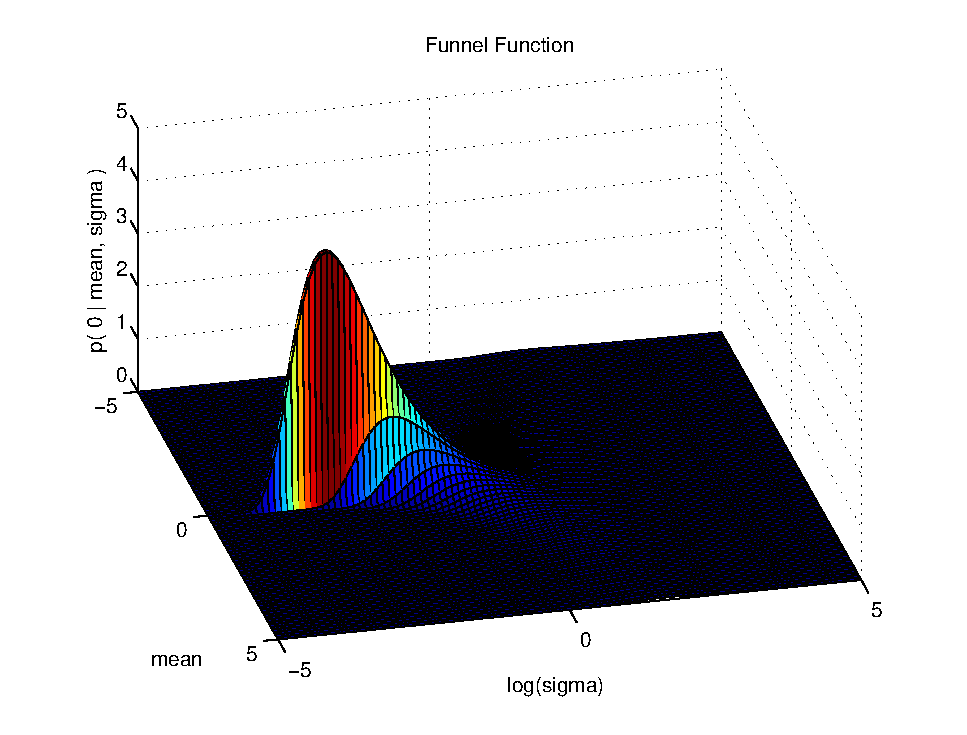
\includegraphics[width=0.45\textwidth]{figures/integrands/funnel.eps}
\caption{Radford Neal's funnel problem in 2 dimensions.}
\label{fig:funnel}
\end{figure}

%\begin{minipage}[t][0.45\paperheight][t]{0.45\paperwidth}
    % --- Automatically generated by latex_table.m ---
% Exported at 16-Feb-2012 13:24:18
\begin{table}[h!]
\caption{{\small
time taken (s)
}}
\label{tbl:time taken (s)}
\begin{center}
\begin{tabular}{l  r r r r r r r}
Integrand & \rotatebox{0}{ SMC }  & \rotatebox{0}{ AIS }  & \rotatebox{0}{ BMC AIS }  & \rotatebox{0}{ LBMC }  & \rotatebox{0}{ SBQ }  & \rotatebox{0}{ SBQ GPML }  & \rotatebox{0}{ BQ AIS }  \\ \midrule
simple & $\mathbf{0.023}$ & $1.306$ & $2.026$ & $1.251$ & $36.344$ & $12.158$ & $22.325$ \\
simple translated & $\mathbf{0.009}$ & $1.295$ & $1.948$ & $1.384$ & $ NaN$ & $ NaN$ & $23.192$ \\
simple scaled & $\mathbf{0.012}$ & $1.288$ & $1.897$ & $1.116$ & $37.762$ & $11.947$ & $21.611$ \\
easy 1d & $\mathbf{0.009}$ & $1.766$ & $2.064$ & $1.079$ & $45.821$ & $12.779$ & $ NaN$ \\
bumpy 1d & $\mathbf{0.007}$ & $1.126$ & $2.119$ & $1.144$ & $16.984$ & $26.335$ & $35.352$ \\
two spikes 1d & $\mathbf{0.016}$ & $2.781$ & $2.342$ & $1.888$ & $45.635$ & $ NaN$ & $45.693$ \\
two hills 1d & $\mathbf{0.020}$ & $2.781$ & $2.151$ & $1.091$ & $38.483$ & $11.402$ & $30.592$ \\
funnel 2d & $\mathbf{0.033}$ & $2.566$ & $2.241$ & $0.618$ & $67.442$ & $6.688$ & $9.770$ \\
friedman 3d & $\mathbf{0.371}$ & $12.441$ & $3.578$ & $0.447$ & $171.890$ & $7.807$ & $11.814$ \\
easy 4d & $\mathbf{0.010}$ & $1.924$ & $2.518$ & $0.666$ & $147.084$ & $10.071$ & $11.208$ \\
two spikes 4d & $\mathbf{0.012}$ & $2.997$ & $2.829$ & $ NaN$ & $ NaN$ & $ NaN$ & $ NaN$ \\
two hills 4d & $\mathbf{0.012}$ & $2.984$ & $2.321$ & $0.637$ & $219.580$ & $16.164$ & $11.057$ \\
friedman 7d & $\mathbf{0.356}$ & $11.618$ & $3.990$ & $4.756$ & $443.423$ & $57.409$ & $ NaN$ \\
\end{tabular}
\end{center}
\end{table}
% End automatically generated LaTeX

%\end{minipage}

% --- Automatically generated by latex_table.m ---
% Exported at 11-Feb-2012 20:59:11
\begin{table}[h!]
\caption{{\small
neg log density of truth at 100 samples
}}
\label{tbl:neg log density of truth at 100 samples}
\begin{center}
\begin{tabular}{l  r r r r r r}
Integrand & \rotatebox{0}{ SMC }  & \rotatebox{0}{ AIS }  & \rotatebox{0}{ BMC }  & \rotatebox{0}{ SBQ }  & \rotatebox{0}{ SBQ GPML }  & \rotatebox{0}{ BQ GPML AIS }  \\ \midrule
simple test & $-1.186$ & $233.335$ & $\mathbf{-2.942}$ & $-2.237$ & $-0.999$ & $-1.915$ \\
simple test transformed & $-1.186$ & $233.335$ & $\mathbf{-2.942}$ & $ NaN$ & $-1.104$ & $-1.915$ \\
easy 1d & $0.627$ & $\mathbf{-2.198}$ & $-1.189$ & $-0.453$ & $-1.145$ & $-1.353$ \\
bumpy 1d & $\mathbf{-3.050}$ & $>$ 1000 & $3.163$ & $-2.043$ & $ NaN$ & $0.867$ \\
bumpy 1d exp & $\mathbf{-3.518}$ & $>$ 1000 & $0.731$ & $-2.424$ & $ NaN$ & $0.015$ \\
two spikes 1d & $2.970$ & $24.156$ & $1.386$ & $ NaN$ & $\mathbf{0.120}$ & $1.220$ \\
two hills 1d & $2.970$ & $24.156$ & $1.386$ & $ NaN$ & $\mathbf{0.120}$ & $1.220$ \\
funnel 2d & $12.439$ & $52.654$ & $\mathbf{0.493}$ & $ NaN$ & $ NaN$ & $0.782$ \\
friedman 3d & $\mathbf{ NaN}$ & $ NaN$ & $ NaN$ & $ NaN$ & $ NaN$ & $ NaN$ \\
easy 4d & $0.601$ & $44.220$ & $0.410$ & $ NaN$ & $ NaN$ & $\mathbf{0.328}$ \\
two spikes 4d & $\mathbf{5.977}$ & $153.904$ & $23.489$ & $ NaN$ & $ NaN$ & $13.897$ \\
two hills 4d & $2.741$ & $687.308$ & $21.552$ & $ NaN$ & $ NaN$ & $\mathbf{0.356}$ \\
friedman 7d & $\mathbf{ NaN}$ & $ NaN$ & $ NaN$ & $ NaN$ & $ NaN$ & $ NaN$ \\
\end{tabular}
\end{center}
\end{table}
% End automatically generated LaTeX

% --- Automatically generated by latex_table.m ---
% Exported at 24-Feb-2012 15:01:01
\begin{table}[h!]
\caption{{\small
log squared error at 150 samples
}}
\label{tbl:log squared error at 150 samples}
\begin{center}
\begin{tabular}{l  r r r r r r r}
Integrand & \rotatebox{0}{ SMC }  & \rotatebox{0}{ AIS }  & \rotatebox{0}{ BMC }  & \rotatebox{0}{ BQ }  & \rotatebox{0}{ BQ* }  & \rotatebox{0}{ BBQ }  & \rotatebox{0}{ BBQ* }  \\ \midrule
simple & $-5.713$ & $-0.758$ & $-10.933$ & $-10.336$ & $-10.336$ & $-13.335$ & $\mathbf{-14.468}$ \\
bumpy 1d & $-4.859$ & $-6.866$ & $-3.286$ & $-3.466$ & $-3.466$ & $-2.594$ & $\mathbf{-10.106}$ \\
two spikes 1d & $-1.294$ & $\mathbf{-5.449}$ & $-0.821$ & $-0.574$ & $-0.574$ & $-1.724$ & $-3.628$ \\
two hills 1d & $-9.423$ & $-2.346$ & $-5.229$ & $-14.669$ & $-14.669$ & $\mathbf{-18.318}$ & $-18.317$ \\
funnel 2d & $-3.921$ & $-0.070$ & $-1.467$ & $-1.437$ & $-1.437$ & $-2.206$ & $\mathbf{-4.454}$ \\
easy 4d & $-6.665$ & $-4.655$ & $-4.073$ & $\mathbf{-6.785}$ & $-6.785$ & $-1.909$ & $-5.237$ \\
two spikes 4d & $-2.030$ & $3.664$ & $-3.540$ & $-2.275$ & $-2.275$ & $-2.322$ & $\mathbf{-4.772}$ \\
two hills 4d & $-0.707$ & $2.858$ & $-1.909$ & $-1.265$ & $-1.265$ & $-2.725$ & $\mathbf{-3.543}$ \\
real prawn 6d mean field & $\mathbf{-7.259}$ & $2.173$ & $-1.416$ & $-1.187$ & $-1.187$ & $2.084$ & $2.083$ \\
real prawn 6d markov & $\mathbf{-5.056}$ & $3.795$ & $3.000$ & $3.028$ & $3.028$ & $3.408$ & $3.412$ \\
real prawn 6d non-markov & $\mathbf{3.621}$ & $4.499$ & $3.710$ & $3.642$ & $3.642$ & $4.343$ & $4.346$ \\
\end{tabular}
\end{center}
\end{table}
% End automatically generated LaTeX


\begin{figure}
	\centering
	\setlength\fheight{4cm} 
	\setlength\fwidth{4cm}
	% This file was created by matlab2tikz v0.1.4.
% Copyright (c) 2008--2012, Nico Schlömer <nico.schloemer@gmail.com>
% All rights reserved.
% 
% 
% 
\begin{tikzpicture}

% defining custom colors
\definecolor{mycolor1}{rgb}{1,0.316227766016838,0.316227766016838}
\definecolor{mycolor2}{rgb}{0.316227766016838,1,0.316227766016838}
\definecolor{mycolor3}{rgb}{0.316227766016838,0.316227766016838,1}
\definecolor{mycolor4}{rgb}{0.632455532033676,0.632455532033676,0.316227766016838}
\definecolor{mycolor5}{rgb}{0.316227766016838,1,1}
\definecolor{mycolor6}{rgb}{0.948683298050514,0.316227766016838,0.948683298050514}


\begin{axis}[%
xmin=0, xmax=2,
ymin=0, ymax=2,
scale only axis,
width=\fwidth,
height=\fheight,
axis on top,
legend entries={SMC,AIS,BMC,SBQ,SBQ GPML,BQ GPML AIS,True value},
legend style={nodes=right}]
\end{axis}
\end{tikzpicture}

\end{figure}

\begin{figure}
	\centering
	\setlength\fheight{4cm} 
	\setlength\fwidth{4cm}
	% This file was created by matlab2tikz v0.1.4.
% Copyright (c) 2008--2011, Nico Schlömer <nico.schloemer@gmail.com>
% All rights reserved.
% 
\begin{tikzpicture}

% defining custom colors
\definecolor{mycolor1}{rgb}{1,0.1,0.1}
\definecolor{mycolor2}{rgb}{0.1,1,0.1}
\definecolor{mycolor3}{rgb}{0.1,0.1,1}
\definecolor{mycolor4}{rgb}{0.4,0.4,0.1}


\begin{semilogyaxis}[%
scale only axis,
width=\fwidth,
height=\fheight,
xmin=0, xmax=250,
ymin=1e-12, ymax=100,
yminorticks=true,
xlabel={Number of samples},
ylabel={Squared Distance to True Value},
title={$\text{sanity easy }1d$},
axis on top]
\addplot [
color=mycolor1,
solid,
line width=1.0pt
]
coordinates{
 (10,0.0104118)(20,0.0878559)(30,0.000230373)(40,0.0404657)(50,2.49412e-05)(100,0.0266959)(150,0.0138616)(200,0.0107615)(250,0.00431612) 
};

\addplot [
color=mycolor2,
solid,
line width=1.0pt
]
coordinates{
 (10,3.10822)(20,1.34249)(30,0.844347)(40,0.213341)(50,0.716871)(100,0.140222)(150,0.016806)(200,0.536118)(250,0.619462) 
};

\addplot [
color=mycolor3,
solid,
line width=1.0pt
]
coordinates{
 (10,0.0072074)(20,0.000121129)(30,0.00047062)(40,0.000418093)(50,2.8979e-06)(100,0.000176626)(150,0.000191801)(200,0.000140968)(250,1.89328e-06) 
};

\addplot [
color=mycolor4,
solid,
line width=1.0pt
]
coordinates{
 (10,0.0562805)(20,0.00845896)(30,0.000304203)(40,4.12692e-06)(50,5.77763e-08)(100,9.30455e-08)(150,2.19093e-12)(200,2.4049e-10)(250,1.95053e-06) 
};

\end{semilogyaxis}
\end{tikzpicture}

\end{figure}

\begin{figure}
	\centering
	\setlength\fheight{4cm} 
	\setlength\fwidth{4cm}
	% This file was created by matlab2tikz v0.1.4.
% Copyright (c) 2008--2011, Nico Schlömer <nico.schloemer@gmail.com>
% All rights reserved.
% 
\begin{tikzpicture}

% defining custom colors
\definecolor{mycolor1}{rgb}{1,0.1,0.1}
\definecolor{mycolor2}{rgb}{0.1,1,0.1}
\definecolor{mycolor3}{rgb}{0.1,0.1,1}
\definecolor{mycolor4}{rgb}{0.4,0.4,0.1}


\begin{semilogyaxis}[%
scale only axis,
width=\fwidth,
height=\fheight,
xmin=0, xmax=250,
ymin=1e-07, ymax=1,
yminorticks=true,
xlabel={Number of samples},
ylabel={Squared Distance to True Value},
title={$\text{sanity hard }1d$},
axis on top]
\addplot [
color=mycolor1,
solid,
line width=1.0pt
]
coordinates{
 (10,5.74619e-05)(20,0.000247289)(30,3.59312e-05)(40,6.72275e-05)(50,1.23698e-06)(100,0.000127854)(150,3.21991e-05)(200,1.04579e-05)(250,4.72674e-07) 
};

\addplot [
color=mycolor2,
solid,
line width=1.0pt
]
coordinates{
 (10,4.79482e-05)(20,0.000256417)(30,2.53732e-07)(40,6.493e-05)(50,5.35818e-05)(100,2.02467e-05)(150,4.07626e-05)(200,3.20687e-06)(250,3.67676e-05) 
};

\addplot [
color=mycolor3,
solid,
line width=1.0pt
]
coordinates{
 (10,0.394168)(20,0.0659873)(30,0.0712942)(40,0.0541693)(50,0.128508)(100,0.000364344)(150,0.000451895)(200,0.00975937)(250,0.000520116) 
};

\addplot [
color=mycolor4,
solid,
line width=1.0pt
]
coordinates{
 (10,0.00809716)(20,0.0112574)(30,0.0105948)(40,0.00719612)(50,0.00798252)(100,0.00888599)(150,0.00521284)(200,0.00898904)(250,0.00888976) 
};

\end{semilogyaxis}
\end{tikzpicture}
 
\end{figure}

\begin{figure}
	\centering
	\setlength\fheight{4cm} 
	\setlength\fwidth{4cm}
	% This file was created by matlab2tikz v0.1.4.
% Copyright (c) 2008--2011, Nico Schlömer <nico.schloemer@gmail.com>
% All rights reserved.
% 
\begin{tikzpicture}

% defining custom colors
\definecolor{mycolor1}{rgb}{1,0.1,0.1}
\definecolor{mycolor2}{rgb}{1,0.316228,0.316228}
\definecolor{mycolor3}{rgb}{0.1,1,0.1}
\definecolor{mycolor4}{rgb}{0.316228,1,0.316228}
\definecolor{mycolor5}{rgb}{0.1,0.1,1}
\definecolor{mycolor6}{rgb}{0.316228,0.316228,1}
\definecolor{mycolor7}{rgb}{0.4,0.4,0.1}
\definecolor{mycolor8}{rgb}{0.632456,0.632456,0.316228}


\begin{axis}[%
scale only axis,
width=\fwidth,
height=\fheight,
xmin=0, xmax=250,
ymin=-3.5, ymax=1.5,
xlabel={Number of samples},
ylabel={log evidence},
title={$\text{sanity easy }1d$},
axis on top,
legend entries={SMC,AIS,BMC,SBQ,True value},
legend style={nodes=right}]
\addplot [fill=mycolor1,opacity=1.000000e-01,draw=none] coordinates{ (10,1.0244)(20,1.36828)(30,0.657109)(40,0.215982)(50,0.237312)(100,0.543573)(150,0.305464)(200,0.207231)(250,0.0462748)(250,-2.06841)(200,-2.15329)(150,-2.22352)(100,-2.37033)(50,-2.38086)(40,-2.77184)(30,-2.78028)(20,-2.929)(10,-2.97385)};
\addplot [
color=mycolor2,
solid,
line width=1.0pt
]
coordinates{
 (10,-0.974728)(20,-0.780361)(30,-1.06159)(40,-1.27793)(50,-1.07177)(100,-0.913377)(150,-0.959031)(200,-0.973028)(250,-1.01107) 
};

\addplot [fill=mycolor3,opacity=1.000000e-01,draw=none] coordinates{ (10,-2.46961)(20,-2.14007)(30,-1.94472)(40,-1.50437)(50,-1.88688)(100,-1.4404)(150,-0.941737)(200,-1.79939)(250,-1.85773)(250,-1.86992)(200,-1.81854)(150,-0.952519)(100,-1.46205)(50,-1.96002)(40,-1.57293)(30,-2.04657)(20,-2.33078)(10,-3.20995)};
\addplot [
color=mycolor4,
solid,
line width=1.0pt
]
coordinates{
 (10,-2.83978)(20,-2.23542)(30,-1.99565)(40,-1.53865)(50,-1.92345)(100,-1.45123)(150,-0.947128)(200,-1.80897)(250,-1.86383) 
};

\addplot [fill=mycolor5,opacity=1.000000e-01,draw=none] coordinates{ (10,-1.13096)(20,-1.07824)(30,-1.08875)(40,-1.08759)(50,-1.07114)(100,-1.08407)(150,-1.0845)(200,-1.08418)(250,-1.07325)(250,-1.07325)(200,-1.08418)(150,-1.0845)(100,-1.08407)(50,-1.07114)(40,-1.08759)(30,-1.08875)(20,-1.07824)(10,-1.13096)};
\addplot [
color=mycolor6,
solid,
line width=1.0pt
]
coordinates{
 (10,-1.13096)(20,-1.07824)(30,-1.08875)(40,-1.08759)(50,-1.07114)(100,-1.08407)(150,-1.0845)(200,-1.08418)(250,-1.07325) 
};

\addplot [fill=mycolor7,opacity=1.000000e-01,draw=none] coordinates{ (10,-1.31243)(20,-1.16884)(30,-1.06143)(40,-1.08024)(50,-1.07788)(100,-1.07686)(150,-1.07677)(200,-1.07681)(250,-1.07657)(250,-1.07657)(200,-1.07681)(150,-1.07677)(100,-1.07686)(50,-1.07788)(40,-1.08024)(30,-1.06143)(20,-1.16884)(10,-1.31243)};
\addplot [
color=mycolor8,
solid,
line width=1.0pt
]
coordinates{
 (10,-1.31243)(20,-1.16884)(30,-1.06143)(40,-1.08024)(50,-1.07788)(100,-1.07686)(150,-1.07677)(200,-1.07681)(250,-1.07657) 
};

\addplot [
color=black,
solid,
line width=1.0pt
]
coordinates{
 (10,-1.07677)(20,-1.07677)(30,-1.07677)(40,-1.07677)(50,-1.07677)(100,-1.07677)(150,-1.07677)(200,-1.07677)(250,-1.07677) 
};

\end{axis}
\end{tikzpicture}
 
\end{figure}

\begin{figure}
	\centering
	\setlength\fheight{4cm} 
	\setlength\fwidth{4cm}
	% This file was created by matlab2tikz v0.1.4.
% Copyright (c) 2008--2011, Nico Schlömer <nico.schloemer@gmail.com>
% All rights reserved.
% 
\begin{tikzpicture}

% defining custom colors
\definecolor{mycolor1}{rgb}{1,0.1,0.1}
\definecolor{mycolor2}{rgb}{1,0.316228,0.316228}
\definecolor{mycolor3}{rgb}{0.1,1,0.1}
\definecolor{mycolor4}{rgb}{0.316228,1,0.316228}
\definecolor{mycolor5}{rgb}{0.1,0.1,1}
\definecolor{mycolor6}{rgb}{0.316228,0.316228,1}


\begin{axis}[%
scale only axis,
width=\fwidth,
height=\fheight,
xmin=0, xmax=250,
ymin=-1.2, ymax=0.2,
xlabel={Number of samples},
ylabel={log evidence},
title={$\text{sanity hard }1\text{d exp}$},
axis on top]
\addplot [fill=mycolor1,opacity=1.000000e-01,draw=none] coordinates{ (10,0.0679381)(20,0.0489932)(30,0.0272247)(40,0.0145464)(50,0.019785)(100,0.00990157)(150,0.00933141)(200,0.00933643)(250,0.0119235)(250,-0.006067)(200,-0.0103702)(150,-0.0135499)(100,-0.0192566)(50,-0.0203241)(40,-0.028431)(30,-0.0261668)(20,-0.0148092)(10,-0.0315284)};
\addplot [
color=mycolor2,
solid,
line width=1.0pt
]
coordinates{
 (10,0.0182049)(20,0.017092)(30,0.000528989)(40,-0.00694232)(50,-0.000269519)(100,-0.00467751)(150,-0.00210926)(200,-0.000516905)(250,0.00292827) 
};

\addplot [fill=mycolor3,opacity=1.000000e-01,draw=none] coordinates{ (10,0.0190779)(20,0.0125642)(30,0.0052372)(40,0.00724723)(50,0.00535601)(100,-0.00420427)(150,0.00107048)(200,0.0103163)(250,-0.00209716)(250,-0.00219345)(200,0.0101808)(150,0.000877285)(100,-0.00456792)(50,0.00448589)(40,0.00604854)(30,0.00326893)(20,0.0092607)(10,0.00219186)};
\addplot [
color=mycolor4,
solid,
line width=1.0pt
]
coordinates{
 (10,0.0106349)(20,0.0109124)(30,0.00425307)(40,0.00664788)(50,0.00492095)(100,-0.00438609)(150,0.000973882)(200,0.0102485)(250,-0.0021453) 
};

\addplot [fill=mycolor5,opacity=1.000000e-01,draw=none] coordinates{ (10,-0.0601931)(20,0.0342545)(30,0.0284588)(40,0.0405251)(50,0.0454247)(100,-4.31345e-05)(150,-0.000621986)(200,-0.00024921)(250,0.00128438)(250,-0.0257425)(200,-0.0263382)(150,-0.0460361)(100,-0.254534)(50,-0.453844)(40,-0.45751)(30,-0.462778)(20,-0.246622)(10,-1.09873)};
\addplot [
color=mycolor6,
solid,
line width=1.0pt
]
coordinates{
 (10,-0.579464)(20,-0.106184)(30,-0.21716)(40,-0.208492)(50,-0.20421)(100,-0.127289)(150,-0.023329)(200,-0.0132937)(250,-0.012229) 
};

\addplot [
color=black,
solid,
line width=1.0pt
]
coordinates{
 (10,0.00249844)(20,0.00249844)(30,0.00249844)(40,0.00249844)(50,0.00249844)(100,0.00249844)(150,0.00249844)(200,0.00249844)(250,0.00249844) 
};

\end{axis}
\end{tikzpicture}

\end{figure}

\section{Discussion}

\section{Conclusions}

\section*{Acknowledgements}

\bibliography{bub}
\bibliographystyle{icml2012}

\end{document} 


